% Arquivo LaTeX de exemplo de dissertação/tese a ser apresentada à CPG do IME-USP
%
% Criação: Jesús P. Mena-Chalco
% Revisão: Fabio Kon e Paulo Feofiloff
% Adaptação para UTF8, biblatex e outras melhorias: Nelson Lago
%
% Except where otherwise indicated, these files are distributed under
% the MIT Licence. The example text, which includes the tutorial and
% examples as well as the explanatory comments in the source, are
% available under the Creative Commons Attribution International
% Licence, v4.0 (CC-BY 4.0) - https://creativecommons.org/licenses/by/4.0/


%%%%%%%%%%%%%%%%%%%%%%%%%%%%%%%%%%%%%%%%%%%%%%%%%%%%%%%%%%%%%%%%%%%%%%%%%%%%%%%%
%%%%%%%%%%%%%%%%%%%%%%%%%%%%%%% PREÂMBULO LaTeX %%%%%%%%%%%%%%%%%%%%%%%%%%%%%%%%
%%%%%%%%%%%%%%%%%%%%%%%%%%%%%%%%%%%%%%%%%%%%%%%%%%%%%%%%%%%%%%%%%%%%%%%%%%%%%%%%

% A opção twoside (frente-e-verso) significa que a aparência das páginas pares
% e ímpares pode ser diferente. Por exemplo, as margens podem ser diferentes ou
% os números de página podem aparecer à direita ou à esquerda alternadamente.
% Mas nada impede que você crie um documento "só frente" e, ao imprimir, faça
% a impressão frente-e-verso.
%
% Aqui também definimos a língua padrão do documento
% (a última da lista) e línguas adicionais.
%\documentclass[12pt,twoside,brazilian,english]{book}
\documentclass[12pt,twoside,english,brazilian]{book}

% Ao invés de definir o tamanho das margens, vamos definir os tamanhos do
% texto, do cabeçalho e do rodapé, e deixamos a package geometry calcular
% o tamanho das margens em função do tamanho do papel. Assim, obtemos o
% mesmo resultado impresso, mas com margens diferentes, se o tamanho do
% papel for diferente.
\usepackage[a4paper]{geometry}

\geometry{
  textwidth=152mm,
  hmarginratio=12:17, % 24:34 -> com papel A4, 24mm + 152mm + 34mm = 210mm
  textheight=237mm,
  vmarginratio=8:7, % 32:28 -> com papel A4, 32mm + 237mm + 28mm = 297mm
  headsep=11mm, % distância entre a base do cabeçalho e o texto
  headheight=21mm, % qualquer medida grande o suficiente, p.ex., top - headsep
  footskip=10mm,
  marginpar=20mm,
  marginparsep=5mm,
}

% Vários pacotes e opções de configuração genéricos; para personalizar o
% resultado, modifique estes arquivos.
%%%%%%%%%%%%%%%%%%%%%%%%%%%%%%%%%%%%%%%%%%%%%%%%%%%%%%%%%%%%%%%%%%%%%%%%%%%%%%%%
%%%%%%%%%%%%%%%%%%%%%%% CONFIGURAÇÕES E PACOTES BÁSICOS %%%%%%%%%%%%%%%%%%%%%%%%
%%%%%%%%%%%%%%%%%%%%%%%%%%%%%%%%%%%%%%%%%%%%%%%%%%%%%%%%%%%%%%%%%%%%%%%%%%%%%%%%

% Vários comandos auxiliares para o desenvolvimento de packages e classes;
% aqui, usamos em alguns comandos de formatação e condicionais.
\usepackage{etoolbox}
%\RequirePackage{pdftexcmds}
\usepackage{letltxmacro}
%\usepackage{ltxcmds}

% LaTeX 3
\usepackage{expl3}
\usepackage{xparse}

%\usepackage{filehook}

% Detecta se estamos usando pdftex, luatex, xetex etc.
\usepackage{iftex}

%\usepackage{xfp} % Floating-point calculations

\usepackage{regexpatch}

% O projeto LaTeX3 renomeou algumas macros em 2019-03-05 e removeu
% a compatibilidade com os nomes antigos em 2020-07-17 a partir de
% 2021-01-01 (veja o arquivo l3deprecation.dtx e o changelog em
% https://github.com/latex3/latex3/blob/main/l3kernel/CHANGELOG.md).
% Isso afetou a package regexpatch: versões antigas da package não
% funcionam com versões novas de LaTeX e vice-versa. Infelizmente,
% ubuntu 21.04 (hirsute) e debian 11 (bullseye) incluem essas versões
% incompatíveis e, portanto, a package regexpatch não funciona nesses
% ambientes. Talvez fosse possível contornar esse problema com a
% package latexrelease, mas isso afetaria muitos outros recursos.
% Ao invés disso, vamos restaurar manualmente a compatibilidade.
% TODO: remover isto após debian bullseye se tornar obsoleta,
%       provavelmente no final de 2024.
\makeatletter
\ExplSyntaxOn
\@ifpackagelater{regexpatch}{2021/03/21}
  {} % Se regexpatch é "nova", expl3 deve ser também; nada a fazer
  {
    % Talvez o correto seja 2021/01/01, mas na prática o resultado é o mesmo
    \@ifpackagelater{expl3}{2020/07/17}
      {
        % As versões são incompatíveis; vamos recuperar as macros preteridas
        \cs_gset:Npn \token_get_prefix_spec:N { \cs_prefix_spec:N }
        \cs_gset:Npn \token_get_arg_spec:N { \cs_argument_spec:N }
        \cs_gset:Npn \token_get_replacement_spec:N { \cs_replacement_spec:N }
      }
      {} % As duas packages são antigas e, portanto, compatíveis entre si
  }
\ExplSyntaxOff
\makeatother

% Algumas packages dependem de xpatch e tentam carregá-la, causando conflitos
% com regexpatch. Como regexpatch oferece todos os recursos de xpatch (ela
% é uma versão estendida de xpatch, mas ainda considerada experimental), vamos
% fazê-las acreditar que xpatch já foi carregada.
\makeatletter
\@ifpackagelater{regexpatch}{2020/10/06}
    {\expandafter\xdef\csname ver@xpatch.sty\endcsname{2020/03/25}}
    {\expandafter\xdef\csname ver@xpatch.sty\endcsname{2012/10/02}}
\makeatother

% Acrescenta a correção deste bug (contida na release 2018-11-28):
% https://github.com/latex3/latex2e/issues/94 . Se a correção não
% puder ser aplicada, temos uma versão de LaTeX que já a incorpora.
% Esse bug afeta apenas textos em duas colunas.
% TODO: remover após ubuntu 18.04 se tornar obsoleta (abril/2023)
\makeatletter
\patchcmd\@combinedblfloats{\box\@outputbox}{\unvbox\@outputbox}{}{}
\makeatother

% Arithmetic expressions in \set{length,counter} & \addto{length,counter};
% commands \widthof, \heightof, \depthof, \totalheightof, \settototalheight
\usepackage{calc}

% Algumas packages "padrão" da AMS, que são praticamente obrigatórias.
% Algumas delas devem ser carregadas antes de unicode-math ou das
% definições das fontes do documento. É preciso carregar amsthm após
% amsmath para o comando \qedhere funcionar dentro do ambiente align.
\usepackage{amssymb}
\usepackage{amsmath}
\usepackage{amsthm}

% "fontenc" é um parâmetro do NFSS (sistema de gestão de fontes do
% LaTeX; consulte "texdoc fntguide" e "texdoc fontenc"). O default
% é OT1, mas ele tem algumas limitações; a mais importante é que,
% com ele, palavras acentuadas não podem ser hifenizadas. Por
% conta disso, quase todos os documentos LaTeX utilizam o fontenc
% T1. A escolha do fontenc tem consequências para as fontes que
% podem ser usadas com NFSS; hoje em dia T1 tem mais opções de
% qualidade, então não se perde nada em usá-lo. A package fontspec
% (para gestão de fontes usando outro mecanismo, compatível apenas
% com lualatex e xelatex) carrega fontenc automaticamente, mas
% usando outra codificação ("TU" e não "T1"). Ainda assim, é útil
% carregar o fontenc T1 (antes de carregar fontspec!) para o caso
% de alguma fonte "antiga" ser utilizada no documento (embora isso
% não seja recomendado: lualatex e xelatex só são capazes de
% hifenizar palavras acentuadas com o fontenc TU).
\usepackage[T1]{fontenc}

\ifPDFTeX
  % O texto está escrito em utf8.
  \usepackage[utf8]{inputenc}

  % Várias packages que definem as fontes do documento carregam fontaxes,
  % mas carregamos aqui porque, com qualquer fonte, ela permite utilizar
  % small caps + itálico. Algumas raras packages de fontes podem causar
  % conflitos com fontaxes, em geral por utilizarem a package "concorrente"
  % nfssext-cfr.
  %
  % TODO A funcionalidade pela qual faz sentido carregar fontaxes aqui
  %      (small caps + itálico) foi incorporada ao kernel do LaTeX na
  %      versão 2020-02-02, então está em TeXLive 2021. Remover isto
  %      quando arxiv usar TeXLive >= 2021 e ubuntu 20.04 (focal) for
  %      descontinuada (abril de 2025). As packages que precisam de
  %      fontaxes podem continuar a carregá-la sem problemas.
  \usepackage{fontaxes}

  % LaTeX substitui algumas sequências de caracteres, como
  % "fi", "fl" e outras, por caracteres especiais ("ligaduras").
  % Para que seja possível fazer copiar/colar ou buscas por
  % textos contendo essas ligaduras, o arquivo PDF precisa
  % conter uma tabela indicando quais são elas. Com fontes
  % OTF (LuaLaTeX ou XeLaTeX) isso não costuma ser um problema,
  % mas com pdfLaTeX pode ser. Estes dois comandos (que só
  % existem no pdfLaTeX) incluem uma tabela genérica que
  % funciona para a maioria das fontes. Veja a seção 5 de
  % http://www.tug.org/TUGboat/Articles/tb29-1/tb91thanh-fonts.pdf
  % Note que alguns visualizadores de PDF tentam "adivinhar"
  % o conteúdo da tabela quando ela está incompleta ou não
  % existe, então copiar/colar e buscas podem funcionar em
  % alguns visualizadores e em outros não.
  %
  % TODO Isto foi incluído no kernel do LaTeX versão 2021-06-01,
  %      então está em TeXLive 2022. Remover isto quando arxiv
  %      usar TeXLive >= 2022 e ubuntu 22.04 (jammy) for
  %      descontinuada (abril de 2027).
  \input glyphtounicode.tex
  \pdfgentounicode=1
\else
  % Não é preciso carregar inputenc com LuaTeX e XeTeX, pois
  % com eles utf8 é obrigatório.
  \usepackage{fontspec}

  % Ao invés de usar o sistema tradicional de LaTeX para gerir
  % as fontes matemáticas, utiliza as extensões matemáticas do
  % formato otf definidas pela microsoft. Ao ativar esta package
  % o mecanismo tradicional não funciona mais! Há poucas fontes
  % com suporte a unicode-math.
  \usepackage{unicode-math}
\fi

% Acesso a símbolos adicionais, como \textrightarrow, \texteuro etc.,
% disponíveis na maioria das fontes através do fontenc TS1 ou mudando
% momentaneamente para computer modern/latin modern. Raramente útil
% com lualatex/xelatex, mas não causa problemas. Várias packages de
% fontes carregam textcomp, às vezes com opções específicas; assim,
% para evitar problemas, vamos carregá-la no final do preâmbulo para
% o caso de ela não ter sido carregada antes.
%
% TODO A funcionalidade oferecida por textcomp foi incorporada ao kernel
%      do LaTeX na versão 2020-02-02, então está em TeXLive 2021. Remover
%      isto quando arxiv usar TeXLive >= 2021 e ubuntu 20.04 (focal) for
%      descontinuada (abril de 2025). As packages que precisam de textcomp
%      podem continuar a carregá-la sem problemas.
\AtBeginDocument{\usepackage{textcomp}}

% TeXLive 2018 inclui a versão 2.7a da package microtype e a versão
% 1.07 de luatex. Essa combinação faz aparecer um bug:
% https://tex.stackexchange.com/a/476742
% Aqui, aplicamos a solução sugerida, que não tem "contra-indicações".
% TODO: remover após ubuntu 18.04 se tornar obsoleta (abril/2023)
\ifLuaTeX
  \usepackage{luatexbase}
\fi

% microajustes no tamanho das letras, espaçamento etc. para melhorar
% a qualidade visual do resultado.
\usepackage{microtype}

% Alguns "truques" (sujos?) para minimizar over/underfull boxes.
%
% Para fazer um texto justificado, é preciso modificar o tamanho dos espaços
% em cada linha para mais ou para menos em relação ao seu tamanho ideal. Para
% escolher as quebras de linha, TeX vai percorrendo o texto procurando lugares
% possíveis para quebrar as linhas considerando essa flexibilidade mas dentro
% de um certo limite mínimo/máximo. Nesse processo, ele associa a cada possível
% linha o valor *badness*, que é o nível de distorção do tamanho dos espaços
% daquela linha em relação ao ideal, e ignora opções que tenham badness muito
% grande (esse limite é dado por \tolerance). Depois de encontradas todas
% as possíveis quebras de linha e a badness de cada uma, TeX calcula as
% *penalties* das quebras encontradas, que são uma medida de quebras "ruins".
% Por exemplo, na configuração padrão, quebrar uma linha hifenizando uma
% palavra gera uma penalty de 50; já uma quebra que faça a última linha
% do parágrafo ficar sozinha na página seguinte gera uma penalty de 150.
% Finalmente, TeX calcula a "feiúra" de cada possível linha (demerits)
% com base na badness e nas penalties e escolhe a solução que minimiza os
% demerits totais do parágrafo. Os comandos \linebreak e \pagebreak funcionam
% simplesmente acrescentando uma penalty negativa ao lugar desejado para a
% quebra.
%
% Para cada fonte, o espaço entre palavras tem um tamanho ideal, um
% tamanho mínimo e um tamanho máximo (é possível obter os valores com
% \number\fontdimenX\font\relax, veja https://tex.stackexchange.com/q/88991 ).
% TeX nunca reduz um espaço para menos que o mínimo da fonte, mas pode
% aumentá-lo para mais que o máximo. Se os espaços de uma linha ficam
% com o tamanho ideal, a badness da linha é 0; se o tamanho é
% reduzido/aumentado 50% do mínimo/máximo, a badness da linha é 12; se
% o tamanho é reduzido/aumentado para o mínimo/máximo, a badness é 100,
% e assim por diante. O valor máximo possível para badness é 10.000, que
% significa "badness infinita". Como é feito o cálculo: se as medidas
% do espaço definidas pela fonte são "x plus y minus z" e o tamanho
% final do espaço é "x + k*y" ou "x - k*z", a badness é 100*(k^3). Com
% Libertinus corpo 12, os valores são "3pt plus 1.5pt minus .9996pt",
% Então se o espaço tiver sido aumentado para 3.75pt, o fator é 0.5 e
% a badness é 100*(.5^3) = 12.
%
% \tolerance indica a badness máxima que TeX aceita para uma linha; seu valor
% default é 200. Assim, aumentar para, digamos, 300 ou 400, permite que
% TeX escolha parágrafos com maior variação no espaçamento entre as palavras.
% No entanto, no cálculo de demerits, a badness e as penalties de cada linha
% são elevadas ao quadrado, então TeX geralmente prefere escolher outras
% opções no lugar de uma linha com espaçamento ruim. Por exemplo, órfãs/viúvas
% têm demerit de 22.500 e dois hífens seguidos têm demerit de 10.000; já uma
% linha com badness 400 tem demerit 160.000. Portanto, não é surpreendente que
% a maioria dos parágrafos tenha demerits abaixo de 40.000, quase todos abaixo
% de 100.000 e praticamente nenhum acima de 1.000.000. Isso significa que, para
% a grande maioria dos parágrafos, aumentar \tolerance não faz diferença: uma
% linha com badness 400 nunca será efetivamente escolhida se houver qualquer
% outra opção com badness menor. Também fica claro que não há muita diferença
% real entre definir \tolerance como 800 ou 9.999 (a não ser fazer TeX
% trabalhar mais desnecessariamente).
%
% O problema muda de figura se TeX não consegue encontrar uma solução. Isso
% pode acontecer em dois casos: (1) o parágrafo tem ao menos uma linha que não
% pode ser quebrada com badness < 10.000 ou (2) o parágrafo tem ao menos uma
% linha que não pode ser quebrada com badness < tolerance (mas essa badness é
% menor que 10.000).
%
% No primeiro caso, se houver várias possibilidades de linhas que não podem ser
% quebradas, TeX não vai ser capaz de compará-las e escolher a melhor: todas
% têm a badness máxima (10.000) e, portanto, a que gerar menos deméritos no
% restante do parágrafo será a escolhida. Na realidade, no entanto, essas
% linhas *não* são igualmente ruins entre si, o que pode levar TeX a fazer uma
% má escolha. Para evitar isso, TeX tenta novamente aplicando
% \emergencystretch, que "faz de conta" que o tamanho máximo ideal dos espaços
% da linha é maior que o definido na fonte. Isso reduz a badness de todas as
% linhas, o que soa parecido com aumentar \tolerance. Há três diferenças, no
% entanto: (1) essa mudança só afeta os parágrafos que falharam; (2) soluções
% que originalmente teriam badness = 10.000 (e, portanto, seriam vistas como
% equivalentes) podem ser avaliadas e comparadas entre si; e (3) como a badness
% de todas as linhas diminui, a possibilidade de outras linhas que
% originalmente tinham badness alta serem escolhidas aumenta. Esse último ponto
% significa que \emergencystretch pode fazer TeX escolher linhas mais
% espaçadas, fazendo o espaçamento do parágrafo inteiro aumentar e, portanto,
% tornando o resultado mais homogêneo mesmo com uma linha particularmente ruim.
%
% É esse último ponto que justifica o uso de \emergencystretch no segundo caso
% também: apenas aumentar a tolerância, nesse caso, poderia levar TeX a
% diagramar uma linha ruim em meio a um parágrafo bom, enquanto
% \emergencystretch pode fazer TeX aumentar o espaçamento de maneira geral no
% parágrafo, minimizando o contraste da linha problemática com as demais.
% Colocando a questão de outra maneira, aumentar \tolerance para lidar com
% esses parágrafos problemáticos pode fazê-los ter uma linha especialmente
% ruim, enquanto \emergencystretch pode dividir o erro entre várias linhas.
% Assim, definir \tolerance em torno de 800 parece razoável: no caso geral,
% não há diferença e, se um desses casos difíceis não pode ser resolvido com
% uma linha de badness até 800, \emergencystretch deve ser capaz de gerar um
% resultado igual ou melhor.
%
% Penalties & demerits: https://tex.stackexchange.com/a/51264
% Definições (fussy, sloppy etc.): https://tex.stackexchange.com/a/241355
% Mais definições (hfuzz, hbadness etc.): https://tex.stackexchange.com/a/50850
% Donald Arseneau defendendo o uso de \sloppy: https://groups.google.com/d/msg/comp.text.tex/Dhf0xxuQ66E/QTZ7aLYrdQUJ
% Artigo detalhado sobre \emergencystretch: https://www.tug.org/TUGboat/tb38-1/tb118wermuth.pdf
% Esse artigo me leva a crer que algo em torno de 1.5em é suficiente

\tolerance=800
\hyphenpenalty=100 % Default 50; se o texto é em 2 colunas, 50 é melhor
\setlength{\emergencystretch}{1.5em}

% Não gera warnings para Overfull menor que 1pt
\hfuzz=1pt
\vfuzz\hfuzz

% Não gera warnings para Underfull com badness < 1000
\hbadness=1000
\vbadness=1000

% Por padrão, o algoritmo LaTeX para textos não-justificados é (muito) ruim;
% este pacote implementa um algoritmo bem melhor
\usepackage[newcommands]{ragged2e}

% ragged2e funciona porque permite que LaTeX hifenize palavras em textos
% não-justificados quando necessário. No caso de textos centralizados,
% no entanto, isso em geral não é desejável. Assim, newcommands não é
% interessante para \centering e \begin{center}. newcommands também
% causa problemas com legendas se o float correspondente usa \centering
% (o que é muito comum). Assim, vamos voltar \centering e \begin{center}
% à definição padrão.
\let\centering\LaTeXcentering
\let\center\LaTeXcenter
\let\endcenter\endLaTeXcenter

% Com ragged2e e a opção "newcommands", textos curtos não-justificados
% podem gerar warnings sobre "underfull \hbox". Não há razão para pensar
% muito nesses warnings, então melhor desabilitá-los.
% https://tex.stackexchange.com/a/18019
\makeatletter
\gappto{\raggedright}{\hbadness=\@M}
\gappto{\RaggedRight}{\hbadness=\@M}
\gappto{\raggedleft}{\hbadness=\@M}
\gappto{\RaggedLeft}{\hbadness=\@M}
\gappto{\Centering}{\hbadness=\@M} % not \centering
\gappto{\flushleft}{\hbadness=\@M}
\gappto{\FlushLeft}{\hbadness=\@M}
\gappto{\flushright}{\hbadness=\@M}
\gappto{\FlushRight}{\hbadness=\@M}
\gappto{\Center}{\hbadness=\@M} % not \center
\makeatother

% Espaçamento entre linhas configurável (\singlespacing, \onehalfspacing etc.)
\usepackage{setspace}

% LaTeX às vezes coloca notas de rodapé logo após o final do texto da
% página ao invés de no final da página; este pacote evita isso e faz
% notas de rodapé funcionarem corretamente em títulos de seções.
% Esta package deve ser carregada depois de setspace.
\usepackage[stable,bottom]{footmisc}

% Se uma página está vazia, não imprime número de página ou cabeçalho
\usepackage{emptypage}

% hyperref deve preferencialmente ser carregada próximo ao final
% do preâmbulo mas, para o caso de alguma package forçar a sua
% carga antes de executarmos \usepackage explicitamente, vamos
% garantir que estas opções estejam ativas.
\PassOptionsToPackage{
  unicode=true,
  pdfencoding=unicode,
  plainpages=false,
  pdfpagelabels,
  bookmarksopen=true,
  breaklinks=true,
  %hyperfootnotes=false, % polui desnecessariamente com bordercolor
}{hyperref}

% Carrega nomes de cores disponíveis (podem ser usados com hyperref e listings)
\usepackage[hyperref,svgnames,x11names,table]{xcolor}

% LaTeX oferece 2 pares de comandos nativos para mudar textos para caixa
% alta ou baixa: \uppercase ou \lowercase (TeX "puro") e \MakeUppercase
% ou \MakeLowecase (LaTeX), mas esses comandos têm algumas limitações
% (https://tug.org/TUGboat/tb41-1/tb127wright-case.pdf ). Esta package
% define os comandos \MakeTextUppercase e \MakeTextLowercase que resolvem
% isso.
% TODO: quando TeXLive 2023 for a versão mais antiga de LaTeX a que
%       estivermos dando suporte, podemos eliminar a package textcase
%       e usar \MakeUppercase e \MakeLowercase diretamente. A partir
%       dessa versão, essas macros usam \text_[upper|lower]case:n de
%       expl3.
\usepackage{textcase}

% Em documentos frente-e-verso, LaTeX faz o final da página terminar sempre
% no mesmo lugar (exceto no final dos capítulos). Esse comportamento pode ser
% ativado explicitamente com o comando "\flushbottom". Mas se, por alguma
% razão, o volume de texto na página é "pequeno", essa página vai ter espaços
% verticais artificialmente grandes. Uma solução para esse problema é utilizar
% "\raggedbottom" (padrão em documentos que não são frente-e-verso): com essa
% opção, as páginas podem terminar em alturas ligeiramente diferentes. Outra
% opção é corrigir manualmente cada página problemática, por exemplo com o
% comando "\enlargethispage".
%\raggedbottom
\flushbottom

% Por padrão, LaTeX coloca uma espaço aumentado após sinais de pontuação;
% Isso não é tão bom quanto alguns TeX-eiros defendem :) .
% Esta opção desabilita isso e, consequentemente, evita problemas com
% "id est" (i.e.) e "exempli gratia" (e.g.)
\frenchspacing

% Mais recursos para trechos de texto "puro" (tabs, quebras de linha etc.
% não são modificados), além do ambiente "\begin{comment}".
\usepackage{verbatim}

% Durante o processamento, LaTeX procura por arquivos adicionais necessários
% (tanto componentes do próprio LaTeX, como packages e fontes, quanto partes
% do conteúdo em si, como imagens carregadas com \includegraphics ou arquivos
% solicitados com \input ou \include) no diretório de instalação e também
% no diretório atual (ou seja, o diretório do projeto). Assim, normalmente
% é preciso usar caminhos relativos para incluir arquivos de subdiretórios:
% "\input{diretorio/arquivo}". No entanto, há duas limitações:
%
% 1. É necessário dizer "\input{diretorio/arquivo}" mesmo quando o arquivo
%    que contém esse comando já está dentro do subdiretório.
%
% 2. Isso não deve ser usado para packages ("\usepackage{diretorio/package}"),
%    embora na prática funcione.
%
% Há três maneiras recomendadas de resolver esses problemas:
%
% 1. Acrescentando os diretórios desejados ao arquivo texmf.cnf
%
% 2. Acrescentando os diretórios desejados às variáveis de ambiente
%    TEXINPUTS e BSTINPUTS
%
% 3. Colocando os arquivos adicionais na árvore TEXMF (geralmente, no
%    diretório texmf dentro do diretório do usuário).
%
% Essas soluções, no entanto, não podem ser automatizadas por este modelo
% e são um tanto complicadas para usuários menos experientes. Veja mais a
% respeito na seção 5 de "texdoc kpathsea" e em
% https://www.overleaf.com/learn/latex/Articles/An_introduction_to_Kpathsea_and_how_TeX_engines_search_for_files .
%
% A package import pode solucionar o primeiro problema, mas exige o uso
% de outro comando no lugar de \input, então não a usamos aqui.
%\usepackage{import}
%
% Uma solução mais simples é acrescentar os diretórios desejados à macro
% \input@path, originalmente criada para resolver um problema relacionado
% à portabilidade. Seu uso não é normalmente recomendado por razões de
% desempenho, mas no nosso caso (em que adicionamos apenas um diretório
% com poucos arquivos e com máquinas modernas) isso não é um problema. Veja
% https://tex.stackexchange.com/questions/241828/define-path-for-packages-in-the-latex-file-analog-of-inputpath-or-graphicspa#comment705011_241832
\csappto{input@path}{{extras/}}

%%%%%%%%%%%%%%%%%%%%%%%%%%%%%%%%%%%%%%%%%%%%%%%%%%%%%%%%%%%%%%%%%%%%%%%%%%%%%%%%
%%%%%%%%%%%%%%%%%%%%%%%%%%%%%%%%%%% LÍNGUAS %%%%%%%%%%%%%%%%%%%%%%%%%%%%%%%%%%%%
%%%%%%%%%%%%%%%%%%%%%%%%%%%%%%%%%%%%%%%%%%%%%%%%%%%%%%%%%%%%%%%%%%%%%%%%%%%%%%%%

\makeatletter
\ExplSyntaxOn

% We need to have at least some variant of Portuguese and of English
% loaded to generate the abstract/resumo, palavras-chave/keywords etc.
% We will make sure that both languages are present in the class options
% list by adding them if needed. With this, these options become global
% and therefore are seen by all packages (among them, babel).
%
% babel traditionally uses "portuguese", "brazilian", "portuges", or
% "brazil" to support the Portuguese language, using .ldf files. babel
% is also in the process of implementing a new scheme, using .ini
% files, based on the concept of "locales" instead of "languages". This
% mechanism uses the names "portuguese-portugal", "portuguese-brazil",
% "portuguese-pt", "portuguese-br", "portuguese", "brazilian", "pt",
% "pt-PT", and "pt-BR" (i.e., neither "portuges" nor "brazil"). To avoid
% compatibility problems, let's stick with "brazilian" or "portuguese"
% by substituting portuges and brazil if necessary.

\NewDocumentCommand\@IMEportugueseAndEnglish{m}{

  % Make sure any instances of "portuges" and "brazil" are replaced
  % by "portuguese" e "brazilian"; other options are unchanged.
  \seq_gclear_new:N \l_tmpa_seq
  \seq_gclear_new:N \l_tmpb_seq
  \seq_gset_from_clist:Nc \l_tmpa_seq {#1}

  \seq_map_inline:Nn \l_tmpa_seq{
    \def\@tempa{##1}
    \ifstrequal{portuges}{##1}
      {
        \GenericInfo{sbc2019}{}{Substituting~language~portuges~->~portuguese}
        \def\@tempa{portuguese}
      }
      {}
    \ifstrequal{brazil}{##1}
      {
        \GenericInfo{}{Substituting~language~brazil~->~brazilian}
        \def\@tempa{brazilian}
      }
      {}
    \seq_gput_right:NV \l_tmpb_seq {\@tempa}
  }

  % Remove the leftmost duplicates (default is to remove the rightmost ones).
  % Necessary in case the user did "portuges,portuguese", "brazil,brazilian"
  % or some variation: When we substitute the language, we end up with the
  % exact same language twice, which may mess up the main language selection.
  \seq_greverse:N \l_tmpb_seq
  \seq_gremove_duplicates:N \l_tmpb_seq
  \seq_greverse:N \l_tmpb_seq

  % If the user failed to select some variation of English and Portuguese,
  % we add them here. We also remember which ones of portuguese/brazilian,
  % english/american/british etc. were selected.
  \exp_args:Nnx \regex_extract_all:nnNTF
    {\b(portuguese|brazilian)\b}
    {\seq_use:Nn \l_tmpb_seq {,}}
    \l_tmpa_tl
    {
      \tl_reverse:N \l_tmpa_tl
      \xdef\@IMEpt{\tl_head:N \l_tmpa_tl}
    }
    {
      \seq_gput_left:Nn \l_tmpb_seq {brazilian}
      \gdef\@IMEpt{brazilian}
    }

  \exp_args:Nnx \regex_extract_all:nnNTF
    {\b(english|american|USenglish|canadian|british|UKenglish|australian|newzealand)\b}
    {\seq_use:Nn \l_tmpb_seq {,}}
    \l_tmpa_tl
    {
      \tl_reverse:N \l_tmpa_tl
      \xdef\@IMEen{\tl_head:N \l_tmpa_tl}
    }
    {
      \seq_gput_left:Nn \l_tmpb_seq {english}
      \gdef\@IMEen{english}
    }

  \exp_args:Nc \xdef {#1} {\seq_use:Nn \l_tmpb_seq {,}}
}


% https://tex.stackexchange.com/a/43541
% This message is part of a larger thread that discusses some
% limitations of this method, but it is enough for us here.
\def\@getcl@ss#1.cls#2\relax{\def\@currentclass{#1}}
\def\@getclass{\expandafter\@getcl@ss\@filelist\relax}
\@getclass

% The three class option lists we need to update: \@unusedoptionlist,
% \@classoptionslist and one of \opt@book.cls, \opt@article.cls etc.
% according to the current class. Note that beamer.cls (and maybe
% others) does not use \@unusedoptionlist; with it, we incorrectly
% add "english,brazilian" to \@unusedoptionlist, but that does not
% cause problems.
\@IMEportugueseAndEnglish{@unusedoptionlist}
\@IMEportugueseAndEnglish{@classoptionslist}
\@IMEportugueseAndEnglish{opt@\@currentclass .cls}

\ExplSyntaxOff
\makeatother

% Babel permite definir a língua ou línguas usadas no documento e deve
% ser um dos primeiros pacotes a serem carregados. É possível definir
% as línguas como parâmetro aqui, mas já fizemos isso ao carregar a
% classe, no início do documento.
%
% A escolha da língua afeta quatro coisas:
%
% 1. A internacionalização das palavras criadas automaticamente, como
%    "Capítulo/Chapter", "Sumário/Table of Contents" etc. - babel chama
%    essas palavras de "captions";
%
% 2. A hifenização das palavras;
%
% 3. Algumas convenções tipográficas. Por exemplo, em francês é usual
%    acrescentar um espaço antes de caracteres como "?" e "!"; línguas
%    diferentes usam caracteres diferentes para as aspas tipográficas;
%    com algumas línguas asiáticas, pode ser necessário utilizar uma
%    fonte diferente etc.;
%
% 4. Atalhos (shorthands) - algumas línguas definem "atalhos" (shorthands"),
%    ou seja, tratam alguns caracteres como comandos especiais; por exemplo,
%    em francês o espaço que é colocado antes da exclamação funciona porque
%    o caracter "!" é, na verdade, um comando.
%
%%%% MUDANDO A LÍNGUA E HIFENIZAÇÃO %%%%
%
% Cada documento tem uma língua padrão; quando usamos pequenos trechos em
% outra língua, como por exemplo em citações, queremos alterar apenas os
% aspectos 2, 3 e 4; nesse caso, a troca da língua deve ser feita com
% \foreignlanguage{língua}{texto} ou com \begin{otherlanguage*}{língua}.
% Para alterar todos os quatro aspectos, deve-se usar \selectlanguage{língua}
% (que altera a língua padrão a partir desse ponto) ou
% \begin{otherlanguage}{língua}{texto}, que faz a alteração apenas até
% \end{otherlanguage}. Se você quiser apenas desabilitar a hifenização de
% um trecho de texto, pode usar \begin{hyphenrules}{nohyphenation}.
% Finalmente, com \babeltags é possível definir comandos curtos como
% "\textbr" (para "brazilian") que são equivalentes a \foreignlanguage.
%
%%%% PERSONALIZANDO CAPTIONS %%%%
%
% É possível personalizar os captions. Para versões de babel a partir
% de 3.51 (lançada em outubro de 2020), basta fazer
% \setlocalecaption{english}{contents}{Table of Contents}. Com versões
% anteriores, por razões históricas há dois mecanismos para fazer isso,
% então é preciso checar qual deve ser usado para cada língua (veja a
% documentação de babel ou faça um teste). São eles:
%
%   1. \renewcommand\spanishchaptername{Capítulo}
%
%   2. \addto\captionsenglish{\renewcommand\contentsname{Table of Contents}}
%      (este é o mais comum)
%
% Esses métodos valem também para a bibliografia, mas apenas se você
% estiver usando bibtex; com biblatex, que é o padrão neste modelo, é
% melhor usar o comando "\DefineBibliographyStrings" (veja a documentação
% de biblatex).
%
% Quando babel faz uma troca de língua, ele executa \extraslíngua e, se for
% necessário trocar os "captions", \captionslíngua (ou seja, os comandos
% acima modificam \captionslíngua). Então, se você quiser executar algo a
% mais quando uma língua é selecionada, faça \addto\extrasenglish{\blah}.
\usepackage{babel}
\usepackage{iflang}

% Por padrão, LaTeX utiliza maiúsculas no início de cada palavra nestas
% expressões ("Lista de Figuras"); vamos usar maiúsculas apenas na primeira
% palavra.
\addto\captionsbrazilian{%
  \renewcommand\listfigurename{Lista de figuras}%
  \renewcommand\listtablename{Lista de tabelas}%
  \renewcommand\indexname{Índice remissivo}%
}

% Alguns pacotes (tikz, siunitx) usam, além de babel, este pacote como
% auxiliar para a tradução de palavras-chave, como os meses do ano.
\usepackage{translator}

%%%%%%%%%%%%%%%%%%%%%%%%%%%%%%%%%%%%%%%%%%%%%%%%%%%%%%%%%%%%%%%%%%%%%%%%%%%%%%%%
%%%%%%%%%%%%%%%%%%%%%%%%%%%%%%%%%%% FONTE %%%%%%%%%%%%%%%%%%%%%%%%%%%%%%%%%%%%%%
%%%%%%%%%%%%%%%%%%%%%%%%%%%%%%%%%%%%%%%%%%%%%%%%%%%%%%%%%%%%%%%%%%%%%%%%%%%%%%%%

% LaTeX normalmente usa quatro tipos de fonte:
%
% * uma fonte serifada, para o corpo do texto;
% * uma fonte com design similar à anterior, para modo matemático;
% * uma fonte sem serifa, para títulos ou "entidades". Por exemplo, "a classe
%   \textsf{TimeManager} é responsável..." ou "chamamos \textsf{primos} os
%   números que...". Observe que em quase todos os casos desse tipo é mais
%   adequado usar negrito ou itálico;
% * uma fonte "teletype", para trechos de programas.
%
% A escolha de uma família de fontes para o documento normalmente é feita
% carregando uma package específica que, em geral, seleciona as quatro fontes
% de uma vez.
%
% LaTeX usa por default a família de fontes "Computer Modern". Essas fontes
% precisaram ser re-criadas diversas vezes em formatos diferentes, então há
% diversas variantes dela. Com o fontenc OT1 (default "ruim" do LaTeX), a
% versão usada é a BlueSky Computer Modern, que é de boa qualidade, mas com
% os problemas do OT1. Com fontenc T1 (padrão deste modelo e recomendado), o
% LaTeX usa o conjunto "cm-super". Com fontspec (ou seja, com LuaLaTeX e
% XeLaTeX), LaTeX utiliza a versão "Latin Modern". Ao longo do tempo, versões
% diferentes dessas fontes foram recomendadas como "a melhor"; atualmente, a
% melhor opção para usar a família Computer Modern é a versão "Latin Modern".
%
% Você normalmente não precisa lidar com isso, mas pode ser útil saber: O
% mecanismo tradicionalmente usado por LaTeX para gerir fontes é o NFSS
% (veja "texdoc fntguide"). Ele funciona com todas as versões de LaTeX,
% mas só com fontes que foram adaptadas para funcionar com LaTeX. LuaLaTeX
% e XeLaTeX podem usar NFSS mas também são capazes de utilizar um outro
% mecanismo (através da package fontspec), que permite utilizar quaisquer
% fontes instaladas no computador.

\ifPDFTeX
    % Usando pdfLaTeX

    % Ativa Latin Modern como a fonte padrão.
    \usepackage{lmodern}

    % Alguns truques para melhorar a aparência das fontes Latin Modern;
    % eles não funcionam com LuaLaTeX e XeLaTeX.

    % Latin Modern não tem fontes bold + Small Caps, mas cm-super sim;
    % assim, vamos ativar o suporte às fontes cm-super (sem ativá-las
    % como a fonte padrão do documento) e configurar substituições
    % automáticas para que a fonte Latin Modern seja substituída por
    % cm-super quando o texto for bold + Small Caps.
    \usepackage{fix-cm}

    % Com Latin Modern, é preciso incluir substituições para o encoding TS1
    % também por conta dos números oldstyle, porque para inclui-los nas fontes
    % computer modern foi feita uma hack: os dígitos são declarados como sendo
    % os números itálicos da fonte matemática e, portanto, estão no encoding TS1.
    %
    % Primeiro forçamos o LaTeX a carregar a fonte Latin Modern (ou seja, ler
    % o arquivo que inclui "DeclareFontFamily") e, a seguir, definimos a
    % substituição
    \fontencoding{TS1}\fontfamily{lmr}\selectfont
    \DeclareFontShape{TS1}{lmr}{b}{sc}{<->ssub * cmr/bx/n}{}
    \DeclareFontShape{TS1}{lmr}{bx}{sc}{<->ssub * cmr/bx/n}{}

    \fontencoding{T1}\fontfamily{lmr}\selectfont
    \DeclareFontShape{T1}{lmr}{b}{sc}{<->ssub * cmr/bx/sc}{}
    \DeclareFontShape{T1}{lmr}{bx}{sc}{<->ssub * cmr/bx/sc}{}

    % Latin Modern não tem "small caps + itálico", mas tem "small caps + slanted";
    % vamos definir mais uma substituição aqui.
    \fontencoding{T1}\fontfamily{lmr}\selectfont % já feito acima, mas tudo bem
    \DeclareFontShape{T1}{lmr}{m}{scit}{<->ssub * lmr/m/scsl}{}
    \DeclareFontShape{T1}{lmr}{bx}{scit}{<->ssub * lmr/bx/scsl}{}

    % Se fizermos mudanças manuais na fonte Latin Modern, estes comandos podem
    % vir a ser úteis
    %\newcommand\lmodern{%
    %  \renewcommand{\oldstylenums}[1]{{\fontencoding{TS1}\selectfont ##1}}%
    %  \fontfamily{lmr}\selectfont%
    %}
    %
    %\DeclareRobustCommand\textlmodern[1]{%
    %  {\lmodern #1}%
    %}
\else
    % Com LuaLaTex e XeLaTeX, Latin Modern é a fonte padrão. Existem
    % diversas packages e "truques" para melhorar alguns aspectos de
    % Latin Modern, mas eles foram feitos para pdflatex (veja mais
    % acima). Assim, se você pretende usar Latin Modern como a fonte
    % padrão do documento, é melhor usar pdfLaTeX. Deve ser possível
    % implementar essas melhorias com fontspec também, mas este modelo
    % não faz isso, apenas ativamos Small Caps aqui.

    \ifLuaTeX
      % Com LuaTeX, basta indicar o nome de cada fonte; para descobrir
      % o nome "certo", use o comando "otfinfo -i" e veja os itens
      % "preferred family" e "full name"
      \setmainfont{Latin Modern Roman}[
        SmallCapsFont = {LMRomanCaps10-Regular},
        ItalicFeatures = {
          SmallCapsFont = {LMRomanCaps10-Oblique},
        },
        SlantedFont = {LMRomanSlant10-Regular},
        SlantedFeatures = {
          SmallCapsFont = {LMRomanCaps10-Oblique},
          BoldFont = {LMRomanSlant10-Bold}
        },
      ]
    \fi

    \ifXeTeX
      % Com XeTeX, é preciso informar o nome do arquivo de cada fonte.
      \setmainfont{lmroman10-regular.otf}[
        SmallCapsFont = {lmromancaps10-regular.otf},
        ItalicFeatures = {
          SmallCapsFont = {lmromancaps10-oblique.otf},
        },
        SlantedFont = {lmromanslant10-regular.otf},
        SlantedFeatures = {
          SmallCapsFont = {lmromancaps10-oblique.otf},
          BoldFont = {lmromanslant10-bold.otf}
        },
      ]
    \fi
\fi

% Algumas packages mais novas que tratam de fontes funcionam corretamente
% tanto com fontspec (LuaLaTeX/XeLaTeX) quanto com NFSS (qualquer versão
% de LaTeX, mas menos poderoso que fontspec). No entanto, muitas funcionam
% apenas com NFSS. Nesse caso, em LuaLaTeX/XeLaTeX é melhor usar os
% comandos de fontspec, como exemplificado mais abaixo.

% É possível mudar apenas uma das fontes. Em particular, a fonte
% teletype da família Computer Modern foi criada para simular
% as impressoras dos anos 1970/1980. Sendo assim, ela é uma fonte (1)
% com serifas e (2) de espaçamento fixo. Hoje em dia, é mais comum usar
% fontes sem serifa para representar código-fonte. Além disso, ao imprimir,
% é comum adotar fontes que não são de espaçamento fixo para fazer caber
% mais caracteres em uma linha de texto. Algumas opções de fontes para
% esse fim:
%\usepackage{newtxtt} % Não funciona com fontspec (lualatex / xelatex)
%\usepackage{DejaVuSansMono}
% inconsolata é uma boa fonte, mas não tem variante itálico
%\ifPDFTeX
%  \usepackage[narrow]{inconsolata}
%\else
%  \setmonofont{inconsolatan}
%\fi
\usepackage[scale=.85]{sourcecodepro}

% Ao invés da família Computer Modern, é possível usar outras como padrão.
% Uma ótima opção é a libertine, similar (mas não igual) à Times mas com
% suporte a Small Caps e outras qualidades. A fonte teletype da família
% é serifada, então é melhor definir outra; a opção "mono=false" faz
% o pacote não carregar sua própria fonte, mantendo a escolha anterior.
% Versões mais novas de LaTeX oferecem um fork desta fonte, libertinus.
% As packages libertine/libertinus funcionam corretamente com pdfLaTeX,
% LuaLaTeX e XeLaTeX.
% TODO: remover suporte a Libertine no final de 2022
\makeatletter
\IfFileExists{libertinus.sty}
    {
      \usepackage[mono=false]{libertinus}
      % Com LuaLaTeX/XeLaTeX, Libertinus configura também
      % a fonte matemática; aqui só precisamos corrigir \mathit
      \ifLuaTeX
        \setmathfontface\mathit{Libertinus Serif Italic}
      \fi
      \ifXeTeX
        % O nome de arquivo da fonte mudou na versão 2019-04-04
        \@ifpackagelater{libertinus-otf}{2019/04/03}
            {\setmathfontface\mathit{LibertinusSerif-Italic.otf}}
            {\setmathfontface\mathit{libertinusserif-italic.otf}}
      \fi
    }
    {
      % Libertinus não está disponível; vamos usar libertine
      \usepackage[mono=false]{libertine}

      % Com Libertine, é preciso modificar também a fonte
      % matemática, além de \mathit
      \ifLuaTeX
        \setmathfont{Libertinus Math}
        \setmathfontface\mathit{Linux Libertine O Italic}
      \fi

      \ifXeTeX
        \setmathfont{libertinusmath-regular.otf}
        \setmathfontface\mathit{LinLibertine_RI.otf}
      \fi
    }
\makeatother

\ifPDFTeX
  % A família libertine por padrão não define uma fonte matemática
  % específica para pdfLaTeX; uma opção que funciona bem com ela:
  %\usepackage[libertine]{newtxmath}
  % Outra, provavelmente melhor:
  \usepackage{libertinust1math}
\fi

% Ativa apenas a fonte biolinum, que é a fonte sem serifa da família.
%\IfFileExists{libertinus.sty}
%  \usepackage[sans]{libertinus}
%\else
%  \usepackage{biolinum}
%\fi

% Também é possível usar a Times como padrão; nesse caso, a fonte
% sem serifa usualmente é a Helvetica. Mas provavelmente libertine
% é uma opção melhor.
%\ifPDFTeX
%  \usepackage[helvratio=0.95,largesc]{newtxtext}
%  \usepackage{newtxtt} % Fonte teletype
%  \usepackage{newtxmath}
%\else
%  % Clone da fonte Times como fonte principal
%  \setmainfont{TeX Gyre Termes}
%  \setmathfont[Scale=MatchLowercase]{TeX Gyre Termes Math}
%  % TeX Gyre Termes Math tem um bug e não define o caracter
%  % \setminus; Vamos contornar esse problema usando apenas
%  % esse caracter da fonte STIX Two Math
%  \setmathfont[range=\setminus]{STIX Two Math}
%  % Clone da fonte Helvetica como fonte sem serifa
%  \setsansfont{TeX Gyre Heros}
%  % Clone da Courier como fonte teletype, mas provavelmente
%  % é melhor utilizar sourcecodepro
%  %\setmonofont{TeX Gyre Cursor}
%\fi

% Cochineal é outra opção de qualidade; ela define apenas a fonte
% com serifa.
%
% Com NFSS (recomendado no caso de cochineal):
%\usepackage{cochineal}
%\usepackage[cochineal,vvarbb]{newtxmath}
%\usepackage[cal=boondoxo]{mathalfa}
%
% Com fontspec (até a linha "setmathfontface..."):
%
%\setmainfont{Cochineal}[
%  Extension=.otf,
%  UprightFont=*-Roman,
%  ItalicFont=*-Italic,
%  BoldFont=*-Bold,
%  BoldItalicFont=*-BoldItalic,
%  %Numbers={Proportional,OldStyle},
%]
%
%\DeclareRobustCommand{\lfstyle}{\addfontfeatures{Numbers=Lining}}
%\DeclareTextFontCommand{\textlf}{\lfstyle}
%\DeclareRobustCommand{\tlfstyle}{\addfontfeatures{Numbers={Tabular,Lining}}}
%\DeclareTextFontCommand{\texttlf}{\tlfstyle}
%
%% Cochineal não tem uma fonte matemática; com fontspec, provavelmente
%% o melhor a fazer é usar libertinus.
%\setmathfont{Libertinus Math}
%\setmathfontface\mathit{Cochineal-Italic.otf}

% gentium inclui apenas uma fonte serifada, similar a Garamond, que busca
% cobrir todos os caracteres unicode
%\usepackage{gentium}

% LaTeX normalmente funciona com fontes que foram adaptadas para ele, ou
% seja, ele não usa as fontes padrão instaladas no sistema: para usar
% uma fonte é preciso ativar o pacote correspondente, como visto acima.
% É possível escapar dessa limitação e acessar as fontes padrão do sistema
% com XeTeX ou LuaTeX. Com eles, além dos pacotes de fontes "tradicionais",
% pode-se usar o pacote fontspec para usar fontes do sistema.
%\usepackage{fontspec}
%\setmainfont{DejaVu Serif}
%\setmainfont{Charis SIL}
%\setsansfont{DejaVu Sans}
%\setsansfont{Libertinus Sans}[Scale=1.1]
%\setmonofont{DejaVu Sans Mono}

% fontspec oferece vários recursos interessantes para manipular fontes.
% Por exemplo, Garamond é uma fonte clássica; a versão EBGaramond é muito
% boa, mas não possui versões bold e bold-italic; aqui, usamos
% CormorantGaramond ou Gentium para simular a versão bold.
%\setmainfont{EBGaramond12}[
%  Numbers        = {Lining,} ,
%  Scale          = MatchLowercase ,
%  UprightFont    = *-Regular ,
%  ItalicFont     = *-Italic ,
%  BoldFont       = gentiumbasic-bold ,
%  BoldItalicFont = gentiumbasic-bolditalic ,
%%  BoldFont       = CormorantGaramond Bold ,
%%  BoldItalicFont = CormorantGaramond Bold Italic ,
%]
%
%\newfontfamily\garamond{EBGaramond12}[
%  Numbers        = {Lining,} ,
%  Scale          = MatchLowercase ,
%  UprightFont    = *-Regular ,
%  ItalicFont     = *-Italic ,
%  BoldFont       = gentiumbasic-bold ,
%  BoldItalicFont = gentiumbasic-bolditalic ,
%%  BoldFont       = CormorantGaramond Bold ,
%%  BoldItalicFont = CormorantGaramond Bold Italic ,
%]

% Crimson tem Small Caps, mas o recurso é considerado "em construção".
% Vamos utilizar Gentium para Small Caps
%\setmainfont{Crimson}[
%  Numbers           = {Lining,} ,
%  Scale             = MatchLowercase ,
%  UprightFont       = *-Roman ,
%  ItalicFont        = *-Italic ,
%  BoldFont          = *-Bold ,
%  BoldItalicFont    = *-Bold Italic ,
%  SmallCapsFont     = Gentium Plus ,
%  SmallCapsFeatures = {Letters=SmallCaps} ,
%]
%
%\newfontfamily\crimson{Crimson}[
%  Numbers           = {Lining,} ,
%  Scale             = MatchLowercase ,
%  UprightFont       = *-Roman ,
%  ItalicFont        = *-Italic ,
%  BoldFont          = *-Bold ,
%  BoldItalicFont    = *-Bold Italic ,
%  SmallCapsFont     = Gentium Plus ,
%  SmallCapsFeatures = {Letters=SmallCaps} ,
%]

% Com o pacote fontspec, também é possível usar o comando "\fontspec" para
% selecionar uma fonte temporariamente, sem alterar as fontes-padrão do
% documento.

%%%%%%%%%%%%%%%%%%%%%%%%%%%%%%%%%%%%%%%%%%%%%%%%%%%%%%%%%%%%%%%%%%%%%%%%%%%%%%%%
%%%%%%%%%%%%%%%%%%%%%%%%%%%%% FIGURAS / FLOATS %%%%%%%%%%%%%%%%%%%%%%%%%%%%%%%%%
%%%%%%%%%%%%%%%%%%%%%%%%%%%%%%%%%%%%%%%%%%%%%%%%%%%%%%%%%%%%%%%%%%%%%%%%%%%%%%%%

% LaTeX escolhe automaticamente o "melhor" lugar para colocar cada float.
% Por padrão, ele tenta colocá-los no topo da página e depois no pé da
% página; se não tiver sucesso, vai para a página seguinte e recomeça.
% Se esse algoritmo não tiver sucesso "logo", LaTeX cria uma página só
% com floats. É possível modificar esse comportamento com as opções de
% posicionamento: "tp", por exemplo, instrui LaTeX a considerar apenas
% o topo da página ou uma página só de floats (ignorando o pé da página),
% e "htbp" o instrui para tentar "aqui" como a primeira opção. A ordem
% dessas opções não é relevante: dentre as opções disponíveis, LaTeX
% sempre tenta "aqui, topo, pé, página". Os pacotes "float" e "floatrow"
% acrescentam a opção "H", que significa "aqui, incondicionalmente".
%
% A escolha do "melhor" lugar leva em conta os parâmetros abaixo, mas é
% possível ignorá-los com a opção de posicionamento "!". Dado que os
% valores default não são muito bons para floats "grandes" ou documentos
% com muitos floats, é muito comum usar "!" ou "H". No entanto, modificando
% estes parâmetros o algoritmo automático tende a funcionar melhor. Ainda
% assim, vale ler a discussão a respeito na seção "Limitações do LaTeX"
% deste modelo.

% Fração da página que pode ser ocupada por floats no topo. Default: 0.7
\renewcommand{\topfraction}{.8}
% Idem para documentos em colunas e floats que tomam as 2 colunas. Default: 0.7
%\renewcommand{\dbltopfraction}{.7}
% Fração da página que pode ser ocupada por floats no pé. Default: 0.3
%\renewcommand{\bottomfraction}{.3}
% Fração mínima da página que deve conter texto. Default: 0.2
%\renewcommand{\textfraction}{.2}
% Numa página só de floats, fração mínima que deve ser ocupada. Default: 0.5
% floatpagefraction *deve* ser menor que topfraction.
\renewcommand{\floatpagefraction}{.66}
% Idem para documentos em colunas e floats que tomam as 2 colunas. Default: 0.5
\renewcommand{\dblfloatpagefraction}{.66}
% Máximo de floats no topo da página. Default: 2
\setcounter{topnumber}{3}
% Idem para documentos em colunas e floats que tomam as 2 colunas. Default: 2
%\setcounter{dbltopnumber}{2}
% Máximo de floats no pé da página. Default: 1
\setcounter{bottomnumber}{2}
% Máximo de floats por página. Default: 3
\setcounter{totalnumber}{5}

% A package float é amplamente utilizada; ela permite definir novos tipos
% de float e também acrescenta a possibilidade de definir "H" como opção de
% posicionamento do float, que significa "aqui, incondicionalmente". No
% entanto, ela tem algumas fragilidades e não é atualizada desde 2001.
% floatrow é uma versão aprimorada e com mais recursos da package "float",
% mas também não é atualizada desde 2009. Aqui utilizamos alguns recursos
% disponibilizados por ambas e é possível escolher qual delas utilizar.
% Um dos principais recursos dessas packages é permitir a criação de novos
% tipos de float; veja o arquivo source-code.tex para um exemplo.
%\usepackage{float}
\usepackage{floatrow}

% Por padrão, LaTeX prefere colocar floats no topo da página que
% onde eles foram definidos; vamos mudar isso. Este comando depende
% do pacote "floatrow", carregado logo acima.
\floatplacement{table}{htbp}
\floatplacement{figure}{htbp}

% Em alguns casos, um float pode aparecer antes do local do texto em que
% foi definido (ou seja, no topo da página ao invés do meio da página).
% Esta package garante que floats (tabelas e figuras) só apareçam após
% o local no texto em que foram definidos; veja os detalhes em
% https://tex.stackexchange.com/a/297580 . Note que, se o float tem a
% opção "h", normalmente LaTeX *não* coloca o float no topo da página
% atual: se o float não pode ser colocado "here", ele é delegado para
% a página seguinte. Portanto, com a opção "h" flafter em geral não faz
% diferença.
\usepackage{flafter}

% Às vezes um float pode ser adiado por muitas páginas; é possível forçar
% LaTeX a imprimir todos os floats pendentes com o comando \clearpage mas,
% para isso, o usuário deve identificar os casos problemáticos e inserir
% \clearpage manualmente. Esta package acrescenta o comando \FloatBarrier,
% que executa \clearpage apenas se necessário no local em que é chamado.
% "above" e "below" desabilitam a barreira quando os floats estão na mesma
% página. A desvantagem de placeins é que, para funcionar, ela gera quebras
% de página que muitas vezes são inesperadas; em muitos casos, é melhor
% fazer ajustes manualmente.
\usepackage[above,below]{placeins}

% Em documentos com duas colunas, floats normalmente são colocados como
% parte de uma das colunas. No entanto, é possível usar "\begin{figure*}"
% ou "\begin{table*}" para criar floats que ocupam as duas colunas. Floats
% "duplos" desse tipo têm algumas limitações:
%
% 1. Mesmo que haja espaço disponível na página atual, eles são sempre
%    inseridos na página seguinte ao lugar em que foram definidos (então
%    é comum defini-los antes do lugar "certo" para compensar isso)
%
% 2. Eles só podem aparecer no topo da página ou em uma página de floats,
%    ou seja, nunca "here" nem no pé da página.
%
% 3. Em alguns casos, eles podem aparecer fora da ordem em relação aos
%    demais floats do mesmo tipo (o que não acontece com floats "normais")
%
% Esta package:
%
% 1. Soluciona parcialmente o primeiro problema: floats "duplos" podem
%    aparecer na página em que são definidos se sua definição está contida
%    no texto da coluna da esquerda;
%
% 2. Soluciona o segundo problema: floats "duplos" podem aparecer tanto no
%    topo quanto no pé da página. Observe que eles *não* podem aparecer
%    "here" porque isso não faz sentido: a figura interromperia o fluxo
%    do texto da "outra" coluna (ainda assim, as packages midfloat e cuted
%    permitem fazer isso).
%
% 3. Soluciona o terceiro problema.
\usepackage{stfloats}

% Às vezes é interessante utilizar uma imagem mais larga que o texto.
% Por padrão, \centering *não* vai centralizar a imagem corretamente
% nesse caso. Com esta package, podemos acrescentar a opção "center"
% ao comando \includegraphics para resolver esse problema:
% \noindent\includegraphics[width=1.2\textwidth,center]{imagem}.
% A package tem muitos outros recursos também
\usepackage[export]{adjustbox}

% Define o ambiente "\begin{landscape} -- \end{landscape}"; o texto entre
% esses comandos é impresso em modo paisagem, podendo se estender por várias
% páginas. A rotação não inclui os cabeçalhos e rodapés das páginas.
% O principal uso desta package é em conjunto com a package longtable: se
% você precisa mostrar uma tabela muito larga (que precisa ser impressa em
% modo paisagem) e longa (que se estende por várias páginas), use
% "\begin{landscape}" e "\begin{longtable}" em conjunto. Note que o modo
% landscape entra em ação imediatamente, ou seja, "\begin{landscape}" gera
% uma quebra de página no local em que é chamado. Na maioria dos casos, o
% que se quer não é isso, mas sim um "float paisagem"; isso é o que a
% package rotating oferece (veja abaixo).
\usepackage{pdflscape}

% Define dois novos tipos de float: sidewaystable e sidewaysfigure, que
% imprimem a figura ou tabela sozinha em uma página em modo paisagem. Além
% disso, permite girar elementos na página de diversas outras maneiras.
\usepackage[figuresright,clockwise]{rotating}

% Captions com fonte menor, indentação normal, corpo do texto
% negrito e nome do caption itálico
\usepackage[
  font=small,
  format=plain,
  labelfont=bf,up,
  textfont=it,up]{caption}

% Em geral, a package caption é capaz de "adivinhar" se o caption
% está acima ou abaixo da figura/tabela, mas isso não funciona
% corretamente com longtable. Aqui, forçamos a package a considerar
% que os captions ficam abaixo das tabelas.
\captionsetup*[longtable]{position=bottom}

% Sub-figuras (e seus captions) - observe que existe uma package chamada
% "subfigure", mas ela é obsoleta; use esta no seu lugar.
\usepackage{subcaption}

% Permite criar imagens com texto ao redor
%\usepackage{wrapfig}
% Esta é similar, mas me parece uma opção melhor:
%\usepackage{cutwin}

% Permite incorporar um arquivo PDF como uma página adicional. Útil se
% for necessário importar uma imagem ou tabela muito grande ou ainda
% para definir uma capa personalizada.
\usepackage{pdfpages}

% Permite importar figuras. LaTeX "tradicional" só é capaz de trabalhar com
% figuras EPS; hoje em dia não há nenhuma boa razão para usar essa versão.
% Já pdfTeX, XeTeX e LuaTeX podem usar figuras nos formatos PDF, JPG e PNG.
% Em algumas instalações, essas versões conseguem converter automaticamente
% arquivos EPS para PDF, mas não isso é garantido, então é melhor evitar o
% formato EPS.
\usepackage{graphicx}

% Caixas de texto coloridas
%\usepackage{tcolorbox}


%%%%%%%%%%%%%%%%%%%%%%%%%%%%%%%%%%%%%%%%%%%%%%%%%%%%%%%%%%%%%%%%%%%%%%%%%%%%%%%%
%%%%%%%%%%%%%%%%%%%%%%%%%%%%%%%%%% TABELAS %%%%%%%%%%%%%%%%%%%%%%%%%%%%%%%%%%%%%
%%%%%%%%%%%%%%%%%%%%%%%%%%%%%%%%%%%%%%%%%%%%%%%%%%%%%%%%%%%%%%%%%%%%%%%%%%%%%%%%

% Tabelas simples são fáceis de fazer em LaTeX; tabelas com alguma sofisticação
% são trabalhosas, pois é difícil controlar alinhamento, largura das colunas,
% distância entre células etc. Ou seja, é muito comum que a tabela final fique
% "torta". Por isso, em muitos casos, vale mais a pena gerar a tabela em uma
% planilha, como LibreOffice calc ou excel, transformar em PDF e importar como
% figura, especialmente se você quer controlar largura/altura das células
% manualmente etc. No entanto, se você quiser fazer as tabelas em LaTeX para
% garantir a consistência com o tipo e o tamanho das fontes, é possível e o
% resultado é muito bom. Aqui há alguns pacotes que incrementam os recursos de
% tabelas do LaTeX e alguns comandos pré-prontos que podem facilitar um pouco
% seu uso.

% LaTeX por padrão não permite notas de rodapé dentro de tabelas. De maneira
% geral, notas de rodapé em tabelas são consideradas "ruins" em termos de
% tipografia, mas às vezes são necessárias. Se esse é o caso, o recomendado
% é que as notas de rodapé apareçam no "rodapé" da tabela, com numeração
% própria, e não no rodapé da página. Você pode fazer isso com esta package:
\usepackage{threeparttable}
% Formatação personalizada das notas de threeparttable:
\appto{\TPTnoteSettings}{\footnotesize\itshape}
\def\TPTtagStyle{\textit}
% Outra opção é a package ctable, que ainda oferece vários outros
% recursos mas usa uma sintaxe diferente.
%\usepackage{ctable}

% Se você realmente quer notas de rodapé em tabelas que aparecem como as
% demais notas de rodapé (no final da página e mantendo a sequência numérica),
% você pode usar a package abaixo. No entanto, ela não funciona com floats
% duplos (floats que ocupam toda a largura da página em um documento de duas
% colunas) e, em alguns casos, a nota pode desaparecer ou aparecer em uma
% página diferente da tabela (mova o lugar do texto em que ela é definida
% para resolver esse problema).
\usepackage{tablefootnote}

% Por padrão, cada coluna de uma tabela tem a largura do maior texto contido
% nela, ou seja, se uma coluna contém uma célula muito larga, LaTeX não
% força nenhuma quebra de linha e a tabela "estoura" a largura do papel. A
% solução simples, nesses casos, é inserir uma ou mais quebras de linha
% manualmente, o que além de deselegante não é totalmente trivial (é preciso
% usar \makecell).
% Esta package estende o ambiente tabular para permitir definir um tamanho
% fixo para uma ou mais colunas; nesse caso, LaTeX quebra as linhas se uma
% célula é larga demais para a largura definida. Encontrar valores "bons"
% para as larguras das colunas, no entanto, também é um trabalho manual
% um tanto penoso. As packages tabularx e tabulary permitem configurar
% algumas colunas como "largura automática", evitando a necessidade da
% definição manual. Finalmente, ltxtable permite utilizar tabularx e
% longtable juntas. Neste modelo, não usamos tabularx/tabulary, mas você
% pode carregá-las se quiser.
\usepackage{array}

% Permite alinhar os elementos de uma coluna pelo ponto decimal; dê
% preferência à package siunitx (carregada em utils.tex), que também
% oferece esse recurso e muitos outros.
%\usepackage{dcolumn}

% Define tabelas do tipo "longtable", similares a "tabular" mas que podem ser
% divididas em várias páginas. "longtable" também funciona corretamente com
% notas de rodapé. Note que, como uma longtable pode se estender por várias
% páginas, não faz sentido colocá-las em um float "table". Por conta disso,
% longtable define o comando "\caption" internamente.
\usepackage{longtable}

% Permite agregar linhas de tabelas, fazendo colunas "compridas"
\usepackage{multirow}

% Cria comando adicional para possibilitar a inserção de quebras de linha
% em uma célula de tabela, entre outros
\usepackage{makecell}

% Modifica (melhora) o layout default das tabelas e acrescenta os comandos
% \toprule, \bottomrule, \midrule e \cmidrule. Vale muito a pena ler a
% documentação desta package!
\usepackage{booktabs}

% Permite colorir linhas, colunas ou células
\usepackage{colortbl}

% Ao invés de digitar os dados de uma tabela dentro do seu documento,
% você pode fazer LaTeX ler os dados de um arquivo CSV e criar uma
% tabela automaticamente com uma destas duas packages:
%\usepackage{csvsimple}     % mais simples
%\usepackage{pgfplotstable} % mais complexa

% Você também pode se interessar pelo ambiente "tabbing", que permite
% criar tabelas simples com algumas vantagens em relação a "tabular",
% ou por esta package, que permite criar tabulações.
%\usepackage{tabto}

%%%%%%%%%%%%%%%%%%%%%%%%%%%%%%%%%%%%%%%%%%%%%%%%%%%%%%%%%%%%%%%%%%%%%%%%%%%%%%%%
%%%%%%%%%%%%%%% CAPA E PÁGINAS PRELIMINARES (TESE/DISSERTAÇÃO)  %%%%%%%%%%%%%%%%
%%%%%%%%%%%%%%%%%%%%%%%%%%%%%%%%%%%%%%%%%%%%%%%%%%%%%%%%%%%%%%%%%%%%%%%%%%%%%%%%

% Formatação de datas de acordo com a língua
\usepackage[useregional]{datetime2}
\DTMusemodule{brazilian}{portuges}
\DTMnewdatestyle{month-year}{%
  \renewcommand*{\DTMdisplaydate}[4]{##2,\space##1}%
  \renewcommand*{\DTMDisplaydate}{\DTMdisplaydate}%
}

\makeatletter


%%%%%%%%%%%%%%%%%%%%%%%%%%%%%%%%%%%%%%%%%%%%%%%%%%%%%%%%%%%%%%%%%%%%%%%%%%%%%%%%
%%%%%%%%%%%%%%%%%%%%% TEXTOS PADRÃO EM PT E EN PARA A CAPA %%%%%%%%%%%%%%%%%%%%%
%%%%%%%%%%%%%%%%%%%%%%%%%%%%%%%%%%%%%%%%%%%%%%%%%%%%%%%%%%%%%%%%%%%%%%%%%%%%%%%%

% \extrasLANGUAGE vs \captionsLANGUAGE: https://tex.stackexchange.com/a/354197

% Palavras fixas a serem traduzidas
\providecommand\keywordsname{} % Keywords / Palavras-chave
\providecommand\programname{} % Program / Programa
\providecommand\committeename{} % Examining committee / Comissão julgadora
\providecommand\advisorname{} % Advisor / Orientador(a)
\providecommand\coadvisorname{} % Co-advisor / Coorientador(a)
\providecommand\workname{} % Report, Thesis / Tese, Dissertação, Monografia
\providecommand\degreename{} % Masters, Doctorate, Bachelor / Mestrado, Doutorado, Bacharelado
\providecommand\titlename{} % Master, Doctor, Bachelor / Mestre(a), Doutor(a), Bacharel
\providecommand\@assembleLicenseText[1]{O conteúdo deste trabalho
                                        é publicado sob a licença #1}

% Textos longos a serem traduzidos
\providecommand\@coverTCCText{}
\providecommand\@coverQualiText{}
\providecommand\@coverThesisText{}
\providecommand\@institutionBlockText{} % Só para TCC
\providecommand\@provisionalFrontmatterText{}
\providecommand\@finalFrontmatterText{}
\providecommand\@institution{}

% Este não precisa ser traduzido, o texto em inglês não utiliza
\providecommand\@bywhom{%
  \ifdefstring{\@authorGender}{masc}
    {pelo candidato \@author}
    {pela candidata \@author}%
}

%%%%%%%%%% PORTUGUÊS %%%%%%%%%%
\expandafter\addto\csname captions\@IMEpt\endcsname{%
  \DTMrenewdatestyle{month-year}{%
    \renewcommand*{\DTMdisplaydate}[4]
      {\DTMportugesmonthname{##2}\space de\space##1}%
  }%
  \renewcommand\keywordsname{Palavras-chave}%
  \renewcommand\programname{Programa}%
  \renewcommand\committeename{Comissão julgadora}%
  \renewcommand\advisorname{%
    \iftoggle{@tcc}{%
      \ifdefstring{\@advisorGender}{masc}
        {Supervisor}
        {Supervisora}%
    }{%
      \ifdefstring{\@advisorGender}{masc}
        {Orientador}
        {Orientadora}%
    }%
  }%
  \renewcommand\coadvisorname[1]{%
    \iftoggle{@tcc}{%
      \ifcsstring{@coadvisor#1Gender}{masc}
        {Cossupervisor}
        {Cossupervisora}%
    }{%
      \ifcsstring{@coadvisor#1Gender}{masc}
        {Coorientador}
        {Coorientadora}%
    }%
  }%
  \renewcommand\workname{%
    \iftoggle{@tcc}
      {Monografia}
      {\iftoggle{@qualificacao}
        {Exame de Qualificação}
        {\iftoggle{@doutorado}
          {Tese}
          {Dissertação}%
        }%
      }%
  }%
  \renewcommand\degreename{%
    \iftoggle{@doutorado}
      {Doutorado}
      {\iftoggle{@mestrado}
        {Mestrado}
        {\iftoggle{@tcc}
          {Bacharelado}
          {Nível não definido!}%
        }%
      }%
  }%
  \renewcommand\titlename{%
    \iftoggle{@doutorado}
      {\ifdefstring{\@authorGender}{masc}{Doutor}{Doutora}}
      {\iftoggle{@mestrado}
        {\ifdefstring{\@authorGender}{masc}{Mestre}{Mestra}}
        {\iftoggle{@tcc}
          {Bacharel}{Nível não definido!}%
        }%
      }%
  }%
  %
  %
  \renewcommand\@coverTCCText{%
    Monografia Final\vspace{.5\baselineskip}\\
    \@macCDXCIX{} --- Trabalho de\\
    Formatura Supervisionado%
  }%
  \renewcommand\@coverQualiText{%
    Relatório apresentado ao\\
    Instituto de Matemática e Estatística\\
    da Universidade de São Paulo\\
    para exame de qualificação de\\
    \degreename{} em Ciências%
  }%
  \renewcommand\@coverThesisText{%
    \workname{} apresentada ao\\
    Instituto de Matemática e Estatística\\
    da Universidade de São Paulo\\
    para obtenção do título de\\
    \titlename{} em Ciências%
  }%
  \renewcommand\@institutionBlockText{%
    Universidade de São Paulo\\
    Instituto de Matemática e Estatística\\
    Bacharelado em Ciência da Computação%
  }%
  \renewcommand\@provisionalFrontmatterText{%
    \iftoggle{@qualificacao}{%
      Esta é a versão original do texto de qualificação elaborado
      \@bywhom{}, tal como submetido à Comissão Julgadora.%
    }{%
      Esta é a versão original da \MakeTextLowercase{\workname} elaborada
      \@bywhom{}, tal como submetida à Comissão Julgadora.%
    }%
  }%
  \renewcommand\@finalFrontmatterText{%
    Esta versão da \MakeTextLowercase{\workname} contém as correções e alterações
    sugeridas pela Comissão Julgadora durante a defesa da versão
    original do trabalho, realizada em \DTMusedate{@defensedate}.\\[1\baselineskip]
    Uma cópia da versão original está disponível no Instituto de
    Matemática e Estatística da Universidade de São Paulo.%
  }%
  \renewcommand\@institution{%
    Instituto de Matemática e Estatística,
    Universidade de São Paulo%
  }%
  \renewcommand{\@assembleLicenseText}[1]{O conteúdo deste trabalho
                                          é publicado sob a licença #1}%
}


%%%%%%%%%% INGLÊS %%%%%%%%%%
\expandafter\addto\csname captions\@IMEen\endcsname{%
  \DTMrenewdatestyle{month-year}{%
    \renewcommand*{\DTMdisplaydate}[4]
      {\DTMenglishmonthname{##2},\space##1}%
  }%
  \renewcommand\keywordsname{Keywords}%
  \renewcommand\programname{Program}%
  \renewcommand\committeename{Examining Committee}
  \renewcommand\advisorname{%
    \iftoggle{@tcc}{Supervisor}{Advisor}%
  }%
  \renewcommand\coadvisorname[1]{%
    \iftoggle{@tcc}{Co-supervisor}{Coadvisor}%
  }%
  % "Tese" e "dissertação" têm sentido contrário em língua inglesa:
  % http://guides.lib.berkeley.edu/dissertations_theses
  % https://www.grad.ubc.ca/handbook-graduate-supervision/graduate-thesis
  % Como "Thesis" é o nome genérico, vamos usar para mestrado e doutorado
  %
  %%%%%
  %
  % Nomes possíveis para o TCC em inglês:
  %
  % * monograph/monography
  %     usado para trabalho de alto nível de um autor "senior",
  %     então não faz sentido para um trabalho de graduação.
  %
  % * undergraduate thesis / bachelor's thesis
  %     plausível, mas no nosso caso report parece melhor.
  %
  % * senior project / senior thesis / honor thesis
  %     usado para "TCCs" de caráter fortemente acadêmico;
  %     não é o caso aqui.
  %
  % * essay / report
  %     razoável, porque trata-se de um texto/relato
  %     sobre o projeto de TCC.
  \renewcommand\workname{%
    \iftoggle{@tcc}
      {Capstone Project Report}
      {\iftoggle{@qualificacao}
        {Qualifying Exam}
        {Thesis}%
      }%
  }%
  \renewcommand\degreename{%
    \iftoggle{@doutorado}
      {Doctorate}
      {\iftoggle{@mestrado}
        {Master's}
        {\iftoggle{@tcc}
          {Bachelor}
          {Nível não definido!}%
        }%
      }%
  }%
  \renewcommand\titlename{%
    \iftoggle{@doutorado}
      {Doctor}
      {\iftoggle{@mestrado}
        {Master}
        {\iftoggle{@tcc}
          {Bachelor}%
          {Nível não definido!}%
        }%
      }%
  }%
  %
  %
  \renewcommand\@coverTCCText{%
    Final Essay\vspace{.5\baselineskip}\\
    \@macCDXCIX{} --- Capstone Project%
  }%
  \renewcommand\@coverQualiText{%
    Report presented to the\\
    Institute of Mathematics and Statistics\\
    of the University of São Paulo\\
    for the \titlename{} of Science\\
    qualifying examination\\%
  }%
  \renewcommand\@coverThesisText{%
    \workname{} presented to the\\
    Institute of Mathematics and Statistics\\
    of the University of São Paulo\\
    in partial fulfillment\\
    of the requirements\\
    for the degree of\\
    \titlename{} of Science%
  }%
  \renewcommand\@institutionBlockText{%
    University of São Paulo\\
    Institute of Mathematics and Statistics\\
    Bachelor of Computer Science%
  }%
  \renewcommand\@provisionalFrontmatterText{%
    \iftoggle{@qualificacao}{%
      This is the original version of the qualifying text prepared
      by candidate \@author, as submitted to the Examining Committee.%
    }{%
      This is the original version of the \MakeTextLowercase{\workname} prepared
      by candidate \@author, as submitted to the Examining Committee.%
    }%
  }%
  \renewcommand\@finalFrontmatterText{%
    This version of the \MakeTextLowercase{\workname} includes the corrections
    and modifications suggested by the Examining Committee during
    the defense of the original version of the work, which took
    place on \DTMusedate{@defensedate}.\\[1\baselineskip]
    A copy of the original version is available at the Institute of
    Mathematics and Statistics of the University of São Paulo.%
  }%
  \renewcommand\@institution{%
    Institute of Mathematics and Statistics,
    University of São Paulo%
  }%
  \renewcommand{\@assembleLicenseText}[1]{The content of this work is
                                          published under the #1 license}%
}


%%%%%%%%%%%%%%%%%%%%%%%%%%%%%%%%%%%%%%%%%%%%%%%%%%%%%%%%%%%%%%%%%%%%%%%%%%%%%%%%
%%%%%%%%%%%%%%%%%%%%%%% COLETA E DEFINIÇÃO DE METADADOS %%%%%%%%%%%%%%%%%%%%%%%%
%%%%%%%%%%%%%%%%%%%%%%%%%%%%%%%%%%%%%%%%%%%%%%%%%%%%%%%%%%%%%%%%%%%%%%%%%%%%%%%%

\renewcommand\author[2][masc]{
  \gdef\@author{#2}
  \gdef\@authorGender{#1}
  \hypersetup{pdfauthor={\@author}}
}

\NewDocumentCommand{\orientador}{O{masc} m}{
  \gdef\@advisor{#2}
  \gdef\@advisorGender{#1}
}

% Mais de um coorientador é raro, mas acontece
\ExplSyntaxOn
\newcounter{numberOfCoadvisors}
\NewDocumentCommand\coorientador{O{masc} m}{
    \stepcounter{numberOfCoadvisors}
    \tl_gclear_new:c {@coadvisor\Roman{numberOfCoadvisors}}
    \tl_gclear_new:c {@coadvisor\Roman{numberOfCoadvisors}Gender}

    \tl_set:cn {@coadvisor\Roman{numberOfCoadvisors}} {#2}
    \tl_set:cn {@coadvisor\Roman{numberOfCoadvisors}Gender} {#1}
}

\seq_gclear_new:N \@committeeMembers

\newtoggle{@mestrado}
\newtoggle{@doutorado}
\newtoggle{@tcc}
\newtoggle{@qualificacao}
\newtoggle{@finalversion}

% Opções usando LaTeX3 (veja texdoc l3keys).
\keys_define:nn { IME / defense }
  {
    % Chaves à esquerda definem as variáveis à direita
    data .code:n= {\DTMsavedate{@defensedate}{#1}},
    data .value_required:n = true,
    nivel .choice:,
    nivel / mestrado .code:n = {\@mestrado},
    nivel / masters .code:n = {\@mestrado},
    nivel / dissertacao .code:n = {\@mestrado},
    nivel / doutorado .code:n = {\@doutorado},
    nivel / phd .code:n = {\@doutorado},
    nivel / tese .code:n = {\@doutorado},
    nivel / graduacao .code:n = {\@tcc},
    nivel / bachelor .code:n = {\@tcc},
    nivel / tcc .code:n = {\@tcc},
    nivel .value_required:n = true,
    quali .code:n = {\ifstrequal{#1}{true}{\toggletrue{@qualificacao}}{\togglefalse{@qualificacao}}},
    quali .default:n = {true},
    definitiva .code:n = {\ifstrequal{#1}{true}{\toggletrue{@finalversion}}{\togglefalse{@finalversion}}},
    definitiva .default:n = {true},
    provisoria .code:n = {\ifstrequal{#1}{true}{\togglefalse{@finalversion}}{\toggletrue{@finalversion}}},
    provisoria .default:n = {true},
    programa .tl_gset:N = \@program,
    program .value_required:n = true,
    apoio .tl_gset:N = \@financing,
    apoio .value_required:n = true,
    local .tl_gset:N = \@defenselocation,
    local .value_required:n = true,
    direitos .tl_gset:N = \@license,
    direitos .value_required:n = true,
    fichacatalografica .tl_gset:N = \@catalogingData,
    fichacatalografica .value_required:n = true,
    membrobanca .code:n = {\seq_gput_right:Nn \@committeeMembers {#1}},
    membrobanca .value_required:n = true,
  }

\NewDocumentCommand\defesa{+m}{%
  \keys_set:nn {IME/defense}{#1}

  \exp_args:NV \str_case:nnF \@license
    {
      {CC-BY}{\gdef\@license{\@assembleLicenseText{CC~BY~4.0}\\
        \href{https\c_colon_str//creativecommons.org/licenses/by/4.0/}{%
        (Creative~Commons~Attribution~4.0~International~License)}}
        \hypersetup{pdflicenseurl={https://creativecommons.org/licenses/by/4.0/}}
      }

      {CC-BY-NC}{\gdef\@license{\@assembleLicenseText{CC~BY-NC~4.0}\\
        \href{https\c_colon_str//creativecommons.org/licenses/by-nc/4.0/}{%
        (Creative~Commons~Attribution-NonCommercial~4.0~International~License)}}
        \hypersetup{pdflicenseurl={https://creativecommons.org/licenses/by-nc/4.0/}}
      }

      {CC-BY-ND}{\gdef\@license{\@assembleLicenseText{CC~BY-ND~4.0}\\
        \href{https\c_colon_str//creativecommons.org/licenses/by-nd/4.0/}{%
        (Creative~Commons~Attribution-NoDerivatives~4.0~International~License)}}
        \hypersetup{pdflicenseurl={https://creativecommons.org/licenses/by-nc-nd/4.0/}}
      }

      {CC-BY-SA}{\gdef\@license{\@assembleLicenseText{CC~BY-SA~4.0}\\
        \href{https\c_colon_str//creativecommons.org/licenses/by-sa/4.0/}{%
        (Creative~Commons~Attribution-ShareAlike~4.0~International~License)}}
        \hypersetup{pdflicenseurl={https://creativecommons.org/licenses/by-sa/4.0/}}
      }

      {CC-BY-NC-SA}{\gdef\@license{\@assembleLicenseText{CC~BY-NC-SA~4.0}\\
        \href{https\c_colon_str//creativecommons.org/licenses/by-nc-sa/4.0/}{%
        (Creative~Commons~Attribution-NonCommercial-ShareAlike~4.0~International~License)}}
        \hypersetup{pdflicenseurl={https://creativecommons.org/licenses/by-nc-sa/4.0/}}
      }

      {CC-BY-NC-ND}{\gdef\@license{\@assembleLicenseText{CC~BY-NC-ND~4.0}\\
        \href{https\c_colon_str//creativecommons.org/licenses/by-nc-nd/4.0/}{%
        (Creative~Commons~Attribution-NonCommercial-NoDerivatives~4.0~International~License)}}
        \hypersetup{pdflicenseurl={https://creativecommons.org/licenses/by-nc-nd/4.0/}}
      }
    }
    % If there is no match, use the user-supplied text
    {}
}

\seq_gclear_new:N \@seqkeywordspt
\seq_gclear_new:N \@seqkeywordsen
\newcommand*{\palavrachave}[1]{\seq_gput_right:Nn \@seqkeywordspt {#1}}
\newcommand*{\keyword}[1]{\seq_gput_right:Nn \@seqkeywordsen {#1}}

% Na impressão, as palavras-chave são separadas por pontos
\newcommand*{\@keywordspt}{\seq_use:Nn \@seqkeywordspt {.\space}.}
\newcommand*{\@keywordsen}{\seq_use:Nn \@seqkeywordsen {.\space}.}

% Para inclusão nos metadados com hyperxmp, são separadas por vírgulas
\newcommand*{\@commakeywordspt}{\seq_use:Nn \@seqkeywordspt {,}}
\newcommand*{\@commakeywordsen}{\seq_use:Nn \@seqkeywordsen {,}}

\ExplSyntaxOff

\NewDocumentCommand{\@doutorado}{}{
  \toggletrue{@doutorado}
  \togglefalse{@mestrado}
  \togglefalse{@tcc}
}

\NewDocumentCommand{\@mestrado}{}{
  \togglefalse{@doutorado}
  \toggletrue{@mestrado}
  \togglefalse{@tcc}
}

\NewDocumentCommand{\@tcc}{}{
  \togglefalse{@mestrado}
  \togglefalse{@doutorado}
  \toggletrue{@tcc}
}

% Defaults quando o usuário não define alguma dessas variáveis.
% Não podemos usar \title ou \author aqui porque esses comandos
% dependem de hyperref, que ainda não foi carregada.
\providecommand\@author{Autor não definido!}
\orientador{Orientador não definido!}
\DTMsavedate{@defensedate}{1970-01-01}
\providecommand\@program{Programa não definido!}
\providecommand\@financing{}
\providecommand\@defenselocation{Local não definido!}
\providecommand\@license{Direitos não definidos!}
\providecommand\@title{Título não definido!}
\providecommand\@titlept{Título em português não definido!}
\providecommand\@titleen{Título em inglês não definido!}
\providecommand\@resumo{Resumo não definido!}
\providecommand\@abstract{Abstract não definido!}


%%%%%%%%%%%%%%%%%%%%%%%%%%%%%%%%%%%%%%%%%%%%%%%%%%%%%%%%%%%%%%%%%%%%%%%%%%%%%%%%
%%%%%%%%%%%%%%%%%%%%%%%%%%%%%% TÍTULO E SUBTÍTULO %%%%%%%%%%%%%%%%%%%%%%%%%%%%%%
%%%%%%%%%%%%%%%%%%%%%%%%%%%%%%%%%%%%%%%%%%%%%%%%%%%%%%%%%%%%%%%%%%%%%%%%%%%%%%%%

\ExplSyntaxOn

% Opções usando LaTeX3 (veja texdoc l3keys).
\keys_define:nn { IME / title }
  {
    % Chaves à esquerda definem as variáveis à direita
    titlept .tl_gset:N = \@titlept,
    titlept .value_required:n = true,
    titleen .tl_gset:N = \@titleen,
    titleen .value_required:n = true,
    subtitlept .tl_gset:N = \@subtitlept,
    subtitlept .value_required:n = true,
    subtitleen .tl_gset:N = \@subtitleen,
    subtitleen .value_required:n = true,
  }

\RenewDocumentCommand\title{m}{
  \keys_set:nn {IME/title}{#1}

  \bgroup
  % O título deve existir nas duas línguas; o subtítulo é opcional,
  % mas se houver também deve existir nas duas línguas.
  \IfLanguagePatterns{brazilian}
    {
      \global\let\@title\@titlept
      \ifdefvoid{\@subtitlept}
        {}
        {\global\let\@subtitle\@subtitlept}

      \let\@mainlangtitle\@titlept
      \let\@mainlangsubtitle\@subtitlept
      \let\@otherlangtitle\@titleen
      \let\@otherlangsubtitle\@subtitleen
      \def\@otherlangname{en}
    }
    {
      \global\let\@title\@titleen
      \ifdefvoid{\@subtitleen}
        {}
        {\global\let\@subtitle\@subtitleen}

      \let\@mainlangtitle\@titleen
      \let\@mainlangsubtitle\@subtitleen
      \let\@otherlangtitle\@titlept
      \let\@otherlangsubtitle\@subtitlept
      \def\@otherlangname{pt}
    }

  % Insere os metadados XMP no arquivo PDF final.
  % \@IMEremoveLinebreaksEtc está definida em hyperlinks.tex.

  \@IMEremoveLinebreaksEtc{\@mainlangtitle}
  \@IMEremoveLinebreaksEtc{\@mainlangsubtitle}
  \@IMEremoveLinebreaksEtc{\@otherlangtitle}
  \@IMEremoveLinebreaksEtc{\@otherlangsubtitle}

  \hypersetup{
    pdftitle={\@mainlangtitle
              \ifdefvoid{\@mainlangsubtitle}{}{:~\@mainlangsubtitle}%
             },
  }

  \XMPLangAlt{\@otherlangname}{
      pdftitle={\@otherlangtitle
                \ifdefvoid{\@otherlangsubtitle}{}{:~\@otherlangsubtitle}%
               },
  }

  % XMPLangAlt undefines "\do"; this may cause
  % problems with biblatex, but we do not need
  % to worry here because we are in a group.
  % https://github.com/plk/biblatex/issues/1105
  \egroup
}

\ExplSyntaxOff


%%%%%%%%%%%%%%%%%%%%%%%%%%%%%%%%%%%%%%%%%%%%%%%%%%%%%%%%%%%%%%%%%%%%%%%%%%%%%%%%
%%%%%%%%%%%%%%%%%%%%%%%%%%%%%%%%%% DEDICATÓRIA %%%%%%%%%%%%%%%%%%%%%%%%%%%%%%%%%
%%%%%%%%%%%%%%%%%%%%%%%%%%%%%%%%%%%%%%%%%%%%%%%%%%%%%%%%%%%%%%%%%%%%%%%%%%%%%%%%

% A dedicatória vai em uma página separada, sem numeração,
% com o texto alinhado à direita e margens esquerda e
% superior muito grandes. Vamos fazer isso com uma minipage.
\newenvironment{dedicatoria} {
  \hypersetup{pageanchor=false} % Veja comentário em \maketitle

  \if@openright\cleardoublepage\else\clearpage\fi

  \thispagestyle{empty}
  \vspace*{140mm plus 0mm minus 100mm}
  \noindent
  \begin{FlushRight}
     \begin{minipage}[b][100mm][b]{100mm}
       \begin{FlushRight}
         \itshape
} {
       \end{FlushRight}
     \end{minipage}\hspace*{3em}
  \end{FlushRight}
  \vspace*{50mm plus 0mm minus 10mm}
  \if@openright\cleardoublepage\else\clearpage\fi

  \hypersetup{pageanchor=true}
}


%%%%%%%%%%%%%%%%%%%%%%%%%%%%%%%%%%%%%%%%%%%%%%%%%%%%%%%%%%%%%%%%%%%%%%%%%%%%%%%%
%%%%%%%%%%%%%%%%%%%%%%%%%%%%%%%%%%% RESUMO %%%%%%%%%%%%%%%%%%%%%%%%%%%%%%%%%%%%%
%%%%%%%%%%%%%%%%%%%%%%%%%%%%%%%%%%%%%%%%%%%%%%%%%%%%%%%%%%%%%%%%%%%%%%%%%%%%%%%%

% A página de resumo deve existir em português e inglês; ambas as versões
% utilizam o mesmo environment.

\NewDocumentCommand{\resumo}{+m}{%
  \long\gdef\@resumo{#1}%

  \bgroup
  \@IMEremoveLinebreaksEtc{\@resumo}
  \IfLanguagePatterns{brazilian}
    {
      \hypersetup{
        pdfsubject={\@resumo},
        pdfkeywords={\@commakeywordspt},
      }
    }
    {
      \XMPLangAlt{pt}{pdfsubject={\@resumo}}
      % o item "keywords" não pode ser traduzido

      % XMPLangAlt undefines "\do"; this may cause
      % problems with biblatex, but we do not need
      % to worry here because we are in a group.
      % https://github.com/plk/biblatex/issues/1105
    }
  \egroup

  \bgroup\bgroup % Dois grupos aninhados, veja a documentação da package babel
  \expandafter\selectlanguage\expandafter{\@IMEpt}
  \begin{IMEabstract}\@resumo\end{IMEabstract}
  \egroup\egroup
}

\DeclareDocumentCommand{\abstract}{+m}{%
  \long\gdef\@abstract{#1}%

  \bgroup
  \@IMEremoveLinebreaksEtc{\@abstract}
  \IfLanguagePatterns{brazilian}
    {
      \XMPLangAlt{en}{pdfsubject={\@abstract}}
      % o item "keywords" não pode ser traduzido

      % XMPLangAlt undefines "\do"; this may cause
      % problems with biblatex, but we do not need
      % to worry here because we are in a group.
      % https://github.com/plk/biblatex/issues/1105
    }
    {
      \hypersetup{
        pdfsubject={\@abstract},
        pdfkeywords={\@commakeywordsen},
      }
    }
  \egroup

  \bgroup\bgroup % Dois grupos aninhados, veja a documentação da package babel
  \expandafter\selectlanguage\expandafter{\@IMEen}
  \begin{IMEabstract}\@abstract\end{IMEabstract}
  \egroup\egroup
}

\NewDocumentEnvironment{IMEabstract}{} {
  \if@openright\cleardoublepage\else\clearpage\fi
  \thispagestyle{empty}

    \begin{center}\Large\bfseries\abstractname\end{center}

  \vspace*{2em plus 1em minus 1em}

  \footnotesize

  % Esse é o jeito mais simples de mudar as margens de um parágrafo:
  % faz de conta que é uma lista
  \begin{list}{}{\rightmargin 4em \leftmargin 4em}
    \item\@selfReference
  \end{list}

  \vspace*{1em plus 1em minus 0em}
} {
  % Impede uma quebra de página entre esta linha e a próxima, ou seja,
  % entre a última linha do resumo/abstract e as palavras-chave.
  \@afterheading

  \vspace*{1em plus 1em minus .5em}

  \begingroup

      \setlength{\leftmargini}{\widthof{\textbf{\keywordsname:}\quad}}
      \setlength{\labelwidth}{\widthof{\textbf{\keywordsname:}}}
      \setlength{\labelsep}{\widthof{\quad}}

      \begin{description}
        \item[\keywordsname:]\IfLanguagePatterns{brazilian}
                             {\@keywordspt}
                             {\@keywordsen}%
      \end{description}

  \endgroup
}


%%%%%%%%%%%%%%%%%%%%%%%%%%%%%%%%%%%%%%%%%%%%%%%%%%%%%%%%%%%%%%%%%%%%%%%%%%%%%%%%
%%%%%%%%%%%%%%%%%%%%%% IMPRIME A CAPA E A FOLHA DE ROSTO %%%%%%%%%%%%%%%%%%%%%%%
%%%%%%%%%%%%%%%%%%%%%%%%%%%%%%%%%%%%%%%%%%%%%%%%%%%%%%%%%%%%%%%%%%%%%%%%%%%%%%%%

\RenewDocumentCommand\maketitle{}{
  % Embora as páginas iniciais *pareçam* não ter numeração, a numeração
  % existe, só não é impressa. Os comandos \frontmatter, \mainmatter,
  % \pagenumbering etc. reiniciam a contagem de páginas quando os números
  % passam a ser impressos. Isso significa que há mais de uma página com
  % o número "1". O pacote hyperref não lida bem com essa situação, então
  % vamos desabilitar hyperlinks para números de páginas aqui.
  \hypersetup{pageanchor=false}
  \bgroup
  \onehalfspacing

  \@IMEcover
  \iftoggle{@tcc}{}{\@IMEtitlePage}
  \@IMEversoPage

  \egroup
  \if@openright\cleardoublepage\else\clearpage\fi
  \hypersetup{pageanchor=true}
}

% Layout da capa
\NewDocumentCommand{\@IMEcover}{} {
  \cleardoublepage
  \thispagestyle{empty}

  \begin{hyphenrules}{nohyphenation}
      \iftoggle{@tcc}{\@institutionBlock}{}
      \@titleBlock
      \vspace*{\fill}
      \@detailsBlock
  \end{hyphenrules}
}

% Layout para a página de rosto (duas versões, de acordo
% com a Resolução CoPGr 6018 de 13/10/2011)
\NewDocumentCommand{\@IMEtitlePage}{} {
  \if@openright\cleardoublepage\else\clearpage\fi
  \thispagestyle{empty}

  \begin{hyphenrules}{nohyphenation}
      \@titleBlock
      \vspace*{2cm plus 2cm minus 1cm}
      \@versionInfoBlock
      \vspace*{3.5cm plus 3cm minus 3.5cm}
      \iftoggle{@finalversion}{\@committeeBlock}{}
      \vspace*{2cm plus 2cm minus 2cm}
  \end{hyphenrules}
}

\NewDocumentCommand{\@IMEversoPage}{}{
  \clearpage
  \thispagestyle{empty}
  \ifcsvoid{@catalogingData}
    {\vspace*{4cm}}
    {\vspace*{2cm}}

  \begin{list}{}{\rightmargin 3em \leftmargin 3em}
    \onehalfspacing\centering\footnotesize\itshape
    \item\@license
  \end{list}

  \ifcsvoid{@catalogingData} {} {\vspace{\fill}\@catalogingData}

  \vspace{1cm minus 1cm}
}


%%%%%%%%%%%%%%%%%%%%%%%%%%%%%%%%%%%%%%%%%%%%%%%%%%%%%%%%%%%%%%%%%%%%%%%%%%%%%%%%
%%%%%%%%%%%%%%%%%%%%%%%% POSIÇÃO DOS ELEMENTOS NA CAPA %%%%%%%%%%%%%%%%%%%%%%%%%
%%%%%%%%%%%%%%%%%%%%%%%%%%%%%%%%%%%%%%%%%%%%%%%%%%%%%%%%%%%%%%%%%%%%%%%%%%%%%%%%

% O IME usa uma capa padrão de cartolina para todas as teses/dissertações.
% Essa capa tem uma janela recortada por onde se vê o título e o autor do
% trabalho. Ela fica centralizada na página, tem 100m de largura, 60mm de
% altura e começa 47mm abaixo do topo da página. Como o documento já tem
% margens definidas pelo usuário, precisamos calcular quanto precisamos
% acrescentar ou subtrair dessas margens para colocar o título e autor
% na posição exata (na verdade, com uma pequena folga: 49mm abaixo do topo
% da página, 96mm de largura e 56mm de altura).
%
% Para centralizar horizontalmente, poderíamos pensar em usar "\center",
% mas isso não funciona porque ele centraliza o texto em relação à coluna
% de texto, não à página. Assim, como as margens esquerda e direita do
% documento podem ser diferentes, a janela não ficaria na posição correta.
% O que faremos, então, é colocar essa janela em uma minipage e calcular
% a margem esquerda para que essa minipage fique centralizada.
%
% Além disso, outros elementos da capa também não podem ser centralizados
% com "\center", porque eles ficariam desalinhados em relação à janela
% com o título e autor. Vamos colocar esses outros elementos em uma
% minipage também, mas de tamanho diferente da anterior.
%
% Então, precisamos calcular três valores: a margem adicional em relação ao
% topo da página, a margem esquerda da janela com título e autor e a margem
% esquerda para os demais elementos centralizados da página.

\AtEndPreamble{
  % Calcula o valor das margens (após geometry ser carregada)

  % A distância entre o topo da página e o início do texto (fora o cabeçalho)
  % é dada por (1in + \voffset + \headsep + \topmargin + \headheight).
  % Queremos colocar a caixa com o título 49mm abaixo do topo, então:
  \dimgdef\@topTitleBlockMargin{49mm - (1in + \voffset + \headsep + \topmargin + \headheight)}

  % Quando \vspace é usado no início da página, ele não tem efeito; como
  % não é isso que queremos, vamos usar \vspace*. No entanto, \vspace*
  % é implementado inserindo uma \hrule de espessura zero e depois
  % acrescentando o espaço solicitado. O resultado não é exatamente
  % o esperado, pois \topskip, \parskip e \baselineskip interagem com
  % \vspace* de maneira um tanto complexa:
  % https://tex.stackexchange.com/a/247516
  %
  % Aqui, vamos compensar essa diferença. Note que, se a primeira linha
  % da página tivesse um tamanho de fonte especial, seria necessário
  % usar o valor de \baselineskip correspondente a essa fonte. Além
  % disso, definimos espaçamento simples porque o \vspace* mencionado
  % acima é executado com espaçamento simples.
  \bgroup
  \setstretch {\setspace@singlespace}% \singlespacing adds \baselineskip
  \dimgdef\@topTitleBlockMargin{\@topTitleBlockMargin - \baselineskip - \parskip}
  \egroup

  % Queremos colocar a caixa com o título centralizada na página. "\center"
  % centraliza em função da área de texto, não da página inteira, então
  % não podemos usá-lo, pois as margens esquerda e direita podem ser
  % diferentes. A distância entre a borda esquerda/interna do papel e o
  % início do texto é dada por (1in + \hoffset + \oddsidemargin), então:
  \dimgdef\@leftTitleBlockMargin{(\paperwidth - 96mm)/2 - (1in + \hoffset + \oddsidemargin)}
  \dimgdef\@coverLeftMargin{(\paperwidth - 160mm)/2 - (1in + \hoffset + \oddsidemargin)}
}


%%%%%%%%%%%%%%%%%%%%%%%%%%%%%%%%%%%%%%%%%%%%%%%%%%%%%%%%%%%%%%%%%%%%%%%%%%%%%%%%
%%%%%%%%%%%%% OS ELEMENTOS QUE COMPÕEM A CAPA E A FOLHA DE ROSTO %%%%%%%%%%%%%%%
%%%%%%%%%%%%%%%%%%%%%%%%%%%%%%%%%%%%%%%%%%%%%%%%%%%%%%%%%%%%%%%%%%%%%%%%%%%%%%%%

% Com fontspec (ou seja, lualatex/xelatex), o comando \oldstylenums funciona
% com qualquer fonte que tenha suporte a números old-style. Já com pdflatex,
% o comando para escolher números old style depende da fonte em uso. Nesse
% caso, se não soubermos qual a fonte atual (ou seja, não é nem libertine
% nem libertinus), vamos usar latin modern e torcer para o resultado não ser
% muito discrepante do restante do texto.

% 499 = CDXCIX
\@ifpackageloaded{fontspec}
  {\providecommand{\@macCDXCIX}{mac~\oldstylenums{499}}}
  {
    \providecommand{\@macCDXCIX}{{\fontfamily{lmr}\selectfont mac~\oldstylenums{499}}}

    \@ifpackageloaded{libertinus}
      {\renewcommand{\@macCDXCIX}{{\LibertinusSerifOsF mac~499}}}
      {}

    \@ifpackageloaded{libertine}
      {\renewcommand{\@macCDXCIX}{{\libertineOsF mac~499}}}
      {}
  }

\newcommand{\@coverText}{
  \bgroup
  \setstretch{.9}

  \iftoggle{@tcc}
    {\@coverTCCText}
    {\iftoggle{@qualificacao}{\@coverQualiText}{\@coverThesisText}}
  \par
  \egroup
}

\ExplSyntaxOn
\newcounter{@IMEtmpcnt}
\newcommand*{\@coverPeople} {%
  \begin{tabular}{rl}
    \iftoggle{@tcc}{}{\programname : & \@program \tabularnewline}
    \advisorname : & \@advisor \tabularnewline
    \setcounter{@IMEtmpcnt}{0}%
    \int_while_do:nNnn {\value{@IMEtmpcnt}} < {\value{numberOfCoadvisors}} {%
      \stepcounter{@IMEtmpcnt}%
      \coadvisorname{\Roman{@IMEtmpcnt}}: & \csuse{@coadvisor\Roman{@IMEtmpcnt}} \tabularnewline
    }%
  \end{tabular}
}

\ExplSyntaxOff

\newcommand{\@selfReference} {%
  \bgroup
  \IfLanguagePatterns{brazilian}
    {%
      \let\@currlangtitle\@titlept
      \let\@currlangsubtitle\@subtitlept
    }
    {%
      \let\@currlangtitle\@titleen
      \let\@currlangsubtitle\@subtitleen
    }%
  \@IMEremoveLinebreaksEtc{\@currlangtitle}%
  \@IMEremoveLinebreaksEtc{\@currlangsubtitle}%
  \@author.
  \textbf{\@currlangtitle\ifdefvoid{\@currlangsubtitle}{}{: \textit{\@currlangsubtitle}}}.
  \workname{} (\degreename).
  \@institution,
  São Paulo, \DTMfetchyear{@defensedate}.%
  \egroup
}

% Só para TCC
\newcommand{\@institutionBlock}{

    % A posição do quadro de título é fixa em relação à página;
    % a posição deste quadro é definida em função da posição do
    % quadro de título. Assim, primeiro vamos encontrar onde
    % deve começar o quadro do título. Veja os comentários em
    % \@titleBlock para entender o mecanismo.
    \bgroup
    \hfuzz=60pt % Não precisa avisar que estamos invadindo a margem direita aqui

    \setstretch {\setspace@singlespace}% \singlespacing adds \baselineskip

    \vspace*{\@topTitleBlockMargin}
    \ifdeflength{\@normalstrutheight}
      {}
      {\newlength{\@normalstrutheight}}
    \settoheight{\@normalstrutheight}{\strut}
    \vspace{-\@normalstrutheight}

    % Estamos alinhados com o quadro do título do trabalho,
    % mas não é isso que queremos: a parte inferior deste
    % quadro deve ficar 15mm acima do quadro de título e
    % este quadro tem 20mm de altura, então precisamos subir:
    \vspace{-20mm} % Espaço ocupado por este quadro
    \vspace{-15mm} % Espaço entre este quadro e o quadro de título

    \noindent\strut%
    \hspace*{\@coverLeftMargin}%
%    \fbox{%
      \begin{minipage}[t][20mm][s]{160mm}
        \vspace{0pt plus 20mm}

        \centering\large

        \textsc{\@institutionBlockText}

        \vspace{0pt plus 20mm}
      \end{minipage}
%    }% fbox
    \par

    % Agora precisamos voltar o "cursor" para o começo da página
    % para que o quadro de título seja inserido no lugar certo.
    % Para isso, vamos:
    %
    % 1. Chegar novamente ao início do quadro de título e
    %
    % 2. Retroceder o tamanho da margem superior

    % compensa o espaço inserido por \par logo acima
    \vspace{-\parskip}
    \egroup

    % A altura da minipage já compensou o \vspace{-20mm} acima;
    % ainda precisamos compensar o \vspace{-15mm}
    \vspace{15mm}

    % Agora estamos no início do quadro de título, então
    % podemos recuar exatamente o tamanho da margem superior.
    \vspace{-\@topTitleBlockMargin}
}

% O quadro com o título e o autor que deve ser visível
% através da janela na capa.
\NewDocumentCommand{\@titleBlock}{} {

    \bgroup
    \setstretch {\setspace@singlespace}% \singlespacing adds \baselineskip

    % Este espaço coloca o topo da próxima linha
    % na posição que queremos:
    \vspace*{\@topTitleBlockMargin}

    % No entanto, a próxima linha contém apenas
    % uma minipage, e definir o topo de uma linha
    % desse tipo é complicado. Assim, vamos:
    %
    % 1. Acrescentar um \strut a essa linha;
    %
    % 2. mover o baseline dessa linha para o topo do \strut;
    %
    % 3. Alinhar o topo da minipage ao baseline da linha.
    %
    % Sobre alinhamento de minipages:
    % https://en.wikibooks.org/wiki/LaTeX/Boxes

    \ifdeflength{\@normalstrutheight}
      {}
      {\newlength{\@normalstrutheight}}
    \settoheight{\@normalstrutheight}{\strut}
    \vspace{-\@normalstrutheight}

    \noindent\strut
    \hspace*{\@leftTitleBlockMargin}%
%    \fbox{%
      \begin{minipage}[t][56mm][s]{96mm}
          \vspace*{2cm plus 1.5cm minus 1.8cm}

          \centering\large

          \textbf{\@title}

          \vspace{0.3cm plus 0.2cm minus 0.1cm}

          \ifdefvoid{\@subtitle}{}{\textbf{\textit{\@subtitle}}}

          \vspace{1cm plus 1cm minus 0.6cm}

          \@author

          \vspace*{2cm plus 1.5cm minus 1.8cm}
      \end{minipage}%
%    }% fbox
    \par
    \egroup
}

% As demais informações da capa
\NewDocumentCommand{\@detailsBlock}{} {

  \bgroup
  \hfuzz=60pt % Não precisa avisar que estamos invadindo a margem direita aqui
  \onehalfspacing
  \noindent
  \hspace*{\@coverLeftMargin}%
%  \fbox{%
    \begin{minipage}[t][130mm][s]{160mm}
      \begin{center}
        \Large

        \vspace*{0.3cm plus 0.5cm minus 0.3cm}

        \textsc{\@coverText}

        \vspace*{1.5cm plus 0.5cm minus 0.5cm}

        \large\@coverPeople

        \vspace*{2.5cm plus 1cm minus 1cm}

        \normalsize

        \bgroup
        \singlespacing
        \@financing\par
        \egroup

        \vspace*{1cm plus 1cm minus 0.3cm}

        \@defenselocation

        \iftoggle{@tcc}
          {\DTMfetchyear{@defensedate}}
          {\DTMsetdatestyle{month-year}\DTMusedate{@defensedate}}

      \end{center}
    \end{minipage}%
%  }% fbox
  \par
  \egroup
}

% As informações da banca que vão apenas na versão definitiva
% da página de rosto
\ExplSyntaxOn
\NewDocumentCommand{\@committeeBlock}{} {
    \bgroup
    \onehalfspacing
    \begin{minipage}[t][][t]{\textwidth}
      \begin{quote}
        \normalsize\noindent\committeename :\par
        \begin{list}{}
        {
          \setlength{\leftmargin}{0pt}
          \setlength{\itemsep}{.1\baselineskip}
          \setlength{\topsep}{\baselineskip}
        }
          \item[] \seq_use:Nn \@committeeMembers {\item[]}
        \end{list}
      \end{quote}
    \end{minipage}
    \par
    \egroup
}
\ExplSyntaxOff

% A informação sobre a versão provisória ou definitiva
\NewDocumentCommand{\@versionInfoBlock}{} {%
  % As diretrizes dizem que "A natureza do trabalho, o grau pretendido, o
  % nome da instituição a que é submetido e a área de concentração devem
  % ser alinhados a partir do meio da parte impressa da página para a
  % margem direita, tanto na folha de rosto como na folha de avaliação."
  %
  % Assim, queremos alinhar o texto à direita com uma grande margem
  % à esquerda. Uma solução simples é alinhar o texto à direita
  % e inserir uma minipage. Dentro dela, definimos o texto
  % também alinhado à direita.

  \bgroup
  \onehalfspacing
  \begin{FlushRight}
    %\fbox{
      % Margem direita + 80mm de largura significa que a minipage
      % começa mais ou menos no meio da página.
      \begin{minipage}[t][50mm][s]{80mm}
        \begin{FlushRight}
          \normalsize
          \iftoggle{@finalversion}{%
            \@finalFrontmatterText%
          } {%
            \@provisionalFrontmatterText%
          }%
        \end{FlushRight}
        \vspace*{0pt plus 50mm}
      \end{minipage}
      \par
    %} % fbox
  \end{FlushRight}
  \egroup
}


%%%%%%%%%%%%%%%%%%%%%%%%%%%%%%%%%%%%%%%%%%%%%%%%%%%%%%%%%%%%%%%%%%%%%%%%%%%%%%%%
%%%%%%%%%%%%%%%%%%%%%%%%%%%%%% METADADOS XMP %%%%%%%%%%%%%%%%%%%%%%%%%%%%%%%%%%%
%%%%%%%%%%%%%%%%%%%%%%%%%%%%%%%%%%%%%%%%%%%%%%%%%%%%%%%%%%%%%%%%%%%%%%%%%%%%%%%%

% TODO: Com versões recentes de hyperxmp (final de 2020), não é
%       recomendado definir pdflang; no futuro, isto deve ser mudado.
\AtEndPreamble{
\IfLanguagePatterns{brazilian}
  {
    \hypersetup{
      pdflang={pt},
      pdfmetalang={pt},
    }
  }
  {
    \hypersetup{
      pdflang={en},
      pdfmetalang={en},
    }
  }
}


%%%%%%%%%%%%%%%%%%%%%%%%%%%%%%%%%%%%%%%%%%%%%%%%%%%%%%%%%%%%%%%%%%%%%%%%%%%%%%%%
%%%%%%%%%%%%%%%%%%%%%%%%%%%%% SUMÁRIO E SEÇÕES %%%%%%%%%%%%%%%%%%%%%%%%%%%%%%%%%
%%%%%%%%%%%%%%%%%%%%%%%%%%%%%%%%%%%%%%%%%%%%%%%%%%%%%%%%%%%%%%%%%%%%%%%%%%%%%%%%

% titlesec permite definir formatação personalizada de títulos, seções etc.
% Observe que titlesec é incompatível com os comandos refsection
% e refsegment do pacote biblatex!
% Esta package utiliza titlesec e implementa a possibilidade de incluir
% uma imagem no título dos capítulos com o comando \imgchapter (leia
% os comentários no arquivo da package).
\usepackage{imagechapter} % carregado do diretório extras (veja basics.tex)

\makeatother
 % capa, páginas preliminares e alguns detalhes
%%%%%%%%%%%%%%%%%%%%%%%%%%%%%%%%%%%%%%%%%%%%%%%%%%%%%%%%%%%%%%%%%%%%%%%%%%%%%%%%
%%%%%%%%%%%%%%%%%%%%%%% SUMÁRIO, CABEÇALHOS, SEÇÕES %%%%%%%%%%%%%%%%%%%%%%%%%%%%
%%%%%%%%%%%%%%%%%%%%%%%%%%%%%%%%%%%%%%%%%%%%%%%%%%%%%%%%%%%%%%%%%%%%%%%%%%%%%%%%

% Formatação personalizada do sumário, lista de tabelas/figuras etc.
%\usepackage{titletoc}

% titlesec permite definir formatação personalizada de títulos, seções etc.
% Observe que titlesec é incompatível com os comandos refsection
% e refsegment do pacote biblatex!
% Vamos usar titlesec apenas
% para fazer títulos, seções etc. não serem justificados.
\usepackage[raggedright]{titlesec}

% Permite saber o número total de páginas; útil para colocar no
% rodapé algo como "página 3 de 10" com "\thepage\ de \zpageref{LastPage}"
%\usepackage{zref-lastpage,zref-user}

% Permite definir cabeçalhos e rodapés
%\usepackage{fancyhdr}

% Personalização de cabeçalhos e rodapés com o estilo deste modelo
\usepackage{imeusp-headers} % carregado do diretório extras (veja basics.tex)

% biblatex pode ser configurado para inserir a bibliografia no sumário;
% bibtex não oferece essa possibilidade. Com esta package, resolvemos
% esse problema.
\usepackage[nottoc,notlot,notlof]{tocbibind}

% Só olha até o nível 2 (subseções) para gerar o sumário e os
% cabeçalhos, ou seja, não coloca nomes de subsubseções (nível 3)
% no sumário nem nos cabeçalhos.
\setcounter{tocdepth}{2}

% Só numera até o nível 2 (subseções, como 2.3.1), ou seja, não numera
% sub-subseções (como 2.3.1.1). Veja que isso afeta referências
% cruzadas: se você fizer \ref{uma-sub-subsecao} sem que ela seja
% numerada, a referência vai apontar para a seção um nível acima.
\setcounter{secnumdepth}{2}

% Normalmente, o capítulo de introdução não deve ser numerado, mas
% deve aparecer no sumário. Por padrão, LaTeX não oferece uma solução
% para isso, então criamos aqui os comandos \unnumberedchapter,
% \unnumberedsection e \unnumberedsubsection.
\newcommand{\unnumberedchapter}[2][]{
  \ifblank{#1}
    {
      \chapter*{#2}
      \phantomsection
      \addcontentsline{toc}{chapter}{#2}
      \chaptermark{#2}
    }
    {
      \chapter*{#2}
      \phantomsection
      \addcontentsline{toc}{chapter}{#1}
      \chaptermark{#1}
    }
}

\newcommand{\unnumberedsection}[2][]{
  \ifblank{#1}
    {
      \section*{#2}
      \phantomsection
      \addcontentsline{toc}{section}{#2}
      \sectionmark{#2}
    }
    {
      \section*{#2}
      \phantomsection
      \addcontentsline{toc}{section}{#1}
      \sectionmark{#1}
    }
}

\newcommand{\unnumberedsubsection}[2][]{
  \ifblank{#1}
    {
      \subsection*{#2}
      \phantomsection
      \addcontentsline{toc}{subsection}{#2}
    }
    {
      \subsection*{#2}
      \phantomsection
      \addcontentsline{toc}{subsection}{#1}
    }
}


%%%%%%%%%%%%%%%%%%%%%%%%%%%%%%%%%%%%%%%%%%%%%%%%%%%%%%%%%%%%%%%%%%%%%%%%%%%%%%%%
%%%%%%%%%%%%%%%%%%%%%%%%%% ESPAÇAMENTO E ALINHAMENTO %%%%%%%%%%%%%%%%%%%%%%%%%%%
%%%%%%%%%%%%%%%%%%%%%%%%%%%%%%%%%%%%%%%%%%%%%%%%%%%%%%%%%%%%%%%%%%%%%%%%%%%%%%%%

% LaTeX por default segue o estilo americano e não faz a indentação da
% primeira linha do primeiro parágrafo de uma seção; este pacote ativa essa
% indentação, como é o estilo brasileiro
\usepackage{indentfirst}

% A primeira linha de cada parágrafo costuma ter um pequeno recuo para
% tornar mais fácil visualizar onde cada parágrafo começa. Além disso, é
% possível colocar um espaço em branco entre um parágrafo e outro. Esta
% package coloca o espaço em branco e desabilita o recuo; como queremos
% o espaço *e* o recuo, é preciso guardar o valor padrão do recuo e
% redefini-lo depois de carregar a package.
% TODO: depois que ubuntu 18.04 se tornar obsoleta (abril/2023), remover
%       as linhas "oldparindent" e carregar a package com a opção "indent".
\newlength\oldparindent
\setlength\oldparindent\parindent
\usepackage[parfill]{parskip}
\setlength\parindent\oldparindent


%%%%%%%%%%%%%%%%%%%%%%%%%%%%%%%%%%%%%%%%%%%%%%%%%%%%%%%%%%%%%%%%%%%%%%%%%%%%%%%%
%%%%%%%%%%%%%%%%%%%%%%%%%% EPÍGRAFE E NOTAS DE RODAPÉ %%%%%%%%%%%%%%%%%%%%%%%%%%
%%%%%%%%%%%%%%%%%%%%%%%%%%%%%%%%%%%%%%%%%%%%%%%%%%%%%%%%%%%%%%%%%%%%%%%%%%%%%%%%

% O formato padrão do pacote epigraph é bem feinho...
% Outra opção para epígrafes é o pacote quotchap
\usepackage{epigraph}

\setlength\epigraphwidth{.85\textwidth}

% Sem linha entre o texto e o autor
\setlength{\epigraphrule}{0pt}

% Ambiente auxiliar para colocar margem à direita da epígrafe
% (como sempre, o modo mais simples de mudar as margens de um
% pagrágrafo é fazer de conta que é uma lista)
\newenvironment{epShiftLeft}
  {
    \par\begin{list}{}
      {
        \leftmargin 0pt
        \labelwidth 0pt
        \labelsep 0pt
        \itemsep 0pt
        \topsep 0pt
        \partopsep 0pt
        \rightmargin 2em
      }
    \item\FlushRight
  }
  {
    \end{list}
    % O espaço padrão que epigraph coloca entre a citação
    % e o autor é muito pequeno; vamos aumentar um pouco
    \vspace*{.3\baselineskip}
  }

\renewcommand\textflush{epShiftLeft}
\renewcommand\sourceflush{epShiftLeft}

\newcommand{\epigrafe}[2] {%
  \ifstrempty{#2}{
    \epigraph{\itshape #1}{}
  }{
    \epigraph{\itshape #1}{--- #2}
  }
}

% Formato personalizado para as notas de rodapé. Copiado quase
% literalmente do exemplo na documentação das classes-padrão de
% LaTeX2e (texdoc classes). Seria possível fazer algo similar
% usando list{} com um único item usando \@thefnmark como label.

% \footnotesep não é um espaço adicional, mas sim um strut que
% existe no começo de cada nota. É por isso que o valor é "grande"
% (\baselineskip) mas a separação de fato é pequena.
\makeatletter
\renewcommand\@makefntext[1]{%
    \setlength{\footnotesep}{1\baselineskip}%
    \@setpar{%
        \@@par
        \@tempdima = \hsize
        \advance\@tempdima-4pt\relax
        \parshape \@ne 4pt \@tempdima
    }%
    \par
    \parindent 1em\noindent
    \parskip .3\baselineskip
    \hbox to \z@{\hss\@makefnmark\,}#1%
}
\makeatother

% \maketitle redefine as notas de rodapé (\thanks) para usar símbolos
% ao invés de números, mas essa não é a única mudança. \maketitle
% também muda \@makefnmark para que a indicação de nota de rodapé
% não ocupe espaço horizontal (isso é feito com \rlap). Isso é feito
% porque a lista de autores em geral é similar a
% \author{Fulano\thanks{instituição 1}, Ciclano\thanks{instituição 2}}.
% Com essa mudança, a nota aparece acima da vírgula entre os autores.
% Mas isso significa que\maketitle precisa também modificar \@makefntext
% para que esse efeito aconteça apenas na lista de autores e não na
% nota em si. Assim, como criamos um novo formato para as notas de
% rodapé, precisamos mudar o formato em \maketitle também.
\makeatletter
\newcommand\@maketitlemakefntext[1]{%
    \setlength{\footnotesep}{1\baselineskip}%
    \@setpar{%
        \@@par
        \@tempdima = \hsize
        \advance\@tempdima-4pt\relax
        \parshape \@ne 4pt \@tempdima
    }%
    \par
    \parindent 1em\noindent
    \parskip .3\baselineskip
    \hbox to \z@{\hss\@textsuperscript{\normalfont\@thefnmark}\,}#1%
}

\patchcmd\maketitle
  {\long\def\@makefntext}
  {\let\@makefntext\@maketitlemakefntext\long\def\@disabledmakefntext}
  {}{}

\makeatother

%%%%%%%%%%%%%%%%%%%%%%%%%%%%%%%%%%%%%%%%%%%%%%%%%%%%%%%%%%%%%%%%%%%%%%%%%%%%%%%%
%%%%%%%%%%%%%%%%%%%%%%%%%%%%%% ÍNDICE REMISSIVO %%%%%%%%%%%%%%%%%%%%%%%%%%%%%%%%
%%%%%%%%%%%%%%%%%%%%%%%%%%%%%%%%%%%%%%%%%%%%%%%%%%%%%%%%%%%%%%%%%%%%%%%%%%%%%%%%

% Cria índice remissivo. Este pacote precisa ser carregado antes de hyperref.
% A criação do índice remissivo depende de um programa auxiliar, que pode ser
% o "makeindex" (default) ou o xindy. xindy é mais poderoso e lida melhor com
% línguas diferentes e caracteres acentuados, mas o programa não está mais
% sendo mantido e índices criados com xindy não funcionam em conjunto com
% hyperref. Se quiser utilizar xindy mesmo assim, é possível contornar esse
% segundo problema configurando hyperref para *não* gerar hyperlinks no
% índice (mais abaixo) e configurando xindy para que ele gere esses hyperlinks
% por conta própria. Para isso, modifique a chamada ao pacote imakeidx (aqui)
% e altere as opções do pacote hyperref.
\providecommand\theindex{} % evita erros de compilação se a classe não tem index
%\usepackage[xindy]{imakeidx} % usando xindy
\usepackage{imakeidx} % usando makeindex

% Cria o arquivo de configuração para xindy lidar corretamente com hyperlinks.
\begin{filecontents*}{hyperxindy.xdy}
(define-attributes ("emph"))
(markup-locref :open "\hyperpage{" :close "}" :attr "default")
(markup-locref :open "\textbf{\hyperpage{" :close "}}" :attr "textbf")
(markup-locref :open "\textit{\hyperpage{" :close "}}" :attr "textit")
(markup-locref :open "\emph{\hyperpage{" :close "}}" :attr "emph")
\end{filecontents*}

% Cria o arquivo de configuração para makeindex colocar um cabeçalho
% para cada letra do índice.
\begin{filecontents*}{mkidxhead.ist}
headings_flag 1
heading_prefix "{\\bfseries "
heading_suffix "}\\nopagebreak\n"
\end{filecontents*}

% Por padrão, o cabeçalho das páginas do índice é feito em maiúsculas;
% vamos mudar isso e deixar fancyhdr definir a formatação
\indexsetup{
  othercode={\chaptermark{\indexname}},
}

\makeindex[
  noautomatic,
  intoc,
  % Estas opções são usadas por xindy
  % "-C utf8" ou "-M lang/latin/utf8.xdy" são truques para contornar este
  % bug, que existe em outras distribuições tambem:
  % https://bugs.launchpad.net/ubuntu/+source/xindy/+bug/1735439
  % Se "-C utf8" não funcionar, tente "-M lang/latin/utf8.xdy"
  %options=-C utf8 -M hyperxindy.xdy,
  %options=-M lang/latin/utf8.xdy -M hyperxindy.xdy,
  % Estas opções são usadas por makeindex
  options=-s mkidxhead.ist -l -c,
]

\PassOptionsToPackage{
  % hyperref não gera hyperlinks corretos em índices remissivos criados
  % com xindy; assim, é possível desabilitar essa função aqui e gerar os
  % os hyperlinks através da configuração de xindy definida anteriormente.
  % Com makeindex (o default), quem precisa criar os hyperlinks é hyperref.
  %hyperindex=false,
}{hyperref}

%%%%%%%%%%%%%%%%%%%%%%%%%%%%%%%%%%%%%%%%%%%%%%%%%%%%%%%%%%%%%%%%%%%%%%%%%%%%%%%%
%%%%%%%%%%%%%%%%%%%%%%%%%%%%%%% BIBLIOGRAFIA %%%%%%%%%%%%%%%%%%%%%%%%%%%%%%%%%%%
%%%%%%%%%%%%%%%%%%%%%%%%%%%%%%%%%%%%%%%%%%%%%%%%%%%%%%%%%%%%%%%%%%%%%%%%%%%%%%%%

% Tradicionalmente, bibliografias no LaTeX são geradas com uma combinação entre
% LaTeX (muitas vezes usando o pacote natbib) e um programa auxiliar chamado
% bibtex. Nesse esquema, LaTeX e natbib são responsáveis por formatar as
% referências ao longo do texto e a formatação da bibliografia fica por conta
% do programa bibtex. A configuração dessa formatação é feita através de um
% arquivo auxiliar de "estilo", com extensão ".bst". Vários journals etc.
% fornecem o arquivo .bst que corresponde ao formato esperado da bibliografia.
%
% bibtex e natbib funcionam bem e, se você tiver alguma boa razão para usá-los,
% obterá bons resultados. No entanto, bibtex tem dois problemas: não lida
% corretamente com caracteres acentuados (embora, na prática, funcione com
% os caracteres usados em português) e o formato .bst, que define a formatação
% da bibliografia, é complexo e pouco flexível.
%
% Por conta disso, a comunidade está migrando para um novo sistema chamado
% biblatex. No biblatex, as formatações da bibliografia e das citações são
% feitas pelo próprio pacote biblatex, dentro do LaTeX. Assim, é bem mais fácil
% modificar e personalizar o estilo da bibliografia. biblatex usa o mesmo
% formato de arquivo de dados do bibtex (".bib") e, portanto, não é difícil
% migrar de um para o outro. biblatex também usa um programa auxiliar (biber),
% mas não para realizar a formatação da bibliografia. A maior desvantagem de
% biblatex é que ele é significativamente mais lento que bibtex.
%
% Observe que biblatex pode criar bibliografias independentes por capítulo
% ou outras divisões do texto. Normalmente é preciso indicar essas seções
% manualmente, mas as opções "refsection" e "refsegment" fazem biblatex
% identificar cada capítulo/seção/etc como uma nova divisão desse tipo.
% No entanto, refsection e refsegment são incompatíveis com o pacote
% titlesec, mencionado em imeusp-formatting.tex. Se você pretende criar
% bibliografias independentes por seções, há duas soluções: (1) desabilitar
% o pacote titlesec; (2) indicar as seções manualmente.
%
% Algumas dicas de configuração:
% https://tex.stackexchange.com/q/12806
% https://github.com/PaulStanley/biblatex-tutorial/releases

\PassOptionsToPackage{
  natbib=true, % Reconhece a sintaxe de natbib (\citet, \citep)
  hyperref=true, % Ativa o suporte ao pacote hyperref
  % Se um item da bibliografia tem língua definida (com langid), permite
  % hifenizar com base na língua selecionada.
  autolang=hyphen,
  % Inclui, em cada item da bibliografia, links para as páginas onde o
  % item foi citado
  backref=true,
}{biblatex}

% Este arquivo é executado antes de carregarmos biblatex, então precisamos
% adiar a execução deste comando. Não carregamos biblatex neste arquivo
% porque o usuário pode querer modificar o estilo bibliográfico, que é
% definido por um parâmetro na hora da carga da package.
\AtEndPreamble{
  % TODO: remover menção ao bug de atendvi/hyperxmp em 2024
  % Impede que um item da bibliografia seja dividido em duas páginas.
  % À parte a estética, isso contorna este bug, que afeta links na
  % úlima página do trabalho, ou seja, pode afetar a bibliografia
  % (atenddvi pode ser carregada por hyperxmp):
  % https://github.com/ho-tex/atenddvi/issues/1
  \AtBeginBibliography{\interlinepenalty=10000\raggedbottom}
}

\AtEndPreamble{
    % standard.bbx utiliza "in:" para artigos em periódicos; isso
    % provavelmente é um bug, já que diversos estilos que consultei
    % não fazem isso. Vamos removê-lo.
    \xpatchbibdriver{article}{\usebibmacro{in:}}{}{}{}
}

\makeatletter
\AtEndPreamble{
  % backrefs só fazem sentido com documentos grandes
  \ifboolexpr{test {\@ifclassloaded{book}} or test {\@ifclassloaded{report}}}
    {}
    {\ExecuteBibliographyOptions{backref=false,}}
}
\makeatother

%%%%%%%%%%%%%%%%%%%%%%%%%%%%%%%%%%%%%%%%%%%%%%%%%%%%%%%%%%%%%%%%%%%%%%%%%%%%%%%%
%%%%%%%%%%%%%%%%%%%%%%%%%% HIPERLINKS E REFERÊNCIAS %%%%%%%%%%%%%%%%%%%%%%%%%%%%
%%%%%%%%%%%%%%%%%%%%%%%%%%%%%%%%%%%%%%%%%%%%%%%%%%%%%%%%%%%%%%%%%%%%%%%%%%%%%%%%

% O comando \ref por padrão mostra apenas o número do elemento a que se
% refere; assim, é preciso escrever "veja a Figura~\ref{grafico}" ou
% "como visto na Seção~\ref{sec:introducao}". Usando o pacote hyperref
% (carregado mais abaixo), esse número é transformado em um hiperlink.
%
% Se você quiser mudar esse comportamento, ative as packages varioref
% e cleveref e também as linhas "labelformat" e "crefname" mais abaixo.
% Nesse caso, você deve escrever apenas "veja a \ref{grafico}" ou
% "como visto na \ref{sec:introducao}" etc. e o nome do elemento será
% gerado automaticamente como hiperlink.
%
% Se, além dessa mudança, você quiser usar os recursos de varioref ou
% cleveref, mantenha as linhas labelformat comentadas e use os comandos
% \vref ou \cref, conforme sua preferência, também sem indicar o nome do
% elemento, que é inserido automaticamente. Vale lembrar que o comando
% \vref de varioref pode causar problemas com hyperref, impedindo a
% geração do PDF final.
%
% ATENÇÃO: varioref, hyperref e cleveref devem ser carregadas nessa ordem!
%\usepackage{varioref}

%\labelformat{figure}{Figura~#1}
%\labelformat{table}{Tabela~#1}
%\labelformat{equation}{Equação~#1}
%% Isto não funciona corretamente com os apêndices; o comando seguinte
%% contorna esse problema
%%\labelformat{chapter}{Capítulo~#1}
%\makeatletter
%\labelformat{chapter}{\@chapapp~#1}
%\makeatother
%\labelformat{section}{Seção~#1}
%\labelformat{subsection}{Seção~#1}
%\labelformat{subsubsection}{Seção~#1}

% Cria hiperlinks para capítulos, seções, \ref's, URLs etc.
\usepackage{hyperref}

\providetoggle{IMEcolorlinks}
\providetoggle{IMEhidelinks}
\newcommand\hidelinks{\toggletrue{IMEhidelinks}}
\newcommand\colorlinks{\toggletrue{IMEcolorlinks}}
\newcommand\nocolorlinks{\togglefalse{IMEcolorlinks}}
\colorlinks
\AtEndPreamble{
  \iftoggle{IMEhidelinks}
    {\hypersetup{hidelinks}}
    {
      \iftoggle{IMEcolorlinks}{
        \hypersetup{
          colorlinks=true, % também desabilita pdfborderstyle
          %citecolor=black,
          %linkcolor=black,
          %urlcolor=black,
          %filecolor=black,
          citecolor=DarkGreen,
          linkcolor=NavyBlue,
          urlcolor=DarkRed,
          filecolor=green,
          anchorcolor=black,
        }
      }{
        \hypersetup{
          colorlinks=false,
          pdfborder={0 0 .6},
          pdfborderstyle={/S/U/W .6},
          urlbordercolor=DodgerBlue,
          citebordercolor=green!30!white,
          linkbordercolor=blue!30!white,
          filebordercolor=green!30!white,
        }
      }
    }
}

%\usepackage[nameinlink,noabbrev,capitalise]{cleveref}
%% cleveref não tem tradução para o português
%\crefname{figure}{Figura}{Figuras}
%\crefname{table}{Tabela}{Tabelas}
%\crefname{chapter}{Capítulo}{Capítulos}
%\crefname{section}{Seção}{Seções}
%\crefname{subsection}{Seção}{Seções}
%\crefname{subsubsection}{Seção}{Seções}
%\crefname{appendix}{Apêndice}{Apêndices}
%\crefname{subappendix}{Apêndice}{Apêndices}
%\crefname{subsubappendix}{Apêndice}{Apêndices}
%\crefname{line}{Linha}{Linhas}
%\crefname{subfigure}{Figura}{Figuras}
%\crefname{equation}{Equação}{Equações}
%\crefname{listing}{Código-fonte}{Códigos-fonte}
%\crefname{lstlisting}{Código-fonte}{Códigos-fonte}
%\crefname{lstnumber}{Linha}{Linhas}
%\crefrangelabelformat{chapter}{#3#1#4~a~#5#2#6}
%\crefrangelabelformat{section}{#3#1#4~a~#5#2#6}
%\newcommand{\crefrangeconjunction}{ e }
%\newcommand{\crefpairconjunction}{ e }
%\newcommand{\crefmiddleconjunction}{, }
%\newcommand{\creflastconjunction}{ e }
%\crefmultiformat{type}{first}{second}{middle}{last}
%\crefrangemultiformat{type}{first}{second}{middle}{last}

% ao criar uma referência hyperref para um float, a referência aponta
% para o final do caption do float, o que não é muito bom. Este pacote
% faz a referência apontar para o início do float (é possível personalizar
% também). Esta package é incompatível com a classe beamer (usada para
% criar posters e apresentações), então testamos a compatibilidade antes
% de carregá-la.
\ifboolexpr{
  test {\ifcsdef{figure}} and
  test {\ifcsdef{figure*}} and
  test {\ifcsdef{table}} and
  test {\ifcsdef{table*}}
}{\usepackage[all]{hypcap}}{}

% hyperref detecta url's definidas com \url que começam com "http" e
% "www" e cria links adequados. No entanto, quando a url não começa
% com essas strings (por exemplo, "usp.br"), hyperref considera que
% se trata de um link para um arquivo local. Isto força todas as
% \url's que não tem esquema definido a serem do tipo http.
\hyperbaseurl{http://}


%%%%%%%%%%%%%%%%%%%%%%%%%%%%%%%%%%%%%%%%%%%%%%%%%%%%%%%%%%%%%%%%%%%%%%%%%%%%%%%%
%%%%%%%%%%%%%%%%%%%%%%%%%%%%%%%% METADADOS XMP %%%%%%%%%%%%%%%%%%%%%%%%%%%%%%%%%
%%%%%%%%%%%%%%%%%%%%%%%%%%%%%%%%%%%%%%%%%%%%%%%%%%%%%%%%%%%%%%%%%%%%%%%%%%%%%%%%

% XMP (eXtensible Metadata Platform) é um mecanismo proposto pela Adobe
% para a inclusão dos metadados de um documento no próprio documento.
% Esta package se integra com hyperref e não depende de praticamente
% nenhuma modificação em documentos que já utilizam os mecanismos de
% hyperref para a definição de metadados PDF. Ela deve ser carregada
% depois de hyperref mas antes de as opções relacionadas a metadados
% de hyperref serem definidas.

% HACK ALERT! As versões 5.5 e 5.6 de hyperxmp podem "confundir" latexmk,
% fazendo a compilação do documento entrar em um laço infinito. Essas
% versões, assim como a 5.7 que corrige o problema, foram incluídas no
% TeXLive durante o ano de 2020, ou seja, nem a primeira versão nem a
% última atualização de TeXLive 2020 são afetadas. Ainda assim, aqui
% contornamos o problema desabilitando o recurso relacionado (o cálculo
% automático de "byteCount", ou seja, do tamanho aproximado do documento).
% TODO: remover esse código após 2024. Ao mesmo tempo, também podemos
%       desabilitar a package letltxmacro, que é usada apenas aqui.
\ifPDFTeX
  \LetLtxMacro\HACKoldpdffilesize\pdffilesize
  \renewcommand\pdffilesize[1]{}
\fi
\usepackage{hyperxmp}
\ifPDFTeX
  \LetLtxMacro\pdffilesize\HACKoldpdffilesize
\fi

% HACK ALERT! hyperxmp usa atenddvi, que tem este bug:
% https://github.com/ho-tex/atenddvi/issues/1 . Aparentemente, ele não
% afeta xelatex (cf https://github.com/latex3/latex2e/issues/94 ), então
% só precisamos nos preocupar com pdflatex e lualatex. Com pdflatex,
% hyperxmp não deveria utilizar atenddvi, mas às vezes usa. Com lualatex,
% atenddvi parece também não ser necessária, pois hyperxmp não usa
% \special ou \write com lualatex. Então, vamos deixar hyperxmp carregar
% atenddvi mas (1) vamos impedi-la de funcionar e (2) vamos garantir que
% hyperxmp sempre use AtEndDocument com pdflatex e lualatex. Há ainda um
% outro truque para contornar esse problema na configuração da bibliografia,
% mas não podemos ter certeza de que apenas a bibliografia pode ser afetada
% por este bug.

% TODO: esse bug foi resolvido com o lançamento do LaTeX 2020-10-01, que
%       deve ser incluído no TeXlive 2021. Assim, provavelmente podemos
%       remover isto em abril/2025 (veja o comentário em \NeedsTeXFormat)
\makeatletter
\ifXeTeX
\else
  \let\AtEndDvi@AtBeginShipout\relax
  \let\AtEndDvi@CheckImpl\relax
  \let\hyxmp@at@end\AtEndDocument
\fi
\makeatother

% Às vezes é necessário forçar quebras de linha no título para a capa, mas
% essas quebras não devem aparecer em outros lugares (especialmente nos
% metadados XMP). hyperref e hyperxmp removem essas quebras automaticamente,
% mas isso pode fazer duas palavras ficarem grudadas. Estas macros "apagam"
% esses comandos de maneira mais cuidadosa. Elas são utilizadas aqui e em
% imeusp-thesis.

\makeatletter
\ExplSyntaxOn

% Primeiro definimos a regex que vamos usar. O que estamos fazendo aqui é
% "(regex1)|(regex2)|(regex3)|(regex4)"
\regex_const:Nn \@IMEbreakRegex
  {
    ( \c{break} ) % Encontra "\break"
    |
    ( \c{newline} ) % Encontra "\newline"
    |
      % Isto encontra:
      % 1. A control sequence "\linebreak" -> "\c{linebreak}"
      % 2. Opcionalmente seguida de "[NÚMERO]" -> "( \s*\x{5B}\s*\d\s*\x{5D} )?"
    ( \c{linebreak} (\s*\x{5B}\s*\d\s*\x{5D})? )
    |
      % Isto encontra:
      % 1. A control sequence "\\" (quebra de linha) -> "\c{\\}"
      % 2. Optionalmente seguida de "[...]" -> "( \s*\x{5B}\s*...\s*\x{5D} )?"
      % 3. Onde "..." é qualquer dimensão TeX válida
      %    (veja o exemplo de regex em texdoc interface3)
    ( \c{\\}
      ( \s*\x{5B}\s*
          [\+\-]?(\d+|\d*\.\d+)\s*((?i)pt|in|[cem]m|ex|[bs]p|[dn]d|[pcn]c)
        \s*\x{5D}
      )?
    )
  }

\newcommand{\@IMEremoveLinebreaksEtc}[1]{
    % Primeiro, substitui todas as quebras de linha por espaços
    \regex_replace_all:NnN \@IMEbreakRegex {\ } #1

    % Depois elimina eventuais notas de rodapé
    \regex_replace_all:nnN {\s*\c{footnote}} {\c{@gobble}} #1
    \regex_replace_all:nnN {\s*\c{thanks}} {\c{@gobble}} #1

    % Depois transforma URLs em texto simples
    \regex_replace_all:nnN {\c{url}} {\c{@firstofone}} #1
    \regex_replace_all:nnN {\c{href}} {\c{@secondoftwo}} #1

    % Substitui \par (ou uma linha em branco) por um caractere de nova linha
    \regex_replace_all:nnN {\c{par}} {\n} #1

    % Depois elimina espaços repetidos
    \regex_replace_all:nnN {\h+} {\ } #1
    \regex_replace_all:nnN {\ \n} {\n} #1
    \regex_replace_all:nnN {\n+} {\n} #1
}

\ExplSyntaxOff
\makeatother

% Agora inserimos de fato os metadados essenciais XMP no arquivo PDF. Se
% o documento é uma tese/dissertação no formato do IME, outros metadados
% são definidos em imeusp-thesis e sobrescrevem o que está definido aqui.
\makeatletter

\let\@cleantitle\@title
\let\@cleanauthor\@author
\@IMEremoveLinebreaksEtc{\@cleantitle}
\@IMEremoveLinebreaksEtc{\@cleanauthor} % pode incluir \thanks

\hypersetup{
  pdfauthor={\@cleanauthor},
  pdftitle={\@cleantitle},
}

\makeatother

%\nocolorlinks % para impressão em P&B
% Para formatar código-fonte (ex. em Java). listings funciona bem mas
% tem algumas limitações (https://tex.stackexchange.com/a/153915 ).
% Se isso for um problema, a package minted pode oferecer resultados
% (muito) melhores; a desvantagem é que ela depende de um programa
% externo, o pygments (escrito em python).
%
% listings também não tem suporte específico a pseudo-código, mas
% incluímos uma configuração para isso que deve ser suficiente.
% Caso contrário, há diversas packages específicas para a criação
% de pseudocódigo:
%
%  * a mais comum é algorithmicx ("\usepackage{algpseudocode}");
%
%  * algorithm2e é bastante flexível, mas um tanto complexa;
%
%  * clrscode3e foi usada no livro "Introduction to Algorithms",
%    de Cormen, Leiserson, Rivert e Stein;
%
%  * pseudocode foi usada no livro "Combinatorial Algorithms",
%    de Kreher e Stinson;
%
%  * algpseudocodex é uma package relativamente nova similar
%    a algorithmicx/algpseudocode mas com diversas melhorias;
%
%  * pseudo também é relativamente nova; ela funciona de forma
%    um pouco diferente das demais e é bastante customizável.
%
% A diferença entre essas packages e listings/minted é que estas
% últimas "entendem" o código e aplicam a formatação automaticamente,
% enquanto com as packages acima o usuário precisa usar comandos LaTeX
% para definir a formatação.
%
% algorithmicx/algpseudocode, algorithm2e, clrscode3e, pseudocode
% e algpseudocodex usam uma "linguagem" própria baseada em comandos
% LaTeX que pode ser facilmente modificada pelo usuário (ou seja,
% é fácil fazer pseudocódigo em português). Segue um exemplo com
% algpseudocodex, provavelmente a opção mais interessante dentre
% este grupo (note o comando "\While", que imprime automaticamente
% a palavra-chave "while" e ajusta a indentação):
%
% \begin{algorithmic}[1]
%   \Function{Euclid}{$a, b$} \Comment{The g.c.d. of a and b}
%     \State $r\gets a\bmod b$
%     \While{$r\not=0$} \Comment{We have the answer if r is 0}
%       \State $a\gets b$
%       \State $b\gets r$
%       \State $r\gets a\bmod b$
%     \EndWhile
%     \State \textbf{return} $b$ \Comment{The gcd is b}
%   \EndFunction
% \end{algorithmic}
%
% pseudo não usa uma "linguagem" própria desse tipo; ao invés disso,
% ela oferece comandos para a formatação direta de palavras-chave,
% variáveis, indentação etc. Um exemplo ("\\", "\\+" e "\\-" controlam
% as quebras de linha e a indentação):
%
% \begin{pseudo}
%    \kw{Function} \fn{Euclid}(a, b) \ct{The g.c.d. of a and b} \\+
%      $r\gets a\bmod b$ \\
%      \kw{while} $r\not=0$ \ct{We have the answer if r is 0} \\+
%        $a\gets b$ \\
%        $b\gets r$ \\
%        $r\gets a\bmod b$ \\-
%      \kw{end} \\
%      \kw{return} $b$ \ct{The gcd is b} \\-
%    \kw{end}
% \end{pseudo}

\usepackage{listings}
\usepackage{lstautogobble}
% Carrega a "linguagem" pseudocode para listings
\appto{\lstaspectfiles}{,lstpseudocode.sty}
\appto{\lstlanguagefiles}{,lstpseudocode.sty}
% Estes dois são carregados do diretório extras (veja basics.tex)
\lstloadaspects{simulatex,invisibledelims,pseudocode}
\lstloadlanguages{[base]pseudocode,[english]pseudocode,[brazilian]pseudocode}

% O pacote listings não lida bem com acentos! No caso dos caracteres acentuados
% usados em português é possível contornar o problema com a tabela abaixo.
% From https://en.wikibooks.org/wiki/LaTeX/Source_Code_Listings#Encoding_issue
\lstset{literate=
  {á}{{\'a}}1 {é}{{\'e}}1 {í}{{\'i}}1 {ó}{{\'o}}1 {ú}{{\'u}}1
  {Á}{{\'A}}1 {É}{{\'E}}1 {Í}{{\'I}}1 {Ó}{{\'O}}1 {Ú}{{\'U}}1
  {à}{{\`a}}1 {è}{{\`e}}1 {ì}{{\`i}}1 {ò}{{\`o}}1 {ù}{{\`u}}1
  {À}{{\`A}}1 {È}{{\'E}}1 {Ì}{{\`I}}1 {Ò}{{\`O}}1 {Ù}{{\`U}}1
  {ä}{{\"a}}1 {ë}{{\"e}}1 {ï}{{\"i}}1 {ö}{{\"o}}1 {ü}{{\"u}}1
  {Ä}{{\"A}}1 {Ë}{{\"E}}1 {Ï}{{\"I}}1 {Ö}{{\"O}}1 {Ü}{{\"U}}1
  {â}{{\^a}}1 {ê}{{\^e}}1 {î}{{\^i}}1 {ô}{{\^o}}1 {û}{{\^u}}1
  {Â}{{\^A}}1 {Ê}{{\^E}}1 {Î}{{\^I}}1 {Ô}{{\^O}}1 {Û}{{\^U}}1
  {Ã}{{\~A}}1 {ã}{{\~a}}1 {Õ}{{\~O}}1 {õ}{{\~o}}1
  {œ}{{\oe}}1 {Œ}{{\OE}}1 {æ}{{\ae}}1 {Æ}{{\AE}}1 {ß}{{\ss}}1
  {ű}{{\H{u}}}1 {Ű}{{\H{U}}}1 {ő}{{\H{o}}}1 {Ő}{{\H{O}}}1
  {ç}{{\c c}}1 {Ç}{{\c C}}1 {ø}{{\o}}1 {å}{{\r a}}1 {Å}{{\r A}}1
  {€}{{\euro}}1 {£}{{\pounds}}1 {«}{{\guillemotleft}}1
  {»}{{\guillemotright}}1 {ñ}{{\~n}}1 {Ñ}{{\~N}}1 {¿}{{?`}}1
}

% Opções default para o pacote listings
% Ref: http://en.wikibooks.org/wiki/LaTeX/Packages/Listings
\lstset{
  columns=[l]fullflexible,            % do not try to align text with proportional fonts
  basicstyle=\footnotesize\ttfamily,  % the font that is used for the code
  numbers=left,                       % where to put the line-numbers
  numberstyle=\footnotesize\ttfamily, % the font that is used for the line-numbers
  stepnumber=1,                       % the step between two line-numbers. If it's 1 each line will be numbered
  numbersep=20pt,                     % how far the line-numbers are from the code
  autogobble,                         % ignore irrelevant indentation
  commentstyle=\color{Brown}\upshape,
  stringstyle=\color{black},
  identifierstyle=\color{DarkBlue},
  keywordstyle=\color{cyan},
  showspaces=false,                   % show spaces adding particular underscores
  showstringspaces=false,             % underline spaces within strings
  showtabs=false,                     % show tabs within strings adding particular underscores
  %frame=single,                       % adds a frame around the code
  framerule=0.6pt,
  tabsize=2,                          % sets default tabsize to 2 spaces
  captionpos=b,                       % sets the caption-position to bottom
  breaklines=true,                    % sets automatic line breaking
  breakatwhitespace=false,            % sets if automatic breaks should only happen at whitespace
  escapeinside={\%*}{*)},             % if you want to add a comment within your code
  backgroundcolor=\color[rgb]{1.0,1.0,1.0}, % choose the background color.
  rulecolor=\color{darkgray},
  extendedchars=true,
  inputencoding=utf8,
  xleftmargin=30pt,
  xrightmargin=10pt,
  framexleftmargin=25pt,
  framexrightmargin=5pt,
  framesep=5pt,
}

% Um exemplo de estilo personalizado para listings (tabulações maiores)
\lstdefinestyle{wider} {
  tabsize = 4,
  numbersep=15pt,
  xleftmargin=25pt,
  framexleftmargin=20pt,
}

% Outro exemplo de estilo personalizado para listings (sem cores)
\lstdefinestyle{nocolor} {
  commentstyle=\color{darkgray}\upshape,
  stringstyle=\color{black},
  identifierstyle=\color{black},
  keywordstyle=\color{black}\bfseries,
}

% Um exemplo de definição de linguagem para listings (XML)
\lstdefinelanguage{XML}{
  morecomment=[s]{<!--}{-->},
  morecomment=[s]{<!-- }{ -->},
  morecomment=[n]{<!--}{-->},
  morecomment=[n]{<!-- }{ -->},
  morestring=[b]",
  morestring=[s]{>}{<},
  morecomment=[s]{<?}{?>},
  morekeywords={xmlns,version,type}% list your attributes here
}

% Estilo padrão para a "linguagem" pseudocode
\lstdefinestyle{pseudocode}{
  basicstyle=\rmfamily\small,
  commentstyle=\itshape,
  keywordstyle=\bfseries,
  identifierstyle=\itshape,
  % as palavras "function" e "procedure"
  procnamekeystyle=\bfseries\scshape,
  % funções precedidas por function/procedure ou com \func{}
  procnamestyle=\ttfamily,
  specialidentifierstyle=\ttfamily\bfseries,
}
\lstset{defaultdialect=[english]{pseudocode}}

% A package listings tem seu próprio mecanismo para a criação de
% captions, lista de programas etc. Neste modelo não usamos esses
% recursos (veja mais abaixo), mas utilizamos estes nomes:
\addto\extrasbrazil{%
  \gdef\lstlistlistingname{Lista de programas}%
  \gdef\lstlistingname{Programa}%
}
\addto\extrasbrazilian{%
  \gdef\lstlistlistingname{Lista de programas}%
  \gdef\lstlistingname{Programa}%
}
\addto\extrasenglish{%
  \gdef\lstlistlistingname{List of Programs}%
  \gdef\lstlistingname{Program}%
}

% Novo tipo de float para programas, possível graças à package float
% ou floatrow.
% Observe que a lista de floats de cada tipo é criada automaticamente
% pela package float/floatrow, mas precisamos:
%  1. Definir o nome do comando ("\begin{program}")
%  2. Definir o nome do float em cada língua ("Figura X", "Programa X")
%  3. Definir a extensão do arquivo temporário a ser usada. Pode ser
%     qualquer coisa, desde que não haja repetições. Aqui, usamos "lop";
%     lembre-se que LaTeX já usa várias outras, como "lof", "lot" etc.,
%     então seja cuidadoso na escolha!
%  4. Acrescentar os comandos correspondentes em paginas-preliminares.tex

\makeatletter
\@ifpackageloaded{floatrow}
  {
    \ifcsundef{chapter}
        % O novo ambiente se chama "program" ("\begin{program}") e a extensão
        % temporária é "lop"
        {\DeclareNewFloatType{program}{placement=htbp,fileext=lop}}
        {\DeclareNewFloatType{program}{placement=htbp,fileext=lop,within=chapter}}

    % Ajusta ligeiramente o espaçamento do estilo "ruled".
    \DeclareFloatVCode{customrule}{{\kern 0pt\hrule\kern 2.5pt\relax}}
    \floatsetup[program]{style=ruled,precode=customrule}
  }
  {
    % Não temos a package floatrow; vamos assumir que temos a package float.

    % O estilo padrão do novo float a ser criado (veja mais sobre isso na
    % documentação da package float). Para "program" usamos "ruled", mas
    % para outros floats provavelmente é melhor usar o mesmo formato de
    % Figuras e Tables (plain).
    \floatstyle{ruled}

    \ifcsundef{chapter}
        % O novo ambiente se chama "program" ("\begin{program}") e a extensão
        % temporária é "lop"
        {\newfloat{program}{htbp}{lop}}
        {\newfloat{program}{htbp}{lop}[chapter]}

    % Retorna o estilo dos floats para o padrão
    \floatstyle{plain}
  }
\makeatother

\captionsetup*[program]{style=ruled,position=top}

% "Program X / Programa X" e "Lista de programas / List of Programs"
\floatname{program}{\lstlistingname}
\gdef\programlistname{\lstlistlistingname}

% Se um programa é maior que uma página, ele não pode ser inserido em
% um float. Nesse caso, vamos criar o ambiente "programruledcaption",
% que cria a mesma estrutura visual e os mesmos captions que os floats
% do tipo "program", mas sem ser um float. Para isso, vamos usar recursos
% da package framed (a package tcolorbox poderia ter sido usada também).
%
% Observe que "programruledcaption" funciona *apenas* para os floats do
% tipo "program". Se quiser criar algo similar para outro tipo de float,
% você vai precisar criar um novo comando ("myfloatruledcaption")
% copiando os comandos abaixo e modificando-os conforme necessário.
\newsavebox{\programCaptionTextBox}
\usepackage{framed}
\newenvironment{programruledcaption}[2][]{
  % All spacing measurements were adjusted to visually reproduce
  % the float captions
  \setlength\fboxsep{0pt}

  % topsep means space before AND after
  \setlength\topsep{.28\baselineskip plus .3\baselineskip minus 0pt}

  \vspace{.3\baselineskip} % Some extra top space

  % For whatever reason, the framed package actually calls "\captionof"
  % multiple times, messing up the counter. We need to prevent this,
  % so we put the caption in a box once and reuse the box.

  \savebox{\programCaptionTextBox}{%
    \parbox[b]{\textwidth}{%
      \ifstrempty{#1}
        {\captionof{program}[#2]{#2}}%
        {\captionof{program}[#1]{#2}}%
    }
  }

  \def\fullcaption{
    \vspace*{-.325\baselineskip}
    \noindent\usebox{\programCaptionTextBox}%
    \vspace*{-.56\baselineskip}%
    \kern 2pt\hrule\kern 2pt\relax
  }

  \def\FrameCommand{
    \hspace{-.007\textwidth}%
    \CustomFBox
      {\fullcaption}
      {\vspace{.13\baselineskip}}
      {.8pt}{.4pt}{0pt}{0pt}
  }

  \def\FirstFrameCommand{
    \hspace{-.007\textwidth}%
    \CustomFBox
      {\fullcaption}
      {\hfill\textit{cont}\enspace$\longrightarrow$}
      {.8pt}{0pt}{0pt}{0pt}
  }

  \def\MidFrameCommand{
    \hspace{-.007\textwidth}%
    \CustomFBox
      {$\longrightarrow$\enspace\textit{cont}\par\vspace*{.3\baselineskip}}
      {\hfill\textit{cont}\enspace$\longrightarrow$}
      {0pt}{0pt}{0pt}{0pt}
  }

  \def\LastFrameCommand{
    \hspace{-.007\textwidth}%
    \CustomFBox
      {$\longrightarrow$\enspace\textit{cont}\par\vspace*{.3\baselineskip}}
      {\vspace{.13\baselineskip}}
      {0pt}{.4pt}{0pt}{0pt}
  }

  \MakeFramed{\FrameRestore}

}{
  \endMakeFramed
}

%%%%%%%%%%%%%%%%%%%%%%%%%%%%%%%%%%%%%%%%%%%%%%%%%%%%%%%%%%%%%%%%%%%%%%%%%%%%%%%%
%%%%%%%%%%%%%%%%%%%%%%%%%%%% OUTROS PACOTES ÚTEIS %%%%%%%%%%%%%%%%%%%%%%%%%%%%%%
%%%%%%%%%%%%%%%%%%%%%%%%%%%%%%%%%%%%%%%%%%%%%%%%%%%%%%%%%%%%%%%%%%%%%%%%%%%%%%%%

% Você provavelmente vai querer ler a documentação de alguns destes pacotes
% para personalizar algum aspecto do trabalho ou usar algum recurso específico.

% melhorias e recursos adicionais para o modo matemático; leia a documentação
\usepackage{mathtools}

% Permite mostrar itens "cancelados" em fórmulas matemáticas, como:
% 2a = 2(b+1)
% \cancel{2}a = \cancel{2}(b+1)
% a = b+1
\usepackage{cancel}

% A classe Book inclui o comando \appendix, que (obviamente) permite inserir
% apêndices no documento. No entanto, não há suporte similar para anexos. Esta
% package acrescenta alguns recursos adicionais para apêndices; vamos usá-la
% para permitir colocar a palavra "Apêndice" no sumário e também para definir
% o comando \annex.
\usepackage{appendix}
\noappendicestocpagenum

\makeatletter

% Altera a formatação da palavra "Apêndice" no sumário
%
% Não queremos a linha "Apêndice" como a última da página no sumário;
% para isso:
%
% 1. Acrescentamos um pouco de espaço elástico logo antes dela
%
% 2. Colocamos uma sugestão de quebra de página
%
% 3. Usamos \@afterheading
%
% 1 e 2 incentivam (mas não forçam) LaTeX a realizar a quebra antes
% dela e 3 força LaTeX a mantê-la na mesma página que a próxima linha.
%
% \addtocontents pode pregar peças se usamos \include; contornamos
% com \immediate: https://tex.stackexchange.com/a/13926
\renewcommand\addappheadtotoc{%
  \begingroup
    \let\origwrite\write
    \def\write{\immediate\origwrite}%
    \addtocontents{toc}{{\large\vspace{0pt plus 2\baselineskip minus 0pt}}}%
    \addtocontents{toc}{\protect\pagebreak[2]}%
    \addtocontents{toc}{\vspace{.8\baselineskip}}%
    \addtocontents{toc}{{\large\bfseries\hspace{-1.3em}\appendixtocname\par}}%
    \addtocontents{toc}{\protect\@afterheading}%
  \endgroup
}

\let\@IMErealAppendixname\appendixname
\let\@IMErealAppendixtocname\appendixtocname
\let\@IMErealAppendixpagename\appendixpagename
\def\appendixname{\@IMErealAppendixname}
\def\appendixtocname{\@IMErealAppendixtocname}
\def\appendixpagename{\@IMErealAppendixpagename}

\providecommand\annexname{Annex}
\providecommand\annextocname{Annexes}
\providecommand\annexpagename{Annexes}

\addto\captionsbrazil{%
  \renewcommand\annexname{Anexo}%
  \renewcommand\annextocname{Anexos}%
  \renewcommand\annexpagename{Anexos}%
  \renewcommand\@IMErealAppendixname{Apêndice}%
  \renewcommand\@IMErealAppendixtocname{Apêndices}%
  \renewcommand\@IMErealAppendixpagename{Apêndices}%
}

\addto\captionsbrazilian{%
  \renewcommand\annexname{Anexo}%
  \renewcommand\annextocname{Anexos}%
  \renewcommand\annexpagename{Anexos}%
  \renewcommand\@IMErealAppendixname{Apêndice}%
  \renewcommand\@IMErealAppendixtocname{Apêndices}%
  \renewcommand\@IMErealAppendixpagename{Apêndices}%
}

\addto\captionsenglish{%
  \renewcommand\annexname{Annex}%
  \renewcommand\annextocname{Annexes}%
  \renewcommand\annexpagename{Annexes}%
  \renewcommand\@IMErealAppendixname{Appendix}%
  \renewcommand\@IMErealAppendixtocname{Appendixes}%
  \renewcommand\@IMErealAppendixpagename{Appendixes}%
}

\let\@IMEorigAppendix\appendix
\renewcommand\appendix{%
    \def\appendixname{\@IMErealAppendixname}
    \def\appendixtocname{\@IMErealAppendixtocname}
    \def\appendixpagename{\@IMErealAppendixpagename}
    \def\Hy@appendixstring{appendix}%
    \@IMEorigAppendix
}

\newcommand\annex{%
    \def\Hy@appendixstring{annex}
    \def\appendixname{\annexname}
    \def\appendixtocname{\annextocname}
    \def\appendixpagename{\annexpagename}
    \@IMEorigAppendix
}

\makeatother

% Para inserir separações no texto que não correspondem a seções com um nome
% definido, é comum usar um ornamento ou florão (em inglês e francês: fleuron).
% Esta package define o comando \froufrou que insere um florão desse tipo.
\usepackage{froufrou} % carregado do diretório extras (veja basics.tex)

% Formatação personalizada das listas "itemize", "enumerate" e
% "description", além de permitir criar novos tipos de listas.
% Com a opção "inline", a package define os novos ambientes "itemize*",
% "description*" e "enumerate*", que fazem os itens da lista como
% parte de um único parágrafo. Como ela causa problemas com
% beamer, apenas a carregamos se não estivermos usando beamer.
\makeatletter
\@ifclassloaded{beamer}
  {}
  {\usepackage[inline]{enumitem}}
\makeatother

% Sublinhado e outras formas de realce de texto
\usepackage{soul}
\usepackage{soulutf8}

% Melhorias e personalização do sublinhado com soul (comando \ul)

% Distância e largura do sublinhado
\setul{1.4pt}{.5pt}

% btul -> "Better Underline" (https://alexwlchan.net/2017/10/latex-underlines/ )
% Sublinhado sem cruzar as linhas descendentes dos caracteres
\usepackage[outline]{contour}
\contourlength{1.1pt}
\newcommand{\btul}[2][white]{%
  \contourlength{1.1pt}%
  \setul{1.4pt}{.5pt}%
  \ul{{\phantom{#2}}}% Faz o sublinhado; precisa das chaves adicionais!
  \llap{\contour{#1}{#2}}% Escreve o texto com fundo branco/colorido
}

% TODO: siunitx removed option "binary-units" in 2021;
%       we can remove this option here after, say, 2025.
% Vários recursos para apresentação de números e grandezas (unidades, notação
% científica, melhor apresentação de números longos etc.), além de permitir
% alinhar números em tabelas pelo ponto decimal (como a package dcolumn)
% através do tipo de coluna "S". Por exemplo, \si{\ohm}, \si{\celsius},
% \si{\milli\litre} (apenas as unidades) ou \SI{10}{\hertz} (a grandeza e a
% unidade), ou \num[round-mode=places,round-precision=4]{3.1415926} -> 3,1416.

\usepackage[binary-units]{siunitx}
\sisetup{
  mode=text,
  round-mode=places,
}

% siunitx usa a package translator para apresentar estas expressões na
% língua do documento; vamos fornecer as traduções para o português.
\providetranslation[to=Portuguese]{to (numerical range)}{a}
\providetranslation[to=Portuguese]{and}{e}
\addto\extrasbrazil{\sisetup{output-decimal-marker = {,}}}
\addto\extrasbrazilian{\sisetup{output-decimal-marker = {,}}}

% Citações melhores; se você pretende fazer citações de textos
% relativamente extensos, vale a pena ler a documentação. biblatex
% utiliza recursos deste pacote.
\usepackage{csquotes}

\usepackage{url}
% URL com fonte sem serifa ao invés de teletype
\urlstyle{sf}

% Permite inserir comentários, muito bom durante a escrita do texto;
% você também pode se interessar pela package pdfcomment.
\usepackage[textsize=scriptsize,colorinlistoftodos,textwidth=2.5cm]{todonotes}
\presetkeys{todonotes}{color=orange!40!white}{}

% Comando para fazer notas com highlight no texto correspondente:
% \hltodo[texto][opções]{comentário}
\makeatletter
\if@todonotes@disabled
  \NewDocumentCommand{\hltodo}{O{} O{} +m}{#1}
\else
  \NewDocumentCommand{\hltodo}{O{} O{} +m}{
    \ifstrempty{#1}{}{\texthl{#1}}%
    \todo[#2]{#3}{}%
  }
\fi
\makeatother

% Vamos reduzir o espaçamento entre linhas nas notas/comentários
\makeatletter
\xpatchcmd{\@todo}
  {\renewcommand{\@todonotes@text}{#2}}
  {\renewcommand{\@todonotes@text}{\begin{spacing}{0.5}#2\end{spacing}}}
  {}
  {}
\makeatother

% Outras ferramentas que podem ser úteis durante a preparação do texto:

% Faz LaTeX mostrar um traço ao lado de linhas "overfull".
%\overfullrule=1mm

% Faz LaTeX mostrar labels e referências bibliográficas:
%\usepackage{showkeys}

% Faz LaTeX mostrar linhas e traços indicando espaçamento, kerning etc.
% Funciona apenas com lualatex.
%\usepackage{lua-visual-debug}

% Além disso, o programa checkcites, instalado juntamente com LaTeX,
% indica problemas com citações bibliográficas.

% Símbolos adicionais: \degree, \celsius, \ohm, \micro, \perthousand.
% Provavelmente é melhor usar os recursos da package siunitx.
%\usepackage{gensymb}

% Permite criar listas como glossários, listas de abreviaturas etc.
% https://en.wikibooks.org/wiki/LaTeX/Glossary
%\usepackage{glossaries}

% Permite formatar texto em colunas
\usepackage{multicol}

% Gantt charts; útil para fazer o cronograma para o exame de
% qualificação, por exemplo.
\usepackage{pgfgantt}

% Estes parâmetros definem a aparência das gantt charts e variam
% em função da fonte do documento.
\ganttset{
    vgrid,
    x unit=1.7em,
    y unit title=3ex,
    y unit chart=4ex,
    % O "strut" é necessário para alinhar o baseline dos nomes dos meses
    title label font=\strut\footnotesize,
    group label font=\footnotesize\bfseries,
    bar label font=\footnotesize,
    milestone label font=\footnotesize\itshape,
    % "align=right" é necessário para \ganttalignnewline funcionar
    group label node/.append style={align=right},
    bar label node/.append style={align=right},
    milestone label node/.append style={align=right},
    group incomplete/.append style={fill=black!50},
    bar/.append style={fill=black!25,draw=black},
    bar incomplete/.append style={fill=white,draw=black},
    % Não é preciso imprimir "0%"
    progress label text=\ifnumequal{#1}{0}{}{(#1\%)},
    % Formato e tamanho dos elementos
    title height=.9,
    group top shift=.4,
    group left shift=0,
    group right shift=0,
    group peaks tip position=0,
    group peaks width=.2,
    group peaks height=.3,
    milestone height=.4,
    milestone top shift=.4,
    milestone left shift=.8,
    milestone right shift=.2,
}

% Em inglês, tanto o nome completo quanto a abreviação do mês de maio
% são "May"; por conta disso, na tradução em português LaTeX erra a
% abreviação. Como talvez usemos o nome inteiro do mês em outro lugar,
% ao invés de forçar a tradução para "Mai" globalmente, fazemos isso
% apenas em ganttchart.
\AtBeginEnvironment{ganttchart}{\deftranslation[to=Portuguese]{May}{Mai}}

% Ilustrações, diagramas, gráficos etc. criados diretamente em LaTeX.
% Também é útil se você quiser importar gráficos gerados com GnuPlot.
\usepackage{tikz}

% Gráficos gerados diretamente em LaTeX; é possível usar tikz para
% isso também.
\usepackage{pgfplots}
% sobre níveis de compatibilidade do pgfplots, veja
% https://tex.stackexchange.com/a/81912
%\pgfplotsset{compat=1.14} % TeXLive 2016
%\pgfplotsset{compat=1.15} % TeXLive 2017
%\pgfplotsset{compat=1.16} % TeXLive 2019
\pgfplotsset{compat=newest}

% Importação direta de arquivos gerados por gnuplot com o
% driver/terminal "lua tikz"; esta package não faz parte da
% instalação padrão do LaTeX, mas sim do gnuplot.
%\usepackage{gnuplot-lua-tikz}

% O formato pdf permite anexar arquivos ao documento, que aparecem
% na página como ícones "clicáveis"; esta package implementa esse
% recurso em LaTeX.
%\usepackage{attachfile}

% Notas de rodapé "órfãs", ou seja, textos que aparecem junto
% das notas de rodapé mas que não têm referência em nenhum lugar.
% "0" desabilita o marcador porque não existe o 0-ésimo símbolo.
\newcommand\detachedfootnote[1]{%
    \bgroup
    \renewcommand\thefootnote{\fnsymbol{footnote}}%
    \renewcommand\thempfootnote{\fnsymbol{mpfootnote}}%
    \footnotetext[0]{#1}%
    \egroup
}

% Os comandos \TeX e \LaTeX são nativos do LaTeX; esta package acrescenta
% comandos para vários outros logos da família TeX. Você provavelmente não
% precisa desse recurso e, portanto, pode removê-la.
\usepackage{hologo}
\providecommand{\XeLaTeX}{\hologo{XeLaTeX}}


\usepackage[commandnameprefix=ifneeded]{changes}
\definechangesauthor[name={DM}, color=orange]{DM}
\definechangesauthor[name={MF}, color=blue]{MF}

% Diretórios onde estão as figuras; com isso, não é preciso colocar o caminho
% completo em \includegraphics (e nem a extensão).
\graphicspath{{figuras/},{logos/}}

% Comandos rápidos para mudar de língua:
% \en -> muda para o inglês
% \br -> muda para o português
% \texten{blah} -> o texto "blah" é em inglês
% \textbr{blah} -> o texto "blah" é em português
\babeltags{br = brazilian, en = english}

% Bibliografia
\usepackage[
 % style=extras/plainnat-ime, % variante de autor-data, similar a plainnat
  %style=alphabetic, % similar a alpha
  style=numeric, % comum em artigos
  %style=authoryear-comp, % autor-data "padrão" do biblatex
  %style=apa, % variante de autor-data, muito usado
  %style=abnt,
]{biblatex}
%\usepackage[numbers,sort]{natbib}

% Definição
\usepackage{amsthm}
\newtheorem{definition}{Definição}[section]

\usepackage{dsfont}
\usepackage{calligra}
%\usepackage[T1]{fontenc}
\usepackage{mathrsfs}

\usepackage{algorithm}
\usepackage[noend]{algpseudocode}

\floatname{algorithm}{Algoritmo}
\renewcommand{\algorithmicrequire}{\textbf{Input}}
%\renewcommand{\algorithmicensure}{\textbf{Garanta:}}

\newtheorem*{remark}{Observação}

\newtheorem{theorem}{Teorema}

\usepackage{longtable}


%%%%%%%%%%%%%%%%%%%%%%%%%%%%%%%%%%%%%%%%%%%%%%%%%%%%%%%%%%%%%%%%%%%%%%%%%%%%%%%%
%%%%%%%%%%%%%%%%%%%%%%%%%%%%%%%%%% METADADOS %%%%%%%%%%%%%%%%%%%%%%%%%%%%%%%%%%%
%%%%%%%%%%%%%%%%%%%%%%%%%%%%%%%%%%%%%%%%%%%%%%%%%%%%%%%%%%%%%%%%%%%%%%%%%%%%%%%%

% O arquivo com os dados bibliográficos para biblatex; você pode usar
% este comando mais de uma vez para acrescentar múltiplos arquivos
\addbibresource{bibliografia.bib}

% Este comando permite acrescentar itens à lista de referências sem incluir
% uma referência de fato no texto (pode ser usado em qualquer lugar do texto)
%\nocite{bronevetsky02,schmidt03:MSc, FSF:GNU-GPL, CORBA:spec, MenaChalco08}
% Com este comando, todos os itens do arquivo .bib são incluídos na lista
% de referências
%\nocite{*}

% É possível definir como determinadas palavras podem (ou não) ser
% hifenizadas; no entanto, a hifenização automática geralmente funciona bem
\babelhyphenation{documentclass latexmk soft-ware clsguide} % todas as línguas
\babelhyphenation[brazilian]{Fu-la-no}
\babelhyphenation[english]{what-ever}

% Estes comandos definem o título e autoria do trabalho e devem sempre ser
% definidos, pois além de serem utilizados para criar a capa, também são
% armazenados nos metadados do PDF.
\title{
    % Obrigatório nas duas línguas
    titlept={Algoritmo U-curve para o aprendizado via espaço de aprendizado de W-operadores multicamadas},
    titleen={U-curve Algorithm for Learning Multilayer W-operators via Learning Space},
    % Opcional, mas se houver deve existir nas duas línguas
    %subtitlept={um subtítulo},
    %subtitleen={a subtitle},
}

\author[fem]{Mariana de Sousa Feldman}

% Para TCCs, este comando define o supervisor
\orientador{Prof. Dr. Junior Barrera}

% Se não houver, remova; se houver mais de um, basta
% repetir o comando quantas vezes forem necessárias
\coorientador{Dr. Diego Marcondes}
%\coorientador[fem]{Profª. Drª. Beltrana de Tal}

% A página de rosto da versão para depósito (ou seja, a versão final
% antes da defesa) deve ser diferente da página de rosto da versão
% definitiva (ou seja, a versão final após a incorporação das sugestões
% da banca).
\defesa{
  nivel=mestrado, % mestrado, doutorado ou tcc
  % É a versão para defesa ou a versão definitiva?
  %definitiva,
  % É qualificação?
  %quali,
  programa={Ciência da Computação},
  membrobanca={Prof. Dr. Junior Barrera (orientador) -- IME-USP [sem ponto final]},
  % Em inglês, não há o "ª"
  %membrobanca{Prof. Dr. Fulana de Tal (advisor) -- IME-USP [sem ponto final]},
  membrobanca={Dr. Diego Marcondes (coorientador) -- IME-USP [sem ponto final]},
  %membrobanca={Profª. Drª. Nina Sumiko Tomita Hirata -- IME-USP [sem ponto final]},
  % Se não houve bolsa, remova
  %
  % Norma sobre agradecimento por auxílios da FAPESP:
  % https://fapesp.br/11789/referencia-ao-apoio-da-fapesp-em-todas-as-formas-de-divulgacao
  %
  % Norma sobre agradecimento por auxílios da CAPES (Portaria 206,
  % de 4 de Setembro de 2018):
  % https://www.in.gov.br/materia/-/asset_publisher/Kujrw0TZC2Mb/content/id/39729251/do1-2018-09-05-portaria-n-206-de-4-de-setembro-de-2018-39729135
  %
  %apoio={O presente trabalho foi realizado com apoio da Coordenação
  %       de Aperfeiçoamento\\ de Pessoal de Nível Superior -- Brasil
  %       (CAPES) -- Código de Financiamento 001}, % o código é sempre 001
  %
  %apoio={This study was financed in part by the Coordenação de
  %       Aperfeiçoamento\\ de Pessoal de Nível Superior -- Brasil
  %       (CAPES) -- Finance Code 001}, % o código é sempre 001
  %
  %apoio={Durante o desenvolvimento deste trabalho, o autor recebeu\\
  %       auxílio financeiro da FAPESP -- processo nº aaaa/nnnnn-d},
  %
  %apoio={During the development if this work, the author received\\
  %       financial support from FAPESP -- grant \#aaaa/nnnnn-d},
  %
  %apoio={Durante o desenvolvimento deste trabalho o autor
  %       recebeu auxílio financeiro da XXXX},
  local={São Paulo},
  data=2024-10-01, % YYYY-MM-DD
  % A licença do seu trabalho. Use CC-BY, CC-BY-NC, CC-BY-ND, CC-BY-SA,
  % CC-BY-NC-SA ou CC-BY-NC-ND para escolher a licença Creative Commons
  % correspondente (o sistema insere automaticamente o texto da licença).
  % Se quiser estabelecer regras diferentes para o uso de seu trabalho,
  % converse com seu orientador e coloque o texto da licença aqui, mas
  % observe que apenas TCCs sob alguma licença Creative Commons serão
  % acrescentados ao BDTA. Se você tem alguma intenção de publicar o
  % trabalho comercialmente no futuro, sugerimos a licença CC-BY-NC-ND.
  direitos={CC-BY}, % Creative Commons Attribution 4.0 International License
  %direitos={CC-BY-NC-ND}, % Creative Commons Attribution / NonCommercial /
                           % NoDerivatives 4.0 International License
  %direitos={Autorizo a reprodução e divulgação total ou parcial
  %          deste trabalho, por qualquer meio convencional ou
  %          eletrônico, para fins de estudo e pesquisa, desde que
  %          citada a fonte.},
  %direitos={I authorize the complete or partial reproduction and disclosure
  %          of this work by any conventional or electronic means for study
  %          and research purposes, provided that the source is acknowledged.}
  % Para gerar a ficha catalográfica, acesse https://fc.ime.usp.br/,
  % preencha o formulário e escolha a opção "Gerar Código LaTeX".
  % Basta copiar e colar o resultado aqui.
  fichacatalografica={},
}

%%%%%%%%%%%%%%%%%%%%%%%%%%%%%%%%%%%%%%%%%%%%%%%%%%%%%%%%%%%%%%%%%%%%%%%%%%%%%%%%
%%%%%%%%%%%%%%%%%%%%%%% AQUI COMEÇA O CONTEÚDO DE FATO %%%%%%%%%%%%%%%%%%%%%%%%%
%%%%%%%%%%%%%%%%%%%%%%%%%%%%%%%%%%%%%%%%%%%%%%%%%%%%%%%%%%%%%%%%%%%%%%%%%%%%%%%%

\begin{document}

%%%%%%%%%%%%%%%%%%%%%%%%%%% CAPA E PÁGINAS INICIAIS %%%%%%%%%%%%%%%%%%%%%%%%%%%%

% Aqui começa o conteúdo inicial que aparece antes do capítulo 1, ou seja,
% página de rosto, resumo, sumário etc. O comando frontmatter faz números
% de página aparecem em algarismos romanos ao invés de arábicos e
% desabilita a contagem de capítulos.
\frontmatter

\pagestyle{plain}

\onehalfspacing % Espaçamento 1,5 na capa e páginas iniciais

\maketitle % capa e folha de rosto

%%%%%%%%%%%%%%%% DEDICATÓRIA, AGRADECIMENTOS, RESUMO/ABSTRACT %%%%%%%%%%%%%%%%%%

%\begin{dedicatoria}
%Esta seção é opcional e fica numa página separada; ela pode ser usada para
%uma dedicatória ou epígrafe.
%\end{dedicatoria}

% Reinicia o contador de páginas (a próxima página recebe o número "i") para
% que a página da dedicatória não seja contada.
\pagenumbering{roman}

% Agradecimentos:
% Se o candidato não quer fazer agradecimentos, deve simplesmente eliminar
% esta página. A epígrafe, obviamente, é opcional; é possível colocar
% epígrafes em todos os capítulos. O comando "\chapter*" faz esta seção
% não ser incluída no sumário.
%\chapter*{Agradecimentos}
%\epigrafe{Do. Or do not. There is no try.}{Mestre Yoda}

%Texto texto texto texto texto texto texto texto texto texto texto texto texto
%texto texto texto texto texto texto texto texto texto texto texto texto texto
%texto texto texto texto texto texto texto texto texto texto texto texto texto
%texto texto texto texto. Texto opcional.

%!TeX root=../tese.tex
%("dica" para o editor de texto: este arquivo é parte de um documento maior)
% para saber mais: https://tex.stackexchange.com/q/78101

% As palavras-chave são obrigatórias, em português e em inglês, e devem ser
% definidas antes do resumo/abstract. Acrescente quantas forem necessárias.
\palavrachave{W-operador}
\palavrachave{U-curve}
\palavrachave{Espaço de Aprendizado}
\palavrachave{Aprendizado de Máquina}

%\keyword{W-operator}
%\keyword{U-curve}
%\keyword{Learning Space}



% O resumo é obrigatório, em português e inglês. Estes comandos também
% geram automaticamente a referência para o próprio documento, conforme
% as normas sugeridas da USP.
\resumo{Técnicas de Morfologia Matemática desempenham um papel fundamental no processamento de imagens digitais, especialmente por meio de operadores morfológicos. Entre eles, destacam-se os W-operadores, uma classe específica que realiza transformações em imagens binárias, localmente definidas em uma janela $W$ e invariantes por translação. Algumas classes de W-operadores podem ser representadas por uma composição de $n$ W-operadores, o que equivale a um W-operador localmente definido na janela dada pela soma de Minkowski das $n$ janelas. Esta classe de W-operadores, denominados W-operadores multicamadas, permite a representação de filtros morfológicos e outras classes de operadores nos contextos de transformação e classificação de imagens. É um caso especial das redes normais morfológicas discretas.

A classe dos W-operadores multicamadas pode ser decomposta em subclasses, cada uma associada a uma sequência específica de janelas. O espaço dessas subclasses forma um subconjunto de um reticulado Booleano que, quando considerado como um Espaço de Aprendizado, permite o aprendizado de W-operadores multicamadas por meio da minimização de uma função de erro utilizando o algoritmo U-curve. Esse processo de otimização no espaço de aprendizado permite o aprendizado dos elementos estruturantes e das funções Booleanas características de cada W-operador, de maneira eficiente, sem a necessidade de uma busca exaustiva, explorando a estrutura do U-curve nas cadeias do Espaço de Aprendizado.

Neste trabalho, desenvolvemos um algoritmo capaz de aprender W-operadores multicamadas para os contextos de transformação e classificação de imagens. Aplicamos esse algoritmo a problemas práticos, como o reconhecimento de bordas em imagens ruidosas, o aprendizado da função de transição do Conway's Game of Life, e a classificação de dígitos manuscritos na base MNIST. Para abordar esses problemas mais complexos, foi implementada uma otimização da busca no Espaço de Aprendizado, incluindo a exploração estocástica das cadeias e a vetorização dos dados em GPU. Evidenciamos características distintivas do método, como sua alta interpretabilidade, consistência lógica e transparência, com capacidade de aprendizado com pouquíssimas amostras de dados, que contrastam com muitos métodos modernos de aprendizado baseados em redes neurais. Embora o método apresente limitações inerentes à sua natureza combinatória, o objetivo deste trabalho foi encontrar uma solução em tempo hábil com erro aceitável e garantia de consistência lógica do operador estimado.}

\abstract{
Mathematical Morphology techniques play a fundamental role in digital image processing, especially through morphological operators. Among them, W-operators stand out, a specific class that performs transformations on binary images, locally defined within a window $W$ and translation-invariant. Some classes of W-operators can be represented by a composition of $n$ W-operators, which is equivalent to a W-operator locally defined within the window given by the Minkowski sum of the $n$ windows. This class of W-operators, called multilayer W-operators, allows the representation of morphological filters and other classes of operators in the contexts of image transformation and classification. It is a special case of discrete normal morphological networks.

The class of multilayer W-operators can be decomposed into subclasses, each associated with a specific sequence of windows. The space of these subclasses forms a subset of a Boolean lattice that, when considered as a Learning Space, enables the learning of multilayer W-operators by minimizing an error function using the U-curve algorithm. This optimization process in the learning space allows the learning of the structuring elements and the Boolean functions characteristic of each W-operator efficiently, without the need for exhaustive search, exploiting the U-curve structure in the chains of the Learning Space.

In this work, we developed an algorithm capable of learning multilayer W-operators for the contexts of image transformation and classification. We applied this algorithm to practical problems such as edge recognition in noisy images, learning the transition function of Conway's Game of Life, and classifying handwritten digits in the MNIST database. To address these more complex problems, an optimization of the search in the Learning Space was implemented, including stochastic exploration of the chains and data vectorization on the GPU. We highlight distinctive characteristics of the method, such as its high interpretability, logical consistency, and transparency, with the ability to learn with very few data samples, which contrast with many modern learning methods based on neural networks. Although the method has limitations inherent to its combinatorial nature, the goal of this work was to find a solution in a timely manner with acceptable error and guarantee the logical consistency of the estimated operator.}



%%%%%%%%%%%%%%%%%%%%%%%%%%% LISTAS DE FIGURAS ETC. %%%%%%%%%%%%%%%%%%%%%%%%%%%%%

% Como as listas que se seguem podem não incluir uma quebra de página
% obrigatória, inserimos uma quebra manualmente aqui.
\makeatletter
\if@openright\cleardoublepage\else\clearpage\fi
\makeatother

% Todas as listas são opcionais; Usando "\chapter*" elas não são incluídas
% no sumário. As listas geradas automaticamente também não são incluídas por
% conta das opções "notlot" e "notlof" que usamos para a package tocbibind.

% Normalmente, "\chapter*" faz o novo capítulo iniciar em uma nova página, e as
% listas geradas automaticamente também por padrão ficam em páginas separadas.
% Como cada uma destas listas é muito curta, não faz muito sentido fazer isso
% aqui, então usamos este comando para desabilitar essas quebras de página.
% Se você preferir, comente as linhas com esse comando e des-comente as linhas
% sem ele para criar as listas em páginas separadas. Observe que você também
% pode inserir quebras de página manualmente (com \clearpage, veja o exemplo
% mais abaixo).
\newcommand\disablenewpage[1]{{\let\clearpage\par\let\cleardoublepage\par #1}}

% Nestas listas, é melhor usar "raggedbottom" (veja basics.tex). Colocamos
% a opção correspondente e as listas dentro de um grupo para ativar
% raggedbottom apenas temporariamente.
\bgroup
\raggedbottom

%%%%% Listas criadas manualmente

%%\chapter*{Lista de abreviaturas}
%\disablenewpage{\chapter*{Lista de abreviaturas}}
%
%\begin{tabular}{rl}
%   CFT & Transformada contínua de Fourier (\emph{Continuous Fourier Transform})\\
%   DFT & Transformada discreta de Fourier (\emph{Discrete Fourier Transform})\\
% EIIP & Potencial de interação elétron-íon (\emph{Electron-Ion Interaction Potentials})\\
%  STFT & Transformada de Fourier de tempo reduzido (\emph{Short-Time Fourier Transform})\\
%  ABNT & Associação Brasileira de Normas Técnicas\\
%   URL & Localizador Uniforme de Recursos (\emph{Uniform Resource Locator})\\
%   IME & Instituto de Matemática e Estatística\\
%   USP & Universidade de São Paulo
%\end{tabular}

%%\chapter*{Lista de símbolos}
%\disablenewpage{\chapter*{Lista de símbolos}}
%
%\begin{tabular}{rl}
%  $\omega$ & Frequência angular\\
%    $\psi$ & Função de análise \emph{wavelet}\\
%    $\Psi$ & Transformada de Fourier de $\psi$\\
%\end{tabular}

% Quebra de página manual
%\clearpage

%%%%% Listas criadas automaticamente

% Você pode escolher se quer ou não permitir a quebra de página
%\listoffigures
%\disablenewpage{\listoffigures}

% Você pode escolher se quer ou não permitir a quebra de página
%\listoftables
%\disablenewpage{\listoftables}

% Esta lista é criada "automaticamente" pela package float quando
% definimos o novo tipo de float "program" (em utils.tex)
% Você pode escolher se quer ou não permitir a quebra de página
%\listof{program}{\programlistname}
%\disablenewpage{\listof{program}{\programlistname}}

% Sumário (obrigatório)
\tableofcontents

\egroup % Final de "raggedbottom"

% Referências indiretas ("x", veja "y") para o índice remissivo (opcionais,
% pois o índice é opcional). É comum colocar esses itens no final do documento,
% junto com o comando \printindex, mas em alguns casos isso torna necessário
% executar texindy (ou makeindex) mais de uma vez, então colocar aqui é melhor.
\index{Inglês|see{Língua estrangeira}}
\index{Figuras|see{Floats}}
\index{Tabelas|see{Floats}}
\index{Código-fonte|see{Floats}}
\index{Subcaptions|see{Subfiguras}}
\index{Sublegendas|see{Subfiguras}}
\index{Equações|see{Modo matemático}}
\index{Fórmulas|see{Modo matemático}}
\index{Rodapé, notas|see{Notas de rodapé}}
\index{Captions|see{Legendas}}
\index{Versão original|see{Tese/Dissertação, versões}}
\index{Versão corrigida|see{Tese/Dissertação, versões}}
\index{Palavras estrangeiras|see{Língua estrangeira}}
\index{Floats!Algoritmo|see{Floats, ordem}}


%%%%%%%%%%%%%%%%%%%%%%%%%%%%%%%% CAPÍTULOS %%%%%%%%%%%%%%%%%%%%%%%%%%%%%%%%%%%%%

% Aqui vai o conteúdo principal do trabalho, ou seja, os capítulos que compõem
% a dissertação/tese. O comando mainmatter reinicia a contagem de páginas,
% modifica a numeração para números arábicos e ativa a contagem de capítulos.
\mainmatter

\pagestyle{mainmatter}

% Espaçamento simples
\singlespacing

%!TeX root=../tese.tex
%("dica" para o editor de texto: este arquivo é parte de um documento maior)
% para saber mais: https://tex.stackexchange.com/q/78101

%% ------------------------------------------------------------------------- %%

% "\chapter" cria um capítulo com número e o coloca no sumário; "\chapter*"
% cria um capítulo sem número e não o coloca no sumário. A introdução não
% deve ser numerada, mas deve aparecer no sumário. Por conta disso, este
% modelo define o comando "\unnumberedchapter".
%\unnumberedchapter{Introdução}
\chapter{Introdução}
\label{cap:introducao}

\enlargethispage{.5\baselineskip}
%\section{Contexto Teórico}

A área de pesquisa denominada \emph{Processamento de Imagens Digitais} (PID) está cada vez mais difundida e inserida no nosso dia-a-dia com o avanço da tecnologia e processamento computacional. São diversas as aplicações, como compressão de imagens, filtragem de imagens ruidosas, auxilio no diagnóstico médico, previsão de tempo, entre outras.

A \emph{Morfologia Matemática} (MM) é uma técnica bastante utilizada para PID para mapeamentos entre imagens binárias (caracterizadas pelas cores preto e branco) através dos chamados \emph{operadores morfológicos} \cite{NINA:02}, e é estudada desde a década de sessenta, quando George Matheron e Jean Serra lideravam um grupo de estudos na \textit{École Nationale Superiéure des Mines de Paris} \cite{NINA:01}. W-operadores são uma classe específica de operadores morfológicos que realizam, em imagens binárias, transformações localmente definidas em uma janela W e invariantes por translação. Esta é a classe de operadores que será considerada neste estudo.

Nos anos 90, Junior Barrera, com a colaboração de  Edward R. Dougherty e Nina S. Tomita, entre outros, introduziram uma linha de pesquisa que consiste em estimar de forma automática operadores morfológicos ótimos através de técnicas de \textit{Machine Learning} baseadas em indução \cite{BARRERA:01}. Essas técnicas consistem na utilização de uma coleção de pares de imagens - \textit{imagens de entrada} (a ser processada) e \textit{imagem ideal} (desejada como o resultado do processamento) - para realizar a estimação ou aprendizado de operadores. O operador resultante pode ser considerado como ótimo quando possui o menor erro entre todos os operadores considerados, sendo o erro geralmente calculado como erro absoluto médio (MAE) \cite{NINA:02}.

Dentre as técnicas utilizadas, destaca-se o algoritmo de aprendizado eficiente chamado ISI (\textit{Incremental Splitting of Intervals}), apresentado por Nina S. Tomita em \cite{NINA:01} e aprimorado em  \cite{NINA:02}. Este algoritmo também pode ser utilizado para encontrar uma representação minimal de funções Booleanas por coleções de intervalos maximais e, uma vez que operadores normalmente admitem múltiplas representações, encontrar a estrutura de composição computacionalmente mais eficiente é importantíssimo.

Também em \cite{NINA:02}, Nina apresenta um método para o projeto de W-operadores multicamadas, que são definidos pela composição de $n$ W-operadores com janelas $\{W_{1},W_{2},\dots,W_{n}\}, n \geq 2$. A composição em si é um W-operador, localmente definido na janela W dada pela soma de Minkowski $W = W_{1} \oplus	W_{2} \oplus \dots \oplus W_{n}$ \cite{Barrera1996}. O projeto de um W-operador com janela W como a composição de W-operadores com janelas menores, também chamado de projeto \textit{multi-estágio}, consiste em projetar, com menor custo computacional, operadores sobre janelas grandes pela composição de operadores sobre janelas menores, projetados de forma iterativa, onde um operador é projetado a partir do resultado do anterior de forma sequencial, ou seja, cada componente corresponde a um estágio do projeto. O processo iterativo neste caso se repete até que o decréscimo de erro entre os estágios seja desprezível. Observe que nesse método, cada W-operador da sequência é projetado após a estimação dos W-operadores anteriores. Mais detalhes desse método podem ser encontrados em \cite{NINA:02}.

Ainda, ******* \textbf{Paragrafo sobre redes neurais morfológicas discretas} ******

Por fim, desenvolvimentos recentes começam a envolver a noção de \emph{Espaço de Aprendizado} ou \textit{Learning Space} (LS), que são coleções de classes de operadores que possuem uma estrutura de reticulado. Essa estrutura permite o percorrimento e seleção de uma classe de operadores (modelo) de forma não exaustiva. No contexto de W-operadores multicamadas, é possível decompor a classe dos W-operadores multicamadas nas sub-classes dos operadores com cada sequência de janelas $\{W_{1},\dots,W_{n}\}$. Essa coleção de subclasses tem a estrutura de reticulado Booleano. Explorando o fenômeno U-curve nas cadeias desse reticulado, a otimização permite aprender os elementos estruturantes $\{W_{1},\dots,W_{n}\}$ e as funções Booleanas características de cada W-operador pela minimização do erro estimado, de forma não exaustiva no LS. Diferentemente do método de aprendizado proposto em \cite{NINA:02}, os elementos estruturantes e funções características de todos os W-operadores são estimados conjuntamente, e não em sequência, de forma que o método proposto é uma extensão de \cite{NINA:02}. Esse aprendizado no LS é um algoritmo para o treinamento da rede neural morfológica correspondente, i.e., sequencial e irrestrita.

\section{Motivação}
\label{sec:motiv}

A decomposição da classe de W-operadores multicamadas em um LS possibilita o aprendizado simultâneo das janelas e funções características de todos os W-operadores da sequência, trazendo avanços para a teoria de aprendizado da composição de W-operadores e de reder neurais morfológicas discretas. Além disso, as hipóteses representadas por W-operadores multicamadas são interpretáveis e possuem consistência lógica, diferentemente de vários métodos modernos de aprendizado baseados em redes neurais. A interpretação é consequência das propriedades de cada W-operador da sequência que podem ser inferidas a partir dos elementos estruturantes e funções características.

\section{Objetivos}
\label{sec:obj}

 O objetivo deste trabalho é implementar um algoritmo U-curve que percorre um Learning Space Booleano para realizar o aprendizado de W-operadores multicamadas, para a filtragem e classificação de imagens binárias. O algoritmo desenvolvido baseou-se no proposto por \cite{DIEGO:01}, incorporando características de paralelismo em GPU e exploração estocástica das cadeias do reticulado Booleano. O algorítimo foi aplicado para a transformação e filtragem de imagens binárias, para o aprendizado da função de transição do \textit{Conway's Game of Life} \cite{GOL} e para classificação dos dígitos do MNIST dataset \cite{MNIST:dataset}.

\section{Resultados}

Os resultados obtidos foram satisfatórios nas 3 aplicações propostas, evidenciamos características distintivas do método, como sua alta interpretabilidade, consistência lógica e transparência, com capacidade de aprendizado com pouquíssimas amostras de dados, que contrastam com muitos métodos modernos de aprendizado baseados em redes neurais. Embora o método apresente limitações inerentes à sua natureza combinatória, o objetivo deste foi alcançado ao encontrar uma solução em tempo hábil com erro aceitável e garantia de consistência lógica do operador estimado.

Dois artigos resultaram deste trabalho: o primeiro foi submetido em \cite{DIEGO:USDMM}, enquanto o segundo está em fase de submissão simultaneamente à conclusão desta dissertação.

\section{Organização do trabalho}

O texto dessa dissertação está organizado da seguinte forma. No Capítulo 2, apresentamos os fundamentos teóricos e a base da MM, W-operadores e LS. No Capítulo 3, explanamos o problema de pesquisa. Em seguida, no Capítulo 4, definimos o modelo de aprendizado. No capítulo 5, é apresentado os resultados dos experimentais do algoritmo nos diversos cenários propostos. Por fim, no Capítulo 6, apresentamos as conclusões deste trabalho e discutimos possíveis extensões da metodologia apresentada.
%!TeX root=../tese.tex
%("dica" para o editor de texto: este arquivo é parte de um documento maior)
% para saber mais: https://tex.stackexchange.com/q/78101

\chapter{Fundamentos Teóricos}

Neste capítulo, apresentaremos os elementos teóricos que serão utilizados ao longo do desenvolvimento da pesquisa. A maior parte deste capítulo consiste em revisões de conceitos apresentados em \cite{BARRERA:04,BARRERA:03,BARRERA:02,NINA:02,DIEGO:01,NINA:01}.


%%%%%%%%%%%%%%%%%%%%%%%%%%%%%%%%%%%%%%%%%%%%%%%%%%%%%%%%%%%%%%%%%%%%%%%%%%%%%%%%%%%%
\section{Morfologia Matemática}
\label{sec:mm}

Na morfologia matemática tratamos imagens como elementos de um reticulado e transformações de imagens como operadores de reticulado. Imagens binárias com domínio $E = \mathbb{Z}^{2}$ podem ser representadas por funções do tipo $I: E \rightarrow \left\{0,1\right\}$, em que o pixel $x \in E$ da imagem $I$ é preto se, e somente se, $I(x) = 1$. Equivalentemente, uma imagem pode ser representada por um subconjunto de $E$, sendo o subconjunto $X$ gerado pela imagem com função $I$ definido como
\begin{equation*}
    X = \{x \in E: I(x) = 1\}
\end{equation*}
de forma que $X$ é formado pelos pixels preto da imagem. Os elementos de $E$ são representados por letras minúsculas como $x$, $y$ e $z$, a origem de $E$ por $o$ e os subconjuntos de E são representados por letras maiúsculas como $X$ e $S$. Daqui para frente, consideramos que uma imagem é um subconjunto $X$ de $E$.

O conjunto de todas as imagens é o conjunto potência $\mathcal{P}\left(E\right)$, também nomeado como o \textbf{conjunto das partes de um conjunto}, definido como $\mathcal{P}\left(E\right)=\left\{X:X \subseteq E\right\}$. Sendo $\subseteq$ a relação de inclusão típica de conjuntos, podemos dizer que o par $ \left( \mathcal{P}\left(E\right), \subseteq \right) $ é um \textit{conjunto parcialmente ordenado} (\textit{poset}) que possui uma estrutura de reticulado Booleano.

A seguir apresentamos algumas definições.

\begin{definition} 
        Sejam $X \in \mathcal{P}\left(E\right)$ e $z \in E$. Então, 
        $$X+z = \left\{x+z:x \in X\right\}$$
        é definido como o \textbf{translado de $X$ por $z$}. Por simplificação, também podemos denotar o transladado de $X$ por $z$ como $X_{z}$.
\end{definition}


Seja $\Psi$ a família de todos os operadores morfológicos $\psi: \mathcal{P}(E) \to \mathcal{P}(E)$ e defina em $\Psi$ a relação de ordem parcial $\psi_{1} \leq \psi_{2} \Longleftrightarrow \psi_{1} \left( X \right) \subseteq \psi_{2} \left( X \right) , \: \forall X \in \mathcal{P}\left( E \right),  \: \forall  \psi_{1},\psi_{2} \in \Psi $. O \textit{poset} $ \left( \Psi,\leq \right) $ herda a estrutura completa do reticulado $ \left( \mathcal{P}\left(E\right), \subseteq \right)$ com as seguintes definições de supremo e ínfimo.

\begin{definition} 
        O supremo e o ínfimo de um subconjunto $\Theta$ de $\Psi$ são respectivamente:
        
        $$ \left( \bigvee \Theta \right) \left( X \right) = \bigcup \left\{ \theta \left( X \right): \theta \in \Theta \right\} \ \left( X \in \mathcal{P} \left( E \right) \right) $$

        $$ \left( \bigwedge \Theta \right) \left( X \right) = \bigcap \left\{ \theta \left( X \right): \theta \in \Theta \right\} \ \left( X \in \mathcal{P} \left( E \right) \right) $$
\end{definition}



%%%%%%%%%%%%%%%%%%%%%%%%%%%%%%%%%%%%%%%%%%%%%%%%%%%%%%%%%%%%%%%%%%%%%%%%%%%%%%%%%%%%
\subsection{W-operadores}
\label{subsec:wop}

Uma classe especial de operadores morfológicos são os W-operadores, que são invariantes por translação e localmente definidos, conforme definido abaixo.

%Invariante por translação
\begin{definition} 
        Um operador $\psi: \mathcal{P}\left(E\right) \rightarrow \mathcal{P}\left(E\right)$ é dito \textbf{invariante por translação} (\textit{i.t.}) se, e somente se
        $$\psi\left(X+z\right) = \psi\left(X\right) + z \qquad \left(X \in \mathcal{P}\left(E\right), z \in E\right).$$
        \label{def:it}
\end{definition}

A invariância por translação implica que teremos um mesmo resultado se transladarmos a saída do operador por $z$ ou se transladarmos primeiro a imagem por $z$ e depois aplicarmos o operador, ou seja, a operação de translação e o operador $\psi$ comutam.

\begin{definition} 
        Seja $W \subseteq E$ um subconjunto de $E$, denominado de \textit{janela}. Um operador  $\psi: \mathcal{P}\left(E\right) \rightarrow \mathcal{P}\left(E\right)$ é \textbf{localmente definido na janela W} (\textit{l.d.}) se, e somente se
        $$x \in \psi \left(X \right) \Longleftrightarrow x \in\psi \left( X \cap \left( W+x \right) \right)$$
        para todo $x \in E$ e $X \in \mathcal{P} \left( E \right)$.
        \label{def:ld}
\end{definition}

Ou seja, um operador $\psi$ é \textit{localmente definido} em $W$ quando sua ação sobre um ponto específico do espaço depende apenas dos elementos do conjunto que estão dentro de uma vizinhança, ou "janela", ao redor desse ponto. Em outras palavras, para determinar o resultado da operação morfológica em um ponto, só é necessário analisar a configuração do conjunto dentro da janela $W$ centrada nesse ponto.

Podemos então definir, com base nos operadores \textit{i.t.} e \textit{l.d.}, os \textbf{W-operadores}.

\begin{definition} 
        Um operador $\psi_{W}: \mathcal{P}\left(E\right) \rightarrow \mathcal{P}\left(E\right)$ é denominado um \textbf{W-operador} se, e somente se ele for \textit{i.t.} e \textit{l.d.}
\end{definition}

A coleção $\Psi_{W}$ de todos os W-operadores com uma janela $W$ fixada, forma um reticulado Booleano completo e o par $ \left( \Psi_{W}, \leq \right)$ é um sub-reticulado do reticulado  $ \left( \Psi, \leq \right)$ já que é fechado por ínfimo e supremo. Ainda, cada $W$-operador é totalmente definido por uma função Booleana com domínio em $\mathcal{P}(W) \simeq \{0,1\}^{W}$, conforme o Teorema \ref{th:booleanfunction} abaixo.

\begin{theorem}
    Todo W-operador $\psi \in \Psi_{W}$, devido às propriedades de \textit{i.t.} e \textit{l.d.},  é caracterizado por uma função característica Booleana $f_{\psi}: \mathcal{P}(W) \to \{0,1\}$ definida como

    \begin{align*}
        f_{\psi} \left( X \right) = \begin{cases}
        1, & \text{se $o \in \psi \left( X \right)$},\\
        0, & \text{caso contrário}
        \end{cases} & & X \in \mathcal{P}(W),
    \end{align*}
    onde $f_{\psi}$ classifica cada ponto $\left\{0,1 \right\}^{W}$ em $\left\{0,1 \right\}$.
    \label{th:booleanfunction}
\end{theorem}

\begin{proof}
    Nós vamos mostrar que existe uma bijeção entre $\Psi_{W}$ e o conjunto de funções Booleanas de $\mathcal{P} \left( W \right)$ para $\left\{ 0,1 \right\}$. Pelas definições \ref{def:it} e \ref{def:ld} temos que, para qualquer $\psi \in \Psi_{W}, \ X \in \mathcal{P} \left( E \right) $ e $z \in E$,
    \begin{equation*}
        \begin{split}
            z \in \psi \left( X \right) \iff	z \in \psi \left( X \cap W_{z} \right) \iff z-z = o \in \left[ \psi \left( X \cap W_{z} \right) \right]_{-z} \\ \iff o \in \psi \left( \left[ X \cap W_{z} \right]_{-z} \right) \iff o \in \psi \left( X_{-z} \cap W \right)
        \end{split}
    \end{equation*}
    em que $o=\left( 0,0 \right)$ é a origem de $E$. Pelas implicações acima temos por um lado que para qualquer $f: \mathcal{P} \left( W \right) \mapsto \left\{ 0,1 \right\} $ obtemos o operador $\psi_{f} \in \Psi_{W}$ definido por
    $$z \in \psi_{h} \left( X \right) \iff f \left( X \cap W_{z} \right) = 1$$
    para qualquer $z \in E$ e $X \in \mathcal{P} \left( E \right)$. Por outro lado, de qualquer $\psi \in \Psi_{W}$ obtemos $f_{\psi} : \mathcal{P}(W) \mapsto \left\{ 0,1 \right\}$ definida como 
    \begin{equation*}
        f_{\psi} \left( X \right) = \begin{cases}
        1, & \text{se $o \in \psi \left( X \right)$},\\
        0, & \text{caso contrário}
        \end{cases},
   \end{equation*}
    para qualquer $X \in \mathcal{P} \left( W \right)$, a qual chamamos de função local ou função característica de $\psi$, estabelecendo então a bijeção. 
\end{proof} 

Além da representação pela função local $f_{\psi}$, W-operadores também podem ser representados pelo \textit{kernel} $\mathcal{K}_{W} \left( \psi \right) $ ou pela \textit{base} $\mathcal{B}_{W} \left( \psi \right) $ que serão definidos a seguir, juntamente com as definições de intervalo e intervalo maximal.

\begin{definition} 
        Seja $A, B \in \mathcal{P}\left(E\right), \ A \subseteq B $. Definimos o \textbf{intervalo fechado} com extremo esquerdo $A$ e extremo direito $B$ como       
        $$ \left[ A,B \right] = \left\{ X \in \mathcal{P}\left(E\right): A \subseteq X \subseteq B \right\}. $$        
\end{definition}

\begin{definition} 
        Seja $\textbf{X}$ uma coleção de intervalos. Chamamos $\left[A,B \right]$ de intervalo \textbf{maximal} em \textbf{X} se, e somente se,
        $$\forall \left[A',B' \right] \in \textbf{X}, \ \left[ A,B \right] \subseteq \left[A',B' \right] \Rightarrow \left[ A,B \right] = \left[ A',B' \right]. $$
        Ou seja, os intervalos maximais são aqueles que não estão contidos em nenhum outro intervalo da coleção além deles mesmos.
\end{definition}

\begin{definition} 
        Seja $\mathcal{X} \subseteq \mathcal{P}(E)$ uma coleção de subconjuntos de $E$. A coleção de todos os intervalos fechados maximais contidos em $\mathcal{X}$ é definida como,
        $$M \left( \mathcal{X} \right) = Max \left( \left\{ \left[A,B \right] \subseteq \mathcal{P}\left(E\right): \left[A,B \right] \subseteq \mathcal{X} \right\} \right)$$
\end{definition}

\begin{definition} 
        Seja $\psi_{W}$ um W-operador. O \textit{kernel} de $\psi_{W}$ é o conjunto de $\mathcal{P} \left( W \right)$ dado por
        $$\mathcal{K}_{W} \left( \psi \right) = \left\{ X \in \mathcal{P} \left( W \right): o \in \psi_{W} \left( X \right) \right\}. $$
        Equivalentemente, pelo Teorema \ref{th:booleanfunction}, o kernel pode ser definido como
        \begin{equation}
            \label{kernel_pela_fc}
            \mathcal{K}_{W} \left( \psi \right) = \left\{ X \in \mathcal{P} \left( W \right): f_{\psi}(X) = 1\right\}.
        \end{equation}
\end{definition}

\begin{definition} 
        \label{def_base}
        Seja $\psi_{W}$ um W-operador. A \textit{base} de $\psi_{W}$ como sub-coleção de $\mathcal{P} \left( W \right)$ é dada pelo conjunto de todos os intervalos maximais de $\mathcal{K}_{W} \left( \psi \right)$, ou seja, 
        $$\mathcal{B}_{W} \left( \psi \right) = M \left( \mathcal{K}_{W} \left( \psi \right)  \right) $$
\end{definition}

Qualquer W-operador pode ser representado univocamente pela base $\mathcal{B}_{W}$, pelo kernel $\mathcal{K}_{W}$ ou pela função característica $f_{\psi}$. De fato, a função característica gera o kernel pela igualdade \eqref{kernel_pela_fc} e o kernel gera a função característica pela relação
\begin{equation*}
    f_{\psi}(X) = 1 \iff X \in \mathcal{K}_{W}(\psi)
\end{equation*}
para $X \in \mathcal{P}(W)$. Ainda, o kernel gera a base pela Definição \ref{def_base} e a base gera o kernel pela igualdade
\begin{equation*}
    \mathcal{K}_{W} \left( \psi \right) =  \bigcup \{[A,B]: [A,B] \in \mathcal{B}_{W} \left( \psi \right)\}.
\end{equation*}
Logo, para realizar o aprendizado de W-operadores, é suficiente aprender seu kernel, sua base ou sua função característica. Tanto a base quanto o kernel são amplamente utilizados quando o W-operador é visto através da decomposição canônica e decomposição minimal dos mesmos. Nesse estudo será aprendida a função característica.

\textbf{****** Trazer mais detalhes sobre essas representações equivalentes ******}

\begin{figure}
  \centering
  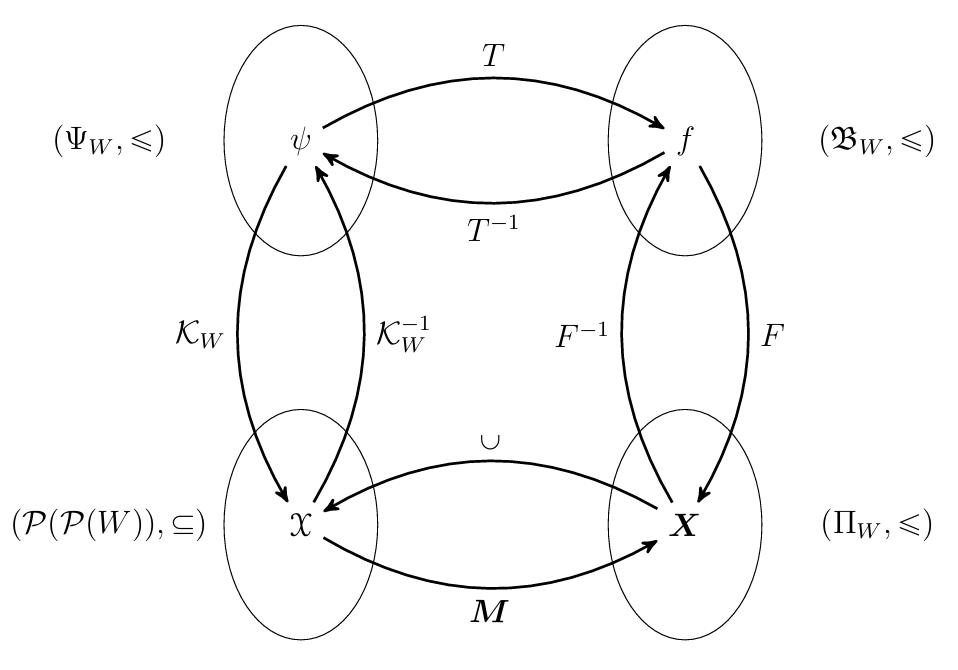
\includegraphics[width=0.75\textwidth]{figuras/lattice_isomorphism.png}
  \caption{Os isomorfismos de reticulados entre as representações dos W-operadores.\label{fig:isomorphism}}
\end{figure}

%%%%%%%%%%%%%%%%%%%%%%%%%%%%%%%%%%%%%%%%%%%%%%%%%%%%%%%%%%%%%%%%%%%%%%%%%%%%%%%%%%%%
\subsection{Projeto de W-operadores}
\label{subsec:compwop}

O projeto de W-operadores pode ser realizado por um processo de \textit{aprendizado computacional}, também conhecido como \textit{"Machine Learning"}, do tipo supervisionado, i.e., para cada exemplo observado, é fornecido também a classificação ou imagem transformada alvo do mesmo, ou seja, é dada uma coleção de pares de imagens binárias $\mathcal{S} \subseteq \mathcal{P} \left(E\right) \times \mathcal{P}\left(E\right)$, onde para todo $ \left( X,Y \right) \in \mathcal{S} $, $X$ é uma imagem que desejamos processar e $Y$ é a respectiva imagem ideal ou categoria de $X$ no caso de problemas de classificação (resultado que almejamos encontrar após o processamento de $X$). 

Esta abordagem consiste em um \textit{algoritmo de aprendizado} responsável por procurar uma função, também chamada de hipótese $h$, dentro de um espaço de hipóteses $\mathcal{H}$, i.e. $h \in \mathcal{H}$, capaz de transformar/classificar da melhor forma possível (ou com menor erro) os exemplos de treinamento. O espaço de hipóteses neste contexto é o espaço de todos os W-operadores $\Psi_{W}$ que podem ser representados pela composição de $n$ W-operadores com janelas conexas de um tamanho máximo pré-definido.

Em um processo de aprendizado buscamos sempre uma boa \textit{capacidade de generalização}. Um operador $\psi$ pode performar bem para o conjunto de imagens de treinamento $\left( X_{i},Y_{i} \right)$ (ou seja, $\psi \left( X_{i} \right) \approx Y_{i}$) e não ter uma boa generalização, performando mal para outros conjuntos de imagens $\left( X_{j},Y_{j} \right)$ (ou seja, $\psi \left( X_{j} \right) \neq Y_{j}$). Quando falamos em operador ideal ou operador ótimo em projeto de operadores, significa então encontrar um operador que tenha uma boa performance em qualquer par de imagens em um específico domínio, isto é, geradas por um mesmo processo.

Em termos estatísticos, podemos assumir que as imagens de entrada e saída são realizações de pares de conjuntos aleatórios discretos conjuntamente estacionários e cuja distribuição conjunta é caracterizada pelo W-operador com função característica $f_{\psi}: \mathcal{P} \left( W \right) \rightarrow \left\{ 0,1 \right\}$. Podemos considerar então que o processo local $S_{z} = X_{-z} \cap W = \left( X \cap W_{z} \right)_{-z} $ e $i_{z} = Y \left( z \right), z \in E, $ segue uma distribuição de probabilidade $P \left( S_{z}, \ i_{z} \right)$ fixada, mas desconhecida.

O operador $\psi$ é considerando um estimador de $Y$ com um erro de estimação definido em termos de uma função de perda $\ell: \psi \left( X \right) \times Y \to \mathbb{R}_{\geq0} $. O operador ótimo será aquele com menor erro dado pela perda esperada em qualquer posição $z$ por $R_{\ell} \langle \psi \rangle =  E_{P} \left[ \ell \left( f_{\psi} \left( S_{z} \right),i_{z} \right) \right]$, em que a esperança é em relação à distribuição $P$ que gerou os dados. Por exemplo, se a função de perda é a diferença absoluta $\ell \left(a,b \right)= \left| a-b \right|$ o erro esperado é o \textbf{MAE} - \textit{erro esperado médio} - em que fixada uma posição $z$, $MAE \langle \psi \rangle =E_{P} \left[ | f_{\psi} \left( S_{z} \right) - i_{z} | \right]$.

\begin{definition} 
        Dizemos que $\psi^{*} \in \Psi_{W} $ é ótimo em $\Psi_{W}$, segundo a função de perda $\ell$ se, e somente se  $R_{\ell} \langle \psi^{*} \rangle \leq R_{\ell} \langle \psi \rangle$, para todo $\psi \in \Psi_{W} $.
\end{definition}

Chamamos $R_{\ell} \langle \psi \rangle$ de \textit{out-of-sample error}, uma vez que o erro esperado é sob a distribuição $P$ que gerou os dados. Como $P$ é desconhecida, calculamos o erro empírico sob uma amostra de treinamento $\mathcal{D}_{N_{t}}$, onde $\mathcal{D}_{N_{t}} = \left\{ \left( X_{i}, Y_{i} \right) \ : \ 1 \leq i \leq N_{t} \right\}$ são $N_{t}$ pares $(X,Y)$ de imagens de entrada e de saída. Para cada operador $\psi \in \Psi_{W}$ definimos $L_{t}(\psi)$ como o seu erro empírico, ou \textit{in-sample-error}, que é a média amostral de $\sum\limits_{z} \ell \left( f_{\psi} \left( S_{z} \right),i_{z} \right)$.

É possível também incluir uma regularização implícita no processo de aprendizado através de uma amostra de validação $\mathcal{D}_{M}^{(val)}$, em que a amostra de treinamento é dividida de forma prévia e aleatória em duas, tal que, fixado um $M + N = N_{t}$ e , temos
$$\mathcal{D}_{N}^{(train)} = \left\{ (X_{i},Y_{i}): 1 \leq i \leq N \right\}$$
$$\mathcal{D}_{M}^{(val)} = \left\{ (X_{i},Y_{i}): N < i \leq N + M \right\}$$
Por simplificação, chamaremos a partir deste ponto $\mathcal{D}_{N}^{(train)}$ de $\mathcal{D}_{N}$ e $\mathcal{D}_{M}^{(val)}$ de $\tilde{\mathcal{D}}_{M}$, cujos erros empíricos (in-sample) denotamos por $L_{t}$ e $L_{v}$, respectivamente.

As instâncias na amostra de validação não estão nos dados de treinamento e assim fornecem informações com menor viés sobre a qualidade de generalização da hipótese selecionada. Assim realizaremos o aprendizado baseando-se nos dois erros $L_{t}$ e $L_{v}$.


%%%%%%%%%%%%%%%%%%%%%%%%%%%%%%%%%%%%%%%%%%%%%%%%%%%%%%%%%%%%%%%%%%%%%%%%%%%%%%%%%%%%
\subsection{Composição de W-operadores}
\label{subsec:compwop}

É possível obter um operador pela composição de operadores mais simples. Quando em um problema é necessário extrair diversas \textit{features} da imagem, como ruídos, filtragem de arestas ou segmentação de objetos, cada operador simples pode focar em um desses subproblemas e o operador final, que resolve o problema como um todo, é obtido pela composição sequencial desses operadores iniciais. 

Formalmente, seja $\theta = \left\{ \psi_{1}, ..., \psi_{n} \right\}, \ n \geq 2$, uma sequência de $n$ W-operadores com janelas $W_{1}, ...,  W_{n} $ e funções características $f_{1}, ..., f_{n}$. Definimos o W-operador multicamadas dado pela composição dos $n$ operadores em $\theta$ como
$$ \psi_{\theta} = \psi_{n} \circ \cdot \cdot \cdot \circ \psi_{1}. $$
O operador $\psi_{\theta}$ é \textit{i.t.} e \textit{l.d.} dentro da janela
$$W_{\theta} = W_{1} \oplus \cdot \cdot \cdot \oplus W_{n} $$
que seria a soma de Minkowski das $n$ janelas. 

Supondo que um operador $ \psi_{\theta} $ realize $n$ iterações sobre uma mesma janela $W$, temos então $n \times 2^{ \left| W \right|}$ parâmetros que precisam ser estimados, que são a imagem da função característica de cada operador. Já para um operador composto $\psi$ com janela $W^{\prime} = W_{1} \oplus \cdots \oplus W_{n}$, sendo $W_{i} = W$ para qualquer $i=1,...,n$, temos $2^{\left| W^{\prime} \right|}$ parâmetros. Por exemplo, se $W = W_{3 \times 3}$, $n = 2$ e $W^{\prime} = W \oplus W$, então $W^{\prime} = W^{\prime}_{5 \times 5}$ e para projetar o operador de 2 iterações sobre $W^{\prime}$ precisamos de $2 \times 2^{9} = 2^{10}$ parâmetros, enquanto para projetar diretamente o operador $\psi$ precisamos estimar $2^{25}$ parâmetros. Assim sendo, vemos que projetar um operador de forma composta possui muito menos parâmetros, o que indica que a sua precisão pode ser muito melhor que a precisão se projetássemos diretamente o operador final.

%%%%%%%%%%%%%%%%%%%%%%%%%%%%%%%%%%%%%%%%%%%%%%%%%%%%%%%%%%%%%%%%%%%%%%%%%%%%%%%%%%%%
\section{Espaço de Aprendizado}
\label{sec:ls}

O espaço de hipóteses $\mathcal{H}$ é um conjunto de hipóteses, que neste contexto serão W-operadores multicamadas. Um espaço $\mathcal{H}$ pode ser decomposto em sub-conjuntos chamados de modelos $\{\mathcal{M}_{1},\dots,\mathcal{M}_{k}\}, \mathcal{M}_{i} \subseteq \mathcal{H},$ de forma que
$$\mathcal{H} = \bigcup_{i=i}^{k} \mathcal{M}_{i}, $$
e uma possível abordagem de aprendizado nesse contexto seria primeiro selecionar um modelo dentre os candidatos, e então aprender uma hipótese nesse modelo.

Algoritmos tradicionais de \textit{seleção de modelos} buscam de forma exaustiva o melhor modelo baseado nos dados, primeiro encontrando a melhor hipótese em cada modelo, minimizando o erro em uma amostra de treinamento, e selecionando o modelo cuja hipótese encontrada minimiza o erro em uma amostra de validação.

Um Espaço de Aprendizado $\mathbb{L} \left( \mathcal{H} \right)$, também conhecido como \textit{Learning Space} (LS), é uma família de modelos candidatos parcialmente ordenados por inclusão, ou seja, um \textit{poset} de subespaços de $\mathcal{H}$, que pode ser projetada com conhecimento a priori e restrições específicas para cada classe de problemas. Além disso, alguns LS possuem uma estrutura com propriedades que podem ser aproveitadas na implementação de algoritmos não exaustivos de \textit{seleção de modelos} que, quando aliadados a alto poder computacional, permitem resolver problemas práticos que requerem algoritmos de alta complexidade \cite{DIEGO:01}. Abaixo definimos o LS. A dimensão VC de um espaço de hipóteses é uma medida da sua complexidade, cuja definição formal pode ser encontrada em \cite{DIEGO:01}.

\begin{definition} 
        Seja $\ell$ uma função de perda fixada e $\mathcal{H}$ um espaço de hipótese genérico com dimensão VC finita, $d_{VC} \left( \mathcal{H},\ell \right) < \infty	$. Seja $\mathbb{L} \left( \mathcal{H} \right):= \left\{ \mathcal{M}_{i} \ : \ i \in \mathcal{J} \subseteq \mathbb{Z}_{+}  \right\} $ um subconjunto finito do conjunto potência de $\mathcal{H}$, ou seja, $\mathbb{L} \left( \mathcal{H} \right) \subseteq \mathcal{P} \left( \mathcal{H} \right)$ e $ \left| \mathcal{J} \right| < \infty$. Dizemos que o \textit{poset} $ \left( \mathbb{L} \left( \mathcal{H} \right), \subseteq  \right)$ é um \textbf{Espaço de Aprendizado} sob a função de perda $\ell$ se,
        
        $ \left( i \right) \: \bigcup_{i \in \mathcal{J}} \mathcal{M}_{i} = \mathcal{H}$;
        
        $ \left( ii \right) \: \mathcal{M}_{1} , \mathcal{M}_{2} \in \mathbb{L} \left( \mathcal{H} \right) $ e $  \mathcal{M}_{1} \subseteq  \mathcal{M}_{2}$ implica em $d_{VC} \left( \mathcal{M}_{1},\ell \right) < d_{VC} \left( \mathcal{M}_{2},\ell \right) $

        Definimos a dimensão VC de $ \mathbb{L} \left( \mathcal{H} \right)$ como
        $$d_{VC} \left( \mathbb{L} \left( \mathcal{H} \right),\ell \right) := \max_{i \in \mathcal{J}}d_{VC} \left( \mathcal{M}_{i},\ell \right) $$
        cujo limite superior é $d_{VC} \left( \mathcal{H},\ell \right)$.
        \label{def:ls}
\end{definition}

Como $\mathbb{L} \left( \mathcal{H} \right)$ cobre $ \mathcal{H} $, quando buscamos um modelo em $\mathbb{L} \left( \mathcal{H} \right)$, nenhuma hipótese será descartada de antemão, mas uma restrição em $\mathcal{H}$ poderá ser aplicada somente a \textit{posteriori} e baseada nos dados.

Existem múltiplos subconjuntos de $\mathcal{P} \left( \mathcal{H} \right)$ que são LS, porém alguns subconjuntos, chamados de \textit{Lattice Learning Spaces}, possuem as propriedades de reticulado, que propiciam uma melhor eficiência nos algoritmos de seleção de modelo. O LS considerado neste trabalho faz parte dessa classe.

\begin{definition}
    Seja $\mathbb{L} \left( \mathcal{H} \right)$ um LS de $\mathcal{H}$. $\mathbb{L} \left( \mathcal{H} \right)$ será um \textbf{Lattice Learning Space} se $\left( \mathbb{L} \left( \mathcal{H} \right), \subseteq,\wedge,\vee, \mathcal{O}, \mathcal{I} \right)$ for um reticulado completo, que é um \textit{poset} com o menor $\left( \mathcal{O} \right)$ e maior $\left( \mathcal{I} \right)$ modelo, e com os operadores supremo $\vee$ e ínfimo $\wedge$ definidos para todos os subconjuntos de $\mathbb{L} \left( \mathcal{H} \right)$.
\end{definition}

\subsection{Cadeias Contínuas}

\textit{Cadeias Contínuas} no LS são cadeias sem saltos nos modelos em $\mathbb{L} \left( \mathcal{H} \right)$ quando consideramos a distância direta no grafo acíclico correspondente ao $\left( \mathbb{L} \left( \mathcal{H} \right),\subseteq \right)$, denotada por $d \left( \cdot , \cdot \right)$, conforme exemplificado na Figura \ref{fig:cadeia}.

\begin{definition}
    Uma sequência $\mathcal{M}_{i_{1}} \subseteq \mathcal{M}_{i_{2}} \subseteq \cdot \cdot \cdot \subseteq \mathcal{M}_{i_{k}} $ é chamada de \textbf{cadeia contínua} de $\mathbb{L} \left( \mathcal{H} \right)$ se, e somente se,
    $$d \left( \mathcal{M}_{i_{j}},\mathcal{M}_{i_{j+1}} \right) = 1 \; \text{para todo } j \in \left\{ 1,...,k-1 \right\}$$ 
\end{definition}

\begin{figure}
  \centering
  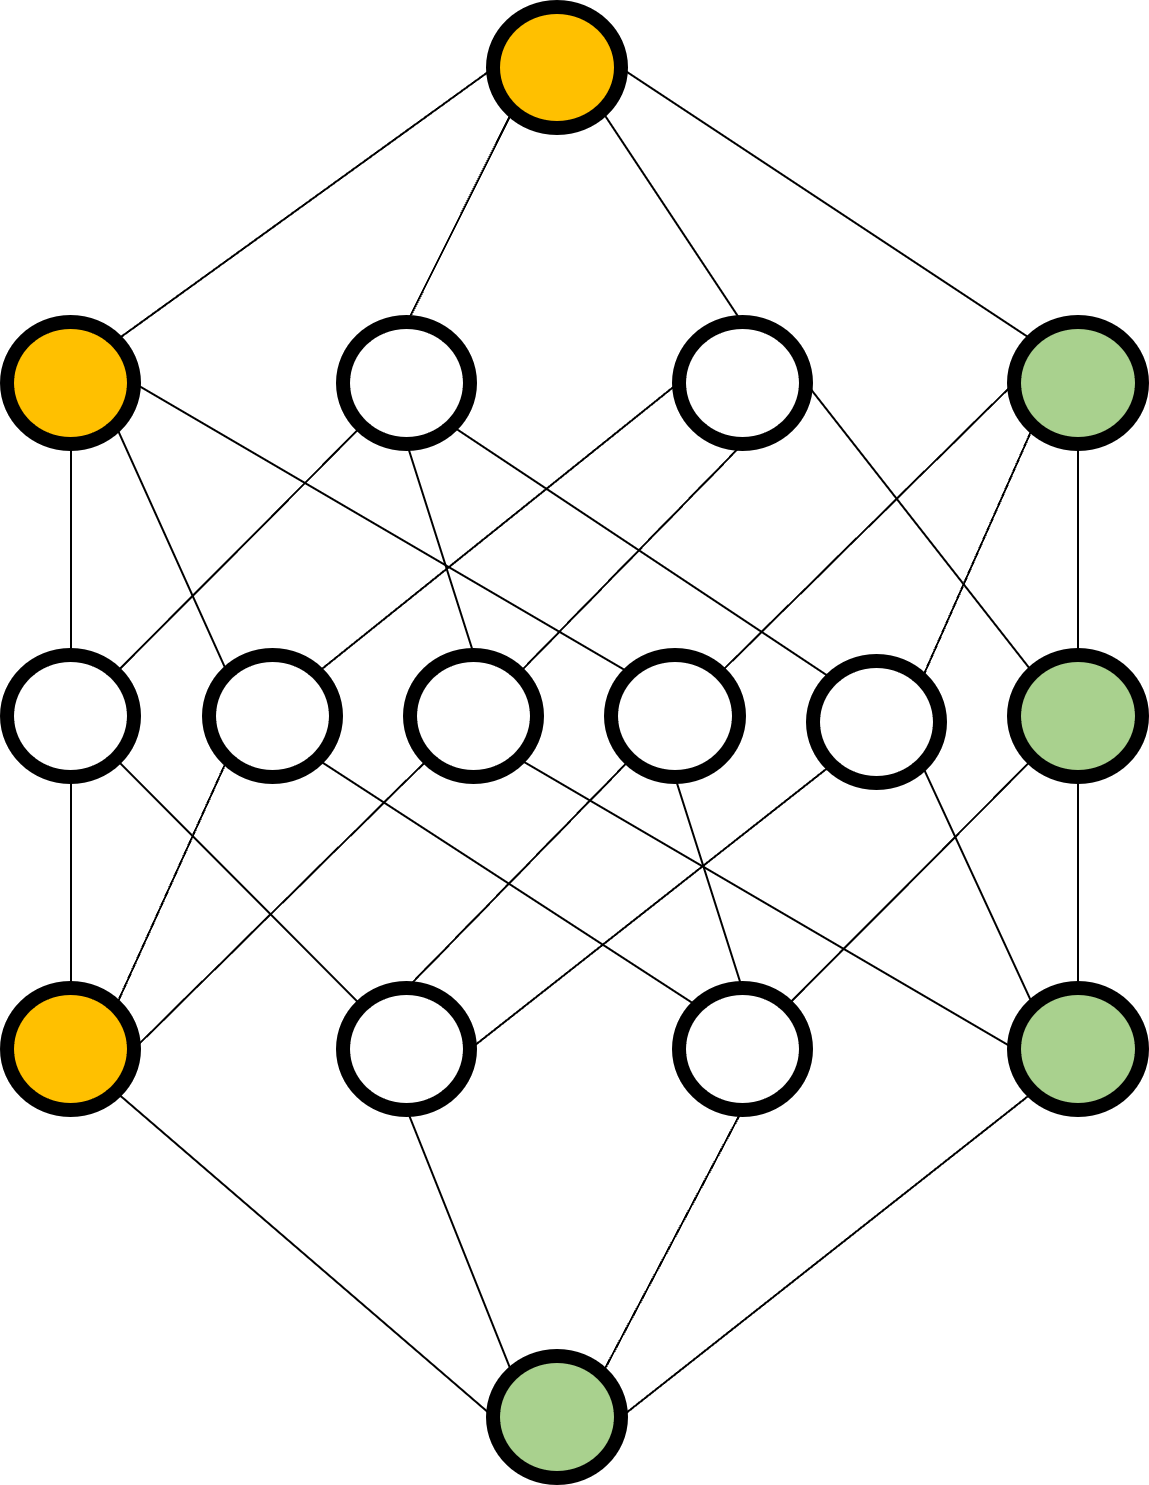
\includegraphics[width=.4\textwidth]{figuras/cadeia.png}
  \caption{Exemplo de uma cadeia contínua (verde) e uma cadeia não contínua (amarelo) em um LS Booleano.\label{fig:cadeia}}
\end{figure}

\subsection{Mínimos no Espaço de Aprendizado}

Seleção de modelos via LS depende do conceito de \textit{mínimos} de um $\mathbb{L} \left( \mathcal{H} \right)$ quando o erro de um modelo $\mathcal{M}$ é estimado por um estimador fixo $\hat{L} \left( \mathcal{M} \right)$.

\begin{definition}
    O modelo $\mathcal{M}_{i_{j^{*}}}$ é,
    \begin{itemize}
        \item Um \textbf{mínimo local fraco} de uma cadeia contínua  $\mathcal{M}_{i_{1}} \subseteq \mathcal{M}_{i_{2}} \subseteq \cdot \cdot \cdot \subseteq \mathcal{M}_{i_{k}} $ de $\mathbb{L} \left( \mathcal{H} \right)$ se
        $$\hat{L} \left( \mathcal{M}_{i_{j^{*}}} \right) \leq \min \left( \hat{L} \left( \mathcal{M}_{i_{j^{*}-1}} \right), \hat{L} \left( \mathcal{M}_{i_{j^{*}+1}} \right)  \right)$$
        onde $\hat{L} \left( \mathcal{M}_{i_{0}} \right) \equiv \hat{L} \left( \mathcal{M}_{i_{k+1}} \right) \equiv + \infty  $ ;

        \item Um \textbf{mínimo local forte} de $\mathbb{L} \left( \mathcal{H} \right)$ é um mínimo local fraco de todas as cadeias contínuas de $\mathbb{L} \left( \mathcal{H} \right)$ que o contém, ou seja,
        $$\hat{L} \left( \mathcal{M}_{i_{j^{*}}} \right) \leq \min \left\{ \hat{L} \left( \mathcal{M} \right) \ : \ \mathcal{M} \in \mathbb{L} \left( \mathcal{H} \right), \ d \left( \mathcal{M}_{i_{j^{*}}}, \mathcal{M} \right) = 1 \right\} \text{;}$$

        \item Um \textbf{sup-mínimo local fraco} de $\mathbb{L} \left( \mathcal{H} \right)$ se,
        $$\hat{L} \left( \mathcal{M}_{i_{j^{*}}} \right) \leq \min \left\{ \hat{L} \left( \mathcal{M} \right) \ : \ \mathcal{M} \in \mathbb{L} \left( \mathcal{H} \right), \ \mathcal{M}_{i_{j^{*}}} \subseteq \mathcal{M} \ ,\ d \left( \mathcal{M}_{i_{j^{*}}}, \mathcal{M} \right) = 1 \right\} \text{;}$$

        \item Um \textbf{inf-mínimo local fraco} de $\mathbb{L} \left( \mathcal{H} \right)$ se,
        $$\hat{L} \left( \mathcal{M}_{i_{j^{*}}} \right) \leq \min \left\{ \hat{L} \left( \mathcal{M} \right) \ : \ \mathcal{M} \in \mathbb{L} \left( \mathcal{H} \right), \ \mathcal{M} \subseteq \mathcal{M}_{i_{j^{*}}} \ ,\ d \left( \mathcal{M}_{i_{j^{*}}}, \mathcal{M} \right) = 1 \right\} \text{;}$$

        \item Um \textbf{mínimo global} de uma cadeia contínua se,
        $$ \hat{L}  \left( \mathcal{M}_{i_{j^{*}}} \right) = \min_{1 \leq j \leq k} \hat{L}  \left( \mathcal{M}_{i_{j}} \right) \text{;}$$

        \item Um \textbf{mínimo global} de $\mathbb{L} \left( \mathcal{H} \right)$ se,
        $$ \hat{L}  \left( \mathcal{M}_{i_{j^{*}}} \right) = \min_{1 \in \mathcal{J}} \hat{L}  \left( \mathcal{M}_{i_{j}} \right) \text{.}$$
        
    \end{itemize}
    \label{def:minimos}
\end{definition}

\subsection{O Aprendizado de Hipóteses via Espaço de Aprendizado}

O \textit{framework} de LS para aprender hipóteses é composto de dois passos:

\begin{enumerate}
    \item Aprender um modelo $\hat{\mathcal{M}}$ em $\mathbb{L} \left( \mathcal{H} \right)$ pela minimização da medida de erro $\hat{L}$. Formalmente, sendo    
    $$\hat{\mathcal{L}} =  \underset{\mathcal{M}\in \mathbb{L}\left( \mathcal{H}\right)}{\arg \min} \  \hat{L} \left( \mathcal{M} \right)$$
    os modelos que minimizam $\hat{L}$ em $\mathbb{L}(\mathcal{H})$, aprendemos   
   $$\hat{\mathcal{M}} =  \underset{\mathcal{M}\in \hat{\mathcal{L}}}{\arg \min} \  d_{VC} \left( \mathcal{M} \right)$$
   que é o modelo mais simples dentre os mínimos globais.

   \item Aprender uma hipótese em $\hat{\mathcal{M}}$ pela minimização do erro empírico $L_{t}$ em uma amostra $\mathcal{D}_{N}$. Formalmente, a hipótese aprendida será
   $$ \hat{h}_{\hat{\mathcal{M}}}^{\mathcal{D}_{N}} := \underset{h \in \hat{\mathcal{M}}}{\arg \min} \ L_{D_{N}} \left( h \right)$$
\end{enumerate}


%%%%%%%%%%%%%%%%%%%%%%%%%%%%%%%%%%%%%%%%%%%%%%%%%%%%
\section{U-curve no Espaço de Aprendizado}
\label{sec:ucurve}

Quando modelos são organizados em estruturas de reticulado, apesar de frequentemente não termos a prova matemática, temos evidências empíricas do comportamento heurístico de propriedade de U-curve no LS. As propriedades U-curve são uma das poucas que garantem rigorosamente uma solução ótima sem a necessidade de uma busca exaustiva de todos os modelos candidatos no espaço de aprendizado. Mesmo quando a propriedade não é totalmente satisfeita, ou comprovada, é possível utilizar-se dela e encontrar uma solução sub-ótima aceitável.

Um exemplo do fenômeno de U-curve se dá conforme caminhamos em uma cadeia de modelos $\mathcal{M}_{0} \subseteq \cdot \cdot \cdot \subseteq \mathcal{M}_{6}$ onde a complexidade (em termos de dimensão VC) vai aumentando, sendo $\mathcal{M}_{0}$ menos complexo e $\mathcal{M}_{6}$ mais complexo. A princípio o erro estimado $\hat{L}$ diminui até encontrar um ponto de inflexão e começar a monotonicamente crescer com o aumento da complexidade, conforme ilustrado na Figura \ref{fig:ucurve}. Este fenômeno, quando atrelado ao aumento do número de variáveis e/ou parâmetros dos modelos, é conhecido como fenômeno de pico (\textit{peaking phenomenon}), conforme ilustrado em \cite{ucurve:06,ucurve:01, ucurve:02, ucurve:03, ucurve:05, ucurve:04}.

\begin{figure}
  \centering
  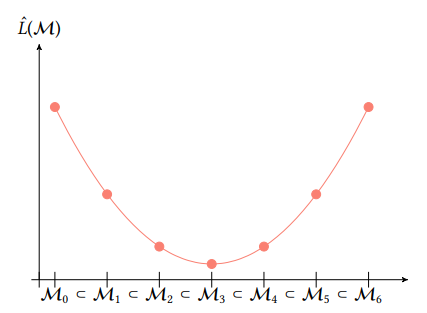
\includegraphics[width=.4\textwidth]{figuras/u_curve.png}
  \caption{Ilustração do fenômeno de U-curve apresentada por \cite{DIEGO:01} em uma cadeia de modelos com aumento de complexidade.\label{fig:ucurve}}
\end{figure}

 
 %\subsection{Propriedades de U-curve}
 Podemos definir as \textbf{Propriedades de U-curve} baseando-se nas Definições em \ref{def:minimos} e no estimador $\hat{L}$.

 \begin{definition}
     Um LS $\mathbb{L} \left( \mathcal{H} \right)$ sob uma função de perda $\ell$ e um estimador $\hat{L}$ satisfaz:

     \begin{itemize}
         \item \textbf{Propriedade U-curve Forte} se todos os mínimos locais fracos de uma cadeia contínua de $\mathbb{L} \left( \mathcal{H} \right)$ são um mínimo global dessa cadeia;

         \item \textbf{Propriedade U-curve Fraca} se todos os mínimos locais fortes são um mínimo global de todas as cadeias contínuas de $\mathbb{L} \left( \mathcal{H} \right)$ que o contém;

         \item \textbf{Propriedade U-curve Sup-Fraca} se todos os sup-mínimos locais fortes possuem um erro estimado menor ou igual ao de todos os modelos em $\mathbb{L} \left( \mathcal{H} \right)$ que o contém;

         \item \textbf{Propriedade U-curve Inf-Fraca} se todos os inf-mínimos locais fortes possuem um erro estimado menor ou igual ao de todos os modelos em $\mathbb{L} \left( \mathcal{H} \right)$ que o contém;
     \end{itemize}

     As condições que caracterizam as propriedades de U-curve devem ser verdade com probabilidade 1, válida para todas as possíveis amostras sob as quais $\hat{L}$ é calculada.
 \end{definition}


Podemos aproveitar as propriedades U-curve em um algoritmo de minimização de $\hat{L}$ para evitar uma busca exaustiva de $\mathbb{L} \left( \mathcal{H} \right)$. 
 
Caso a propriedade U-curve Forte seja satisfeita, o Algoritmo U-curve deve percorrer todas as cadeias contínuas de $\mathbb{L} \left( \mathcal{H} \right) $ até encontrar o seu (único) mínimo local fraco, de modo que encontremos todos os mínimos locais fracos e, portanto, o mínimo global. Similarmente, caso a propriedade U-curve Fraca seja satisfeita, o Algoritmo U-curve deve percorrer todas as cadeias contínuas de $\mathbb{L} \left( \mathcal{H} \right) $ até encontrar o seu (único) mínimo local forte, de modo que encontremos todos os mínimos locais fortes e, portanto, o mínimo global. Nos dois cenários, $\mathbb{L} \left( \mathcal{H} \right) $ não é percorrido exaustivamente, pois uma vez que encontramos um mínimo local forte ou fraco não precisamos calcular o erro dos modelos restantes da cadeia.

Por outro lado, se a propriedade U-curve Sup-Fraca (ou Inf-Fraca) for satisfeita, podemos percorrer todas as cadeias contínuas de $\mathbb{L} \left( \mathcal{H} \right) $ até encontrarmos um sup-mínimo (inf-mínimo) local forte e, portanto, o mínimo global. Neste caso $\mathbb{L} \left( \mathcal{H} \right) $ também não é percorrido exaustivamente, pois quando encontramos um sup-mínimo (inf-mínimo) local forte não precisamos calcular o erro dos modelos maiores (menores) da cadeia contínua.

Por fim, quando as propriedades U-curve não são estritamente satisfeitas e ainda assim utilizarmos o Algoritmo U-curve, teremos uma solução sub-ótima, uma vez que podemos perder o mínimo global quando não visitamos o restante dos modelos da cadeia ao encontrar o seu respectivo mínimo local. Ainda assim o algoritmo pode retornar um mínimo local com baixo erro e ser suficiente para a aplicação prática em questão.
%!TeX root=../tese.tex
%("dica" para o editor de texto: este arquivo é parte de um documento maior)
% para saber mais: https://tex.stackexchange.com/q/78101

\chapter{Modelo de Aprendizado}
\label{chap:modelo}

O objetivo deste capítulo é apresentar as definições dos modelos de aprendizado de W-operadores multicamadas (WOMC) nos contextos de transformação de imagens e para classificação de imagens, de acordo com o modelo proposto por \cite{DIEGO:01}, que serão a base de desenvolvimento deste trabalho.


\section{W-operadores Multicamadas para Transformação de Imagens}
\label{sec:Wop_transformacao}

No contexto de transformação de imagens, os WOMC são uma composição de $n$ W-operadores aplicados em sequência a uma imagem de entrada $X \in \mathcal{P}\left( E \right)$ conforme apresentado em \ref{subsec:compwop}.

A família de W-operadores considerada neste trabalho é caracterizada por janelas com dimensão máxima fixada. Seja $d_{W} \geq 3$ um número ímpar e $F_{d_{W}} = \left\{ - \left( d_{W} -1 \right) /2 ,..., \left(	d_{W} - 1 \right) /2 \right\}^{2} $ o quadrado de lado $d_{W}$ centrado na origem de $E$. Nós consideramos que a janela $W$ de cada W-operador de um WOMC é um subconjunto de $F_{d_{W}}$, com a restrição de ser um conjunto conectado, ou seja, para cada $w, w' \in W$ existe uma sequência $w_{0},...,w_{r} \in W, \ r \geq 1, $ tal que $w_{0} = w, \ w_{r} = w' $ e 
$$ \| w_{i} - w_{i+1} \|_{\infty} = 1, \text{ para todo } i=0,...,r-1. $$
Formalmente, $W \in \mathscr{C}$ em que
$$ \mathscr{C} = \left\{ W \subseteq F_{d_{W}}  : W \text{ é conectado} \right\}. $$
Na figura \ref{fig:wconect} apresentamos exemplos de janelas que estão e não estão em $\mathscr{C}$.

\begin{figure}
  \centering

  \begin{subfigure}{0.4\textwidth}
    \centering
    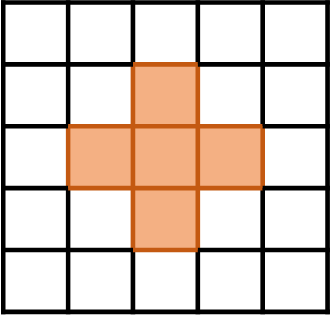
\includegraphics[width=.8\textwidth]{figuras/W_conectada.png}
    \caption{Janela $W \in \mathscr{C}$ - Conectada\label{fig:subfig:wconect}}
  \end{subfigure}
  \begin{subfigure}{0.4\textwidth}
    \centering
      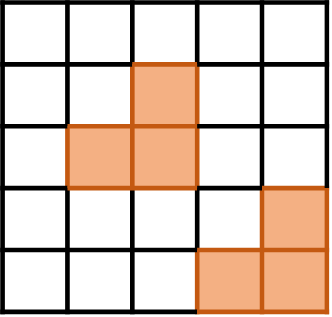
\includegraphics[width=.8\textwidth]{figuras/W_nconectada.png}
    \caption{Janela $W \notin \mathscr{C}$ - Desconectada.\label{fig:subfig:wnotconect}}
  \end{subfigure}

  \caption{Exemplo de Janelas contida em $F_{5}$ que respeita (esquerda) e não respeita (direita) a restrição de W-operadores de ser conectada.\label{fig:wconect}}
\end{figure}

Para cada $W \in \mathscr{C} $, defina o conjunto de todas as funções binárias com domínio $\left\{ 0,1 \right\}^{W} $ como
$$ \mathcal{F}_{W} = \left\{ f: \left\{ 0,1 \right\}^{W} \mapsto \left\{ 0,1 \right\} \right\}. $$
Definimos a coleção de W-operadores com janela em $ \mathscr{C}$, que são completamente definidos por $W \in \mathscr{C} $ e $f \in \mathcal{F}_{W}$, como
$$\mathcal{F} = \left\{ \left( W,f \right) : W \in \mathscr{C}, \ f \in \mathcal{F}_{W} \right\}. $$
Por fim, o produto cartesiano das $n$ cópias de $\mathcal{F}$ pode ser definido como
$$\Theta = \prod_{i=1}^{n} \mathcal{F}, $$
e um elemento $\theta$ em $\Theta$ será então uma sequência de $n$ W-operadores com janelas em $\mathscr{C}$ denotada por
$$ \theta := \left\{ \left(W_{1}, f_{\psi_{1}} \right), \cdot \cdot \cdot, \left(W_{n}, f_{\psi_{n}} \right) \right\}$$

Para cada $\theta \in \Theta$ temos o WOMC 
\begin{equation}
    \psi_{\theta} := \left( \psi_{n} \circ \cdot \cdot \cdot \circ \psi_{1}  \right).
    \label{eq:multicamadas_1}
\end{equation}
Um WOMC no contexto de transformação de imagens pode ser visto como um pipeline de transformação de imagens no qual cada W-operador executa sequencialmente uma transformação em uma imagem de entrada $X$, e uma imagem transformada $Y = \psi_{\theta} \left( X \right) $ é obtida. 

O Espaço de Hipóteses dos WOMC para a transformação de imagens será então
$$\mathcal{H} := \left\{ \psi_{\theta} : \theta \in \Theta \right\}. $$


%%%%%%%%%%%%%%%%%%%%%%%%%%%%%%%%%%%%%%%%%%%%%%%%%%%%%%%%%%%%%%%%%%%%%%%%%%

\section{W-operador Multicamadas para Classificação de Imagens}

WOMC também podem ser utilizados no contexto de classificação de imagens binárias, onde a \textit{transformação} da imagem de entrada deve levar a uma classificação ao invés de uma imagem transformada. Para isso, podemos considerar a composição de \textit{W-operadores emoldurados}, onde após a aplicação de cada operador, a imagem perde dimensões, e ao final da pipeline obtemos um número em $\left\{ 0,1 \right\}$.

\subsection{W-operadores Emoldurados}

Seja $F_{1} = \left\{ \left( 0,0 \right) \right\}$ a origem de $E = \mathbb{Z}^{2}$ e para $p \geq 3$, ímpar, seja
$$F_{p} = \left\{ - \left(p-1 \right) /2 , ... , \left( p-1 \right) /2 \right\}^{2} \subseteq E $$
o conjunto de pontos em $E$ que formam um quadrado de $p^{2}$ pontos centrados na origem. Chamamos de $F_{p}$ a moldura de tamanho $p$. Uma imagem está emoldurada em $F_{p}$ se
$$X \subseteq F_{p}.$$
Se $X$ está emoldurado em $F_{p}$, então $X$ pode ser representado como uma imagem com $p \times p$ pixels.

Ao analisar $X$, e interpretando um W-operador como centralizando a janela $W$ em cada ponto em $z \in F_{p}$ e assumindo $z \in \psi \left( X \right)$ baseado em $f_{\psi} \left( X \cap W_{z} \cap F_{p} \right)$, podemos observar que, na verdade, não podemos centralizar a janela $W$ em todos os pontos de $F_{p}$, uma vez que $W$ não está contida em $F_{p}$ se estiver centrada em pontos próximos às bordas da imagem.

A proximidade das bordas pode ser definida em termos de uma moldura que contém $W$, assumindo que $W \subseteq F_{d_{W}}, \ d_{W} \geq 3$ ímpar, ou seja, a janela $W$ é um subconjunto da moldura $d_{W}$ com $d_{W} \leq p$. Então, podemos definir o W-operador emoldurado associado a $\psi \in \Psi_{W}$ como
\begin{equation}
    \psi_{p,d_{W}}^{fr} \left( X \right) = \psi \left( X \right) \cap F_{p-(d_{W}-1)}
    \label{eq:wemoldurado}
\end{equation}
para qualquer $X \subseteq F_{p}$, que é obtido ao centralizar a janela $W$ apenas em pontos $z \in F_{p}$ no qual $ \left[ F_{d_{W}} \right]_{z} \subseteq F_{p} $, ou seja, a moldura de $W$ está completamente contida na moldura de $X$. A Figura \ref{fig:dig0jan1} apresenta um exemplo de W-operador emoldurado.

Quando $\psi_{p,d_{W}}^{fr}$ é aplicado a uma imagem emoldurada em $F_{p}$ a imagem resultante perderá $\left( d_{W}-1 \right)$ linhas e colunas, contendo $p- \left( d_{W}-1 \right) \times p- \left( d_{W}-1 \right)$ pixels e estará emoldurada em $ F_{p-(d_{W}-1)}$, portanto
$$\psi_{p,d_{W}}^{fr} : \mathcal{P} \left( F_{p} \right) \to  \mathcal{P} \left( F_{p-(d_{W}-1)} \right). $$

\begin{figure}
    \centering
    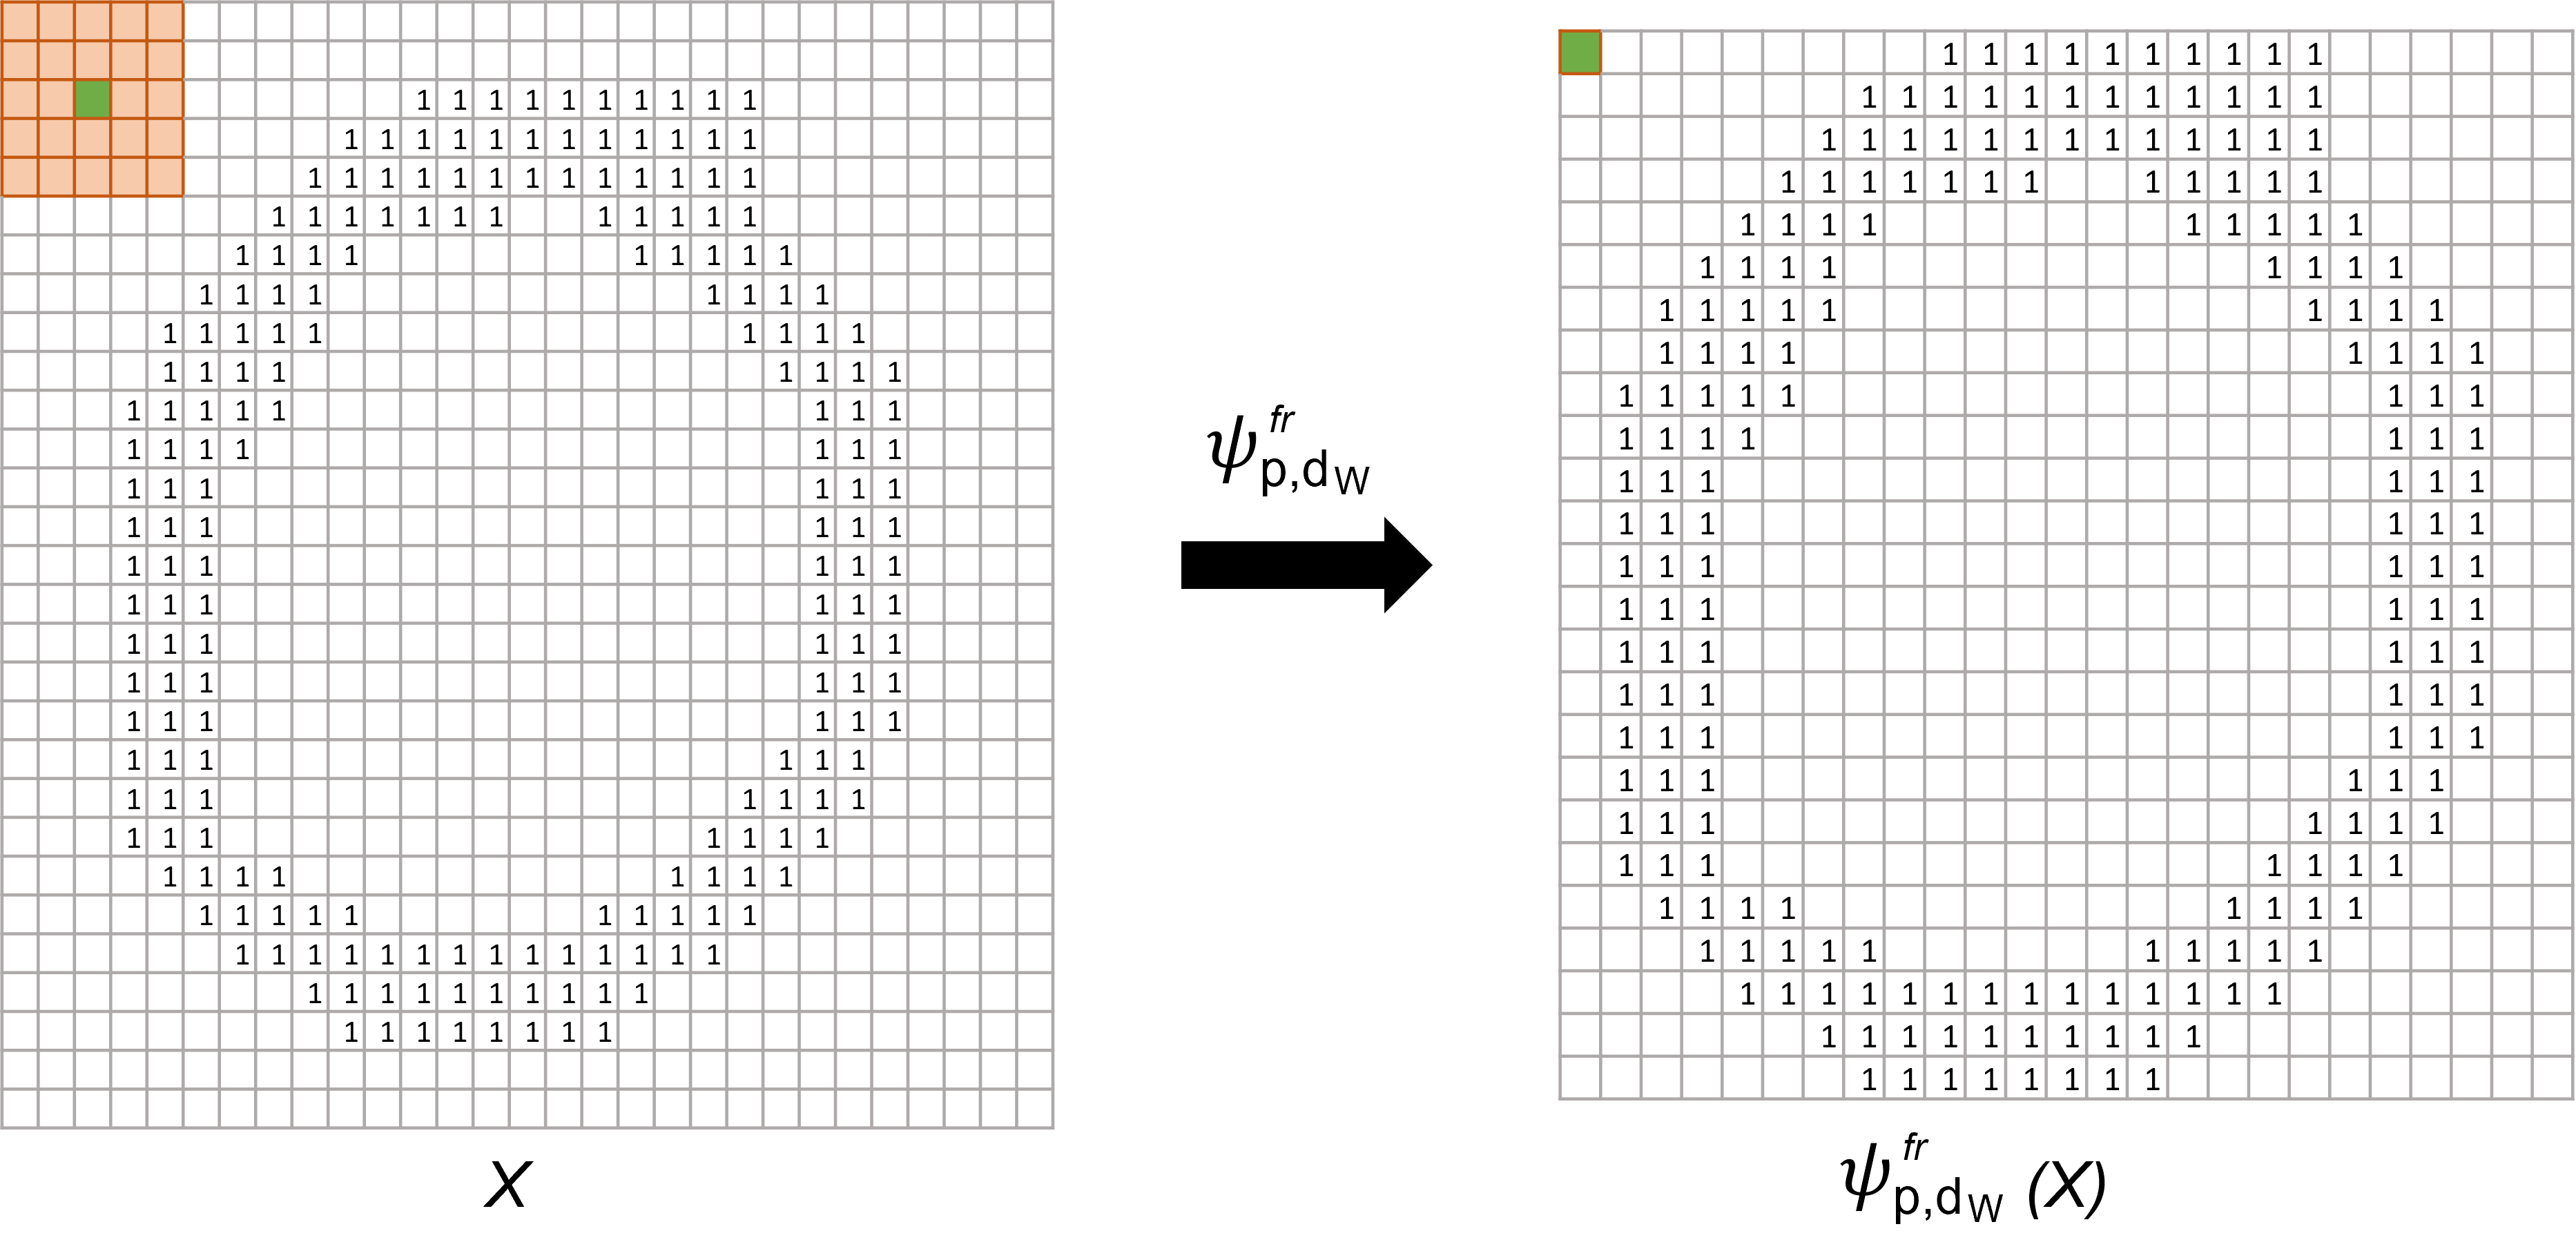
\includegraphics[scale = 0.5]{figuras/digito0_janela1_framed.png}
    \caption{Exemplo de um W-operador emoldurado $ \psi_{p,d_{W}}^{fr}$ com janela $W_{1} \subseteq F_{5}$ em laranja, na imagem $X$ a esquerda, centrado no primeiro pixel possível em verde. A imagem $ \psi_{p,d_{W}}^{fr} \left( X \right)$, obtida após aplicação do operador identidade, encontra-se a direita, com redução de dimensionalidade, indicando o pixel correspondente ao primeiro pixel de $X$ também em verde.}
    \label{fig:dig0jan1}
\end{figure}

\subsection{Classificação}

Considerando os W-operadores emoldurados definidos em \eqref{eq:wemoldurado} observamos que, como a cada aplicação de um W-operador emoldurado perdemos $d_{w} - 1$ dimensões, se aplicarmos
$$n = \left( p - 1 \right) / \left( d_{W} - 1 \right)$$
W-operadores emoldurados obteremos uma imagem com apenas um pixel, assumindo que $n \in \mathbb{Z}$ e $n \geq 2$. Dessa forma, a aplicação de $n$ W-operadores emoldurados gerará um classificador de $\mathcal{P}(F_{p})$ em $\mathcal{P}(F_{1}) \simeq \{0,1\}$.

Para cada $ \theta = \left\{ \left(W_{1}, f_{1} \right), ..., \left(W_{n}, f_{n} \right) \right\} 
\in \Theta $, seja $ \theta_{fr} = \left\{ \psi_{1}^{fr},..., \psi_{n}^{fr} \right\}$ a sequência de W-operadores emoldurados dados por
$$\psi_{i}^{fr}:= \left( \psi_{i} \right)_{p-(i-1)(d_{W}-1),d_{W}}^{fr} \left( X \right) = \psi_{i} \left(X \right) \cap F_{p-i(d_{W}-1)} $$
para $X \subseteq F_{p-(i-1)(d_{W}-1)}$, em que $\psi_{i}$ é o W-operador com janela $W_{i}$ e função característica $f_{i}$ para $i=1,...,n$. Compondo essa sequência de W-operadores emoldurados obtemos o classificador
\begin{equation}
    \label{eq:emolduradas}
    h_{\theta} = \psi_{n}^{fr} \circ \cdot \cdot \circ \psi_{1}^{fr} 
\end{equation}
que é uma função de $\mathcal{P}\left(F_{p} \right) $ para $\mathcal{P}\left(F_{1} \right) \simeq \left\{ 0,1 \right\}$. Chamamos $h_{\theta}$ para $\theta \in \Theta$ um \textit{W-operador multicamada para classificação de imagens}.

\subsection{Ideias Principais e Definições na Classificação de Dígitos}
\label{subsec:ideias}

O problema de aprendizado de reconhecimento de dígitos, busca um classificador no qual dado uma imagem, o retorno do classificador será 1 se o dígito em questão, por exemplo, o dígito 0, estiver na imagem e 0 caso contrário. Uma imagem binária contendo o dígito 0 pode ser vista como uma matriz de pixels brancos e pretos onde o branco terá o valor 0 e preto terá o valor 1 conforme exemplificado na Figura \ref{fig:dig_0} . 

\begin{figure}
    \centering
    
\includegraphics[width=.4\textwidth]{figuras/digito_0.png}
    \caption{Exemplo de matriz de uma imagem binária com dígito 0 onde os pixels pretos são representados por 1 e os pixels brancos são representados por 0. Os valores zero foram omitidos para uma melhor visualização.}
    \label{fig:dig_0}
\end{figure}

O problema de reconhecimento de dígitos possui naturalmente uma restrição de ser invariante por translação, uma vez que a classificação do dígito não deve depender de sua posição na imagem, por exemplo, se ele estiver centralizado ou deslocado do centro. Esta e outras restrições são feitas implicitamente pela representação paramétrica das hipóteses como WOMC para classificação de imagens de forma que o Espaço de Hipóteses é
$$\mathcal{H} = \left\{ h_{\theta} : \theta \in \Theta \right\}$$
sendo $h_{\theta} $ a hipótese com parâmetro $\theta \in \Theta$ definida por \eqref{eq:emolduradas}.

Por exemplo, assumindo que as imagens com os dígitos possuem tamanho $29 \times 29$, ou seja, $p = 29$ e $X \subseteq F_{29}$, e a janela $W$ tem tamanho $5 \times 5$, ou seja, $d_{W} = 5$ e $W \subseteq F_{5}$, temos que $n = 7$ e
$$ \theta_{fr} = \left\{ \left(W_{1}, f_{\psi_{1}^{fr}} \right), \cdot \cdot \cdot, \left(W_{7}, f_{\psi_{7}^{fr}} \right) \right\}$$
representará uma sequência fixa de sete W-operadores que gera o classificador
$$h_{\theta} := \left( \psi_{7}^{fr} \circ \psi_{6}^{fr} \circ \psi_{5}^{fr} \circ \psi_{4}^{fr} \circ \psi_{3}^{fr} \circ \psi_{2}^{fr} \circ \psi_{1}^{fr}  \right).$$

Então, após aplicar cada W-operador a dimensão da saída reduz em $4$ unidades e como $28 = p-1 = n \left( d_{W}-1 \right) = 7 \times 4$, após aplicar $7$ W-operadores em sequência, a dimensão da saída será $p - n \left( d_{W}-1 \right) = 29 - 28 = 1$, e $h_{\theta}$ terá imagem em $\left\{ 0,1 \right\}$. 


%%%%%%%%%%%%%%%%%%%%%%%%%%%%%%%%%%%%%%%%%%%%%%%%%%%%%%%%%%%%%%%%%%%%%%%%%%%%%%%%%%%
\section{Aprendizado de W-operadores Multicamadas}
\label{sec:aprendizado}

O aprendizado de W-operadores multicamadas no contexto de transformação ou de classificação de imagens é semelhante e será apresentado nesta seção. O algoritmo aprende de forma simultânea a janela e a função característica de todos os W-operadores.

\subsection{Amostras de Treino e Validação}

Para um valor fixo $p \in \mathbb{Z}_{+} $, seja $\mathcal{D}_{N} = \left\{ \left( X_{1}, Y_{1} \right),...,\left( X_{N}, Y_{N} \right) \right\} $ a amostra de treinamento de $N$ imagens de entrada emolduradas $X_{i} \subseteq F_{p} $ e suas correspondentes imagens de saída $Y_{i} \subseteq F_{q} $. No contexto de transformação de imagens assumimos que $q = p$ de forma que $Y_{i} \subseteq F_{p} $ é uma imagem emoldurada obtida pela transformação de $X_{i}$. Já no contexto de classificação de imagens assumimos que $q=1$ e $Y_{i} \in \mathcal{P} \left( \left\{ \left( 0,0 \right) \right\} \right) \simeq \left\{ 0,1 \right\} $ é a classe de $X_{i}$.

Quando $ Y_{i}, \ i = 1,...,N,$ são imagens emolduradas em $F_{p}$, denotamos para $ \left( j,k \right) \in F_{p} $ e $\theta \in \Theta$ como
$$\left( Y_{i} \right)_{j,k}$$
o valor do pixel $\left( j,k \right)$ na imagem $Y_{i}$ e 
$$ \left( \psi_{\theta} \left( X_{i} \right) \right)_{j,k} $$
o valor do pixel $\left( j,k \right)$ na imagem $\psi_{\theta} \left( X_{i} \right)$.

Seja $ \ell \left( \left( X_{i}, Y_{i} \right), \theta \right) \in \mathbb{R}_{+}$ o erro obtido quando o W-operador $ \psi_{\theta}$  é aplicado para transformar $X_{i}$ em $Y_{i}$, ou quando o classificador $h_{\theta}$ é utilizado para prever a classe $Y_{i}$ de $X_{i}$. Neste trabalho consideramos duas funções de perda quando $Y_{i}$ é uma imagem emoldurada em $F_{p}$, \textbf{MAE} dada por
$$ \ell_{MAE} \left( \left( X_{i}, Y_{i} \right), \theta \right) = \frac{1}{p^{2}} \sum_{(j,k) \in F_{p}} | \left( \psi_{\theta} \left( X_{i} \right) \right)_{j,k} - \left( Y_{i} \right)_{j,k} | $$
ou interseção sobre união (\textbf{IoU}) dada por
$$ \ell_{IoU} \left( \left( X_{i}, Y_{i} \right), \theta \right) = 1 - \frac{Y_{i} \cap \psi_{\theta} \left( X_{i} \right)}{Y_{i} \cup \psi_{\theta} \left( X_{i} \right)} $$
quando $Y_{i}$ é uma classe de $X_{i}$, utilizamos o erro \textbf{MAE} dado por
$$ \ell_{MAE} \left( \left( X_{i}, Y_{i} \right), \theta \right) = | h_{\theta} \left( X_{i} \right) - Y_{i} |. $$
O erro empírico de $\theta \in \Theta$ na amostra de treinamento $\mathcal{D}_{N}$ será então considerado como
$$ L_{t} \left( \theta \right) = \frac{1}{N} \sum_{i=1}^{N} \ell  \left( \left( X_{i}, Y_{i} \right), \theta \right). $$

No contexto de transformação de imagens, $L_{t}$ representa a proporção média de pixels com valores distintos em $Y_{i}$ e $\psi_{\theta} \left( X_{i} \right), \ i=1,...,N $ e, no contexto de classificação de imagens, $L_{t}$ representa o erro de classificação de $h_{\theta}$ na amostra $\mathcal{D}_{N}$.

Analogamente, temos a amostra de validação $\tilde{\mathcal{D}}_{M} = \left\{ \left( \tilde{X}_{1}, \tilde{Y}_{1} \right),...,\left( \tilde{X}_{M}, \tilde{Y}_{M} \right) \right\} $, que é independente de $\mathcal{D}_{N}$, cujo erro empírico é dado por
$$ L_{v} \left( \theta \right) = \frac{1}{M} \sum_{i=1}^{M} \ell  \left( \left( \tilde{X}_{i}, \tilde{Y}_{i} \right), \theta \right) $$
para $\theta \in \Theta$.

A partir deste ponto não faremos distinção entre o aprendizado de WOMC nos contextos de transformação e classificação de imagens, uma vez que são análogos, com a diferença no cálculo do erro empírico, conforme apresentado acima.

%%%%%%%%%%%%%%%%%%%%%%%%%%%%%%%%%%%%%%%%%%%%%%%%%%%%%%
\subsection{LS para o Aprendizado de W-operadores Multicamadas}

Para cada sequência de $n$ janelas $\textbf{W} = \left\{ W_{1},...,W_{n} \right\} \in \mathscr{C}^{n} $, denote a classe das sequências de W-operadores com janelas $\textbf{W}$ como
\begin{equation}
    \Theta_{\textbf{W}} := \left\{ \left\{ \left( W_{1}, f_{\psi_{1}} \right),..., \left( W_{n}, f_{\psi_{n}} \right) \right\} : f_{\psi_{i}} \in \mathcal{F}_{W_{i}}, i=1,...,n \right\}
    \label{eq:ThetaW}
\end{equation}

As sequências em $\Theta_{\textbf{W}}$ geram subespaços, ou modelos, de $\mathcal{H}$ dos W-operadores multicamadas emoldurados com janela $\textbf{W}$ definidos como
\begin{align*}
    \mathcal{M}_{\textbf{W}} := \left\{ h_{\theta} : \theta \in \Theta_{\textbf{W}} \right\}  & & \text{ ou } & & \mathcal{M}_{\textbf{W}} := \left\{ \psi_{\theta} : \theta \in \Theta_{\textbf{W}} \right\}.
\end{align*}
Esses modelos geram o LS cujos modelos são compostos pelos WOMC com cada possibilidade de sequência de janelas $\textbf{W}$, definido como
\begin{equation}
    \mathbb{L} \left( \mathcal{H} \right) = \left\{ \mathcal{M}_{\textbf{W}}: \textbf{W} \in \mathscr{C}^{n} \right\}.
    \label{eq:ls}
\end{equation}
O aprendizado dos WOMC será feito através do aprendizado nesse LS.

%%%%%%%%%%%%%%%%%%%%%%%%%%%%%%%%%%%%%%%%%%%%%%%%%%%%%%
\section{Algoritmo U-curve Para o Aprendizado de W-operadores Multicamadas}

O algoritmo U-curve \cite{REIS201997} para minimizar uma função em um subconjunto de um reticulado Booleano realiza uma busca gulosa no reticulado, de forma análoga ao algoritmo de gradiente descendente, e a cada etapa pula para um nó de distância um do nó atual e para quando todos os nós vizinhos tem um erro maior ou igual a este nó. Estes algoritmos são ótimos quando satisfazem a propriedade U-curve \cite{marcondes2021learning} e sub-ótimos quando não satisfazem, porém mesmo em casos sub-ótimos o algoritmo pode retornar um nó com erro pequeno o suficiente de forma eficiente, sem a necessidade da busca exaustiva no reticulado.

\subsection{Ideias Principais}
\label{subsec:alg_ideiasprinc}

O algoritmo U-curve para o aprendizado dos WOMC consiste basicamente de três etapas conforme descrito a seguir.

\begin{enumerate}
    \item \textbf{Inicialização do algoritmo} 
    \begin{enumerate}
        \item O tamanho máximo $d_{W}$ das janelas a serem treinadas bem como a quantidade $n$ de janelas são pré-definidos (no contexto de classificação $n$ é definido com base no tamanho das imagens de aprendizado);
        \item O elemento estruturante das janelas iniciais pode ser gerado de forma aleatória ou inicializado por uma janela pré-definida;
        \item A função característica das janelas iniciais são geradas aleatoriamente dado o elemento estruturante da respectiva janela.
    \end{enumerate}
    \item \textbf{Aprendizado do WOMC com janelas fixas}
    \begin{enumerate}
        \item Fixadas as janelas e as funções características, o \textit{batch size} b, o número $r$ de vizinhos a serem amostrados em cada camada, o número de épocas de treinamento e o \textit{early stop} $es_f$ são fixos. Calculamos então o erro inicial de treinamento do WOMC gerado por essas janelas e funções características, que será o erro do \textit{nó mínimo} inicial ou $L_{t_{min}}$;
        \item Para cada época, a amostra de treinamento é particionada aleatoriamente em $N/b$ lotes, e denotamos o erro de treinamento no \textit{batch} $j$ por $L_{t}^{(j)}$;
        \item para cada \textit{batch} sorteamos $r$ vizinhos de cada camada e um a um os bits desses vizinhos da função característica são invertidos, ou seja, um bit que era 0 se torna 1 e um bit que era 1 se torna 0;
        \item Para cada inversão calculamos o erro de treinamento $L_{t_{1}}^{(j)}, ..., L_{t_{d}}^{(j)}$ do WOMC obtido após a respectiva inversão, onde $d$ é o número máximo de inversões possíveis da função dada a quantidade de vizinhos da janela e o número de vizinhos sorteados $r$; 
        \item O algoritmo irá pular para a inversão com menor erro, ou seja $min \left(L_{t_{i}}^{(j)} \right), \ 1 \leq i \leq d$, e sua respectiva função característica e esta se tornará o \textit{nó atual};
        \item Ao final de uma época, quando o algorítimo tiver percorrido todos os \textit{batchs}, será calculado o erro total de treinamento com o novo nó atual $L_{t}$. Se este erro for menor que o erro mínimo, ou seja, $L_{t}< L_{t_{min}}$ o erro mínimo sera atualizado para o erro do nó atual e a função característica será armazenada como a função característica mínima;
        \item Os itens (b)-(c)-(d)-(e)-(f) se repetem até rodarmos todas as épocas pré-determinadas ou caso o algoritmo estiver a $es_f$ épocas sem diminuir o erro e assim o aprendizado do WOMC com janelas fixas é finalizado.
    \end{enumerate}
    \item \textbf{Aprendizado das janelas do WOMC}
    \begin{enumerate}
        \item Para uma sequência de janelas fixadas iniciais, o \textit{batch size} b, o número $s$ de vizinhos a serem amostrados em cada camada, o número de épocas de treinamento e o \textit{early stop} $es_w$ são fixos. Calculamos o erro na amostra de validação do WOMC aprendido em (2), que será o erro do \textit{nó mínimo} inicial ou $L_{v_{min}}$;
        \item Para cada época, a amostra de validação é particionada aleatoriamente em $M/b$ lotes, e denotamos o erro de treinamento no \textit{batch} $j$ por  $L_{v_{min}}^{(j)}$;
        \item Para cada \textit{batch} sorteamos $s$ vizinhos para cada camada e um a um adicionamos e retiramos um ponto do elemento estruturante das janelas desses vizinhos, garantindo que a janela obtida seja uma janela conectada (Figura \ref{fig:wconect});
        \item Para cada adição/remoção inicializamos de forma aleatória a função característica da janela que foi alterada;
        \item Realizamos um novo treinamento (item (2)) para cada adição/remoção e calculamos o erro de validação $L_{v_{1}}^{(j)}, ..., L_{v_{g}}^{(j)}$, onde $g$ é o número de adições/remoções máximas possíveis de um ponto, garantindo que a nova janela continue conectada, dependendo da quantidade de vizinhos dessa janela e da quantidade de vizinhos $s$ sorteados; 
        \item O algoritmo irá pular para a adições/remoção com menor erro, ou seja $min \left(L_{v_{i}}^{(j)} \right), \ 1 \leq i \leq g$, com a respectiva configuração de janelas $i$ e esta se tornará o \textit{nó atual};
        \item Ao final de uma época, quando o algorítimo tiver percorrido todos os \textit{batchs}, será calculado o erro total de validação com o novo nó atual $L_{v}$. Se este erro for menor que o erro mínimo, ou seja, $L_{v}< L_{v_{min}}$ , o erro mínimo sera atualizado para o erro do nó atual e a configuração de janelas será armazenada como mínima;
        \item Os itens (b)-(c)-(d)-(e)-(f)-(g) se repetem até rodarmos todas as épocas pré-determinadas ou caso o algoritmo estiver a $es_w$ épocas sem diminuir o erro e assim o aprendizado é finalizado, obtemos o WOMC treinado e o algoritmo é parado.
    \end{enumerate}
\end{enumerate}

As subseções a seguir irão detalhar formalmente as etapas (2) e (3) do algoritmo descrito.

\subsection{Aprendizado de W-operador Multicamada com Janelas Fixas}

Seja $\Theta_{\textbf{W}}$, definido na Equação \ref{eq:ThetaW}, a classe das sequências de W-operadores com janelas $\textbf{W}$, e seja
$$\hat{\theta}_{\textbf{W}}:= \underset{\theta \in \Theta_{\textbf{W}}}{\arg \min } \ L_{t} \left( \theta \right)$$
o WOMC em $\Theta_{\textbf{W}}$ com o menor erro empírico sob a amostra de treinamento $\mathcal{D}_{N}$.

O cálculo de $\hat{\theta}_{\textbf{W}}$ pode ser muito complexo, uma vez que, em principio, é necessário calcular o erro empírico de cada $\theta \in \Theta_{\textbf{W}}$, o que não é possível devida a alta cardinalidade de $\Theta_{\textbf{W}}$, uma vez que $|\Theta_{\textbf{W}}| = \prod_{i=1}^{n} 2^{|W_{i}|}$ é um número muito grande, mesmo para $n$ e $|W_{i}|$ pequenos.

Ao invés de minimizar o erro empírico, propomos um Algoritmo sub-ótimo que busca no reticulado Booleano um $\theta \in \Theta_{\textbf{W}}$ \textit{localmente bom} de acordo com a amostra de treinamento $\mathcal{D}_{N}$.

Para uma janela fixa $W \in \mathscr{C}$, denotamos $\mathscr{L}_{W} = \left\{ 0,1 \right\}^{\mathcal{P}(W)} $ e observamos uma bijeção entre $ \mathcal{F}_{W} $ e $\mathscr{L}_{W}$. Seja $ \left( \mathscr{L}_{W} , \leq \right)  $ um reticulado Booleano no qual, para $w, w' \in  \mathscr{L}_{W}$,
$$w \leq w' \iff w_{i}  \leq w'_{i}, \forall i = 1,...,2^{|W|}, $$
onde $ w_{i}, w'_{i} $ são as coordenadas de $ w, w'$. Da bijeção acima temos que $ \mathcal{F}_{W} $ é isomórfico a um reticulado Booleano.

Da mesma maneira, fixando $\textbf{W} \in \mathscr{C}^{n}$, denotamos $ \mathscr{L}_{\textbf{W}} =  \prod_{i=1}^{n} \left\{ 0,1 \right\}^{\mathcal{P}(W_{i})} $, e observamos uma bijeção entre $\mathscr{L}_{\textbf{W}}$ e $\Theta_{\textbf{W}}$. Seja $ \left( \mathscr{L}_{\textbf{W}} , \leq \right)  $ um reticulado Booleano no qual, para $\textbf{w}, \textbf{w'} \in  \mathscr{L}_{\textbf{W}}$,
$$\textbf{w} \leq \textbf{w'} \iff w_{j}  \leq w'_{j}, \forall j = 1,...,n, $$
ou seja, $\textbf{w}$ no produto cartesiano é menor ou igual a $\textbf{w'}$ se e somente se cada um dos seus elementos é menor ou igual ao elemento correspondente de $\textbf{w'}$ no respectivo reticulado Booleano. Por bijeção, consideramos o reticulado Booleano $\left( \Theta_{\textbf{W}}, \leq \right) $.

Definimos os mínimos locais fortes de $\left( \Theta_{\textbf{W}}, \leq \right) $ como os pontos em $\Theta_{\textbf{W}}$ com erro de treinamento menor ou igual a todos os pontos com distância um dele. Denotamos por $d$ a distância no grafo direcionado acíclico $\left( \Theta_{\textbf{W}}, \leq \right). $

\begin{definition}
    $\theta$ será um mínimo local forte de $\Theta_{\textbf{W}}$ sse
    $$ L_{t} \left( \theta \right) \leq \min \left\{ L_{t} \left( \theta' \right): \theta' \in \Theta_{\textbf{W}}, \ d \left( \theta,\theta' \right) = 1 \right\}. $$
\end{definition}

Observe que $\theta, \theta' \in \Theta_{\textbf{W}} $ são tais que $d \left( \theta,\theta' \right) = 1$ se e somente se suas funções características são iguais exceto por um ponto. Em outras palavras, $\theta'$ é obtido ao inverter a imagem de um ponto de uma função característica de $\theta$ de 0 para 1 ou de 1 para 0. Chamamos então formalmente de vizinho de $\theta$ como $N \left( \theta \right) = \{ \theta' \in  \Theta_{\textbf{W}}: d \left( \theta,\theta' \right) = 1 \}$. Estes são os casos de inversões descritas em \ref{subsec:alg_ideiasprinc} no item (2.c) da descrição informal do algoritmo. 

O algoritmo chamado \textit{Gradiente Descendente no Reticulado para o Aprendizado das Funções Características dos W-operadores Multicamadas com Janelas Fixas $\textbf{W} = \left\{ W_{1},...,W_{n} \right\} $} é apresentado no Algoritmo \ref{alg:graddescfunc}, e retorna $\theta_{\textbf{W}}^{\mathbb{A}}$, uma aproximação de $\hat{\theta}_{\textbf{W}}$. Esse algoritmo se refere a parte (2) da descrição informal da Seção \ref{subsec:alg_ideiasprinc}.

Vamos inserir no algoritmo \ref{alg:graddescfunc} duas fontes de estocasticidade realizando uma amostragem de vizinhos $N \left( \theta \right)$ a serem visitados e uma amostragem da imagens de treinamento $\mathcal{D}_{N}$ em lotes, chamadas de \textit{batch}. A estocasticidade é vantajosa por ter uma convergência mais rápida, pois atualizações mais frequentes podem acelerar a aproximação da solução ideal,  ter maior eficiência computacional ao visitar menos vizinhos e utilizando mini-lotes dos conjuntos de dados em cada iteração, principalmente quando o treinamento envolver grandes conjuntos de dados e janelas de W-operadores com maior complexidade e ter uma melhor generalização, dado que o modelo é constantemente exposto a diferentes subconjuntos dos dados, tornando-o mais robusto a variações nos dados de entrada.

Ao invés de parar no primeiro mínimo local, como em algoritmos tradicionais baseados em U-curve, vamos adotar uma abordagem de percorrer o reticulado booleano em épocas, devido a aleatoriedade inerente à estocasticidade, especialmente na seleção de vizinhos. Em cada época, ocorre a exposição completa dos dados, percorrendo todos os \textit{batchs}, porém em cada \textit{batch} andaremos um passo no reticulado, permitindo uma aproximação mais precisa da solução ótima. Além disso, empregamos o parâmetro de \textit{early stop} para otimizar o tempo de treinamento. Esse parâmetro interrompe o treinamento quando não há mais melhorias significativas no erro, economizando tempo e recursos computacionais ao evitar épocas desnecessárias de treinamento.

O algoritmo \ref{alg:graddescfunc} é então inicializado em um $\theta \in \Theta_{\textbf{W}}$ fixado. Quando esse algoritmo é aplicado para o primeiro nó das janelas, esse $\theta$ é aleatório, mas quando é aplicado para outras janelas, esse $\theta$ é obtido a partir das funções características das janelas anteriores. O \textit{batch size} $b$, o número $r$ de vizinhos a serem amostrados em cada etapa, o número de épocas de treinamento e o \textit{early stop} $es_f$ são fixos. O algoritmo então realiza uma busca gulosa em $\left( \Theta_{\textbf{W}}, \leq \right)$ percorrendo as épocas pré-estabelecidas. Para cada época, a amostra de treinamento é particionada aleatoriamente em $N/b$ lotes. Para cada \textit{batch}, são amostrados $r$ vizinhos de $\theta$, $\tilde{N}\left(\theta\right) $, tal que $\tilde{N}\left(\theta\right) \in N\left(\theta\right)$. $\theta$ é atualizado para o vizinho amostrado com o menor erro de treinamento, calculado no \textit{batch} $j$ pra as imagens particionadas nesse \textit{batch}. $\theta$ é atualizado em cada \textit{batch}, então durante uma época, ele é atualizado $N/b$ vezes. Ao final de cada época, o erro de treinamento $ L_{t}\left(\theta\right)$ de $\theta$ atual é calculado para toda a amostra de treinamento e comparado com o erro $ L_{t_{min}}$, ponto com o menor erro de treinamento visitado até o momento, caso ele seja menor,  $ L_{t_{min}}$ é atualizado, assim como $\theta_{\textbf{W}}^{\mathbb{A}}$ e $Epoch_{min}$. Caso o algoritmo esteja a $es_f$ sem diminuir o erro, ou seja $(\text{run} - Epoch_{min}) > es_f$, o algoritmo \ref{alg:graddescfunc} encerra retornando o ponto com menor erro de treinamento encontrado.

Observe que se $r := |N\left(\theta\right)|$ e se $b=N$ então o algoritmo se reduz à versão determinística. Ou seja, a complexidade do algoritmo é controlada pelo número $r$ de vizinhos amostrados, pelo tamanho do \textit{batch} $b$ e pelo número de épocas.

\begin{algorithm}
    \caption{\textit{Algoritmo Gradiente Descendente no Reticulado para o Aprendizado das Funções Características dos W-operadores Multicamadas com Janelas Fixas $\textbf{W} = \left\{ W_{1},...,W_{n} \right\} $}}\label{alg:graddescfunc}
    \begin{algorithmic}[1]
        \Ensure $ \theta \in \Theta_{\textbf{W}}, Epochs_{f}, b, r, es_f $
        \State $L_{t_{min}}\leftarrow L_{t} \left( \theta \right)$
        \State $\theta_{\textbf{W}}^{\mathbb{A}} \gets \theta$
        \State $Epoch_{min} \leftarrow 0$
        \For{$\text{run} \in \{1,..., Epochs_{f}\}$} 
            \State ShuffleBatches($b$)
            \For{$j \in \{1,...,N/b\}$}
                \State $\tilde{N} \left(\theta\right) \leftarrow \text{SampleNeighbors}\left(\theta,r\right)$
                \State $\theta \leftarrow \theta'$ s.t. $\theta' \in \tilde{N}\left(\theta\right)$ and $L_{t}^{\left(j\right)}\left(\theta'\right) = \min\{L_{t}^{\left(j\right)}\left(\theta''\right):\theta'' \in \tilde{N}\left(\theta\right) \}$
            \EndFor
            \If{$ L_{t} \left( \theta \right) < L_{t_{min}}$}
                \State $L_{t_{min}}\leftarrow L_{t} \left( \theta \right)$
                \State $\theta_{\textbf{W}}^{\mathbb{A}} \gets \theta$
                \State $Epoch_{min} \leftarrow \text{run}$
            \EndIf
            \If{$(\text{run} - Epoch_{min}) > es_f$}
                \State \textbf{break}
            \EndIf
        \EndFor
        \State \textbf{return} $\theta_{\textbf{W}}^{\mathbb{A}}$
    \end{algorithmic}
\end{algorithm}

\subsection{Aprendizado das Janelas do W-operador Multicamada}

Para aprendermos as janelas de um WOMC tammbém aplicamos o Algoritmo do Gradiente Descendente no Reticulado em $\mathscr{C}^{n}$ (Algoritmo \ref{alg:graddescjan}), que é um subconjunto de um reticulado Booleano. 

Considere a ordem parcial em $\mathscr{C}^{n}$ dada por
\begin{equation}
    \textbf{W} \leq \textbf{W}' \iff W_{i} \subseteq W'_{i}, \ \text{para todo } i=1,...,n.
    \label{eq:Worder}
\end{equation}
Uma vez que cada $W_{i}$ é um subconjunto de $F_{d_{W}}$, então $\mathscr{C}^{n} $ é um subconjunto de
$$\prod_{i=1}^{n} \left\{ 0,1 \right\}^{F_{d_{W}}} $$
que é um reticulado Booleano com ordem parcial equivalente a \eqref{eq:Worder}.

Para cada $\textbf{W} \in \mathscr{C}^{n} $, seja
$$ \hat{L} \left( \textbf{W} \right) := L_{v} \left( \theta_{\textbf{W}}^{\mathbb{A}} \right)$$
o erro empírico da amostra de validação do WOMC $\theta_{\textbf{W}}^{\mathbb{A}}$ retornado pelo Algoritmo \ref{alg:graddescfunc}. A escolha de janelas seria
$$\hat{\textbf{W}} := \underset{\textbf{W} \in \mathscr{C}^{n}}{\arg \min } \ \hat{L} \left( \textbf{W} \right), $$
que é a janela $\textbf{W}$ tal que $\theta_{\textbf{W}}^{\mathbb{A}}$ tem o menor erro empírico sob a amostra de validação. No entanto, como no aprendizado das funções características de um WOMC com janelas fixas, o cálculo de $\hat{\textbf{W}} $ é inviável e devemos considerar uma solução sub-ótima.

Ao invés de $\hat{\textbf{W}} $, iremos aprender a sequência de janelas encontrando um mínimo local forte de $\hat{L}$ em $\mathscr{C}^{n}$ pelo \textit{Algoritmo Gradiente Descendente no Reticulado para o Aprendizado das Janelas dos W-operadores Multicamadas} \ref{alg:graddescjan}. Definimos os mínimos locais fortes de $\mathscr{C}^{n}$ em \ref{def:minC}, onde $d$ é a distância no grafo direcionado acíclico $\left( \mathscr{C}^{n}, \leq \right) $.

\begin{definition}
    $\textbf{W}$ será um mínimo local forte de $\mathscr{C}^{n}$ sse
    $$\hat{L} \left( \textbf{W} \right) \leq \min \left\{ \hat{L} \left( \textbf{W} ' \right): \textbf{W} ' \in \mathscr{C}^{n}, \ d \left( \textbf{W} ,\textbf{W}' \right) = 1 \right\} $$
    \label{def:minC}
\end{definition}

Observe que $\textbf{W} ,\textbf{W}' \in \mathscr{C}^{n} $ são tais que $d \left(\textbf{W} ,\textbf{W}' \right) = 1$ se e somente se suas janelas são iguais exceto por um ponto. Em outras palavras, $\textbf{W}'$ é obtido ao adicionar ou remover um ponto do elemento estruturante de $\textbf{W}$. Chamamos então formalmente de vizinho de $\textbf{W}$ como $N \left( \textbf{W} \right) = \{ \textbf{W}'  \in \mathscr{C}^{n}: d \left( \textbf{W} ,\textbf{W}' \right) = 1 \}$ Estes são os casos de adição/remoção descritas em \ref{subsec:alg_ideiasprinc} no item (3.b) da descrição informal do algoritmo.

O algoritmo chamado \textit{Gradiente Descendente no Reticulado para o Aprendizado das Janelas dos W-operadores Multicamadas}  apresentado no Algoritmo \ref{alg:graddescjan} retorna $\textbf{W}^{\mathbb{A}}$, uma aproximação de $\hat{\textbf{W}}$. Esse algoritmo se refere a parte (3) da descrição informal da Seção \ref{subsec:alg_ideiasprinc}.

Assim como no Algoritmo \ref{alg:graddescfunc}, o Algoritmo \ref{alg:graddescjan} possui duas fontes de estocasticidade realizando uma amostragem de vizinhos $N\left( \textbf{W} \right)$ a serem visitados e uma amostragem em  \textit{batch} das imagens de validação $\tilde{\mathcal{D}}_{M}$. Também utiliza a abordagem de épocas para percorrer o reticulado e \textit{early stop} para encerrar o algoritmo quando não há diminuição do erro.

O algoritmo  é inicializado com o primeiro retorno do Algoritmo \ref{alg:graddescfunc} com Janela $\textbf{W} \in \mathscr{C}^{n}$ e WOMC $\theta_{\textbf{W}}^{\mathbb{A}}$. O \textit{batch size} $b$, o número $s$ de vizinhos a serem amostrados em cada etapa, o número de épocas de validação e o \textit{early stop} $es_w$ são fixos. O Algoritmo então realiza uma busca gulosa em $\left( \mathscr{C}^{n}, \leq \right) $ percorrendo as épocas pré-estabelecidas. Para cada época, a amostra de validação é particionada aleatoriamente em $M/b$ lotes. Para cada \textit{batch}, são amostrados $s$ vizinhos de $\textbf{W}$, $\tilde{N}\left(\textbf{W}\right) $, tal que $\tilde{N}\left(\textbf{W}\right) \in N\left(\textbf{W}\right)$. Para cada janela que teve seu elemento estruturante modificado, iremos gerar de forma aleatória a função característica da janela que foi alterada, e a função característica das demais janelas se manterão iguais, e chamaremos novamente o Algoritmo \ref{alg:graddescfunc} para encontrar $\theta_{\textbf{W'}}^{\mathbb{A}}$.

$\textbf{W}$ é atualizado para o vizinho amostrado com o menor erro de validação, calculado no \textit{batch} $j$ pra as imagens particionadas nesse \textit{batch}. $\textbf{W}$ é atualizado em cada \textit{batch}, então durante uma época, ele é atualizado $M/b$ vezes. Ao final de cada época, o erro de validação de $\textbf{W}$ atual é calculado para toda a amostra de validação e comparado com o erro $ L_{v_{min}}$, ponto com o menor erro de validação visitado até o momento, caso ele seja menor,  $ L_{v_{min}}$ é atualizado, assim como $\textbf{W}^{\mathbb{A}}$ e $Epoch_{min}$. Caso o algoritmo esteja a $es_w$ sem diminuir o erro, ou seja $(\text{run} - Epoch_{min}) > es_w$, o algoritmo \ref{alg:graddescjan} encerra retornando o ponto com menor erro de validação encontrado e o aprendizado é finalizado.

Podemos reparar que os algoritmos \ref{alg:graddescfunc} e \ref{alg:graddescjan} são análogos e diferem apenas no reticulado ($ \Theta_{\textbf{W}}$ e $ \mathscr{C}^{n}$) que percorrem e a função de erro que eles buscam minimizar (Erro de Treinamento e Validação)

\begin{algorithm}
    \caption{\textit{Algoritmo Gradiente Descendente no Reticulado para o Aprendizado das Janelas dos W-operadores Multicamadas}}\label{alg:graddescjan}
    \begin{algorithmic}[1]
        \Ensure $ \textbf{W} \in \mathscr{C}^{n},  Epochs_{w}, b, s, es_w $
        \State $L_{v_{min}}\leftarrow \hat{L} \left( \textbf{W} \right)$
        \State $\textbf{W}^{\mathbb{A}} \gets \textbf{W}$
        \State $Epoch_{min} \leftarrow 0$
        \For{$\text{run} \in \{1,..., Epochs_{w}\}$} 
            \State ShuffleBatches($b$)
            \For{$j \in \{1,...,M/b\}$}
                \State $\tilde{N} \left(\textbf{W}\right) \leftarrow \text{SampleNeighbors}\left(\textbf{W},s\right)$
                \State $\textbf{W} \leftarrow \textbf{W}'$ s.t. $\textbf{W}' \in \tilde{N}\left(\textbf{W}\right)$ and $ \hat{L}^{\left(j\right)} \left( \textbf{W}' \right) = \min \left\{  \hat{L}^{\left(j\right)} \left( \textbf{W}'' \right): \textbf{W}'' \in \tilde{N}\left(\textbf{W}\right) \right\} $
            \EndFor
            \If{$  \hat{L} \left( \textbf{W} \right) < L_{v_{min}}$}
                \State $L_{v_{min}}\leftarrow  \hat{L} \left( \textbf{W} \right)$
                \State $\textbf{W}^{\mathbb{A}} \gets \textbf{W}$
                \State $Epoch_{min} \leftarrow \text{run}$
            \EndIf
            \If{$(\text{run} - Epoch_{min}) > es_w$}
                \State \textbf{break}
            \EndIf
        \EndFor
        \State \textbf{return} $\theta_{\textbf{W}}^{\mathbb{A}}$
    \end{algorithmic}
\end{algorithm}


%!TeX root=../tese.tex
%("dica" para o editor de texto: este arquivo é parte de um documento maior)
% para saber mais: https://tex.stackexchange.com/q/78101

% Vamos definir alguns comandos auxiliares para facilitar.

% "textbackslash" é muito comprido.
\newcommand{\sla}{\textbackslash}

% Vamos escrever comandos (como "make" ou "itemize") com formatação especial.
\newcommand{\cmd}[1]{\textsf{#1}}

% Idem para packages; aqui estamos usando a mesma formatação de \cmd,
% mas poderíamos escolher outra.
\newcommand{\pkg}[1]{\textsf{#1}}

% A maioria dos comandos LaTeX começa com "\"; vamos criar um
% comando que já coloca essa barra e formata com "\cmd".
\newcommand{\ltxcmd}[1]{\cmd{\sla{}#1}}

\chapter{Experimentos}
\label{chap:experimentos}

Neste capítulo, apresentamos a aplicação prática do algoritmo desenvolvido em três diferentes problemas, com o objetivo de avaliar sua eficácia e explorar as nuances de seus hiperparâmetros. Os experimentos realizados são essenciais para validar a robustez e a adaptabilidade do algoritmo em cenários variados, proporcionando um entendimento aprofundado de seu desempenho.

A primeira aplicação do algoritmo foi para o reconhecimento de bordas de dígitos com ruído. Este contexto serviu como uma aplicação inicial para compreender os efeitos dos diversos hiperparâmetros no desempenho do algoritmo. Foram realizados múltiplos testes variando parâmetros como quantidade de épocas, número de vizinhos amostrados, tamanho do \textit{batch}, entre outros. Os resultados obtidos permitiram uma análise detalhada sobre como cada hiperparâmetro afeta o erro no treinamento.

O segundo contexto envolveu o aprendizado da função de transição do \textit{Conway's Game of Life} \cite{GOL}. Este automato celular clássico possui como função de transição um W-operador, apresentando um desafio interessante para a aplicação do algoritmo. Primeiramente, realizamos o aprendizado da função de transição para o dataset em condições originais. Em seguida, introduzimos ruído nas imagens de saída, variando de 5\% a 30\%, para testar a capacidade do algoritmo de aprender e adaptar-se a dados com ruído. Os experimentos mostraram a resiliência do algoritmo em ignorar o ruído alcançando o aprendizado da função de transição em quase todas as simulações.

Finalmente, aplicamos o algoritmo no contexto de classificação de dígitos do conjunto de dados MNIST \cite{MNIST:dataset}, com um foco particular no aprendizado do dígito 1. Este dígito foi escolhido devido à sua semelhança com o dígito 7 em determinados cenários, o que pode causar erros na classificação. O objetivo principal foi minimizar o erro de classificação e demonstrar o valor da metodologia proposta. Os testes realizados evidenciaram o potencial do algoritmo para distinguir o dígito 1 com boa precisão, mesmo utilizando-se poucos dados de entrada para o aprendizado, superando desafios inerentes à alta complexidade dado o tamanho dos reticulados percorridos. Além disso, foi feita uma comparação de desempenho com uma rede neural convolucional, utilizando as mesmas imagens, para comprovar a eficiência do nosso método em cenários com conjuntos de dados pequenos.

Todos os experimentos foram realizados em uma máquina com processador \textit{AMD RX 6950 XT} e GPU \textit{AMD Radeon™ RX 7900 XTX}. Todos os códigos utilizados para a realização dos experimentos estão disponíveis em \url{https://github.com/MarianaFeldman/USDMM}. O código foi otimizado para rodar em GPU utilizando a biblioteca \textit{JAX} \cite{JAX} em python, que é amplamente reconhecida por sua capacidade de realizar computação numérica de alto desempenho, particularmente em aceleradores como GPUs e TPUs. 

A \textit{JAX} permite transformar código Python em operações eficientes em GPU, utilizando técnicas como \textit{Just-In-Time} (JIT) compilation e vetorização via \textit{VMAP}. A compilação JIT converte automaticamente as funções em versões otimizadas que são compiladas e executadas diretamente na GPU, reduzindo significativamente o tempo de execução. Já a vetorização com \textit{VMAP} permite aplicar operações sobre eixos adicionais de arrays de forma eficiente, possibilitando a execução paralela de operações em lotes de dados, o que é essencial para o processamento de grandes volumes de informação. 

Cada um desses contextos será discutido em detalhes nas seções subsequentes, onde apresentaremos os resultados obtidos.

\section{Reconhecimento de bordas de dígitos com ruído}
\label{sec:app_digitos}

A seguir apresentamos os resultados da execução dos Algoritmos Descendente no Reticulado (Algoritmos \ref{alg:graddescfunc} e \ref{alg:graddescjan}) considerando o contexto de WOMC para transformação de imagens.

Para o treinamento de WOMC nesse contexto, consideramos dígitos binários de $0-9$ com tamanho $56 \times 56$, em que as imagens de entrada são os dígitos com ruídos sal e pimenta e as imagens de saída contém somente as bordas desses dígitos, ou seja, desejamos aprender um WOMC que remova os ruídos e extraia as bordas dos dígitos $0-9$. Foram utilizados conjuntos de 10 e 30 imagens de treinamento (sempre com números iguais de imagens para cada dígito), 10 imagens de validação (uma para cada dígito) e 10 imagens de teste (uma para cada dígito). As 10 imagens de teste foram utilizadas para calcular o erro após o término do aprendizado das janelas e dos operadores WOMC. O ruído sal e pimenta foi gerado nas imagens de forma aleatória e independente, onde em cada Figura entre 10 e 50 pixels são fixados em preto, e entre 10 e 50 pixels são fixados em branco. Estas são as mesmas imagens de treino e validação utilizadas no Artigo \cite{DIEGO:DMM}.

A Figura \ref{fig:dig_X} apresenta as imagens $X$ dos dígitos com ruído sal e pimenta \cite{imageprocessing}, e a Figura \ref{fig:dig_Y} apresenta as imagens ideais $Y$ que desejamos alcançar após o processamento de $X$, com apenas as bordas dos dígitos.

\begin{figure}
    \centering
    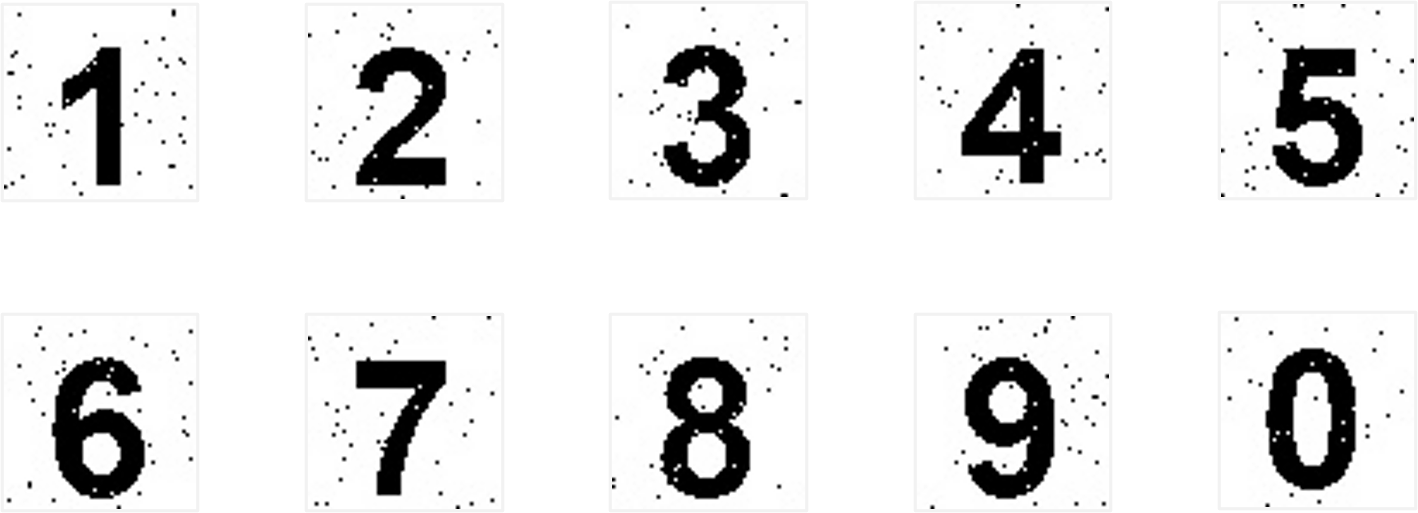
\includegraphics[width=.4\textwidth]{figuras/digitos_input.png}
    \caption{Exemplos de imagens $X$ a serem processadas com os dígitos $0-9$ e ruído sal e pimenta.}
    \label{fig:dig_X}
\end{figure}

\begin{figure}
    \centering
    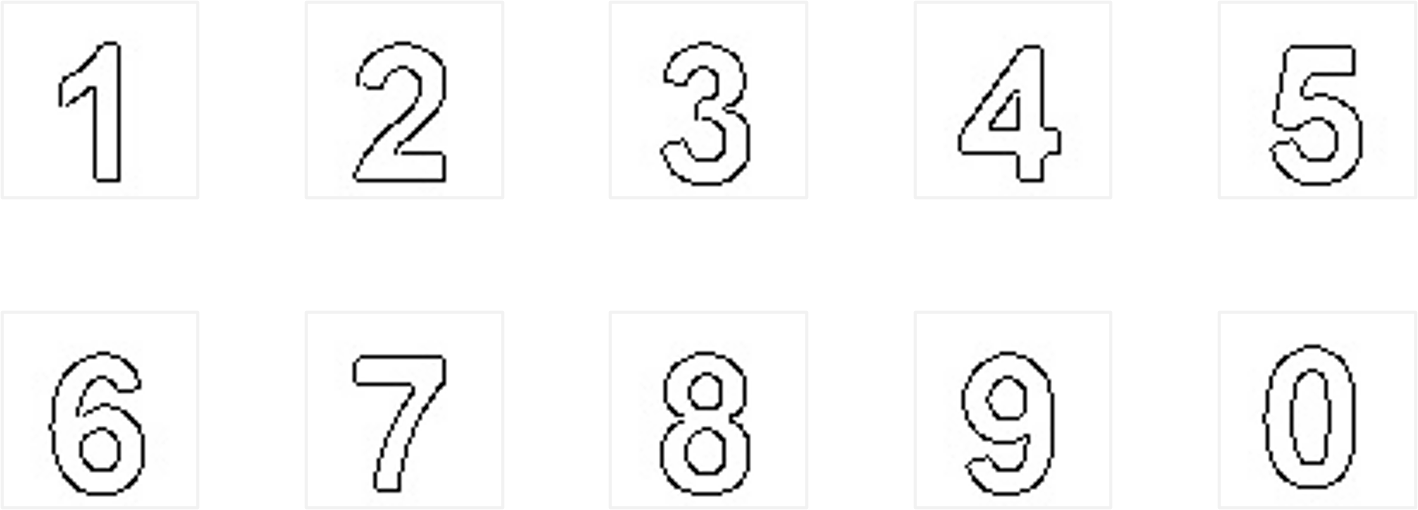
\includegraphics[width=.4\textwidth]{figuras/digitos_target.png}
    \caption{Exemplos de imagens $Y$ ideais com as bordas dos dígitos $0-9$ sem ruído.}
    \label{fig:dig_Y}
\end{figure}

Foram testadas diversas combinações de parâmetros para avaliar o desempenho do modelo, com a minimização do erro IoU, utilizando uma arquitetura de duas camadas ($n = 2$) e janelas 3x3 ($d_{W} = 3$). Os experimentos consideraram amostras de treinamento de 10 ou 30 imagens ($N = 10 \text{ ou } 30$) e amostras de validação de 10 imagens ($M = 10$). Para o reticulado das funções característica, foram amostrados 8 ou 16 vizinhos ($r = 8 \text{ ou } 16$), e para o reticulado da janela, 5 ou 9 vizinhos ($s = 5 \text{ ou } 9$). O processo de aprendizado da função característica foi conduzido por 100 épocas ($Epoch_f = 100$), enquanto o aprendizado da janela ocorreu por 50 épocas ($Epoch_w = 50$).

O tamanho do batch (batch size) variou de acordo com a quantidade de amostras de treinamento: batch de 5 ou 10 quando $N = 10$, e batch de 15 ou 30 quando $N = 30$. Para o critério de early stopping, foram utilizadas 30 épocas para o reticulado da função ($es_{f} = 30$) e 20 épocas para o reticulado da janela ($es_{w} = 20$). As janelas iniciais foram configuradas com uma estrutura em cruz ou com apenas o ponto central ativado ($W_{ini} = [[0,1,0],[1,1,1],[0,1,0]] \text{ ou } W_{ini} = [[0,0,0],[0,1,0],[0,0,0]]$). Todas essas configurações foram testadas de forma exaustiva, com variações feitas no esquema "todas contra todas", em que apenas um dos parâmetros era alterado por vez, mantendo os demais constantes.

Adicionalmente, foram realizados experimentos com uma única camada ($n = 1$), utilizando janelas 3x3 e 5x5 ($d_{W} = 3 \text{ ou } 5$), configuradas com os valores máximos para tamanho da amostra de treinamento, número de vizinhos amostrados, batch size e a janela inicial em cruz ($N = 30, r = 16, s = 9, b = 30, W_{ini} = [[0,1,0],[1,1,1],[0,1,0]]$), mantendo os demais parâmetros idênticos aos experimentos anteriores. Optou-se por não explorar extensivamente as combinações de parâmetros para uma única camada, dado que, devido à complexidade da solução, já se previa um desempenho inferior em comparação com as soluções de duas camadas. Esses experimentos serviram principalmente para evidenciar essa hipótese inicial.

Cada configuração de hiperparâmetros foi executada em uma \textit{run}, e cada \textit{run} foi repetida 10 vezes, alterando o parâmetro \textit{seed}. A \textit{seed} é um valor inicial que define a sequência de números produzidos pelo gerador de números aleatórios. Manter a mesma \textit{seed} e os mesmos parâmetros garante que, apesar da aleatoriedade inerente, os resultados sejam reprodutíveis. Portanto, considerar várias \textit{runs} com diferentes \textit{seeds} fornece uma visão mais robusta e confiável do desempenho do algoritmo sob diferentes condições de aleatoriedade.

Na Tabela \ref{tab:resultados_runs_digitos}, apresentamos os 10 melhores resultados das diferentes \textit{runs} ($R$). A tabela inclui os erros de treinamento ($L_{t}$), validação ($L_{v}$) e teste ($L_{tt}$) utilizando a notação "Valor Mínimo - Valor Médio (Desvio Padrão)". Ao final de cada execução calculou-se o erro de teste para cada uma das 10 \textit{seeds}, onde chegamos então no valor de erro de teste mínimo, médio e desvio padrão. Esse cálculo não teve interferência alguma nos treinamentos executados. Na tabela também temos a mínima época ($Epoch_{W_{min}}$ - época que obteve o menor erro de validação), os tempos em minutos de execução total de cada \textit{run} ($t_{total}$),  e o tempo para a mínima época ($t_{Epoch_{min}}$), estes também com a notação "Valor Mínimo - Valor Médio (Desvio Padrão)". Esses resultados fornecem uma visão abrangente do desempenho do algoritmo sob diferentes configurações de hiperparâmetros e \textit{seeds}. O critério de seleção das 10 melhores execuções foi: selecionar os 10 menores erros médios de teste e ordena-los pelo tempo de execução médio total. 

Na Tabela \ref{tab:hiperparametros_run} temos as configurações dos hiperparâmetros para cada uma das \textit{runs} selecionadas. A coluna $R$ indica cada \textit{run} da execução; $n$ é o número de camadas; $d_{W}$ é o tamanho da janela, $N$ e $M$ os tamanhos das amostras de treinamento e validação, respectivamente; $r$ e $s$ o número de vizinhos sorteados nos reticulados das funções característica e da janela, respectivamente; $Epoch_f$ e $Epoch_w$ as quantidade de épocas nos reticulados das funções característica e da janela, respectivamente; $b$ o tamanho do \textit{batch}; $es_f$ e $es_w$ os parâmetros de \textit{early stop} nos reticulados das funções característica e da janela, respectivamente; por fim, $W_{ini}$ é a configuração inicial dos W-operadores. 

No Apêndice \ref{apsec:reslts_digits} encontramos as tabelas \ref{tab:ap_resultados_runs_digitos} e \ref{tab:ap_hiperparametros_run} com os resultados completos de todas as execuções para esse experimento.

\begin{table}[ht]
    \centering
    \resizebox{\textwidth}{!}{ % Redimensiona a tabela para caber na largura da página
        \begin{tabular}{ccccccc}
            \toprule
            $R$ & $L_{t}$ & $L_{v}$ & $L_{tt}$ & $Epoch_{W_{min}}$ & $t_{total} \ (min)$ & $t_{Epoch_{min}} \ (min)$ \\
            \midrule
            17 & 0.0185 - 0.0757 (0.1405) & 0.0224 - 0.0775 (0.1397) & 0.0121 - 0.0167 (0.0023) & 13 - 29 (10) & 8.69 - 12.73 (1.91) & 2.63 - 7.45 (3.15) \\
            31 & 0.0195 - 0.0716 (0.1394) & 0.0227 - 0.0740 (0.1385) & 0.0128 - 0.0161 (0.0015) & 13 - 21 (7) & 9.60 - 13.53 (2.63) & 2.94 - 6.32 (2.54) \\
            16 & 0.0205 - 0.0371 (0.0297) & 0.0216 - 0.0384 (0.0292) & 0.0125 - 0.0152 (0.0017) & 12 - 30 (10) & 10.25 - 13.79 (1.53) & 3.51 - 8.64 (2.95) \\
            22 & 0.0209 - 0.0378 (0.0377) & 0.0217 - 0.0388 (0.0372) & 0.0124 - 0.0170 (0.0037) & 14 - 27 (11) & 11.06 - 15.26 (2.24) & 4.51 - 9.38 (3.95) \\
            25 & 0.0177 - 0.0708 (0.1398) & 0.0209 - 0.0729 (0.1389) & 0.0101 - 0.0156 (0.0030) & 20 - 33 (10) & 14.23 - 16.91 (1.49) & 5.32 - 11.00 (4.19) \\
            24 & 0.0173 - 0.0352 (0.0314) & 0.0203 - 0.0373 (0.0307) & 0.0110 - 0.0158 (0.0030) & 12 - 34 (12) & 14.09 - 18.55 (2.22) & 4.82 - 12.92 (4.59) \\
            20 & 0.0202 - 0.0333 (0.0300) & 0.0214 - 0.0346 (0.0295) & 0.0134 - 0.0156 (0.0015) & 8 - 25 (10) & 12.66 - 20.93 (3.30) & 3.23 - 11.90 (4.69) \\
            21 & 0.0183 - 0.0678 (0.1379) & 0.0208 - 0.0691 (0.1372) & 0.0123 - 0.0151 (0.0022) & 20 - 36 (9) & 19.90 - 21.84 (1.34) & 8.05 - 15.72 (4.50) \\
            29 & 0.0181 - 0.0674 (0.1405) & 0.0196 - 0.0697 (0.1395) & 0.0123 - 0.0145 (0.0018) & 14 - 37 (12) & 15.96 - 26.21 (4.55) & 4.80 - 19.49 (7.77) \\
            28 & 0.0171 - 0.0309 (0.0302) & 0.0198 - 0.0332 (0.0296) & 0.0104 - 0.0146 (0.0017) & 15 - 29 (10) & 19.92 - 27.70 (3.77) & 8.95 - 17.16 (6.07) \\

            \bottomrule
        \end{tabular}
    }
    \caption[Melhores 10 Runs experimentos dígitos]{Melhores 10 \textit{Runs}, cada uma com 10 execuções com \textit{seeds} diferentes. Erros IoU de treino, validação e teste, época que atingiu o menor erro de validação, tempos total e para atingir o menor erro de validação, calculados sob essas 10 execuções. Formato: Valor mínimo - Valor médio - Desvio padrão.}   
   % {Melhores 10 \textit{Runs}, cada uma com 10 execuções com \textit{seeds} diferentes. Erros IoU de treino, validação e teste, época que atingiu o menor erro de validação, tempos total e para atingir o menor erro de validação, calculados sob essas 10 execuções, no formato "Valor mínimo -- Valor médio (desvio padrão)".}
    \label{tab:resultados_runs_digitos}
\end{table}

\begin{table}[ht]
    \centering
    %\resizebox{\textwidth}{!}{ % Redimensiona a tabela para caber na largura da página
        \begin{tabular}{ccccccccccccc}
            \toprule
            $R$ & $n$ & $d_{w}$ & $N$ & $M$ & $r$ & $s$ & $Epoch_f$ & $Epoch_w$ & $b$ & $es_{f}$ & $es_{w}$ & $W_{ini}$ \\
            \midrule
            17 & 2 & 3 & 30 & 10 & 8 & 5 & 100 & 50 & 15 & 30 & 20 & Centro \\
            31 & 2 & 3 & 30 & 10 & 16 & 9 & 100 & 50 & 30 & 30 & 20 & Centro \\
            16 & 2 & 3 & 30 & 10 & 8 & 5 & 100 & 50 & 15 & 30 & 20 & Cruz \\
            22 & 2 & 3 & 30 & 10 & 8 & 9 & 100 & 50 & 30 & 30 & 20 & Cruz \\
            25 & 2 & 3 & 30 & 10 & 16 & 5 & 100 & 50 & 15 & 30 & 20 & Centro \\
            24 & 2 & 3 & 30 & 10 & 16 & 5 & 100 & 50 & 15 & 30 & 20 & Cruz \\
            20 & 2 & 3 & 30 & 10 & 8 & 9 & 100 & 50 & 15 & 30 & 20 & Cruz \\
            21 & 2 & 3 & 30 & 10 & 8 & 9 & 100 & 50 & 15 & 30 & 20 & Centro \\
            29 & 2 & 3 & 30 & 10 & 16 & 9 & 100 & 50 & 15 & 30 & 20 & Centro \\
            28 & 2 & 3 & 30 & 10 & 16 & 9 & 100 & 50 & 15 & 30 & 20 & Cruz \\
            \bottomrule
        \end{tabular}
   % }
    \caption[Configuração de hiperparâmetros das 10 melhores \textit{Runs} experimento dígitos]{Configuração de hiperparâmetros das 10 melhores \textit{Runs}: quantidade de camadas, tamanho da janela, tamanho da amostra de treinamento, tamanho da amostra de validação, quantidade de vizinhos do reticulado da função amostrados, quantidade de vizinhos no reticulado da janela amostrados, quantidade de épocas para o treinamento da função característica, quantidade de épocas para o treinamento da janela, tamanho do \textit{batch}, parâmetros de \textit{early stop} para os aprendizados da função e da janela, respectivamente e janela inicial de treinamento.}
    \label{tab:hiperparametros_run}
\end{table}

A análise das Tabelas \ref{tab:resultados_runs_digitos} e \ref{tab:hiperparametros_run}, que apresentam os resultados das 10 melhores execuções, demonstra de forma clara como a variação de diferentes hiperparâmetros influencia os erros e os tempos de execução. Observa-se que o aumento no tamanho da base de dados de treinamento ($N$) tende a favorecer uma melhor generalização do modelo. Este fato é evidenciado pelo fato de que todas as 10 melhores execuções utilizam o maior tamanho de amostra de treinamento testado (30 imagens). Além disso, o tamanho do \textit{batch} também mostrou ter uma influência significativa nos menores erros obtidos, com $80\%$ das execuções apresentando um \textit{batch} de tamanho $b=15$. \textit{Batches} menores permitem que o algoritmo percorra mais pontos do reticulado por época, o que contribui para uma busca mais eficaz pelo mínimo erro, além de escapar de regiões com alto erro. Por fim, a configuração com duas camadas de W-operadores 3x3 se destacou como a mais eficaz para esta solução, sendo consistentemente a escolhida em todas as 10 melhores execuções. Isso sugere que essa arquitetura de W-operadores multicamadas oferece um equilíbrio adequado entre complexidade e capacidade de captura de padrões relevantes, contribuindo de maneira decisiva para a obtenção dos melhores resultados.

Demais variações de hiperparâmetros, mantendo as configurações acima constantes, não produziram um impacto significativo no erro, mas afetaram consideravelmente o tempo de execução. Como esperado, o aumento no número de vizinhos sorteados nos reticulados tende a reduzir o erro, porém, à custa de um aumento substancial no tempo de execução. Por exemplo, ao comparar as execuções 17 e 28, observa-se que o erro médio de teste diminuiu de 0.0167 para 0.0146, representando uma redução de aproximadamente 12.6\%. Contudo, o tempo médio de execução aumentou de 12.73 minutos para 27.70 minutos, uma elevação de cerca de 117.6\%. Esse trade-off evidencia a necessidade de balancear a busca por menores erros com a eficiência computacional do algoritmo.

A Figura \ref{fig:validation_errors} apresenta os gráficos dos erros de validação ao longo das épocas do reticulado da janela para as seis execuções com menor erro médio. Cada subfigura representa uma execução específica corresponde aos parâmetros e resultados indicados nas tabelas \ref{tab:resultados_runs_digitos} e \ref{tab:hiperparametros_run}. As variações entre os gráficos refletem o impacto que diferentes seeds podem ter sobre o processo de treinamento com o mesmo parâmetro, especialmente em termos de convergência e minimização do erro de validação. Essa análise é fundamental para garantir que o modelo não apenas alcance um bom desempenho médio, mas também seja estável e confiável quando submetido a condições iniciais diferentes durante a fase de treinamento.

Outro ponto relevante a ser observado nos gráficos é a diferença significativa no erro inicial entre as execuções em que a janela inicial é o "Centro" (\textit{Runs} 21, 29 e 25) e aquelas em que a janela inicial é a "Cruz" (\textit{Runs} 16, 20 e 28). Nas execuções iniciadas com a janela "Centro", o erro inicial é substancialmente maior, o que impacta diretamente a quantidade de épocas necessárias para atingir o erro mínimo. Por exemplo, comparando as \textit{Runs} 28 e 29, observa-se um aumento de 29 para 37 épocas até encontrar o erro mínimo, o que representa um incremento de aproximadamente 27,6\% no número de épocas. Apesar desse aumento no número de épocas, o tempo médio de execução diminui de 27,70 para 26,21 minutos, uma redução de cerca de 5,4\%. Este fenômeno sugere que, embora o número de épocas da janela seja um fator importante, o algoritmo ainda depende do caminho no reticulado percorrido. No ponto inicial de cruz existe uma probabilidade maior de buscarmos em janelas mais complexas, inclusive a janela completa, que por consequência possui uma função característica maior e pode levar mais tempo na busca no reticulado da função.

\begin{figure}[H]
  \centering
  
  \begin{subfigure}{0.45\textwidth}
    \centering
    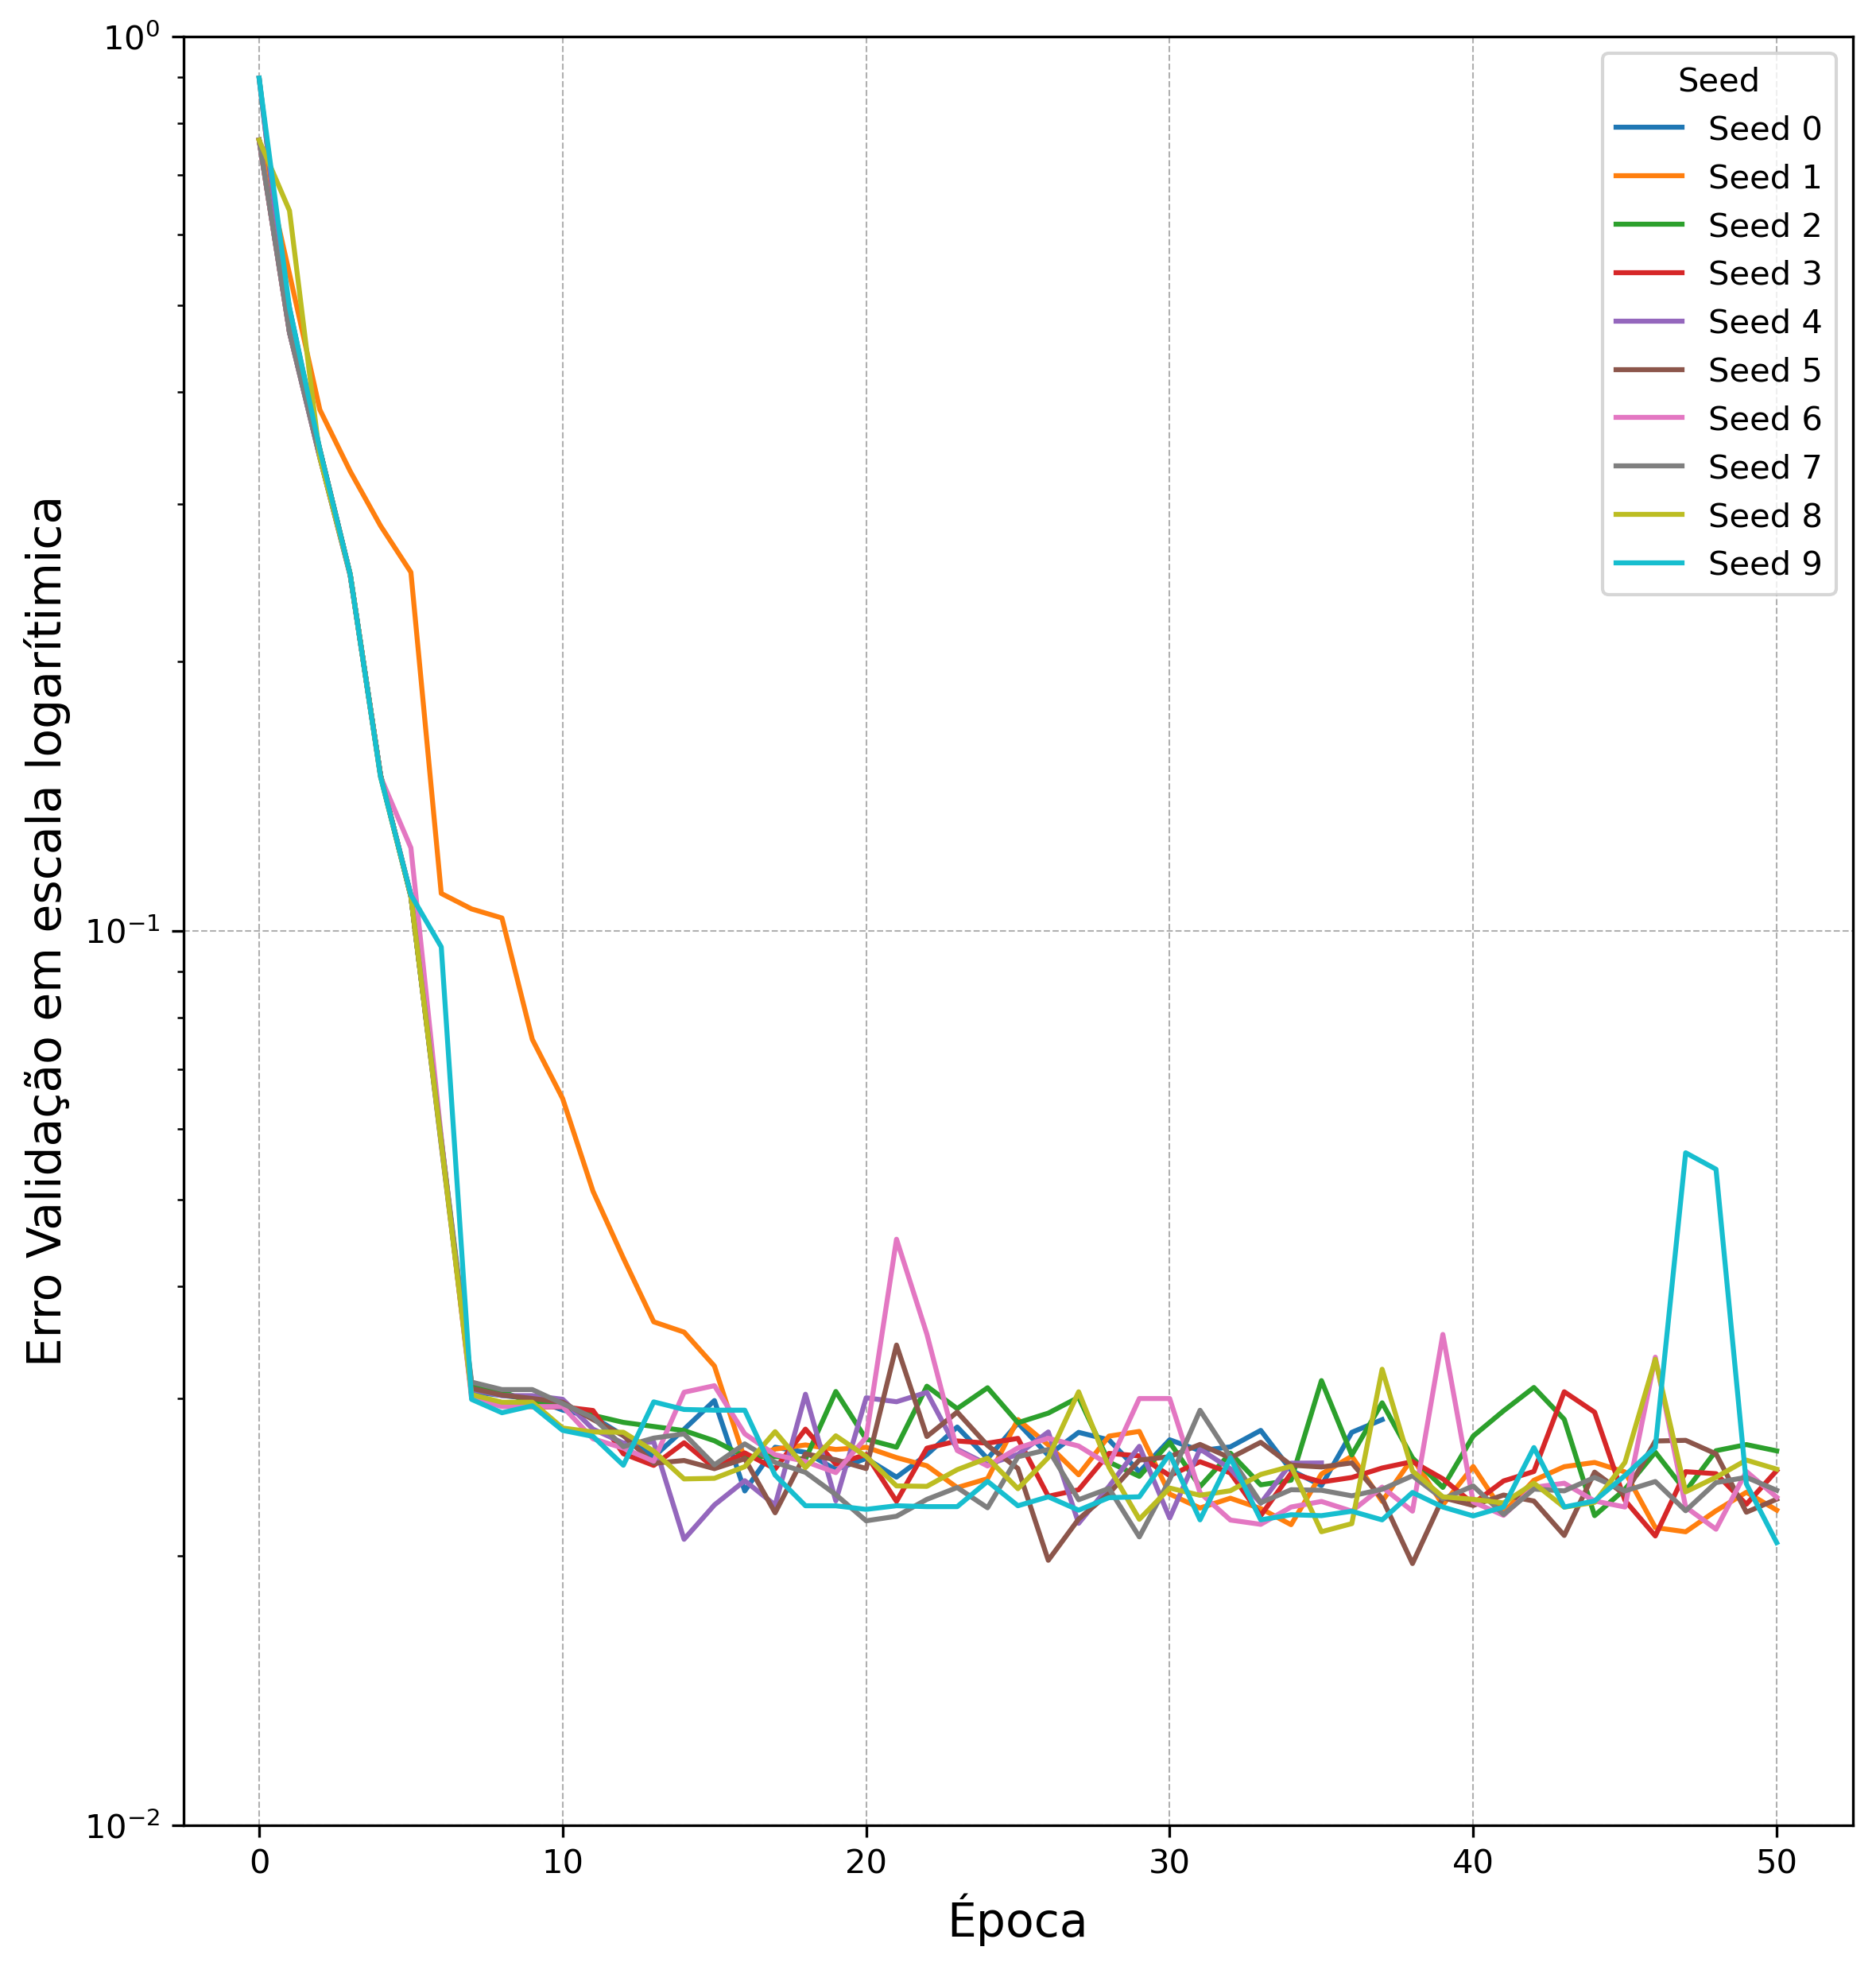
\includegraphics[width=\textwidth]{error_val_plot_29.png}
    \caption{Run 29 - $L_{tt_{mean}}=0.0145$}
  \end{subfigure}
  \hfill
  \begin{subfigure}{0.45\textwidth}
    \centering
    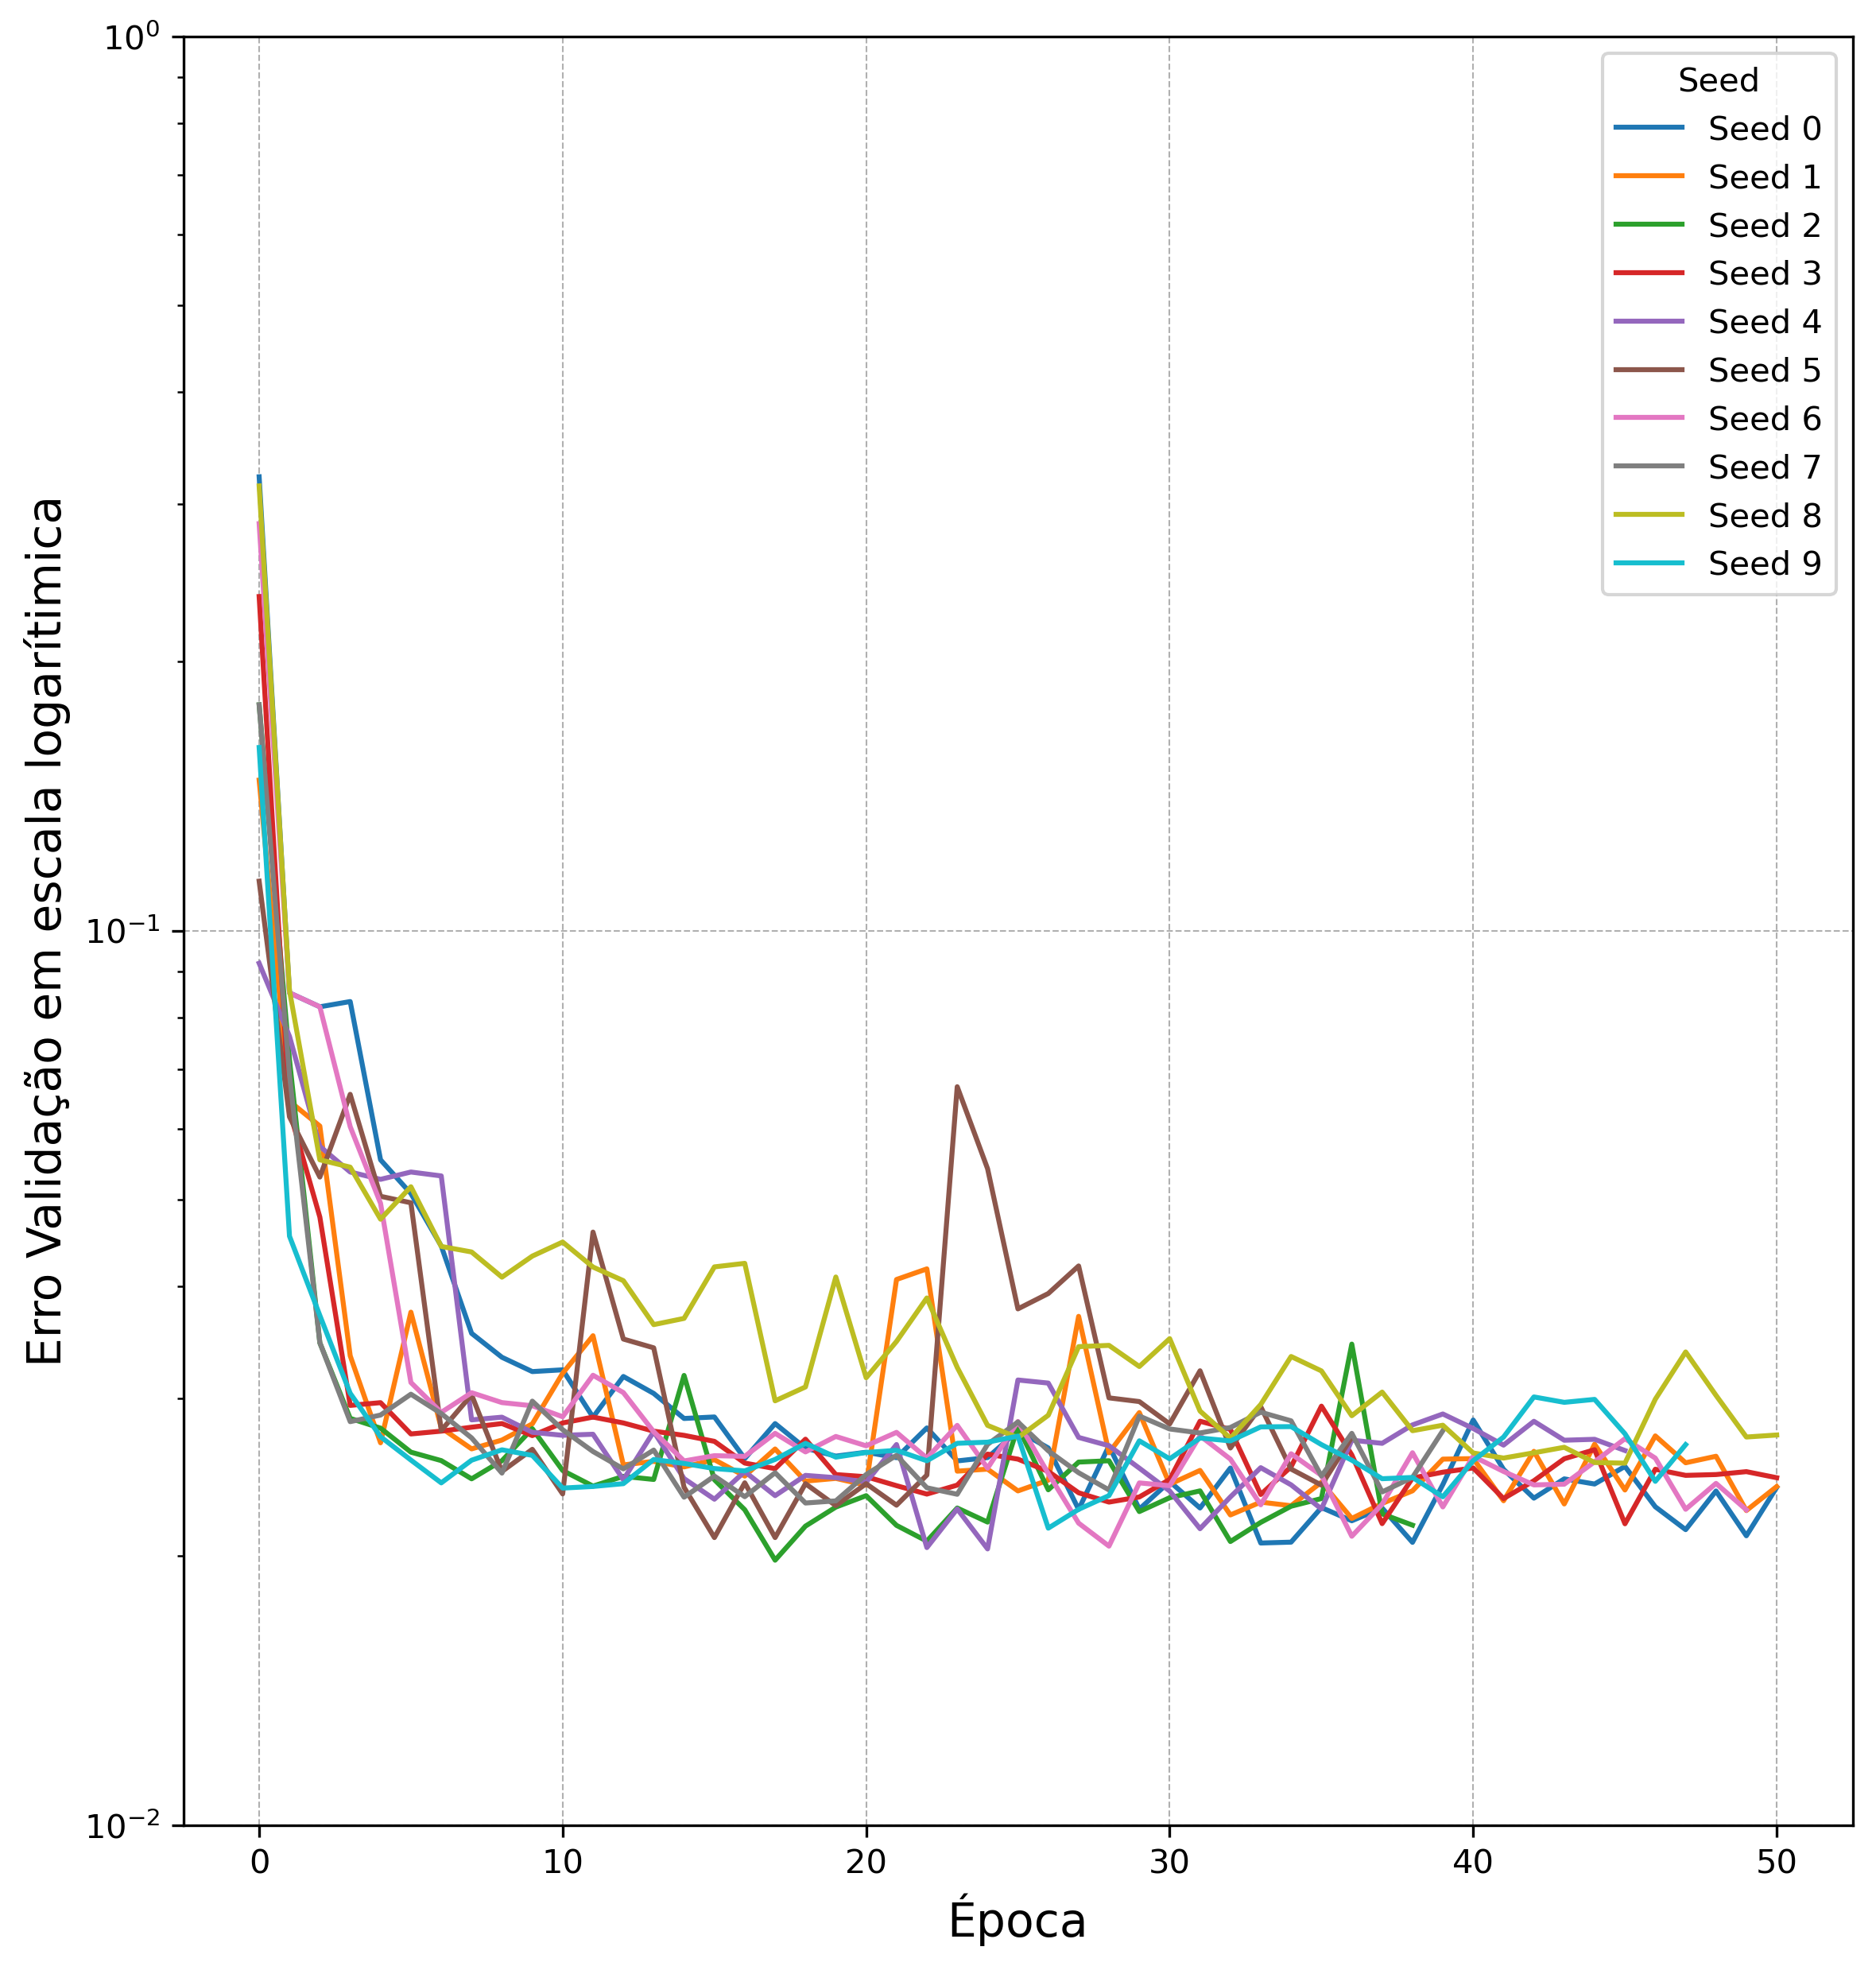
\includegraphics[width=\textwidth]{error_val_plot_28.png}
    \caption{Run 28 - $L_{tt_{mean}}=0.0146$}
  \end{subfigure}
  
  \vspace{0.3cm}
  
  \begin{subfigure}{0.45\textwidth}
    \centering
    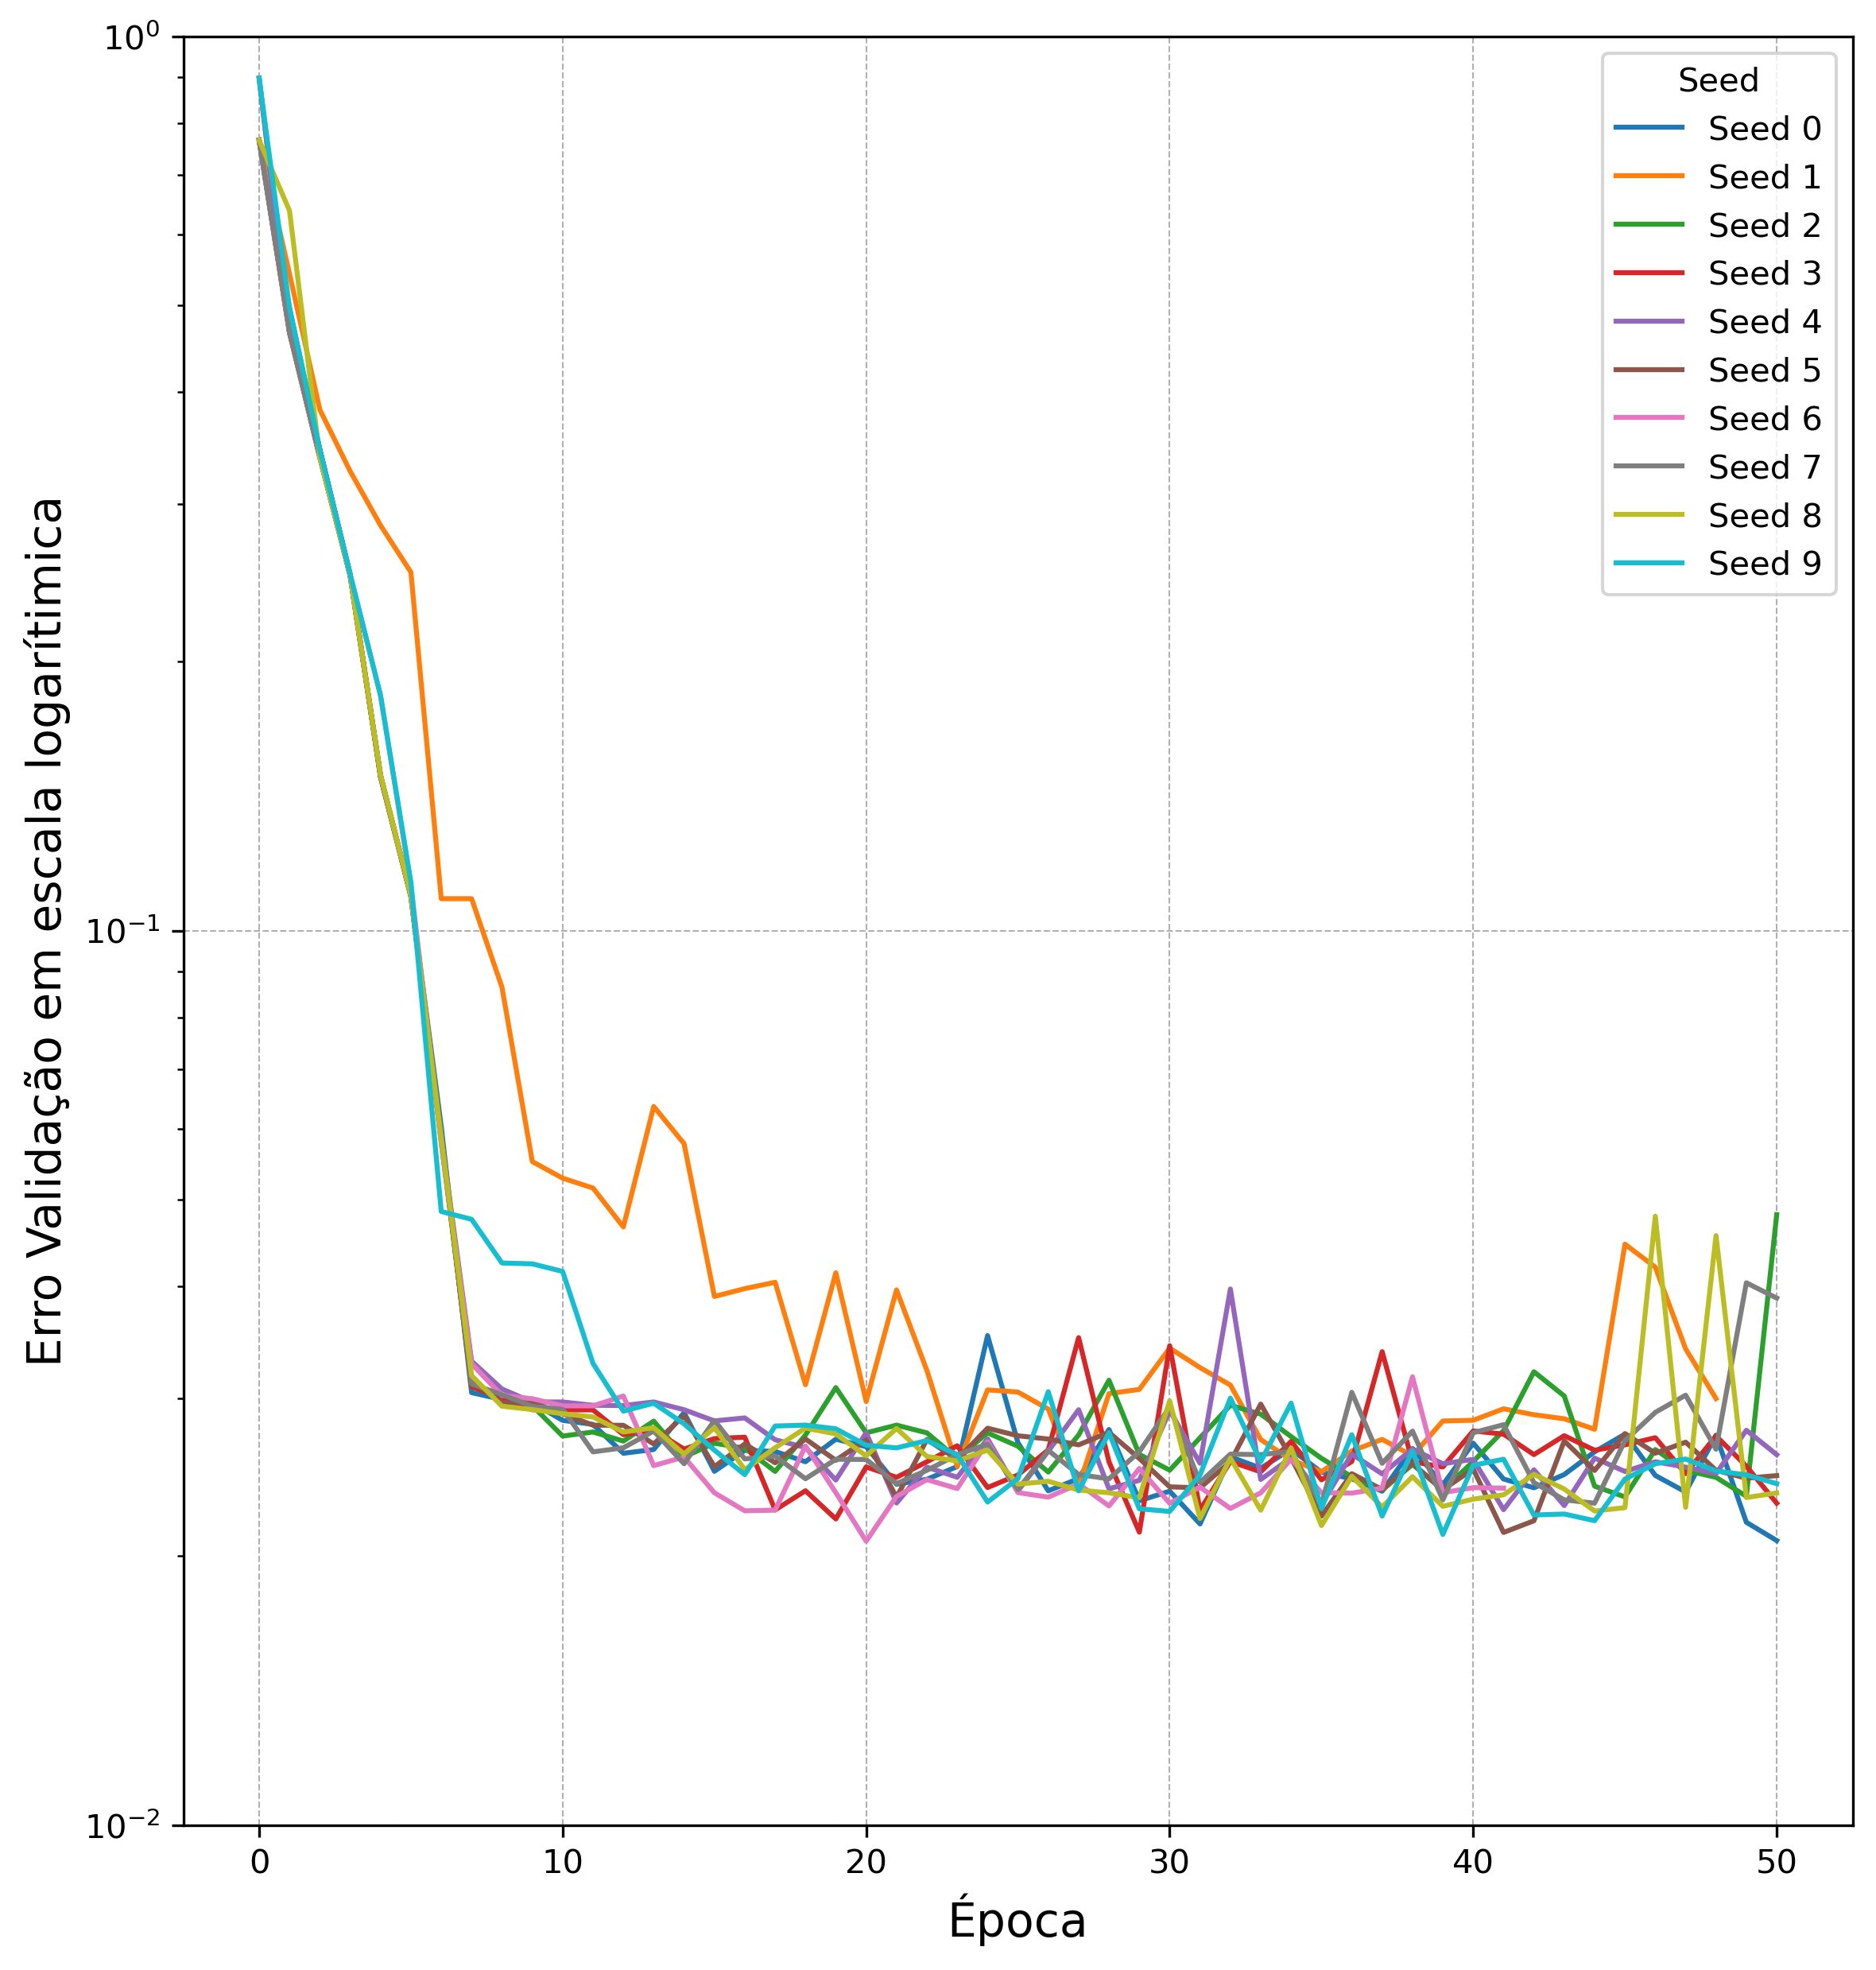
\includegraphics[width=\textwidth]{error_val_plot_21.png}
    \caption{Run 21 - $L_{tt_{mean}}=0.0151$}
  \end{subfigure}
  \hfill
  \begin{subfigure}{0.45\textwidth}
    \centering
    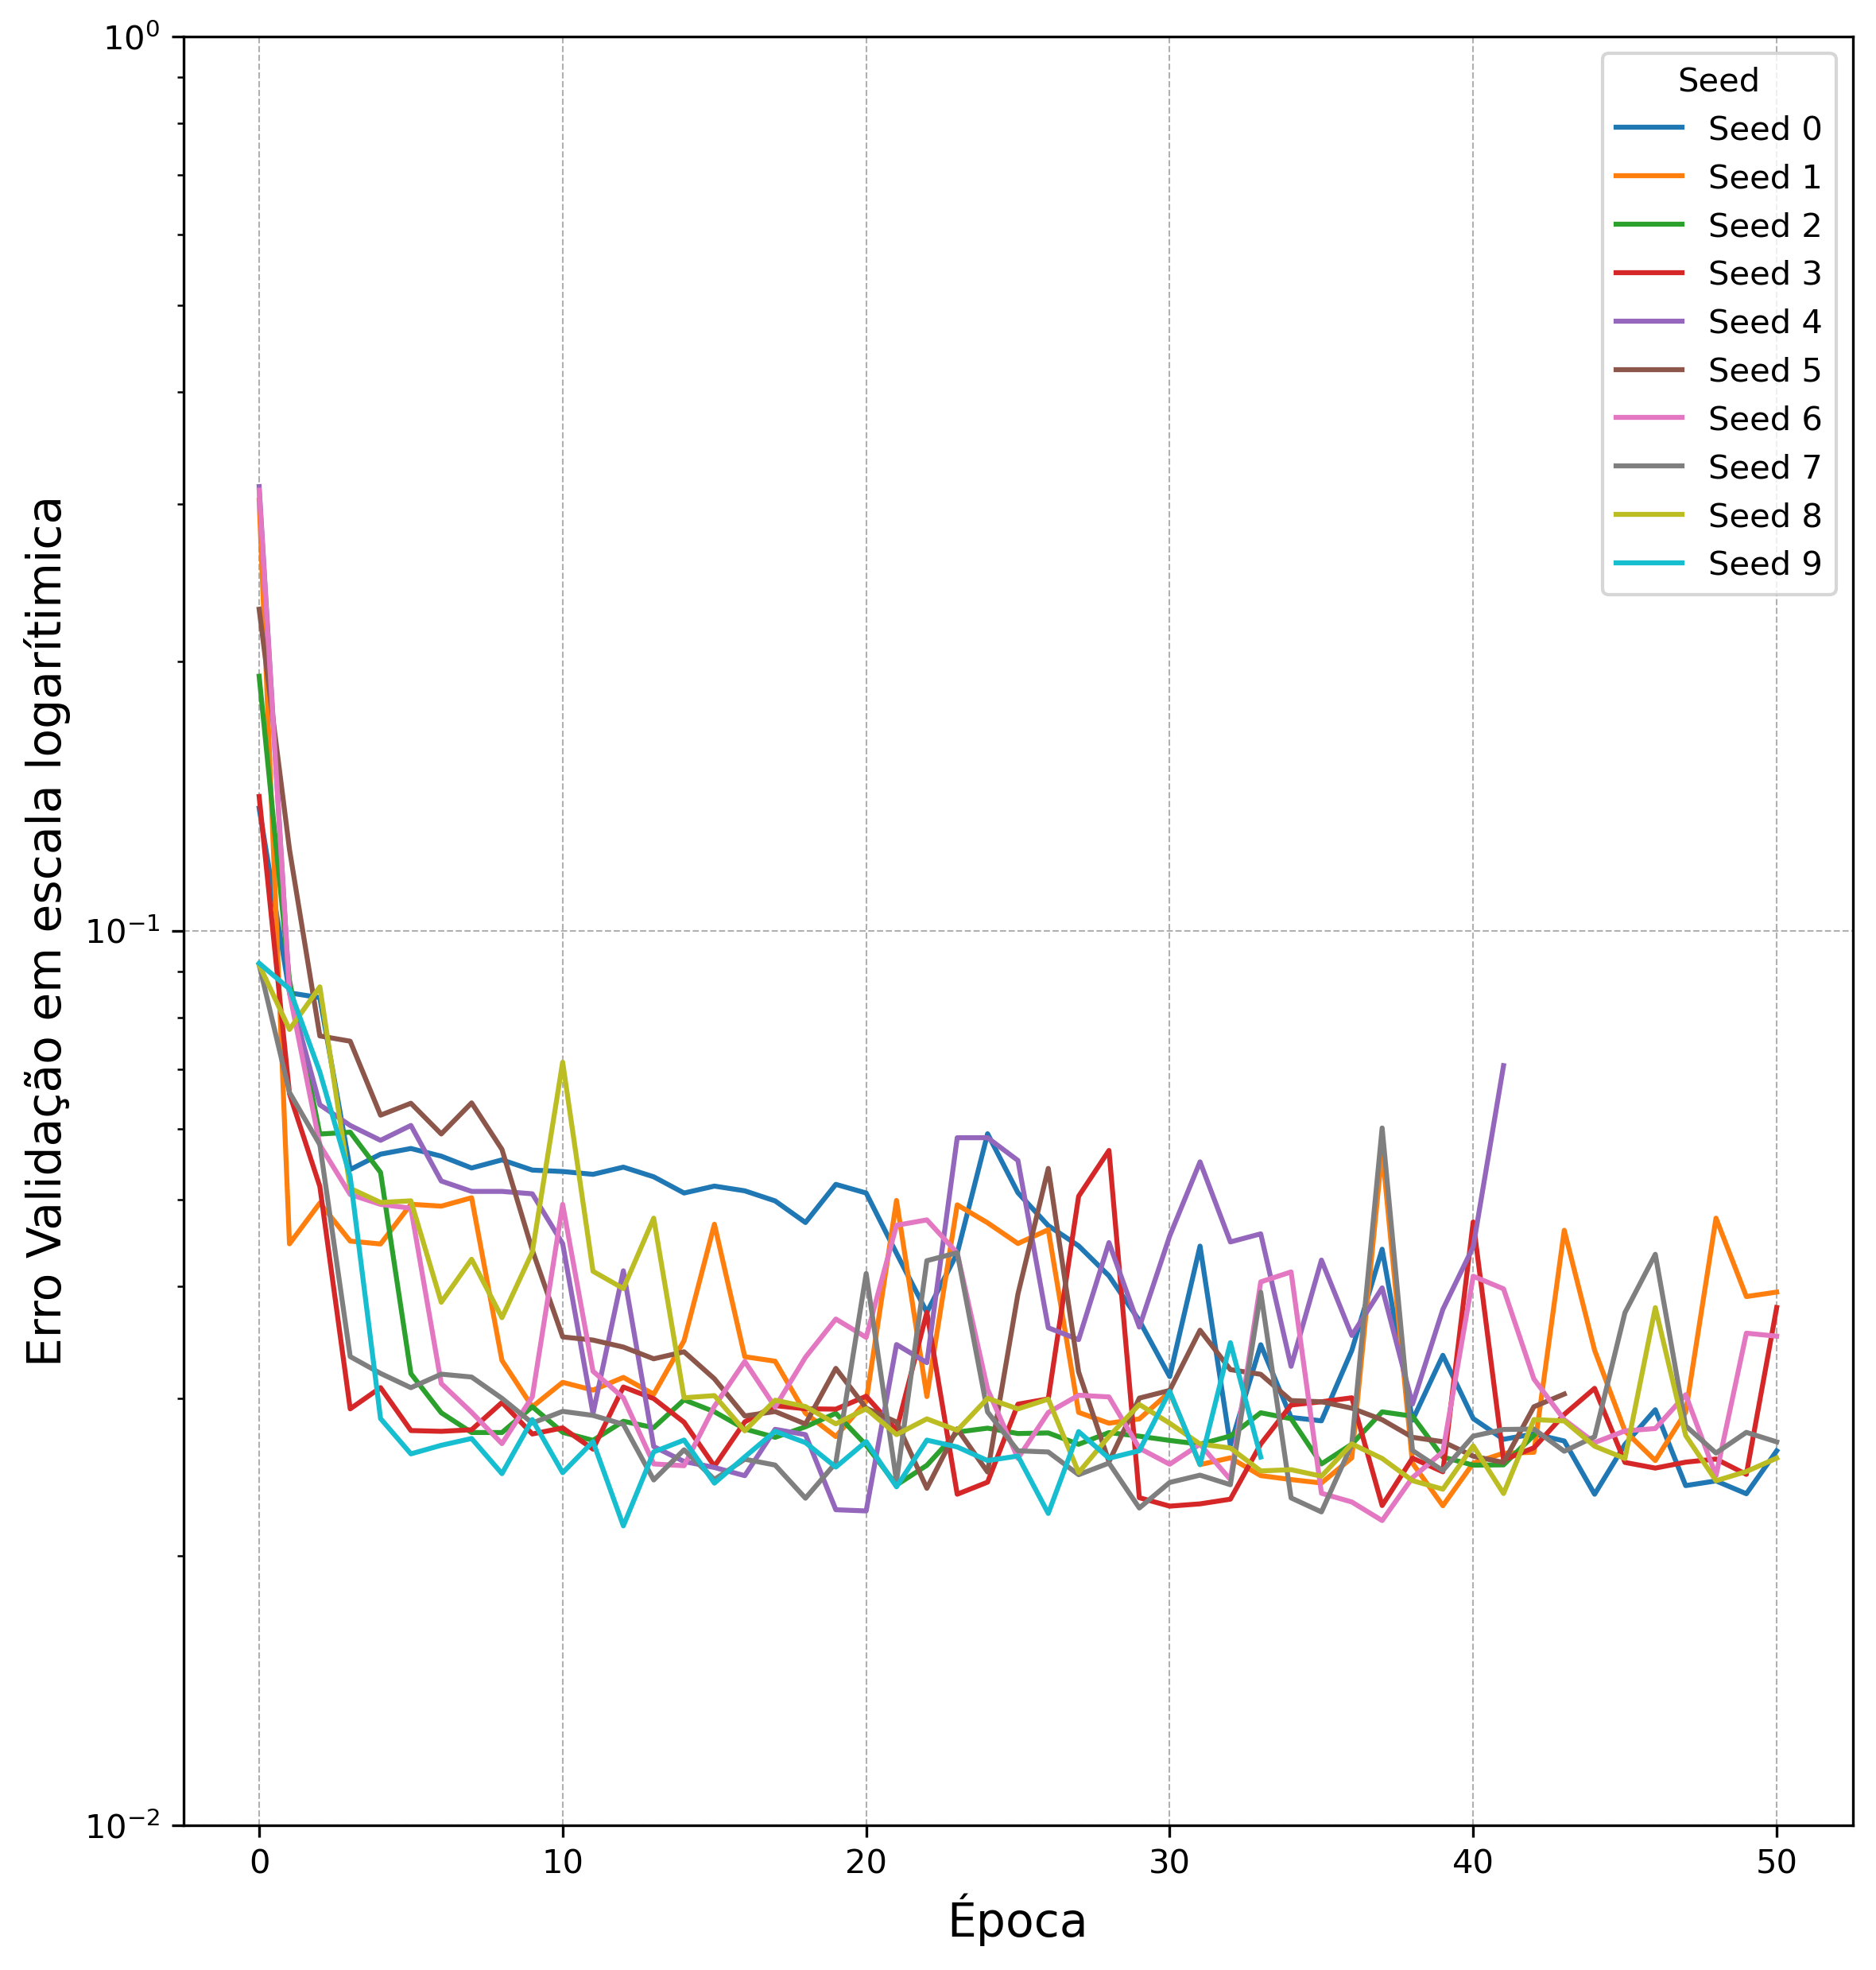
\includegraphics[width=\textwidth]{error_val_plot_16.png}
    \caption{Run 16 - $L_{tt_{mean}}=0.0152$}
  \end{subfigure}
  
  \vspace{0.3cm}
  
  \begin{subfigure}{0.45\textwidth}
    \centering
    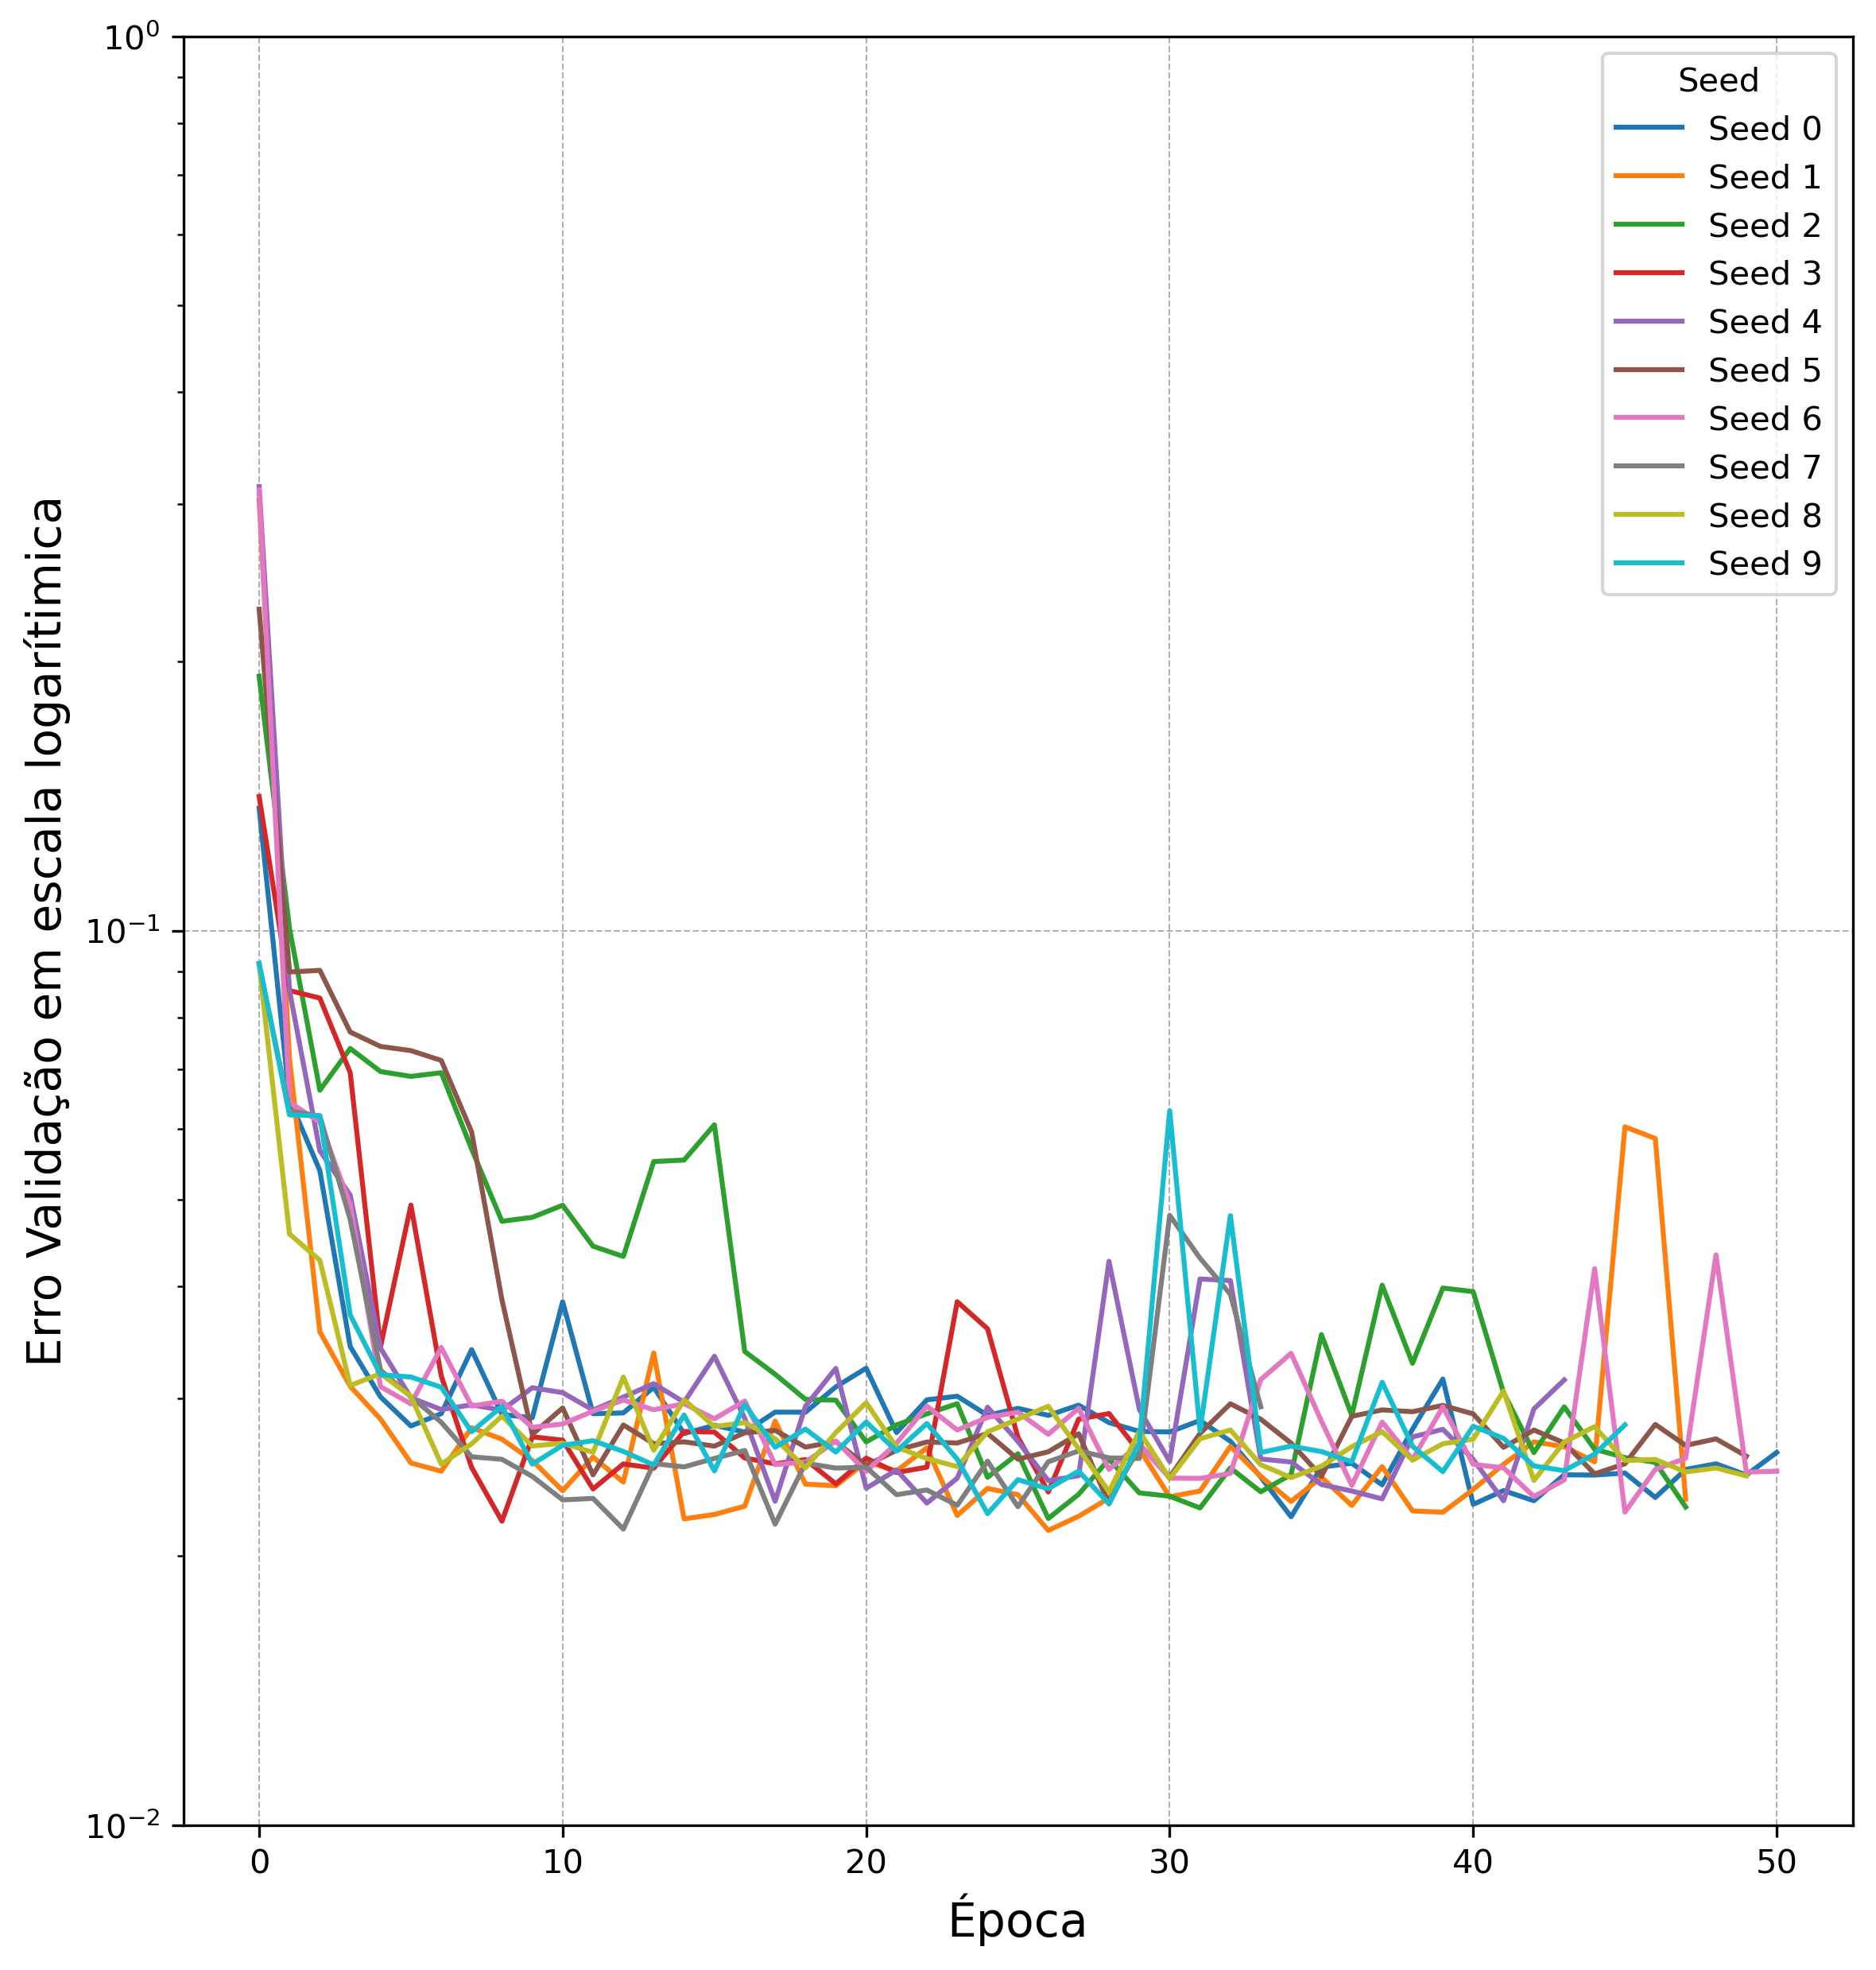
\includegraphics[width=\textwidth]{error_val_plot_20.png}
    \caption{Run 20 - $L_{tt_{mean}}=0.0156$}
  \end{subfigure}
  \hfill
  \begin{subfigure}{0.45\textwidth}
    \centering
    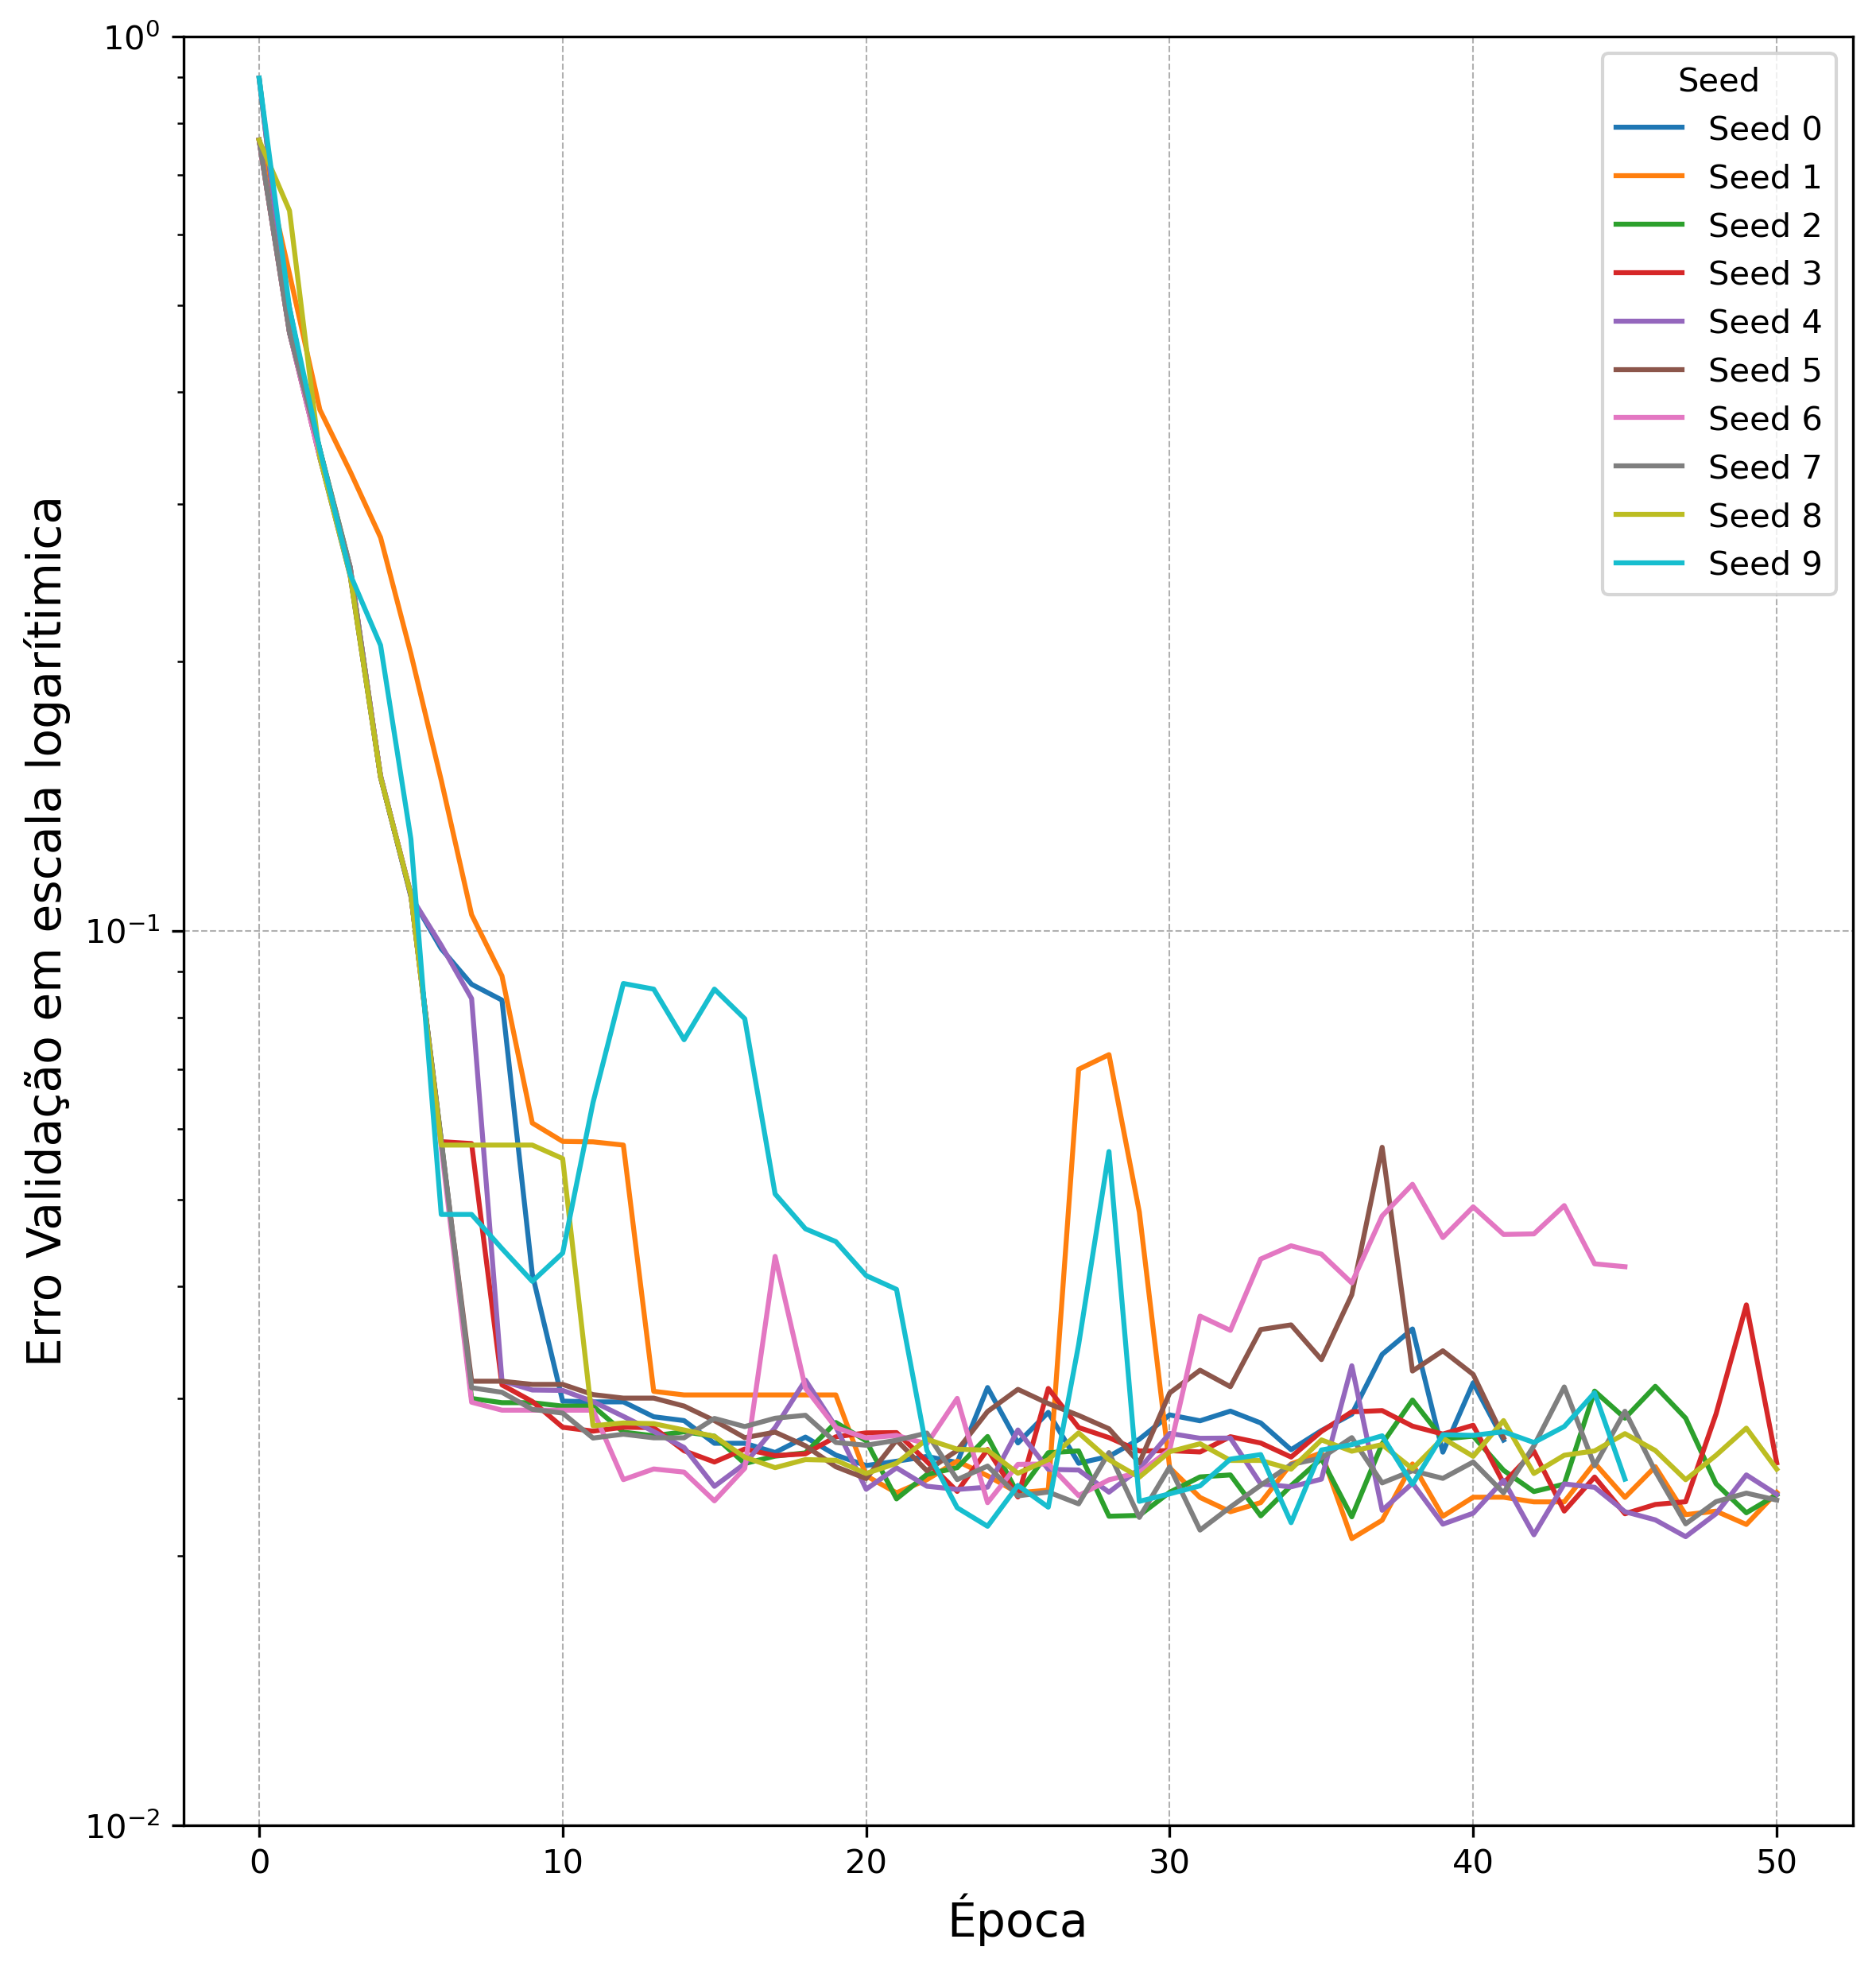
\includegraphics[width=\textwidth]{error_val_plot_25.png}
    \caption{Run 25 - $L_{tt_{mean}}=0.0156$}
  \end{subfigure}

  \caption{Erros de validação ao longo das épocas para as 6 execuções com menor erro médio usando diferentes seeds.\label{fig:validation_errors}}
\end{figure}


Entre todas as execuções, a \textit{Run} 21 - \textit{seed} 1 apresentou o menor erro, com os seguintes resultados: erro de treinamento $L_{t} = 0.0177$, erro de validação $L_{v} = 0.0209$ e erro de teste $L_{tt} = 0.0101$. O tempo total de execução foi de 16.80 minutos, sendo que o erro mínimo foi alcançado na época 36, após 11.25 minutos de processamento. 

Em \cite{DIEGO:DMM}, diversas arquiteturas de redes morfológicas discretas (CDMNN) foram avaliadas com o mesmo conjunto de dados deste experimento, destacando-se a arquitetura \texttt{asf3\_8sg3\_8sg3} com \textit{batch} 5, que apresentou os melhores resultados. Os erros reportados foram de treino $L_{t} = 0.036 - 0.068 \ (0.028)$ e de validação $L_{v} = 0.046 - 0.081 \ (0.025)$, ambos expressos no formato "Valor Mínimo - Valor Médio (Desvio Padrão)". Diferentemente do algoritmo proposto neste trabalho, as CDMNN não utilizam o erro de validação durante o treinamento, sendo o erro de validação equiparado ao erro de teste para fins de comparação. Observa-se que todos os resultados apresentados na Tabela \ref{tab:resultados_runs_digitos} superam o melhor resultado obtido em \cite{DIEGO:DMM}. Em particular, o menor erro de teste obtido, $L_{tt} = 0.0101$, na \textit{Run} 25, é 78\% inferior ao valor mínimo de $0.046$ reportado por \cite{DIEGO:DMM}. Este resultado destaca a superioridade do nosso método para a aplicação em questão.

As imagens de saída após a aplicação em $X$ do primeiro W-operador aprendido nesta execução, são apresentadas na Figura \ref{fig:output_op1}, enquanto o resultado final, após a aplicação dos dois W-operadores, é exibido na Figura \ref{fig:output_op2}. 

Cada camada do W-operador especializou-se em uma tarefa distinta, mesmo sem a imposição de restrições específicas no algoritmo de aprendizado e sendo treinadas em conjunto. A primeira janela foi responsável pela filtragem do ruído sal e pimenta, enquanto a segunda janela realizou a extração das bordas. Esses resultados sugerem que W-operadores podem ter tendência a se especializar na realização de tarefas distintas de forma eficaz, mesmo quando treinados em conjunto, o que implica que camadas distintas em uma arquitetura multicamadas têm a capacidade de se especializar em diferentes tipos de tarefas. Essa observação indica um potencial a ser investigado nos W-operadores em arquiteturas multicamadas, pois cada camada pode se especializar em uma tarefa específica, o que pode levar a um desempenho mais robusto e eficiente. Um fator importante a se considerar é o papel da inicialização dos W-operadores, que pode direcionar o percurso pelos reticulados a diferentes regiões do espaço de soluções, favorecendo a especialização em tarefas distintas.

\begin{figure}
    \centering
    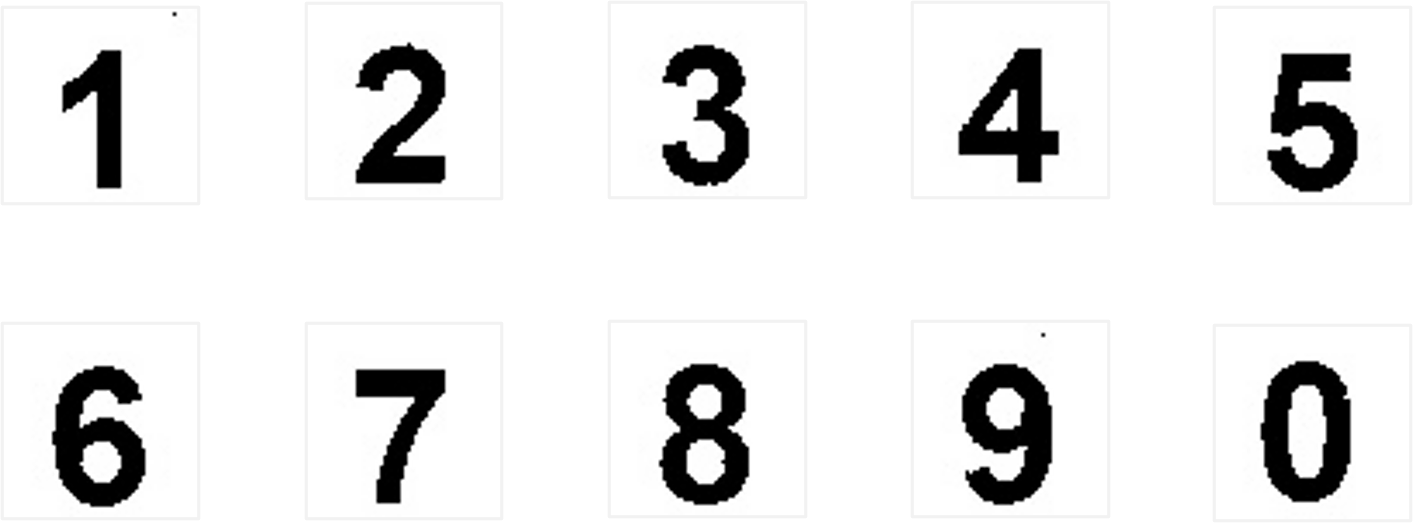
\includegraphics[width=.4\textwidth]{figuras/digitos_output_op1.png}
    \caption{Imagem de saída após aplicar apenas o primeiro W-operador aprendido.}
    \label{fig:output_op1}
\end{figure}


\begin{figure}
    \centering
    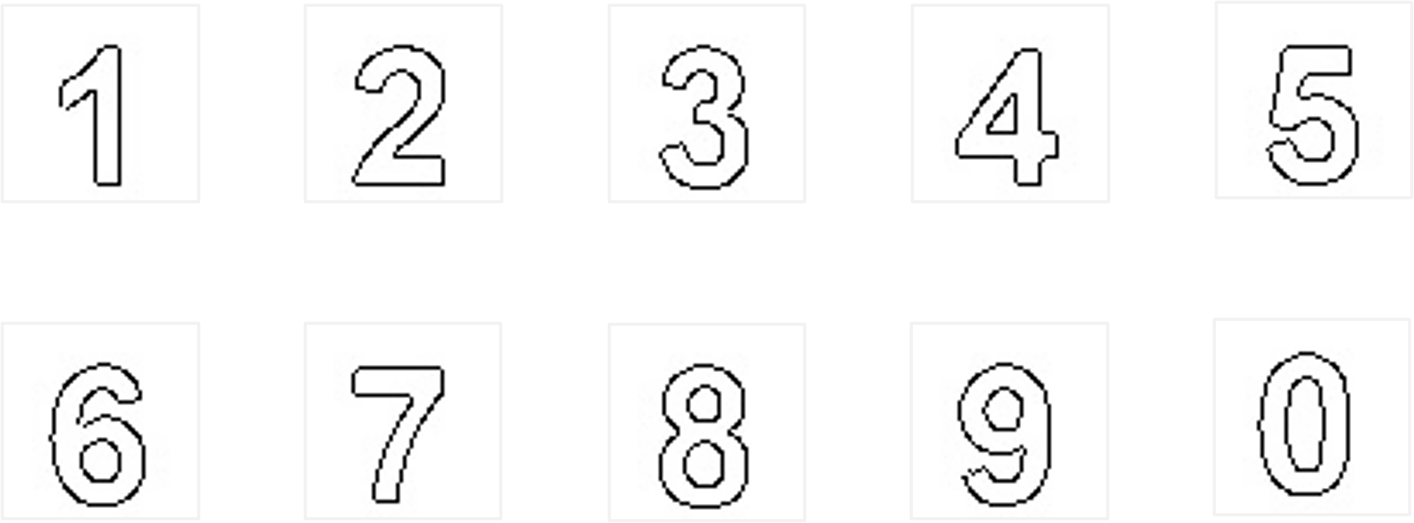
\includegraphics[width=.4\textwidth]{figuras/digitos_output_op2.png}
    \caption{Imagem final de saída após aplicar o WOMC completo aprendido.}
    \label{fig:output_op2}
\end{figure}

Os elementos estruturantes das janelas finais aprendidas pelo algoritmo podem ser observadas na Figura \ref{fig:WOMC}. Nas tabelas \ref{tab:func_w1} e \ref{tab:func_w2} do Apêndice \ref{apsec:reslts_digits} temos as função características completas aprendidas para as duas janelas.

\begin{figure}
  \centering

  \begin{subfigure}{0.4\textwidth}
    \centering
    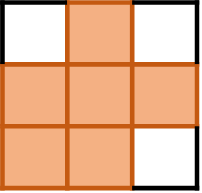
\includegraphics[width=.4\textwidth]{figuras/wop_1.png}
    \caption{Janela $W_{1}$\label{fig:subfig:w1}}
  \end{subfigure}
  \begin{subfigure}{0.4\textwidth}
    \centering
      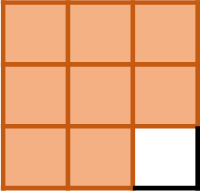
\includegraphics[width=.4\textwidth]{figuras/wop_2.png}
    \caption{Janela $W_{2}$\label{fig:subfig:w1}}
  \end{subfigure}

  \caption{Janelas do WOMC estimadas para realizar a filtragem do ruído sal e pimenta e extração das bordas dos dígitos $0-9$.\label{fig:WOMC}}
\end{figure}

Os resultados obtidos corroboram a afirmação da Introdução \ref{sec:motiv}, já que os resultados representados pelos W-operadores, diferentemente de diversos métodos modernos de aprendizado baseados em redes neurais, são \textbf{interpretáveis}, pois, através do elemento estruturante e funções características dos W-operadores finais de cada camada é possível deduzir matematicamente as propriedades de cada W-operador; e \textbf{possuem consistência lógica, transparência do método e uma boa performance}, uma vez que o erro IoU de 0.0101 é muito baixo, principalmente ao levar em conta que foi utilizada uma amostra de somente 40 imagens para o aprendizado (30 de treino e 10 de validação).

\section{Aprendizado do W-operador de transição do \textit{Conway's Game of Life}}
\label{sec:GoL}

O \textit{Conway's Game of Life} \cite{GOL}, que por simplificação chamaremos a partir de agora de \textbf{GoL}, criado por John Conway em 1970, é um autômato celular que simula a evolução de células em uma grade bidimensional de acordo com um conjunto de regras simples. Cada célula da grade pode estar em um de dois estados possíveis: viva $(1)$ ou morta $(0)$. A evolução do sistema ocorre em passos discretos de tempo, onde o estado de cada célula na próxima geração é determinado por suas células vizinhas, seguindo as seguintes regras:

\begin{itemize}
    \item \textbf{Sobrevivência}: Uma célula viva com dois ou três vizinhos vivos permanece viva na próxima geração.
    \item \textbf{Morte por solidão}: Uma célula viva com menos de dois vizinhos vivos morre, como se fosse por solidão.
    \item \textbf{Morte por superpopulação}: Uma célula viva com mais de três vizinhos vivos morre, devido à superpopulação.
    \item \textbf{Nascimento}: Uma célula morta com exatamente três vizinhos vivos se torna viva, representando o nascimento de uma nova célula.
\end{itemize}

Essas regras fazem com que padrões complexos e dinâmicos emerjam a partir de configurações iniciais simples, tornando o \textbf{GoL} um exemplo clássico de como comportamentos complexos podem surgir de regras simples.

No contexto do nosso experimento, o \textbf{GoL} pode ser visto como uma transformação de imagens, onde as regras do jogo correspondem a um W-operador 3x3 de uma camada, com todos os pontos da janela preenchidos. O W-operador, nesse caso, processa a imagem binária inicial (com células vivas e mortas) para gerar uma nova imagem (o estado seguinte do autômato) com base nas regras pré-definidas.

Esse experimento é particularmente interessante porque o \textbf{GoL} possui uma função de transição conhecida, que é definida precisamente pelas regras do jogo. Essa função está expressa por completo no apêndice \ref{apsec:reslts_gol}. Portanto, podemos avaliar a capacidade do modelo de aprender e replicar um sistema com uma solução exata.

Para aprender a função de transição do \textbf{GoL}, realizamos experimentos utilizando uma configuração com 1 camada ($n=1$) e janelas 3x3 ($d_{W} = 3$). Foram testadas diferentes quantidades de imagens de treinamento ($N = 100 \text{ ou } 300$) e de validação ($M = 100 \text{ ou } 300$) selecionadas aleatóriamente do dataset "GoL\_final", com 16 vizinhos amostrados tanto para a função ($r=16$) quanto para a janela ($s=16$). O aprendizado da função característica ocorreu ao longo de 2000 épocas ($Epoch_f = 2000$) e o aprendizado da janela ao longo de 200 épocas ($Epoch_w = 200$). Utilizou-se um tamanho de batch de 50 ($b=50$), com critério de early stopping para o reticulado da função após 50 épocas ($es_{f} = 50$) e para o reticulado da janela após 10 épocas ($es_{w} = 10$). A janela inicial foi configurada em cruz ($W_{ini} = [[0,1,0],[1,1,1],[0,1,0]]$).

O aprendizado foi realizado com o erro MAE, utilizando diferentes níveis de ruído nas imagens de saída, como segue:

\begin{enumerate}
    \item Imagens de saída originais.
    \item Imagens de saída com 5\% de ruído sal e pimenta.
    \item Imagens de saída com 10\% de ruído sal e pimenta.
    \item Imagens de saída com 15\% de ruído sal e pimenta.
    \item Imagens de saída com 20\% de ruído sal e pimenta.
    \item Imagens de saída com 30\% de ruído sal e pimenta.
\end{enumerate}

A descrição de como o dataset "GoL\_final" foi criado está descrita no apêndice \ref{apsec:reslts_gol}.

O objetivo de incluir o ruído sal e pimenta nas imagens de saída é avaliar se o algoritmo é robusto ao ruído e consegue identificar a função de transição, especialmente em cenários de maior dificuldade, como no caso de 30\% de ruído.

Além do aprendizado tradicional de Janela + Função Característica, foi realizado, para cada um dos cenários, um aprendizado apenas da função, fixando a janela ótima (quadrado 3x3). Nesse caso, não utilizamos a estocasticidade no sorteio dos vizinhos ($r$), realizando uma busca completa no reticulado, com o objetivo de encontrar a função ótima.

Após o término de cada treinamento, os resultados foram comparados com a função de transição já conhecida.

Na Tabela \ref{tab:resultados_gol} , apresentamos os resultados das \textit{Runs} ($R$) de 1 a 12, representando cada um dos experimentos, a coluna $Ruido$ indica o percentual de ruído nesse experimento e a coluna $N$ a quantidade de dados da amostra de treinamento. Em cada experimento tivemos 10 execuções com \textit{seeds} diferentes, ou seja, pontos iniciais diferentes. O cálculo de erro de validação ($L_{v}$) refere-se ao erro durante o processo de validação do aprendizado do algoritmo, apresentado na notação "Valor Mínimo - Valor Médio (Desvio Padrão)" \ calculado sobre as 10 diferentes \textit{seeds} de cada \textit{Run}.

Além disso, a tabela inclui a quantidade de execuções, dentre as 10, em que a função ótima foi aprendida ($P_{f_{ideal}}$) para o aprendizado do algoritmo completo e a quantidade de execuções em que a função ótima foi aprendida ($P_{f_{ideal}-fixed}$) para o aprendizado com janela fixa; Por fim, os percentuais de erro entre a função aprendida e a função de transição conhecida, também para os dois aprendizados sendo denotado por $error_{f_{ideal}}$ e $error_{f_{ideal}-fixed}$, os tempos de aprendizado do algoritmo completo ($t_{total}$) e do algoritmo com janela fixa ($t_{W_{fixed}}$), todos no formato "Valor Mínimo - Valor Médio (Desvio Padrão)".

\begin{table}[ht]
    \centering
    \resizebox{\textwidth}{!}{ % Redimensiona a tabela para caber na largura da página
        \begin{tabular}{ccccccccccc}
            \toprule
            $R$ & $Ruido$ & $N$ & $M$ & $L_{v}$ & $P_{f_{ideal}}$ & $error_{f_{ideal}}$ \ (\%) & $P_{f_{ideal}-fixed}$ & $error_{f_{ideal}-fixed}$ \ (\%) & $t_{total} \ (min)$ & $t_{W_{fixed}} \ (min)$  \\
            \midrule
            1 & 0\%  & 100 & 100 & $0.0015 - 0.0514 \ (0.0492)$ & $0$ & $1.56 - 2.45 \ (0.42)$ &$0$ & $0.20 - 0.39 \ (0.15)$ & $4.10 - 5.98 \ (1.40)$ & $6.55 - 7.26 \ (0.31)$ \\
            2 & 5\%  & 100 & 100 & $0.0681 - 0.1092 \ (0.0418)$ & $0$ & $2.34 - 2.82 \ (0.39)$ & $0$ & $0.20 - 0.39 \ (0.15)$ & $4.00 - 7.91 \ (2.20)$ & $6.61 - 7.03 \ (0.36)$ \\
            3 & 10\% & 100 & 100 & $0.1220 - 0.1617 \ (0.0397)$ & $0$ & $2.34 - 2.93 \ (0.43)$ & $0$ & $0.59 - 0.90 \ (0.20)$ & $3.90 - 7.21 \ (2.55)$ & $7.21 - 8.39 \ (0.67)$ \\
            4 & 15\% & 100 & 100 & $0.1807 - 0.2161 \ (0.0350)$ & $0$ & $2.15 - 3.17 \ (0.52)$ & $0$ & $0.39 - 0.67 \ (0.15)$ & $4.08 - 8.40 \ (2.48)$ & $11.12 - 14.27 \ (2.10)$ \\
            5 & 20\% & 100 & 100 & $0.2429 - 0.2746 \ (0.0319)$ & $0$ & $3.32 - 3.89 \ (0.48)$ & $0$ & $1.37 - 1.57 \ (0.20)$ & $4.28 - 7.07 \ (1.52)$ & $12.89 - 17.20 \ (2.04)$ \\
            6 & 30\% & 100 & 100 & $0.3643 - 0.3866 \ (0.0221)$ & $0$ & $4.49 - 5.49 \ (0.63)$ & $0$ & $8.01 - 9.50 \ (0.92)$ & $4.72 - 6.14 \ (1.05)$ & $11.96 - 23.66 \ (4.68)$ \\
            7 & 0\%  & 300 & 300 & $0.0014 - 0.0516 \ (0.0507)$ & $0$ & $1.76 - 2.25 \ (0.36)$ & $10$ & $0.00 - 0.00 \ (0.00)$ & $9.49 - 16.80 \ (7.81)$ & $3.10 - 3.29 \ (0.10)$ \\
            8 & 5\%  & 300 & 300 & $0.0641 - 0.1104 \ (0.0469)$ & $0$ & $1.56 - 2.56 \ (0.49)$ & $10$ & $0.00 - 0.00 \ (0.00)$ & $9.18 - 14.98 \ (3.44)$ & $3.11 - 3.42 \ (0.19)$ \\
            9 & 10\% & 300 & 300 &  $0.1218 - 0.1654 \ (0.0439)$ & $0$ & $1.56 - 2.53 \ (0.45)$ & $10$ & $0.00 - 0.00 \ (0.00)$ & $9.08 - 15.04 \ (5.66)$ & $3.22 - 3.38 \ (0.12)$ \\
            10 & 15\% & 300 & 300 & $0.1851 - 0.2236 \ (0.0390)$ & $0$ & $1.95 - 2.67 \ (0.58)$ & $10$ & $0.00 - 0.00 \ (0.00)$ & $8.74 - 14.94 \ (4.14)$ & $3.14 - 3.29 \ (0.11)$ \\
            11 & 20\% & 300 & 300 & $0.2479 - 0.2804 \ (0.0344)$ & $0$ & $2.54 - 3.28 \ (0.40)$ &$5$ & $0.00 - 0.10 \ (0.10)$ & $8.85 - 16.25 \ (5.90)$ & $3.08 - 3.26 \ (0.09)$  \\
            12 & 30\% & 300 & 300 & $0.3723 - 0.3969 \ (0.0234)$ & $0$ & $2.73 - 4.31 \ (0.84)$ &$10$ & $0.00 - 0.00 \ (0.00)$ & $8.88 - 15.86 \ (6.69)$ & $3.11 - 3.29 \ (0.10)$ \\
            \bottomrule
        \end{tabular}
    }
    \caption[Resultados das \textit{Runs} \textbf{GoL}]{Resultados das \textit{Runs}, cada uma composta por 10 execuções com \textit{seeds} distintas, variando o nível de ruído nas imagens de saída e os tamanhos das amostras de treino e validação. A tabela apresenta o erros MAE de validação no aprendizado da janela expressos no formato "Valor mínimo - Valor médio (desvio padrão)", quantidade de execuções onde a função de transição foi aprendida e a diferença percentual entre a função característica aprendida e a função de transição no aprendizado da janela,  quantidade de execuções onde a função de transição foi aprendida e diferença percentual entre a função característica aprendida e a função de transição no aprendizado com janela fixa, assim como o tempo total e o tempo gasto no aprendizado com janela fixa, também calculados nas 10 execuções e apresentados no formato "Valor mínimo - Valor médio (desvio padrão)".}
    \label{tab:resultados_gol}
\end{table}





Os resultados obtidos foram altamente satisfatórios. Em todos os cenários testados, o algoritmo demonstrou uma notável capacidade de aprender a janela ideal, mesmo em condições desafiadoras, como no treinamento realizado com apenas 200 imagens e 30\% de erro no dataset. No cenário com menos dados (200 imagens), o aprendizado da função de transição tornou-se mais complexo. Embora o treinamento com uma janela fixa da \textit{Run} 1 ($Ruido = 0\%$, $N=100$ e $M=100$) tenha alcançado erro de treino igual a zero, ao compararmos com a função de transição ideal, observou-se uma diferença de 2 pontos na função característica em todas as seeds. Essa diferença pode ser atribuída ao menor tamanho da amostra, que impediu o algoritmo de capturar todos os exemplos necessários para aprender completamente a função de transição. Esse erro acaba escalonando conforme vamos aumentado o ruído nas imagens de saída, chegando a quase 10\% para o cenário da \textit{Run} 6 ($Ruido = 30\%$, $N=100$ e $M=100$). Importante reparar que o tempo de execução para os treinamentos de janela fixa também são mais elevados, quando comparados ao mesmo treinamento com um conjunto de dados maior, isso decorre pelo algoritmo com mais dados, apesar de demorar mais por época, converge mais rápido.

Por outro lado, no cenário com uma amostra maior (600 imagens), o algoritmo foi capaz de aprender a função característica ideal em praticamente todos os casos. Nas poucas situações em que a função de transição não foi aprendida perfeitamente, apenas 1 dos 512 pontos apresentou divergência, resultando em um erro de teste final médio de apenas 0.0004. Esses resultados evidenciam a eficiência do algoritmo na aprendizagem de um W-operador ótimo. Além disso, o algoritmo mostrou-se robusto ao ignorar o ruído presente no dataset, mantendo a qualidade do aprendizado mesmo sob condições adversas.

\section{WOMC para Classificação com o Dataset MNIST}
\label{sec:mnist}

O dataset MNIST (\textit{Modified National Institute of Standards and Technology}) \cite{MNIST:dataset}, exemplificado na Figura \ref{fig:mnist}, é uma das bases de dados mais utilizadas na área de aprendizado de máquina para avaliar métodos de classificação de imagens. Ele consiste em um conjunto de 70.000 imagens binárias, divididas em 60.000 imagens para treinamento e 10.000 para teste, representando dígitos manuscritos de 0 a 9. Cada imagem possui resolução de 28x28 pixels. A simplicidade e a clareza das imagens, combinadas com sua natureza desafiadora, fazem do MNIST um padrão de referência na validação de algoritmos de classificação.

\begin{figure}
    \centering
    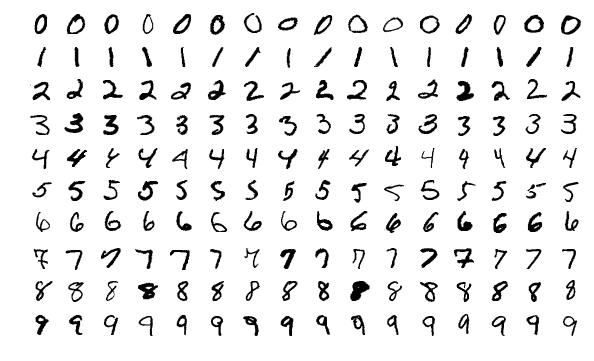
\includegraphics[width=.8\textwidth]{figuras/MNIST_ex.jpg}
    \caption{Amostra de imagens do dataset MNIST. Fonte: \cite{wikipedia_mnist}}
    \label{fig:mnist}
\end{figure}


A importância do MNIST no contexto de aprendizado de máquina reside em sua capacidade de fornecer um benchmark robusto para avaliar o desempenho de algoritmos de classificação. Devido à sua simplicidade relativa, ele permite que pesquisadores e praticantes explorem novas técnicas de aprendizado de forma rápida e eficaz, proporcionando um primeiro passo na avaliação de novos métodos antes de aplicá-los em datasets mais complexos.

O objetivo deste experimento é validar a aplicação do nosso algoritmo no contexto de classificação de imagens utilizando o dataset MNIST. Buscamos demonstrar que o algoritmo é capaz de alcançar um tempo de aprendizado e erro aceitáveis, mesmo quando treinado com um número limitado de imagens. Essa característica é especialmente relevante porque, ao contrário das redes neurais profundas, que apesar de seu poder de generalização, frequentemente exigem grandes quantidades de dados de treinamento e produzem resultados difíceis de interpretar, o método proposto consegue aprender com menos dados e ainda manter a interpretabilidade.

No decorrer deste experimento, pretendemos mostrar que nosso método não só é eficiente, como também mantém um alto nível de interpretabilidade, permitindo uma compreensão clara do processo de decisão. Essa transparência é um dos principais diferenciais da nossa abordagem, tornando-o uma alternativa atraente em cenários onde a explicabilidade do modelo é tão importante quanto sua precisão.

\subsection{Aprendizado do WOMC}

Para avaliar o método no contexto de classificação de imagens, realizamos o aprendizado com foco no dígito 1 utilizando uma configuração com 7 camadas ($n=7$) e janelas 5x5 ($d_{W} = 5$). Podemos ver que este é o experimento de maior complexidade computacional. Para esse experimento utilizamos duas configurações de dados, ambas com baixíssimas quantidade, comparadas ao tamanho total do dataset (60.000 imagens). Primeiro como dados de treinamento mantivemos fixos 100 imagens ($N = 100$), sendo que delas 33 eram o dígito 1 e 67 eram os demais dígitos, selecionado de forma aleatória. Já para os dados de validação para o teste 1 foram selecionadas 100 imagens e para o teste 2, 500 imagens de validação ($M = 100 \ \text{ou} \ 500$), sendo elas 33 ou 100, respectivamente, do dígito 1. A ideia desses experimentos é testar a capacidade de aprendizado com poucos dados, tarefa de maior complexidade quando falamos de redes neurais modernas. O experimento $1b$ com mais imagens de validação consiste em ajudar o algoritmo na seleção da melhor configuração de janelas, quando comparado ao $1a$. 

Os demais parâmetros do algoritmo foram constantes nos dois experimentos: utilizamos 10 vizinhos amostrados para o reticulado das funções características ($r=10$) e 20 vizinhos para o reticulado das janelas ($s=20$); o aprendizado da função característica ocorreu ao longo de 500 épocas ($Epoch_f = 500$) e o aprendizado da janela ao longo de 30 épocas ($Epoch_w = 30$); utilizou-se um tamanho de batch de 50 ($b=50$), com critério de early stopping para o reticulado da função após 50 épocas ($es_{f} = 50$) e para o reticulado da janela após 10 épocas ($es_{w} = 10$). A janela inicial foi configurada em cruz ($W_{ini} = [[0,0,0,0,0],[0,0,1,0,0],[0,1,1,1,0],[0,0,1,0,0],[0,0,0,0,0]]$).

%Apesar da baixíssima quantidade de dados, atingimos erro de treino $L_{t} = 0.0100$ e de validação de $L_{v} = 0.0100$ na época 26 após 440 minutos. O treino total ficou em 653 minutos e o erro no dataset completo de teste do MNIST (10.000 imagens) ficou em $L_{tt} = 0.0762$.

Os resultados desses experimentos encontram-se na Tabela \ref{tab:resultados_mnist} onde os erros de teste ficaram em 0.0762 para a \textit{Run} 1 e 0.0317 para a \textit{Run} 2. Resultados acima da expectativa dada a baixa quantidade de dados de treinamento e a baixa quantidade de épocas utilizadas.

A Figura \ref{fig:confusion_matrix}  apresenta as matrizes de confusão obtida após o treinamento utilizando os dados de teste. Esta matriz é uma ferramenta essencial para avaliar a performance do modelo de classificação, indicando como as previsões se alinham com os valores reais.

Na matriz, o campo \textbf{Verdadeiros Negativos (0,0)} mostra que 97\% dos exemplos que não representam o dígito 1 foram corretamente classificados como não sendo o dígito 1 no experimento 2 e 93\% no experimento 1. O campo \textbf{Falsos Positivos (0,1)} indica que 3\% desses exemplos foram incorretamente classificados como o dígito 1 no experimento 2 e 7\% no experimento 1. Já o campo \textbf{Falsos Negativos (1,0)} revela que 4\% dos exemplos que representam o dígito 1 foram incorretamente classificados como não sendo o dígito 1 no experimento 2 e 9\% no experimento 1. Por fim, o campo \textbf{Verdadeiros Positivos (1,1)} mostra que 96\% dos exemplos do dígito 1 foram corretamente identificados como o dígito 1 no experimento 2 e 91\% no experimento 1.

Esses resultados indicam que mesmo com uma baixíssima quantidade de dados, o modelo possui alta precisão na identificação do dígito 1, com baixas taxas de erro, o que demonstra sua eficácia na tarefa de classificação.

\begin{figure}
  \centering

  \begin{subfigure}{0.49\textwidth}
    \centering
    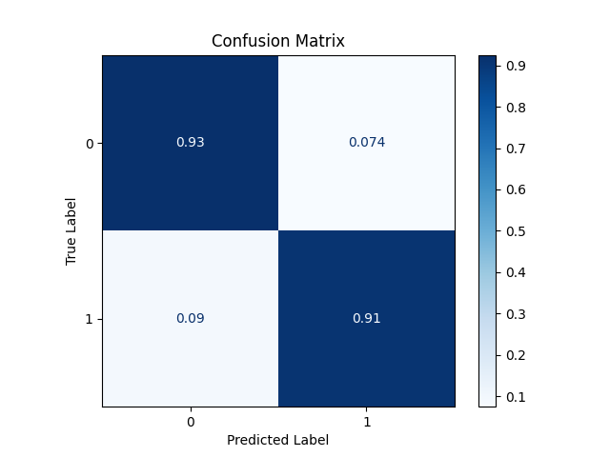
\includegraphics[width=1.1\textwidth]{figuras/conf_matrix_100.png}
    \caption{Matriz de confusão do experimento $1$ ($M=100$).\label{fig:subfig:conf1}}
  \end{subfigure}
  \begin{subfigure}{0.49\textwidth}
    \centering
      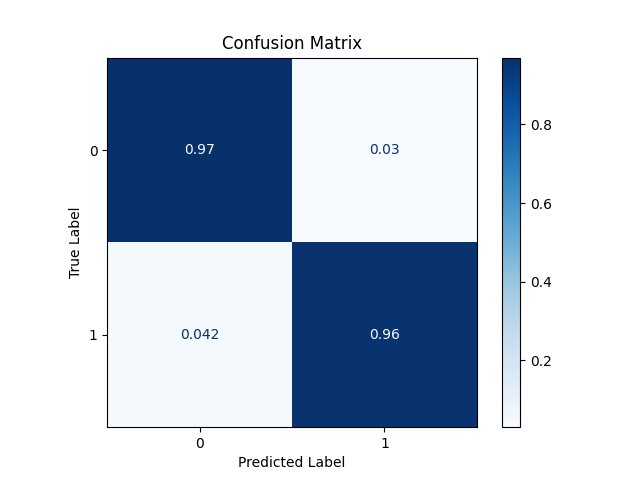
\includegraphics[width=1.1\textwidth]{figuras/conf_matrix.png}
    \caption{Matriz de confusão do experimento $2$ ($M=500$)\label{fig:subfig:conf2}}
  \end{subfigure}

  \caption{Matriz de Confusão para os experimentos de aprendizado do WOMC no contexto de classificação do dígito 1.\label{fig:confusion_matrix}}
\end{figure}

Nas Figuras \ref{fig:painel_acerto} e \ref{fig:painel_erro}, podemos observar o comportamento do W-operador final aprendido, analisando seu funcionamento em cada camada e o resultado final, com o último bit correspondente à classificação. A Figura \ref{fig:painel_acerto} exibe o painel dos acertos, enquanto a Figura \ref{fig:painel_erro} apresenta o painel dos erros. A partir da análise detalhada de cada W-operador em cada camada e dos resultados representados nesses painéis, é possível inferir o processo de classificação do modelo. Esta etapa é crucial para avaliar a interpretabilidade do modelo, permitindo compreender como as decisões de classificação estão sendo tomadas.

\begin{figure}[H]
    \centering
    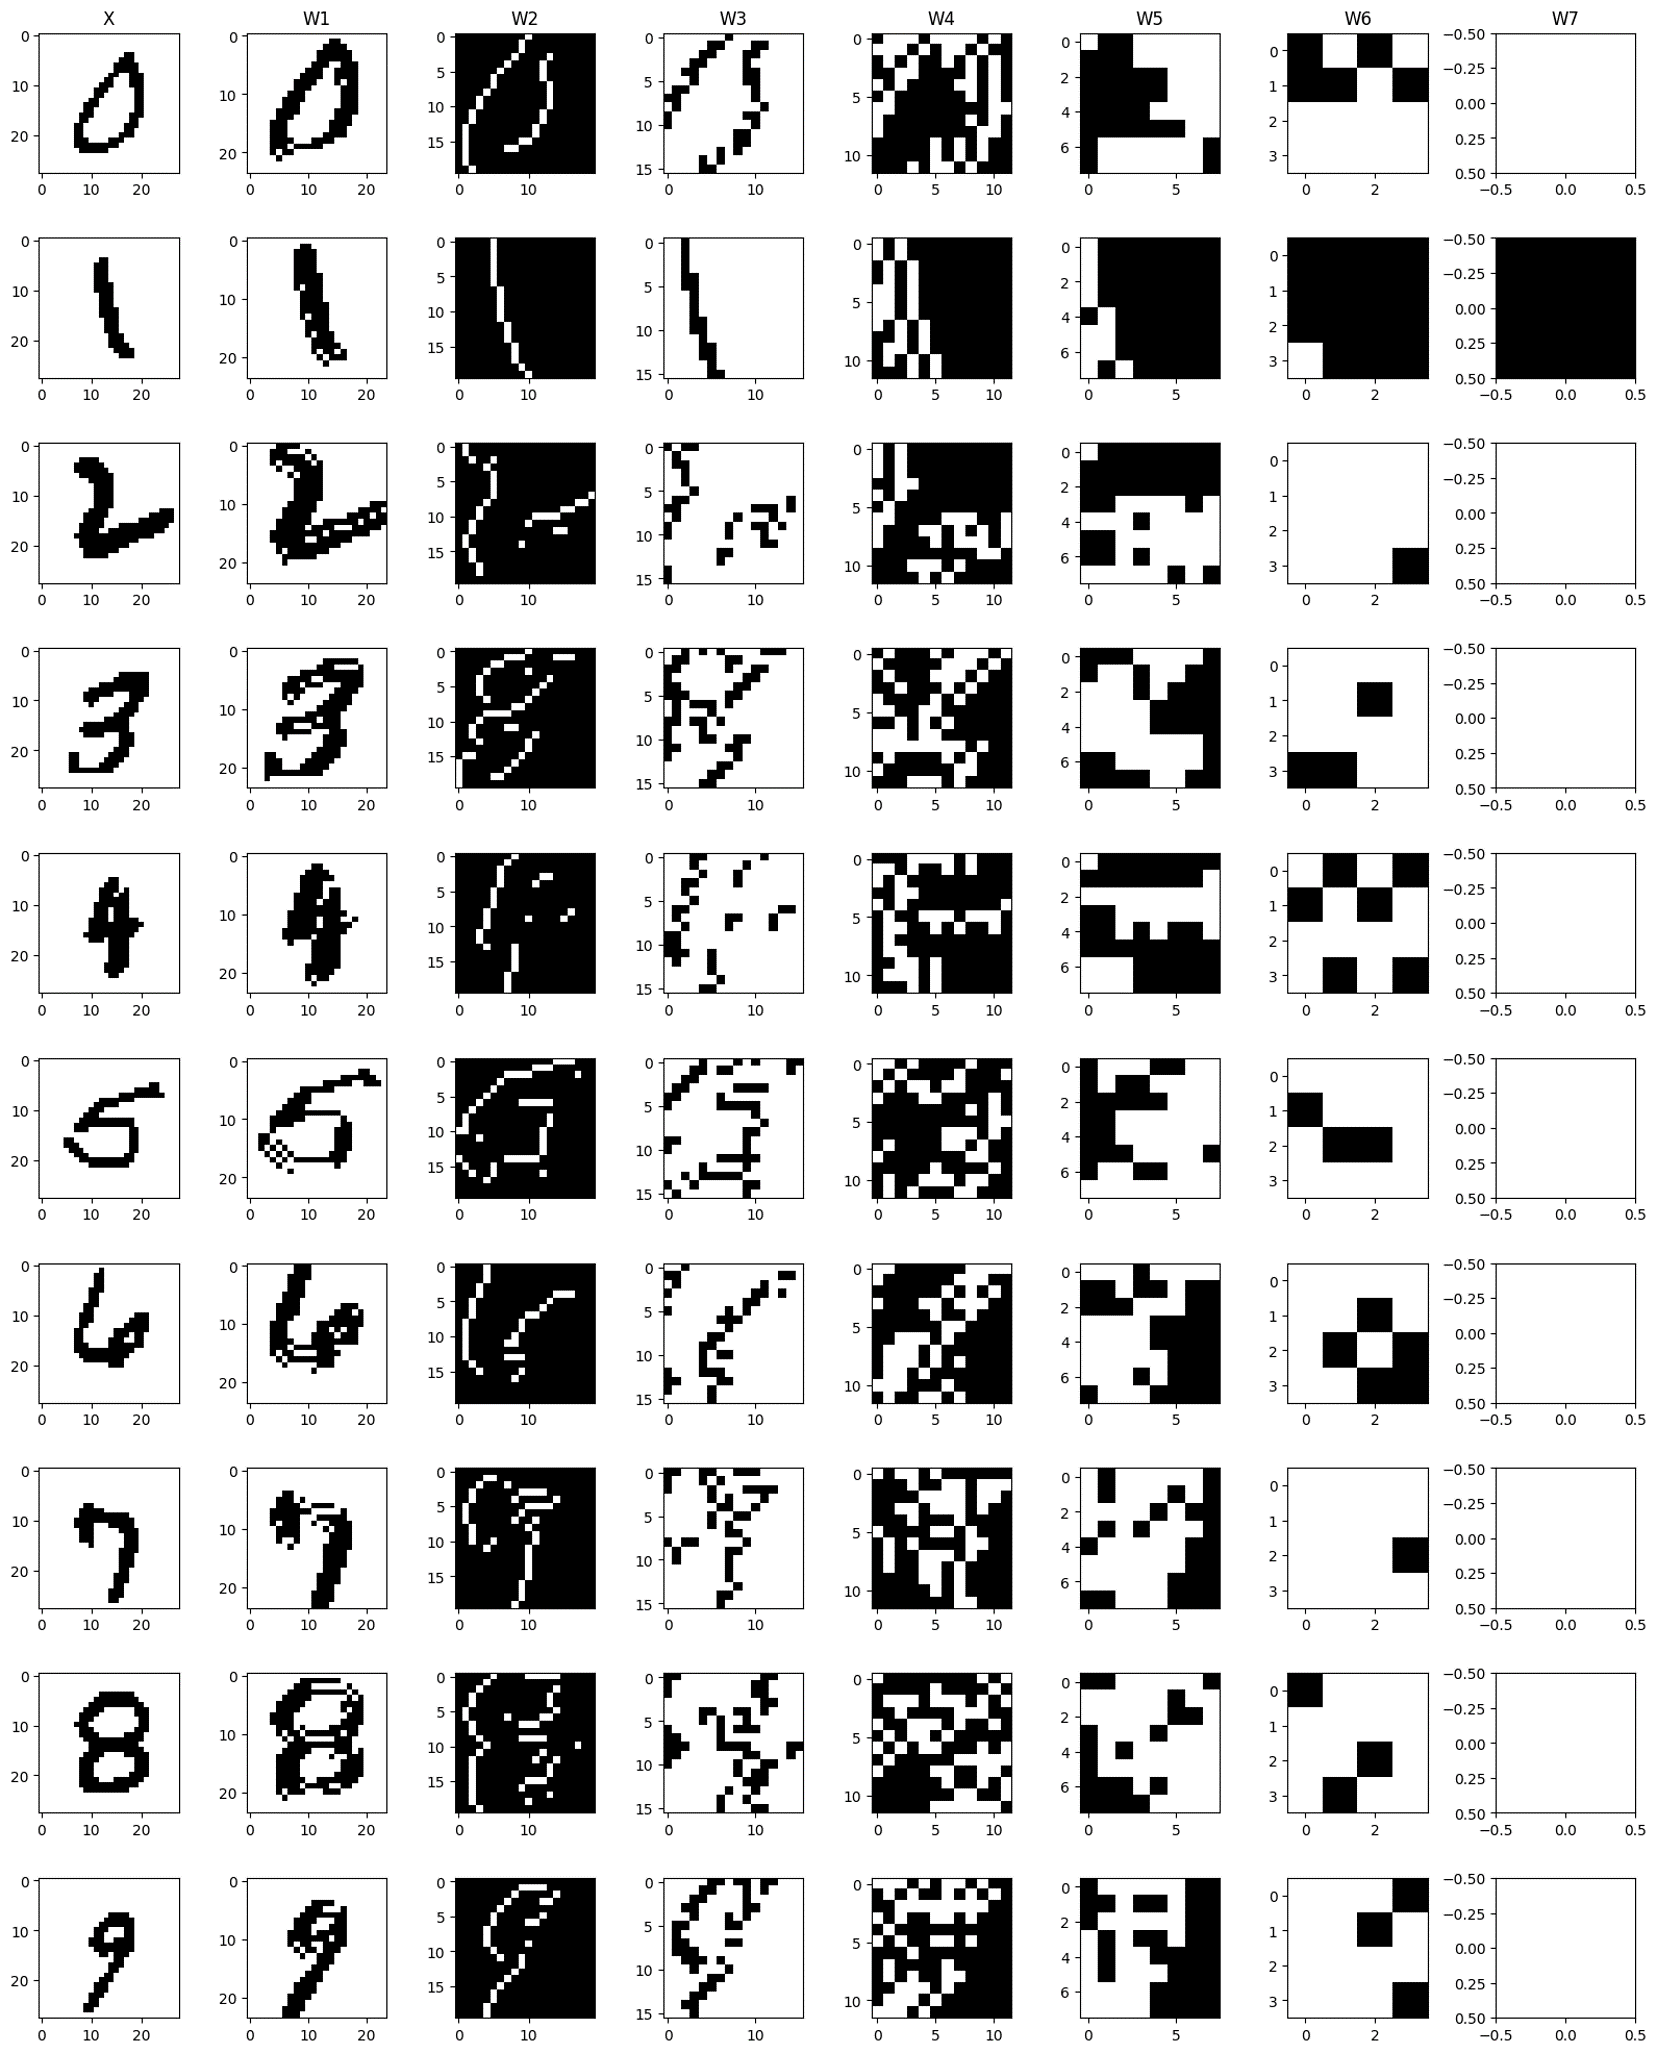
\includegraphics[width=0.5\textwidth]{figuras/painel_acerto.png}
    \caption{Painel de imagens classificadas corretamente.}
    \label{fig:painel_acerto}
\end{figure}

\begin{figure}[H]
    \centering
    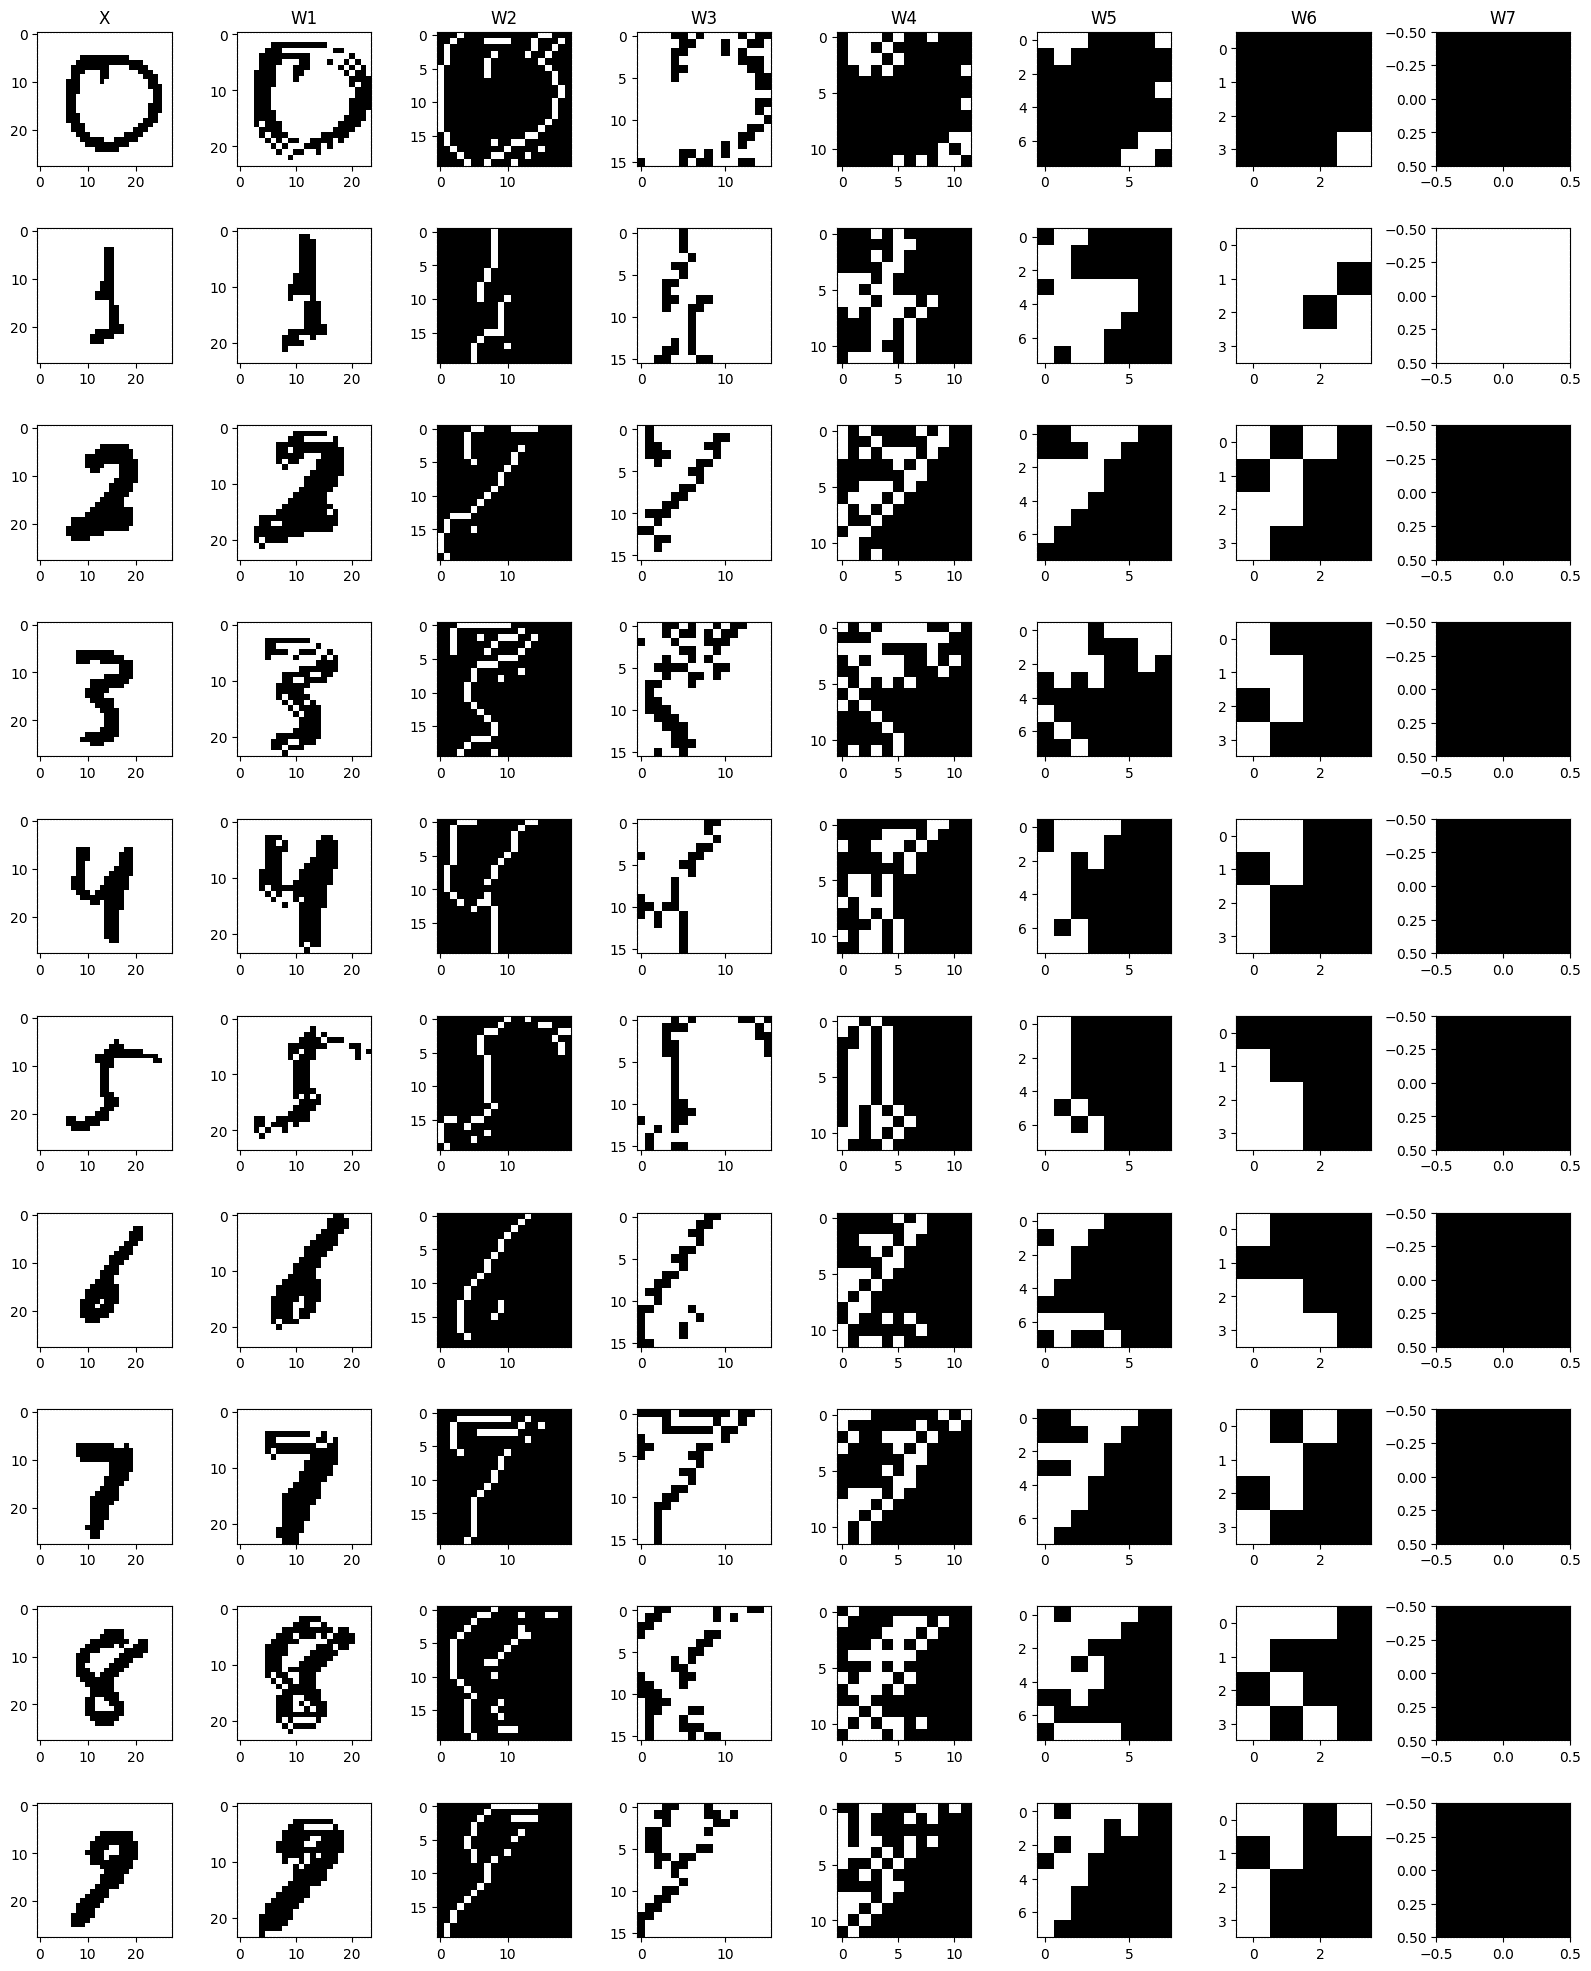
\includegraphics[width=0.5\textwidth]{figuras/painel_erro.png}
    \caption{Painel de imagens classificadas incorretamente.}
    \label{fig:painel_erro}
\end{figure}

\subsection{Aprendizado com Rede Neural}

Para fins de comparação, treinamos o conjunto de dados MNIST utilizando uma rede neural convolucional (CNN) para a tarefa de classificação de imagens. A descrição completa da configuração dessa rede encontra-se no Apêndice \ref{apsec:cnn}.  (\textit{early stop} = quantidade de épocas).

Na primeira parte do experimento, seguimos a metodologia tradicional, utilizando todas as 60.000 imagens de treino e avaliando o erro nas 10.000 imagens do conjunto de teste. Com um batch size de 256 e apenas 10 épocas de treinamento, a rede neural alcançou um erro no conjunto de teste de 0.0015, como esperado para esse tipo de modelo. Esse teste foi realizado para comprovar a eficiência da arquitetura utilizada para a comparação

Na segunda parte do experimento temos o objetivo de comparar os métodos WOMC e CNN. A arquitetura da CNN utiliza dados de validação não durante o treinamento, mas como critério de \textit{early stop}, para garantir a justa comparação entre os métodos utilizamos sempre a quantidade de amostra de treinamento igual a soma da amostra de treino e validação no método WOMC e removemos o critério de \textit{early stop}. Foram realizados 2 experimentos então, as \textit{Runs} 3 e 4 a serem comparadas com as \textit{Runs} 1 e 2, com as mesmas 200 e 600 imagens treinadas nos experimento do WOMC, respectivamente. O experimento foi realizado com 100 épocas de treinamento e \textit{batch} de 50. O erro final no conjunto de teste foi de 0.8857 para a \textit{Run} 3 e de 0.0043 para a \textit{Run} 4, evidenciando que a rede neural não conseguiu aprender e generalizar de forma eficiente com a arquitetura empregada, especialmente com a quantidade limitada de apenas 200 imagens. Em contraste, ao utilizar 600 imagens, a CNN demonstrou uma capacidade de generalização superior em comparação ao método WOMC.

\subsection{Resultados}

A tabela \ref{tab:resultados_mnist} apresenta os resultados compilados dos experimentos mencionados acima com o aprendizado do WOMC nos experimentos 1 e 2 com $M=100$ e $M=500$ respectivamente e dos experimentos com a CNN nos experimentos 3 e 4 com $N=200$ e $N=600$.

\begin{table}[ht]
    \centering
    \resizebox{\textwidth}{!}{ % Redimensiona a tabela para caber na largura da página
        \begin{tabular}{cccccccccc}
            \toprule
            $R$ & Método & $N$ & $M$ & $L_{t}$ & $L_{v}$ & $L_{tt}$ & $Epoch_{W_{min}}$ & $t_{total} \ (min)$ & $t_{Epoch_{min}} \ (min)$ \\
            \midrule
            1 & WOMC & 100 & 100 & 0.0100 & 0.0100 & 0.0762 & 26 & 653 & 440 \\
            2 & WOMC & 100 & 500 & 0.0050 & 0.0180 & 0.0317 & 21 & 792 & 473 \\
            3 & CNN  & 200 & 100 & 0.6700 & 0.6600 & 0.8865 & 55 & 2 & 4 \\
            4 & CNN  & 600 & 100 & 0.0117 & 0.0500 & 0.0043 & 63 & 6 & 10 \\
            \bottomrule
        \end{tabular}
    }
    \caption[Resultados dos experimentos MNIST Dataset]{Resultados dos experimentos para a classificação do dígito 1, utilizando os métodos WOMC e CNN, com as diferentes configurações de tamanho de dataset de treino e validação. São apresentados os erros de treino, validação e teste, a época com erro de validação mínimo, o tempo total e o tempo para o erro de validação mínimo.}
    \label{tab:resultados_mnist}
\end{table}
%!TeX root=../tese.tex
%("dica" para o editor de texto: este arquivo é parte de um documento maior)
% para saber mais: https://tex.stackexchange.com/q/78101

\newcommand{\up}[1]{\raisebox{1.5ex}[0pt]{#1}}

\chapter{Conclusão}
\label{chap:conclusao}

 Neste trabalho estudamos o aprendizado de W-operadores multicamadas nos contextos de transformação e classificação de imagens. Na Seção \ref{sec:resumo_conclusao}, mostramos as principais contribuições deste trabalho. Na Seção \ref{sec:futuro}, propomos ideias e sugestões para melhoria e continuidade da pesquisa realizada neste trabalho.

\section{Resumo das Principais Contribuições}
\label{sec:resumo_conclusao}

Esta dissertação apresentou diversas contribuições significativas para o campo da Morfologia Matemática e o aprendizado de W-operadores multicamadas. As principais contribuições deste trabalho são as seguintes:

\begin{enumerate}
    \item \textbf{Desenvolvimento do Algoritmo descendente no reticulado para o Aprendizado de W-Operadores Multicamadas:} Implementamos um algoritmo descendente no reticulado inovador que percorre um Learning Space Booleano, possibilitando o aprendizado simultâneo das janelas e funções características de W-operadores multicamadas. Esse avanço contribui para a teoria do aprendizado de composições de W-operadores, oferecendo uma abordagem eficiente e robusta para a filtragem e classificação de imagens binárias.

    \item \textbf{Integração de Técnicas de Vetorização de dados em GPU e Exploração Estocástica:} O algoritmo desenvolvido incorporou técnicas de vetorização de dados em GPU e exploração estocástica das cadeias do reticulado Booleano, melhorando significativamente a eficiência computacional e a capacidade de aprendizado do modelo em cenários complexos.

    \item \textbf{Aplicação a Problemas Reais de Transformação e Classificação de Imagens:} Demonstramos a eficácia do algoritmo proposto ao aplicá-lo a três problemas distintos: a filtragem de imagens binárias, o aprendizado da função de transição do \textit{Conway's Game of Life}, e a classificação de dígitos manuscritos utilizando o dataset MNIST. Esses experimentos validaram a aplicabilidade e a robustez do método em diferentes contextos de processamento de imagens.

    \item \textbf{Contribuição para a Interpretação e Consistência Lógica de Modelos:} Diferentemente de muitos métodos modernos baseados em redes neurais, as hipóteses representadas por W-operadores multicamadas no nosso modelo são altamente interpretáveis e logicamente consistentes. Isso permite uma melhor compreensão das propriedades dos operadores aprendidos, promovendo a transparência e a confiabilidade do processo de aprendizado.
\end{enumerate}

Essas contribuições não apenas avançam o estado da arte na área de Morfologia Matemática, mas também abrem novas possibilidades para o desenvolvimento de algoritmos de aprendizado mais eficientes e interpretáveis em diversas aplicações práticas.

\section{Perspectivas Futuras}
\label{sec:futuro}

Durante a realização dos experimentos, um dos principais desafios enfrentados foi a limitação de memória na GPU, especialmente durante o aprendizado da função característica onde vetorizamos o cálculo do erro de todos os vizinhos de distância 1 do nó atual com a aplicação de todos os W-operadores de todas as camadas em todas as imagens do \textit{batch}. No experimento mais complexo, utilizando o dataset MNIST com 7 camadas 5x5, foi necessário remover a vetorização das camadas devido à incapacidade da GPU de calcular todos os vizinhos de todas as camadas simultaneamente. Essa limitação comprometeu drasticamente o desempenho em termos de tempo, o que impactou a eficiência do algoritmo na exploração de caminhos no reticulado Booleano.

Para superar esse desafio, futuras pesquisas podem focar na otimização do uso de memória e/ou na utilização de múltiplas GPUs em paralelo, o que poderia reduzir significativamente o tempo de execução e permitir a exploração de mais caminhos no reticulado, especialmente em experimentos de alta complexidade como o do MNIST. 

Outra possível melhoria seria a paralelização do cálculo dos vizinhos de cada janela. Dado que os cálculos dos vizinhos são independentes entre si, essa abordagem permitiria realizar essas operações simultaneamente, com a tomada de decisão sobre qual vizinho saltar sendo feita apenas após todos os resultados estarem disponíveis. Essas melhorias representam potenciais evoluções do trabalho desenvolvido nesta dissertação e abrem caminho para futuras investigações nesse campo.


%%%%%%%%%%%%%%%%%%%%%%%%%%%% APÊNDICES E ANEXOS %%%%%%%%%%%%%%%%%%%%%%%%%%%%%%%%

% Um apêndice é algum conteúdo adicional de sua autoria que faz parte e
% colabora com a ideia geral do texto mas que, por alguma razão, não precisa
% fazer parte da sequência do discurso; por exemplo, a demonstração de um
% teorema intermediário, as perguntas usadas em uma pesquisa qualitativa etc.
%
% Um anexo é um documento que não faz parte da tese (em geral, nem é de sua
% autoria) mas é relevante para o conteúdo; por exemplo, a especificação do
% padrão técnico ou a legislação que o trabalho discute, um artigo de jornal
% apresentando a percepção do público sobre o tema da tese etc.
%
% Os comandos appendix e annex reiniciam a numeração de capítulos e passam
% a numerá-los com letras. "annex" não faz parte de nenhuma classe padrão,
% foi criado para este modelo. Se o trabalho não tiver apêndices ou anexos,
% remova estas linhas.
%
% Diferentemente de \mainmatter, \backmatter etc., \appendix e \annex não
% forçam o início de uma nova página. Em geral isso não é importante, pois
% o comando seguinte costuma ser "\chapter", mas pode causar problemas com
% a formatação dos cabeçalhos. Assim, vamos forçar uma nova página antes
% de cada um deles.

%%%% Apêndices %%%%

\cleardoublepage

\pagestyle{appendix}

\appendix

% \addappheadtotoc acrescenta a palavra "Apêndice" ao sumário; se
% só há apêndices, sem anexos, provavelmente não é necessário.
\addappheadtotoc

%!TeX root=../tese.tex
%("dica" para o editor de texto: este arquivo é parte de um documento maior)
% para saber mais: https://tex.stackexchange.com/q/78101

\chapter{Anexos aos Experimentos}
\label{ap:results}

\section{Reconhecimento de bordas de dígitos com ruído}
\label{apsec:reslts_digits}

\subsection{Resultados Completos}

Na Tabela \ref{tab:ap_resultados_runs_digitos}, apresentamos todos os resultados conforme apresentado na seção \ref{sec:app_digitos}. A tabela inclui os erros de treinamento ($L_{t}$), validação ($L_{v}$) e teste ($L_{tt}$) utilizando a notação "Valor Mínimo - Valor Médio (Desvio Padrão)". O erro de teste foi calculado ao final de cada execução sem interferência alguma nos treinamentos executados. Na tabela também temos a mínima época ($Epoch_{W_{min}}$ - época que obteve o menor erro de validação), os tempos em minutos de execução total de cada \textit{run} ($t_{total}$),  e o tempo para a mínima época ($t_{Epoch_{min}}$), estes com a notação "Valor Mínimo - Valor Médio (Desvio Padrão)". Na Tabela \ref{tab:ap_hiperparametros_run} temos as configurações dos hiperparâmetros para cada uma das \textit{runs}. 

\begin{table}[ht]
    \centering
    \resizebox{\textwidth}{!}{ % Redimensiona a tabela para caber na largura da página
        \begin{tabular}{ccccccc}
            \toprule
            $R$ & $L_{t}$ & $L_{v}$ & $L_{tt}$ & $Epoch_{W_{min}}$ & $t_{total} \ (min)$ & $t_{Epoch_{min}} \ (min)$ \\
            \midrule
            0 & 0.0151 - 0.0314 (0.0223) & 0.0262 - 0.0404 (0.0217) & 0.0200 - 0.0238 (0.0036) & 4 - 22 (15) & 5.19 - 9.05 (2.07) & 0.90 - 4.91 (3.28) \\
            1 & 0.0129 - 0.0727 (0.1453) & 0.0237 - 0.0809 (0.1420) & 0.0123 - 0.0209 (0.0035) & 14 - 26 (10) & 7.53 - 9.39 (1.08) & 2.56 - 5.23 (2.22) \\
            2 & 0.0129 - 0.0374 (0.0387) & 0.0217 - 0.0457 (0.0379) & 0.0111 - 0.0208 (0.0045) & 6 - 21 (9) & 3.36 - 5.04 (0.72) & 0.81 - 2.57 (1.07) \\
            3 & 0.0138 - 0.0727 (0.1374) & 0.0258 - 0.0813 (0.1340) & 0.0195 - 0.0245 (0.0042) & 12 - 27 (13) & 3.99 - 5.20 (0.53) & 1.27 - 3.10 (1.42) \\
            4 & 0.0124 - 0.0290 (0.0212) & 0.0230 - 0.0376 (0.0207) & 0.0111 - 0.0203 (0.0042) & 9 - 27 (12) & 8.62 - 14.62 (2.22) & 3.22 - 8.69 (3.43) \\
            5 & 0.0130 - 0.0708 (0.1485) & 0.0235 - 0.0793 (0.1450) & 0.0146 - 0.0209 (0.0035) & 13 - 25 (12) & 8.33 - 14.76 (2.67) & 3.57 - 8.22 (4.64) \\
            6 & 0.0126 - 0.0320 (0.0351) & 0.0220 - 0.0406 (0.0343) & 0.0112 - 0.0213 (0.0043) & 24 - 35 (8) & 8.99 - 9.94 (0.75) & 4.86 - 7.08 (1.59) \\
            7 & 0.0134 - 0.0647 (0.1381) & 0.0251 - 0.0739 (0.1346) & 0.0189 - 0.0212 (0.0014) & 16 - 25 (8) & 7.65 - 9.66 (1.53) & 2.88 - 4.93 (2.07) \\
            8 & 0.0132 - 0.0307 (0.0312) & 0.0246 - 0.0403 (0.0298) & 0.0188 - 0.0216 (0.0019) & 12 - 24 (10) & 9.05 - 12.04 (1.93) & 3.72 - 6.83 (2.54) \\
            9 & 0.0125 - 0.0658 (0.1408) & 0.0222 - 0.0748 (0.1374) & 0.0116 - 0.0210 (0.0045) & 22 - 30 (7) & 9.64 - 11.28 (0.77) & 4.41 - 6.65 (1.64) \\
            10 & 0.0126 - 0.0356 (0.0340) & 0.0257 - 0.0448 (0.0327) & 0.0180 - 0.0220 (0.0036) & 9 - 30 (13) & 4.14 - 6.35 (1.21) & 1.22 - 4.14 (1.93) \\
            11 & 0.0118 - 0.0656 (0.1363) & 0.0258 - 0.0757 (0.1326) & 0.0170 - 0.0222 (0.0035) & 13 - 29 (12) & 5.31 - 6.74 (0.62) & 1.53 - 4.06 (1.81) \\
            12 & 0.0123 - 0.0260 (0.0306) & 0.0220 - 0.0359 (0.0292) & 0.0128 - 0.0192 (0.0030) & 5 - 31 (12) & 10.58 - 20.73 (3.20) & 1.99 - 13.91 (5.57) \\
            13 & 0.0094 - 0.0649 (0.1436) & 0.0217 - 0.0738 (0.1402) & 0.0104 - 0.0178 (0.0040) & 18 - 28 (8) & 11.46 - 15.19 (1.39) & 4.77 - 8.52 (2.67) \\
            14 & 0.0113 - 0.0331 (0.0349) & 0.0213 - 0.0420 (0.0338) & 0.0129 - 0.0188 (0.0030) & 8 - 29 (13) & 5.71 - 9.04 (1.75) & 1.84 - 5.89 (2.94) \\
            15 & 0.0113 - 0.0615 (0.1369) & 0.0244 - 0.0711 (0.1333) & 0.0155 - 0.0199 (0.0025) & 12 - 28 (11) & 6.97 - 10.13 (1.24) & 1.72 - 5.68 (2.44) \\
            16 & 0.0205 - 0.0371 (0.0297) & 0.0216 - 0.0384 (0.0292) & 0.0125 - 0.0152 (0.0017) & 12 - 30 (10) & 10.25 - 13.79 (1.53) & 3.51 - 8.64 (2.95) \\
            17 & 0.0185 - 0.0757 (0.1405) & 0.0224 - 0.0775 (0.1397) & 0.0121 - 0.0167 (0.0023) & 13 - 29 (10) & 8.69 - 12.73 (1.91) & 2.63 - 7.45 (3.15) \\
            18 & 0.0220 - 0.0424 (0.0397) & 0.0239 - 0.0440 (0.0392) & 0.0135 - 0.0172 (0.0019) & 7 - 21 (11) & 4.99 - 7.95 (1.65) & 1.34 - 4.09 (2.09) \\
            19 & 0.0200 - 0.0764 (0.1344) & 0.0237 - 0.0788 (0.1334) & 0.0137 - 0.0186 (0.0033) & 12 - 32 (15) & 5.39 - 8.29 (1.36) & 1.56 - 5.41 (2.71) \\
            20 & 0.0202 - 0.0333 (0.0300) & 0.0214 - 0.0346 (0.0295) & 0.0134 - 0.0156 (0.0015) & 8 - 25 (10) & 12.66 - 20.93 (3.30) & 3.23 - 11.90 (4.69) \\
            21 & 0.0183 - 0.0678 (0.1379) & 0.0208 - 0.0691 (0.1372) & 0.0123 - 0.0151 (0.0022) & 20 - 36 (9) & 19.90 - 21.84 (1.34) & 8.05 - 15.72 (4.50) \\
            22 & 0.0209 - 0.0378 (0.0377) & 0.0217 - 0.0388 (0.0372) & 0.0124 - 0.0170 (0.0037) & 14 - 27 (11) & 11.06 - 15.26 (2.24) & 4.51 - 9.38 (3.95) \\
            23 & 0.0194 - 0.0705 (0.1349) & 0.0228 - 0.0731 (0.1339) & 0.0130 - 0.0173 (0.0021) & 12 - 28 (12) & 8.31 - 13.20 (2.95) & 2.17 - 7.66 (4.05) \\
            24 & 0.0173 - 0.0352 (0.0314) & 0.0203 - 0.0373 (0.0307) & 0.0110 - 0.0158 (0.0030) & 12 - 34 (12) & 14.09 - 18.55 (2.22) & 4.82 - 12.92 (4.59) \\
            25 & 0.0177 - 0.0708 (0.1398) & 0.0209 - 0.0729 (0.1389) & 0.0101 - 0.0156 (0.0030) & 20 - 33 (10) & 14.23 - 16.91 (1.49) & 5.32 - 11.00 (4.19) \\
            26 & 0.0205 - 0.0380 (0.0304) & 0.0214 - 0.0399 (0.0300) & 0.0115 - 0.0196 (0.0033) & 16 - 23 (5) & 7.57 - 9.28 (0.86) & 3.41 - 4.85 (0.97) \\
            27 & 0.0190 - 0.0689 (0.1347) & 0.0220 - 0.0718 (0.1336) & 0.0137 - 0.0174 (0.0024) & 19 - 25 (4) & 8.81 - 10.07 (0.77) & 3.52 - 5.10 (0.97) \\
            28 & 0.0171 - 0.0309 (0.0302) & 0.0198 - 0.0332 (0.0296) & 0.0104 - 0.0146 (0.0017) & 15 - 29 (10) & 19.92 - 27.70 (3.77) & 8.95 - 17.16 (6.07) \\
            29 & 0.0181 - 0.0674 (0.1405) & 0.0196 - 0.0697 (0.1395) & 0.0123 - 0.0145 (0.0018) & 14 - 37 (12) & 15.96 - 26.21 (4.55) & 4.80 - 19.49 (7.77) \\
            30 & 0.0199 - 0.0353 (0.0304) & 0.0211 - 0.0373 (0.0301) & 0.0126 - 0.0177 (0.0033) & 4 - 23 (13) & 8.68 - 13.99 (2.49) & 1.18 - 7.63 (4.32) \\
            31 & 0.0195 - 0.0716 (0.1394) & 0.0227 - 0.0740 (0.1385) & 0.0128 - 0.0161 (0.0015) & 13 - 21 (7) & 9.60 - 13.53 (2.63) & 2.94 - 6.32 (2.54) \\
            32 & 0.0254 - 0.0330 (0.0278) & 0.0286 - 0.0373 (0.0259) & 0.0211 - 0.0223 (0.0010) & 5 - 18 (11) & 5.57 - 8.10 (1.68) & 0.90 - 3.69 (2.36) \\
            33 & 0.0255 - 0.0796 (0.1610) & 0.0291 - 0.0836 (0.1596) & 0.0204 - 0.0219 (0.0009) & 7 - 23 (15) & 5.14 - 7.92 (1.71) & 0.67 - 4.00 (2.96) \\
            34 & 0.0255 - 0.0356 (0.0292) & 0.0291 - 0.0398 (0.0273) & 0.0201 - 0.0218 (0.0011) & 3 - 12 (7) & 2.09 - 3.22 (0.75) & 0.34 - 1.14 (0.67) \\
            35 & 0.0255 - 0.0751 (0.1397) & 0.0286 - 0.0790 (0.1382) & 0.0204 - 0.0215 (0.0007) & 9 - 22 (12) & 2.48 - 4.06 (0.91) & 0.67 - 2.07 (1.25) \\
            36 & 0.0247 - 0.0384 (0.0294) & 0.0284 - 0.0417 (0.0276) & 0.0208 - 0.0235 (0.0019) & 4 - 16 (9) & 9.52 - 14.38 (3.17) & 1.61 - 5.91 (3.58) \\
            37 & 0.0258 - 0.0506 (0.0333) & 0.0286 - 0.0533 (0.0316) & 0.0202 - 0.0238 (0.0041) & 3 - 13 (8) & 6.35 - 9.17 (1.99) & 0.63 - 3.30 (2.06) \\
            \bottomrule
        \end{tabular}
    }
     \caption[\textit{Runs} do experimento de reconhecimento de bordas de dígitos com ruído]{\textit{Runs} do experimento de reconhecimento de bordas de dígitos com ruído, cada uma com 10 execuções com \textit{seeds} diferentes, erros IoU de treino, validação e teste, época que atingiu o menor erro de validação e tempos total e para atingir o menor erro de validação,  calculados sob essas 10 execuções, no formato "Valor mínimo - Valor médio (desvio padrão)"}
    \label{tab:ap_resultados_runs_digitos}
\end{table}

\begin{table}[ht]
    \centering
    %\resizebox{\textwidth}{!}{ % Redimensiona a tabela para caber na largura da página
        \begin{tabular}{ccccccccccccc}
            \toprule
            $R$ & $n$ & $d_{w}$ & $N$ & $M$ & $r$ & $s$ & $Epoch_f$ & $Epoch_w$ & $b$ & $es_{f}$ & $es_{w}$ & $W_{ini}$ \\
            \midrule
            0 & 2 & 3 & 10 & 10 & 8 & 5 & 100 & 50 & 5 & 30 & 20 & Cruz \\
            1 & 2 & 3 & 10 & 10 & 8 & 5 & 100 & 50 & 5 & 30 & 20 & Centro \\
            2 & 2 & 3 & 10 & 10 & 8 & 5 & 100 & 50 & 10 & 30 & 20 & Cruz \\
            3 & 2 & 3 & 10 & 10 & 8 & 5 & 100 & 50 & 10 & 30 & 20 & Centro \\
            4 & 2 & 3 & 10 & 10 & 8 & 9 & 100 & 50 & 5 & 30 & 20 & Cruz \\
            5 & 2 & 3 & 10 & 10 & 8 & 9 & 100 & 50 & 5 & 30 & 20 & Centro \\
            6 & 2 & 3 & 10 & 10 & 8 & 9 & 100 & 50 & 10 & 30 & 20 & Cruz \\
            7 & 2 & 3 & 10 & 10 & 8 & 9 & 100 & 50 & 10 & 30 & 20 & Centro \\
            8 & 2 & 3 & 10 & 10 & 16 & 5 & 100 & 50 & 5 & 30 & 20 & Cruz \\
            9 & 2 & 3 & 10 & 10 & 16 & 5 & 100 & 50 & 5 & 30 & 20 & Centro \\
            10 & 2 & 3 & 10 & 10 & 16 & 5 & 100 & 50 & 10 & 30 & 20 & Cruz \\
            11 & 2 & 3 & 10 & 10 & 16 & 5 & 100 & 50 & 10 & 30 & 20 & Centro \\
            12 & 2 & 3 & 10 & 10 & 16 & 9 & 100 & 50 & 5 & 30 & 20 & Cruz \\
            13 & 2 & 3 & 10 & 10 & 16 & 9 & 100 & 50 & 5 & 30 & 20 & Centro \\
            14 & 2 & 3 & 10 & 10 & 16 & 9 & 100 & 50 & 10 & 30 & 20 & Cruz \\
            15 & 2 & 3 & 10 & 10 & 16 & 9 & 100 & 50 & 10 & 30 & 20 & Centro \\
            16 & 2 & 3 & 30 & 10 & 8 & 5 & 100 & 50 & 15 & 30 & 20 & Cruz \\
            17 & 2 & 3 & 30 & 10 & 8 & 5 & 100 & 50 & 15 & 30 & 20 & Centro \\
            18 & 2 & 3 & 30 & 10 & 8 & 5 & 100 & 50 & 30 & 30 & 20 & Cruz \\
            19 & 2 & 3 & 30 & 10 & 8 & 5 & 100 & 50 & 30 & 30 & 20 & Centro \\
            20 & 2 & 3 & 30 & 10 & 8 & 9 & 100 & 50 & 15 & 30 & 20 & Cruz \\
            21 & 2 & 3 & 30 & 10 & 8 & 9 & 100 & 50 & 15 & 30 & 20 & Centro \\
            22 & 2 & 3 & 30 & 10 & 8 & 9 & 100 & 50 & 30 & 30 & 20 & Cruz \\
            23 & 2 & 3 & 30 & 10 & 8 & 9 & 100 & 50 & 30 & 30 & 20 & Centro \\
            24 & 2 & 3 & 30 & 10 & 16 & 5 & 100 & 50 & 15 & 30 & 20 & Cruz \\
            25 & 2 & 3 & 30 & 10 & 16 & 5 & 100 & 50 & 15 & 30 & 20 & Centro \\
            26 & 2 & 3 & 30 & 10 & 16 & 5 & 100 & 50 & 30 & 30 & 20 & Cruz \\
            27 & 2 & 3 & 30 & 10 & 16 & 5 & 100 & 50 & 30 & 30 & 20 & Centro \\
            28 & 2 & 3 & 30 & 10 & 16 & 9 & 100 & 50 & 15 & 30 & 20 & Cruz \\
            29 & 2 & 3 & 30 & 10 & 16 & 9 & 100 & 50 & 15 & 30 & 20 & Centro \\
            30 & 2 & 3 & 30 & 10 & 16 & 9 & 100 & 50 & 30 & 30 & 20 & Cruz \\
            31 & 2 & 3 & 30 & 10 & 16 & 9 & 100 & 50 & 30 & 30 & 20 & Centro \\
            32 & 1 & 3 & 30 & 10 & 16 & 9 & 100 & 50 & 15 & 30 & 20 & Cruz \\
            33 & 1 & 3 & 30 & 10 & 16 & 9 & 100 & 50 & 15 & 30 & 20 & Centro \\
            34 & 1 & 3 & 30 & 10 & 16 & 9 & 100 & 50 & 30 & 30 & 20 & Cruz \\
            35 & 1 & 3 & 30 & 10 & 16 & 9 & 100 & 50 & 30 & 30 & 20 & Centro \\
            36 & 1 & 5 & 30 & 10 & 16 & 9 & 100 & 50 & 15 & 30 & 20 & Cruz \\
            37 & 1 & 5 & 30 & 10 & 16 & 9 & 100 & 50 & 30 & 30 & 20 & Cruz \\
            \bottomrule
        \end{tabular}
   % }
    \caption[Configuração de hiperparâmetro das \textit{Runs} do experimento de reconhecimento de bordas de dígitos com ruído]{Configuração de hiperparâmetros de cada \textit{Run}: quantidade de camadas, tamanho da janela, tamanho da amostra de treinamento, tamanho da amostra de validação, quantidade de vizinhos do reticulado da função amostrados, quantidade de vizinhos no reticulado da janela amostrados, quantidade de épocas para o treinamento da função característica, quantidade de épocas para o treinamento da janela, tamanho do \textit{batch}, parâmetros de \textit{early stop} para os aprendizados da função e da janela, respectivamente e janela inicial de treinamento.}
    \label{tab:ap_hiperparametros_run}
\end{table}

\clearpage
\subsection{Funções Características Estimadas}

Nas tabelas \ref{tab:func_w1} e \ref{tab:func_w2} apresentamos as funções características estimadas para os elementos estruturantes apresentados na Figura \ref{fig:WOMC}

\begin{longtable}[c]{rrrrrrr}

%%%%%%%%%%%%
% O cabeçalho da tabela na primeira página em que ela aparece.
\toprule
\multicolumn{6}{c}{Entrada} &
\multicolumn{1}{c}{Saída} \\

\cmidrule(lr){1-6} \cmidrule(lr){7-7}
{$w_1$} &  {$w_2$} &  {$w_3$} &  {$w_4$} &  {$w_5$} &  {$w_6$}& 
{$f$} \\
\cmidrule(lr){1-6} \cmidrule(lr){7-7}


\endfirsthead % Final do cabeçalho que aparece na primeira página

%%%%%%%%%%%%
% O cabeçalho da tabela em todas as páginas em que ela aparece
% exceto a primeira; aqui, igual ao anterior
\toprule
\multicolumn{6}{c}{Entrada} &
\multicolumn{1}{c}{Saída} \\

\cmidrule(lr){1-6} \cmidrule(lr){7-7}
{$w_1$} &  {$w_2$} &  {$w_3$} &  {$w_4$} &  {$w_5$} &  {$w_6$}& 
{$f$} \\
\cmidrule(lr){1-6} \cmidrule(lr){7-7}


\endhead % Final do cabeçalho das páginas seguintes à primeira

%%%%%%%%%%%%
% O rodapé da tabela em todas as páginas em que ela aparece
% exceto a última

\multicolumn{7}{r}{\textit{continua}\enspace$\longrightarrow$}\\

% Como usamos \captionlistentry mais abaixo, usamos "[]" aqui.
\caption[]{Função Característica da Janela $W_{1}$.}

\endfoot % Final do rodapé que aparece em todas as páginas exceto a última

%%%%%%%%%%%%
% O rodapé da tabela na última página em que ela aparece

\bottomrule

% Como usamos \captionlistentry mais abaixo, usamos "[]" aqui.
\caption[]{Função Característica da Janela $W_{1}$.}

\endlastfoot % Final do rodapé da última página

%%%%%%%%%%%%
% O conteúdo da tabela de fato.

% Como a tabela pode se estender por várias páginas, precisamos tomar
% cuidado especial com \caption e \label: se esses comandos forem
% incluídos no cabeçalho ou rodapé que aparece em várias páginas, eles
% serão executados mais de uma vez e tanto a lista de tabelas quanto as
% referências à tabela ficarão incorretas. Há diversas soluções, mas a
% mais simples é (1) não colocar \label no cabeçalho ou rodapé, (2) usar
% "\caption[]" no cabeçalho ou rodapé, que não inclui a tabela na lista
% de tabelas, e (3) colocar \captionlistentry e \label aqui, na primeira
% célula da tabela. \captionlistentry não imprime nada, apenas acrescenta
% um item na lista de tabelas com o número de página correspondente.
\captionlistentry{Função Característica da Janela $W_{1}$.}\label{tab:func_w1}

        0 & 0 & 0 & 0 & 0 & 0 & 0 \\
        0 & 0 & 0 & 0 & 0 & 1 & 0 \\
        0 & 0 & 0 & 0 & 1 & 0 & 0 \\
        0 & 0 & 0 & 0 & 1 & 1 & 0 \\
        0 & 0 & 0 & 1 & 0 & 0 & 0 \\
        0 & 0 & 0 & 1 & 0 & 1 & 0 \\
        0 & 0 & 0 & 1 & 1 & 0 & 0 \\
        0 & 0 & 0 & 1 & 1 & 1 & 0 \\
        0 & 0 & 1 & 0 & 0 & 0 & 0 \\
        0 & 0 & 1 & 0 & 0 & 1 & 0 \\
        0 & 0 & 1 & 0 & 1 & 0 & 0 \\
        0 & 0 & 1 & 0 & 1 & 1 & 1 \\
        0 & 0 & 1 & 1 & 0 & 0 & 0 \\
        0 & 0 & 1 & 1 & 0 & 1 & 1 \\
        0 & 0 & 1 & 1 & 1 & 0 & 1 \\
        0 & 0 & 1 & 1 & 1 & 1 & 1 \\
        0 & 1 & 0 & 0 & 0 & 0 & 0 \\
        0 & 1 & 0 & 0 & 0 & 1 & 0 \\
        0 & 1 & 0 & 0 & 1 & 0 & 0 \\
        0 & 1 & 0 & 0 & 1 & 1 & 0 \\
        0 & 1 & 0 & 1 & 0 & 0 & 0 \\
        0 & 1 & 0 & 1 & 0 & 1 & 0 \\
        0 & 1 & 0 & 1 & 1 & 0 & 0 \\
        0 & 1 & 0 & 1 & 1 & 1 & 1 \\
        0 & 1 & 1 & 0 & 0 & 0 & 0 \\
        0 & 1 & 1 & 0 & 0 & 1 & 1 \\
        0 & 1 & 1 & 0 & 1 & 0 & 1 \\
        0 & 1 & 1 & 0 & 1 & 1 & 1 \\
        0 & 1 & 1 & 1 & 0 & 0 & 1 \\
        0 & 1 & 1 & 1 & 0 & 1 & 1 \\
        0 & 1 & 1 & 1 & 1 & 0 & 1 \\
        0 & 1 & 1 & 1 & 1 & 1 & 1 \\
        1 & 0 & 0 & 0 & 0 & 0 & 0 \\
        1 & 0 & 0 & 0 & 0 & 1 & 0 \\
        1 & 0 & 0 & 0 & 1 & 0 & 0 \\
        1 & 0 & 0 & 0 & 1 & 1 & 0 \\
        1 & 0 & 0 & 1 & 0 & 0 & 0 \\
        1 & 0 & 0 & 1 & 0 & 1 & 0 \\
        1 & 0 & 0 & 1 & 1 & 0 & 0 \\
        1 & 0 & 0 & 1 & 1 & 1 & 0 \\
        1 & 0 & 1 & 0 & 0 & 0 & 1 \\
        1 & 0 & 1 & 0 & 0 & 1 & 1 \\
        1 & 0 & 1 & 0 & 1 & 0 & 1 \\
        1 & 0 & 1 & 0 & 1 & 1 & 1 \\
        1 & 0 & 1 & 1 & 0 & 0 & 1 \\
        1 & 0 & 1 & 1 & 0 & 1 & 1 \\
        1 & 0 & 1 & 1 & 1 & 0 & 1 \\
        1 & 0 & 1 & 1 & 1 & 1 & 1 \\
        1 & 1 & 0 & 0 & 0 & 0 & 0 \\
        1 & 1 & 0 & 0 & 0 & 1 & 0 \\
        1 & 1 & 0 & 0 & 1 & 0 & 0 \\
        1 & 1 & 0 & 0 & 1 & 1 & 1 \\
        1 & 1 & 0 & 1 & 0 & 0 & 0 \\
        1 & 1 & 0 & 1 & 0 & 1 & 1 \\
        1 & 1 & 0 & 1 & 1 & 0 & 0 \\
        1 & 1 & 0 & 1 & 1 & 1 & 1 \\
        1 & 1 & 1 & 0 & 0 & 0 & 1 \\
        1 & 1 & 1 & 0 & 0 & 1 & 1 \\
        1 & 1 & 1 & 0 & 1 & 0 & 1 \\
        1 & 1 & 1 & 0 & 1 & 1 & 1 \\
        1 & 1 & 1 & 1 & 0 & 0 & 1 \\
        1 & 1 & 1 & 1 & 0 & 1 & 1 \\
        1 & 1 & 1 & 1 & 1 & 0 & 1 \\
        1 & 1 & 1 & 1 & 1 & 1 & 1 \\

\end{longtable}

\clearpage
\begin{longtable}[c]{rrrrrrrrr}

%%%%%%%%%%%%
% O cabeçalho da tabela na primeira página em que ela aparece.
\toprule
\multicolumn{8}{c}{Entrada} &
\multicolumn{1}{c}{Saída} \\

\cmidrule(lr){1-8} \cmidrule(lr){9-9}
{$w_1$} &  {$w_2$} &  {$w_3$} &  {$w_4$} &  {$w_5$} &  {$w_6$} &  {$w_7$} &  {$w_8$} & 
{$f$} \\
\cmidrule(lr){1-8} \cmidrule(lr){9-9}


\endfirsthead % Final do cabeçalho que aparece na primeira página

%%%%%%%%%%%%
% O cabeçalho da tabela em todas as páginas em que ela aparece
% exceto a primeira; aqui, igual ao anterior
\toprule
\multicolumn{8}{c}{Entrada} &
\multicolumn{1}{c}{Saída} \\

\cmidrule(lr){1-8} \cmidrule(lr){9-9}
{$w_1$} &  {$w_2$} &  {$w_3$} &  {$w_4$} &  {$w_5$} &  {$w_6$} &  {$w_7$} &  {$w_8$} & 
{$f$} \\
\cmidrule(lr){1-8} \cmidrule(lr){9-9}


\endhead % Final do cabeçalho das páginas seguintes à primeira

%%%%%%%%%%%%
% O rodapé da tabela em todas as páginas em que ela aparece
% exceto a última

\multicolumn{9}{r}{\textit{continua}\enspace$\longrightarrow$}\\

% Como usamos \captionlistentry mais abaixo, usamos "[]" aqui.
\caption[]{Função Característica da Janela $W_{2}$.}

\endfoot % Final do rodapé que aparece em todas as páginas exceto a última

%%%%%%%%%%%%
% O rodapé da tabela na última página em que ela aparece

\bottomrule

% Como usamos \captionlistentry mais abaixo, usamos "[]" aqui.
\caption[]{Função Característica da Janela $W_{2}$.}

\endlastfoot % Final do rodapé da última página

%%%%%%%%%%%%
% O conteúdo da tabela de fato.

% Como a tabela pode se estender por várias páginas, precisamos tomar
% cuidado especial com \caption e \label: se esses comandos forem
% incluídos no cabeçalho ou rodapé que aparece em várias páginas, eles
% serão executados mais de uma vez e tanto a lista de tabelas quanto as
% referências à tabela ficarão incorretas. Há diversas soluções, mas a
% mais simples é (1) não colocar \label no cabeçalho ou rodapé, (2) usar
% "\caption[]" no cabeçalho ou rodapé, que não inclui a tabela na lista
% de tabelas, e (3) colocar \captionlistentry e \label aqui, na primeira
% célula da tabela. \captionlistentry não imprime nada, apenas acrescenta
% um item na lista de tabelas com o número de página correspondente.
\captionlistentry{Função Característica da Janela $W_{2}$.}\label{tab:func_w2}

        0 & 0 & 0 & 0 & 0 & 0 & 0 & 0 & 0 \\
        0 & 0 & 0 & 0 & 0 & 0 & 0 & 1 & 0 \\
        0 & 0 & 0 & 0 & 0 & 0 & 1 & 0 & 0 \\
        0 & 0 & 0 & 0 & 0 & 0 & 1 & 1 & 0 \\
        0 & 0 & 0 & 0 & 0 & 1 & 0 & 0 & 0 \\
        0 & 0 & 0 & 0 & 0 & 1 & 0 & 1 & 1 \\
        0 & 0 & 0 & 0 & 0 & 1 & 1 & 0 & 0 \\
        0 & 0 & 0 & 0 & 0 & 1 & 1 & 1 & 1 \\
        0 & 0 & 0 & 0 & 1 & 0 & 0 & 0 & 0 \\
        0 & 0 & 0 & 0 & 1 & 0 & 0 & 1 & 0 \\
        0 & 0 & 0 & 0 & 1 & 0 & 1 & 0 & 0 \\
        0 & 0 & 0 & 0 & 1 & 0 & 1 & 1 & 0 \\
        0 & 0 & 0 & 0 & 1 & 1 & 0 & 0 & 0 \\
        0 & 0 & 0 & 0 & 1 & 1 & 0 & 1 & 1 \\
        0 & 0 & 0 & 0 & 1 & 1 & 1 & 0 & 0 \\
        0 & 0 & 0 & 0 & 1 & 1 & 1 & 1 & 1 \\
        0 & 0 & 0 & 1 & 0 & 0 & 0 & 0 & 0 \\
        0 & 0 & 0 & 1 & 0 & 0 & 0 & 1 & 1 \\
        0 & 0 & 0 & 1 & 0 & 0 & 1 & 0 & 0 \\
        0 & 0 & 0 & 1 & 0 & 0 & 1 & 1 & 1 \\
        0 & 0 & 0 & 1 & 0 & 1 & 0 & 0 & 0 \\
        0 & 0 & 0 & 1 & 0 & 1 & 0 & 1 & 0 \\
        0 & 0 & 0 & 1 & 0 & 1 & 1 & 0 & 0 \\
        0 & 0 & 0 & 1 & 0 & 1 & 1 & 1 & 1 \\
        0 & 0 & 0 & 1 & 1 & 0 & 0 & 0 & 0 \\
        0 & 0 & 0 & 1 & 1 & 0 & 0 & 1 & 1 \\
        0 & 0 & 0 & 1 & 1 & 0 & 1 & 0 & 1 \\
        0 & 0 & 0 & 1 & 1 & 0 & 1 & 1 & 1 \\
        0 & 0 & 0 & 1 & 1 & 1 & 0 & 0 & 0 \\
        0 & 0 & 0 & 1 & 1 & 1 & 0 & 1 & 1 \\
        0 & 0 & 0 & 1 & 1 & 1 & 1 & 0 & 0 \\
        0 & 0 & 0 & 1 & 1 & 1 & 1 & 1 & 1 \\
        0 & 0 & 1 & 0 & 0 & 0 & 0 & 0 & 0 \\
        0 & 0 & 1 & 0 & 0 & 0 & 0 & 1 & 0 \\
        0 & 0 & 1 & 0 & 0 & 0 & 1 & 0 & 1 \\
        0 & 0 & 1 & 0 & 0 & 0 & 1 & 1 & 0 \\
        0 & 0 & 1 & 0 & 0 & 1 & 0 & 0 & 0 \\
        0 & 0 & 1 & 0 & 0 & 1 & 0 & 1 & 1 \\
        0 & 0 & 1 & 0 & 0 & 1 & 1 & 0 & 1 \\
        0 & 0 & 1 & 0 & 0 & 1 & 1 & 1 & 1 \\
        0 & 0 & 1 & 0 & 1 & 0 & 0 & 0 & 1 \\
        0 & 0 & 1 & 0 & 1 & 0 & 0 & 1 & 1 \\
        0 & 0 & 1 & 0 & 1 & 0 & 1 & 0 & 0 \\
        0 & 0 & 1 & 0 & 1 & 0 & 1 & 1 & 0 \\
        0 & 0 & 1 & 0 & 1 & 1 & 0 & 0 & 0 \\
        0 & 0 & 1 & 0 & 1 & 1 & 0 & 1 & 1 \\
        0 & 0 & 1 & 0 & 1 & 1 & 1 & 0 & 0 \\
        0 & 0 & 1 & 0 & 1 & 1 & 1 & 1 & 1 \\
        0 & 0 & 1 & 1 & 0 & 0 & 0 & 0 & 0 \\
        0 & 0 & 1 & 1 & 0 & 0 & 0 & 1 & 1 \\
        0 & 0 & 1 & 1 & 0 & 0 & 1 & 0 & 0 \\
        0 & 0 & 1 & 1 & 0 & 0 & 1 & 1 & 0 \\
        0 & 0 & 1 & 1 & 0 & 1 & 0 & 0 & 1 \\
        0 & 0 & 1 & 1 & 0 & 1 & 0 & 1 & 1 \\
        0 & 0 & 1 & 1 & 0 & 1 & 1 & 0 & 0 \\
        0 & 0 & 1 & 1 & 0 & 1 & 1 & 1 & 0 \\
        0 & 0 & 1 & 1 & 1 & 0 & 0 & 0 & 1 \\
        0 & 0 & 1 & 1 & 1 & 0 & 0 & 1 & 1 \\
        0 & 0 & 1 & 1 & 1 & 0 & 1 & 0 & 1 \\
        0 & 0 & 1 & 1 & 1 & 0 & 1 & 1 & 1 \\
        0 & 0 & 1 & 1 & 1 & 1 & 0 & 0 & 1 \\
        0 & 0 & 1 & 1 & 1 & 1 & 0 & 1 & 0 \\
        0 & 0 & 1 & 1 & 1 & 1 & 1 & 0 & 0 \\
        0 & 0 & 1 & 1 & 1 & 1 & 1 & 1 & 0 \\
        1 & 0 & 0 & 0 & 0 & 0 & 0 & 0 & 0 \\
        1 & 0 & 0 & 0 & 0 & 0 & 0 & 1 & 0 \\
        1 & 0 & 0 & 0 & 0 & 0 & 1 & 0 & 1 \\
        1 & 0 & 0 & 0 & 0 & 0 & 1 & 1 & 0 \\
        1 & 0 & 0 & 0 & 0 & 1 & 0 & 0 & 1 \\
        1 & 0 & 0 & 0 & 0 & 1 & 0 & 1 & 0 \\
        1 & 0 & 0 & 0 & 0 & 1 & 1 & 0 & 1 \\
        1 & 0 & 0 & 0 & 0 & 1 & 1 & 1 & 0 \\
        1 & 0 & 0 & 0 & 1 & 0 & 0 & 0 & 0 \\
        1 & 0 & 0 & 0 & 1 & 0 & 0 & 1 & 0 \\
        1 & 0 & 0 & 0 & 1 & 0 & 1 & 0 & 0 \\
        1 & 0 & 0 & 0 & 1 & 0 & 1 & 1 & 1 \\
        1 & 0 & 0 & 0 & 1 & 1 & 0 & 0 & 0 \\
        1 & 0 & 0 & 0 & 1 & 1 & 0 & 1 & 0 \\
        1 & 0 & 0 & 0 & 1 & 1 & 1 & 0 & 0 \\
        1 & 0 & 0 & 0 & 1 & 1 & 1 & 1 & 1 \\
        1 & 0 & 0 & 1 & 0 & 0 & 0 & 0 & 0 \\
        1 & 0 & 0 & 1 & 0 & 0 & 0 & 1 & 0 \\
        1 & 0 & 0 & 1 & 0 & 0 & 1 & 0 & 1 \\
        1 & 0 & 0 & 1 & 0 & 0 & 1 & 1 & 1 \\
        1 & 0 & 0 & 1 & 0 & 1 & 0 & 0 & 1 \\
        1 & 0 & 0 & 1 & 0 & 1 & 0 & 1 & 0 \\
        1 & 0 & 0 & 1 & 0 & 1 & 1 & 0 & 1 \\
        1 & 0 & 0 & 1 & 0 & 1 & 1 & 1 & 1 \\
        1 & 0 & 0 & 1 & 1 & 0 & 0 & 0 & 0 \\
        1 & 0 & 0 & 1 & 1 & 0 & 0 & 1 & 1 \\
        1 & 0 & 0 & 1 & 1 & 0 & 1 & 0 & 1 \\
        1 & 0 & 0 & 1 & 1 & 0 & 1 & 1 & 1 \\
        1 & 0 & 0 & 1 & 1 & 1 & 0 & 0 & 1 \\
        1 & 0 & 0 & 1 & 1 & 1 & 0 & 1 & 1 \\
        1 & 0 & 0 & 1 & 1 & 1 & 1 & 0 & 0 \\
        1 & 0 & 0 & 1 & 1 & 1 & 1 & 1 & 0 \\
        1 & 0 & 1 & 0 & 0 & 0 & 0 & 0 & 1 \\
        1 & 0 & 1 & 0 & 0 & 0 & 0 & 1 & 0 \\
        1 & 0 & 1 & 0 & 0 & 0 & 1 & 0 & 0 \\
        1 & 0 & 1 & 0 & 0 & 0 & 1 & 1 & 0 \\
        1 & 0 & 1 & 0 & 0 & 1 & 0 & 0 & 0 \\
        1 & 0 & 1 & 0 & 0 & 1 & 0 & 1 & 0 \\
        1 & 0 & 1 & 0 & 0 & 1 & 1 & 0 & 1 \\
        1 & 0 & 1 & 0 & 0 & 1 & 1 & 1 & 1 \\
        1 & 0 & 1 & 0 & 1 & 0 & 0 & 0 & 1 \\
        1 & 0 & 1 & 0 & 1 & 0 & 0 & 1 & 1 \\
        1 & 0 & 1 & 0 & 1 & 0 & 1 & 0 & 1 \\
        1 & 0 & 1 & 0 & 1 & 0 & 1 & 1 & 1 \\
        1 & 0 & 1 & 0 & 1 & 1 & 0 & 0 & 1 \\
        1 & 0 & 1 & 0 & 1 & 1 & 0 & 1 & 0 \\
        1 & 0 & 1 & 0 & 1 & 1 & 1 & 0 & 0 \\
        1 & 0 & 1 & 0 & 1 & 1 & 1 & 1 & 0 \\
        1 & 0 & 1 & 1 & 0 & 0 & 0 & 0 & 0 \\
        1 & 0 & 1 & 1 & 0 & 0 & 0 & 1 & 0 \\
        1 & 0 & 1 & 1 & 0 & 0 & 1 & 0 & 1 \\
        1 & 0 & 1 & 1 & 0 & 0 & 1 & 1 & 0 \\
        1 & 0 & 1 & 1 & 0 & 1 & 0 & 0 & 0 \\
        1 & 0 & 1 & 1 & 0 & 1 & 0 & 1 & 1 \\
        1 & 0 & 1 & 1 & 0 & 1 & 1 & 0 & 1 \\
        1 & 0 & 1 & 1 & 0 & 1 & 1 & 1 & 1 \\
        1 & 0 & 1 & 1 & 1 & 0 & 0 & 0 & 1 \\
        1 & 0 & 1 & 1 & 1 & 0 & 0 & 1 & 1 \\
        1 & 0 & 1 & 1 & 1 & 0 & 1 & 0 & 0 \\
        1 & 0 & 1 & 1 & 1 & 0 & 1 & 1 & 1 \\
        1 & 0 & 1 & 1 & 1 & 1 & 0 & 0 & 0 \\
        1 & 0 & 1 & 1 & 1 & 1 & 0 & 1 & 0 \\
        1 & 0 & 1 & 1 & 1 & 1 & 1 & 0 & 1 \\
        1 & 0 & 1 & 1 & 1 & 1 & 1 & 1 & 0 \\
        1 & 1 & 0 & 0 & 0 & 0 & 0 & 0 & 0 \\
        1 & 1 & 0 & 0 & 0 & 0 & 0 & 1 & 1 \\
        1 & 1 & 0 & 0 & 0 & 0 & 1 & 0 & 1 \\
        1 & 1 & 0 & 0 & 0 & 0 & 1 & 1 & 1 \\
        1 & 1 & 0 & 0 & 0 & 1 & 0 & 0 & 0 \\
        1 & 1 & 0 & 0 & 0 & 1 & 0 & 1 & 1 \\
        1 & 1 & 0 & 0 & 0 & 1 & 1 & 0 & 0 \\
        1 & 1 & 0 & 0 & 0 & 1 & 1 & 1 & 0 \\
        1 & 1 & 0 & 0 & 1 & 0 & 0 & 0 & 0 \\
        1 & 1 & 0 & 0 & 1 & 0 & 0 & 1 & 1 \\
        1 & 1 & 0 & 0 & 1 & 0 & 1 & 0 & 1 \\
        1 & 1 & 0 & 0 & 1 & 0 & 1 & 1 & 0 \\
        1 & 1 & 0 & 0 & 1 & 1 & 0 & 0 & 0 \\
        1 & 1 & 0 & 0 & 1 & 1 & 0 & 1 & 0 \\
        1 & 1 & 0 & 0 & 1 & 1 & 1 & 0 & 1 \\
        1 & 1 & 0 & 0 & 1 & 1 & 1 & 1 & 0 \\
        1 & 1 & 0 & 1 & 0 & 0 & 0 & 0 & 1 \\
        1 & 1 & 0 & 1 & 0 & 0 & 0 & 1 & 1 \\
        1 & 1 & 0 & 1 & 0 & 0 & 1 & 0 & 1 \\
        1 & 1 & 0 & 1 & 0 & 0 & 1 & 1 & 1 \\
        1 & 1 & 0 & 1 & 0 & 1 & 0 & 0 & 1 \\
        1 & 1 & 0 & 1 & 0 & 1 & 0 & 1 & 1 \\
        1 & 1 & 0 & 1 & 0 & 1 & 1 & 0 & 1 \\
        1 & 1 & 0 & 1 & 0 & 1 & 1 & 1 & 0 \\
        1 & 1 & 0 & 1 & 1 & 0 & 0 & 0 & 1 \\
        1 & 1 & 0 & 1 & 1 & 0 & 0 & 1 & 1 \\
        1 & 1 & 0 & 1 & 1 & 0 & 1 & 0 & 1 \\
        1 & 1 & 0 & 1 & 1 & 0 & 1 & 1 & 0 \\
        1 & 1 & 0 & 1 & 1 & 1 & 0 & 0 & 1 \\
        1 & 1 & 0 & 1 & 1 & 1 & 0 & 1 & 1 \\
        1 & 1 & 0 & 1 & 1 & 1 & 1 & 0 & 1 \\
        1 & 1 & 0 & 1 & 1 & 1 & 1 & 1 & 0 \\
        1 & 1 & 1 & 0 & 0 & 0 & 0 & 0 & 1 \\
        1 & 1 & 1 & 0 & 0 & 0 & 0 & 1 & 1 \\
        1 & 1 & 1 & 0 & 0 & 0 & 1 & 0 & 1 \\
        1 & 1 & 1 & 0 & 0 & 0 & 1 & 1 & 0 \\
        1 & 1 & 1 & 0 & 0 & 1 & 0 & 0 & 1 \\
        1 & 1 & 1 & 0 & 0 & 1 & 0 & 1 & 1 \\
        1 & 1 & 1 & 0 & 0 & 1 & 1 & 0 & 1 \\
        1 & 1 & 1 & 0 & 0 & 1 & 1 & 1 & 0 \\
        1 & 1 & 1 & 0 & 1 & 0 & 0 & 0 & 1 \\
        1 & 1 & 1 & 0 & 1 & 0 & 0 & 1 & 1 \\
        1 & 1 & 1 & 0 & 1 & 0 & 1 & 0 & 1 \\
        1 & 1 & 1 & 0 & 1 & 0 & 1 & 1 & 0 \\
        1 & 1 & 1 & 0 & 1 & 1 & 0 & 0 & 1 \\
        1 & 1 & 1 & 0 & 1 & 1 & 0 & 1 & 0 \\
        1 & 1 & 1 & 0 & 1 & 1 & 1 & 0 & 0 \\
        1 & 1 & 1 & 0 & 1 & 1 & 1 & 1 & 0 \\
        1 & 1 & 1 & 1 & 0 & 0 & 0 & 0 & 1 \\
        1 & 1 & 1 & 1 & 0 & 0 & 0 & 1 & 1 \\
        1 & 1 & 1 & 1 & 0 & 0 & 1 & 0 & 1 \\
        1 & 1 & 1 & 1 & 0 & 0 & 1 & 1 & 0 \\
        1 & 1 & 1 & 1 & 0 & 1 & 0 & 0 & 1 \\
        1 & 1 & 1 & 1 & 0 & 1 & 0 & 1 & 0 \\
        1 & 1 & 1 & 1 & 0 & 1 & 1 & 0 & 1 \\
        1 & 1 & 1 & 1 & 0 & 1 & 1 & 1 & 0 \\
        1 & 1 & 1 & 1 & 1 & 0 & 0 & 0 & 1 \\
        1 & 1 & 1 & 1 & 1 & 0 & 0 & 1 & 1 \\
        1 & 1 & 1 & 1 & 1 & 0 & 1 & 0 & 1 \\
        1 & 1 & 1 & 1 & 1 & 0 & 1 & 1 & 0 \\
        1 & 1 & 1 & 1 & 1 & 1 & 0 & 0 & 0 \\
        1 & 1 & 1 & 1 & 1 & 1 & 0 & 1 & 0 \\
        1 & 1 & 1 & 1 & 1 & 1 & 1 & 0 & 0 \\
        1 & 1 & 1 & 1 & 1 & 1 & 1 & 1 & 0 \\

\end{longtable}

\clearpage
\section{\textit{Conway's Game of Life}}
\label{apsec:reslts_gol}

\subsection{Função de Transição}
Na tabela \ref{tab:gol_funcao} apresentamos a Função de Transição compleata do \textit{Conway's Game of Life}

\begin{longtable}[c]{rrrrrrrrrr}

%%%%%%%%%%%%
% O cabeçalho da tabela na primeira página em que ela aparece.
\toprule
\multicolumn{9}{c}{Entrada} &
\multicolumn{1}{c}{Saída} \\

\cmidrule(lr){1-9} \cmidrule(lr){10-10}
{$w_1$} &  {$w_2$} &  {$w_3$} &  {$w_4$} &  {$w_5$} &  {$w_6$} &  {$w_7$} &  {$w_8$} & {$w_9$} & 
{$f$} \\
\cmidrule(lr){1-9} \cmidrule(lr){10-10}


\endfirsthead % Final do cabeçalho que aparece na primeira página

%%%%%%%%%%%%
% O cabeçalho da tabela em todas as páginas em que ela aparece
% exceto a primeira; aqui, igual ao anterior
\toprule
\multicolumn{9}{c}{Entrada} &
\multicolumn{1}{c}{Saída} \\

\cmidrule(lr){1-9} \cmidrule(lr){10-10}
{$w_1$} &  {$w_2$} &  {$w_3$} &  {$w_4$} &  {$w_5$} &  {$w_6$} &  {$w_7$} &  {$w_8$} & {$w_9$} & 
{$f$} \\
\cmidrule(lr){1-9} \cmidrule(lr){10-10}


\endhead % Final do cabeçalho das páginas seguintes à primeira

%%%%%%%%%%%%
% O rodapé da tabela em todas as páginas em que ela aparece
% exceto a última

\multicolumn{10}{r}{\textit{continua}\enspace$\longrightarrow$}\\

% Como usamos \captionlistentry mais abaixo, usamos "[]" aqui.
\caption[]{Função de Transição do Conway's Game of Life.}

\endfoot % Final do rodapé que aparece em todas as páginas exceto a última

%%%%%%%%%%%%
% O rodapé da tabela na última página em que ela aparece

\bottomrule

% Como usamos \captionlistentry mais abaixo, usamos "[]" aqui.
\caption[]{Função de Transição do Conway's Game of Life.}

\endlastfoot % Final do rodapé da última página

%%%%%%%%%%%%
% O conteúdo da tabela de fato.

% Como a tabela pode se estender por várias páginas, precisamos tomar
% cuidado especial com \caption e \label: se esses comandos forem
% incluídos no cabeçalho ou rodapé que aparece em várias páginas, eles
% serão executados mais de uma vez e tanto a lista de tabelas quanto as
% referências à tabela ficarão incorretas. Há diversas soluções, mas a
% mais simples é (1) não colocar \label no cabeçalho ou rodapé, (2) usar
% "\caption[]" no cabeçalho ou rodapé, que não inclui a tabela na lista
% de tabelas, e (3) colocar \captionlistentry e \label aqui, na primeira
% célula da tabela. \captionlistentry não imprime nada, apenas acrescenta
% um item na lista de tabelas com o número de página correspondente.
\captionlistentry{Função de Transição do Conway's Game of Life.}\label{tab:gol_funcao}

        0 & 0 & 0 & 0 & 0 & 0 & 0 & 0 & 0 & 0 \\
        0 & 0 & 0 & 0 & 0 & 0 & 0 & 0 & 1 & 0 \\
        0 & 0 & 0 & 0 & 0 & 0 & 0 & 1 & 0 & 0 \\
        0 & 0 & 0 & 0 & 0 & 0 & 0 & 1 & 1 & 0 \\
        0 & 0 & 0 & 0 & 0 & 0 & 1 & 0 & 0 & 0 \\
        0 & 0 & 0 & 0 & 0 & 0 & 1 & 0 & 1 & 0 \\
        0 & 0 & 0 & 0 & 0 & 0 & 1 & 1 & 0 & 0 \\
        0 & 0 & 0 & 0 & 0 & 0 & 1 & 1 & 1 & 1 \\
        0 & 0 & 0 & 0 & 0 & 1 & 0 & 0 & 0 & 0 \\
        0 & 0 & 0 & 0 & 0 & 1 & 0 & 0 & 1 & 0 \\
        0 & 0 & 0 & 0 & 0 & 1 & 0 & 1 & 0 & 0 \\
        0 & 0 & 0 & 0 & 0 & 1 & 0 & 1 & 1 & 1 \\
        0 & 0 & 0 & 0 & 0 & 1 & 1 & 0 & 0 & 0 \\
        0 & 0 & 0 & 0 & 0 & 1 & 1 & 0 & 1 & 1 \\
        0 & 0 & 0 & 0 & 0 & 1 & 1 & 1 & 0 & 1 \\
        0 & 0 & 0 & 0 & 0 & 1 & 1 & 1 & 1 & 0 \\
        0 & 0 & 0 & 0 & 1 & 0 & 0 & 0 & 0 & 0 \\
        0 & 0 & 0 & 0 & 1 & 0 & 0 & 0 & 1 & 0 \\
        0 & 0 & 0 & 0 & 1 & 0 & 0 & 1 & 0 & 0 \\
        0 & 0 & 0 & 0 & 1 & 0 & 0 & 1 & 1 & 1 \\
        0 & 0 & 0 & 0 & 1 & 0 & 1 & 0 & 0 & 0 \\
        0 & 0 & 0 & 0 & 1 & 0 & 1 & 0 & 1 & 1 \\
        0 & 0 & 0 & 0 & 1 & 0 & 1 & 1 & 0 & 1 \\
        0 & 0 & 0 & 0 & 1 & 0 & 1 & 1 & 1 & 1 \\
        0 & 0 & 0 & 0 & 1 & 1 & 0 & 0 & 0 & 0 \\
        0 & 0 & 0 & 0 & 1 & 1 & 0 & 0 & 1 & 1 \\
        0 & 0 & 0 & 0 & 1 & 1 & 0 & 1 & 0 & 1 \\
        0 & 0 & 0 & 0 & 1 & 1 & 0 & 1 & 1 & 1 \\
        0 & 0 & 0 & 0 & 1 & 1 & 1 & 0 & 0 & 1 \\
        0 & 0 & 0 & 0 & 1 & 1 & 1 & 0 & 1 & 1 \\
        0 & 0 & 0 & 0 & 1 & 1 & 1 & 1 & 0 & 1 \\
        0 & 0 & 0 & 0 & 1 & 1 & 1 & 1 & 1 & 0 \\
        0 & 0 & 0 & 1 & 0 & 0 & 0 & 0 & 0 & 0 \\
        0 & 0 & 0 & 1 & 0 & 0 & 0 & 0 & 1 & 0 \\
        0 & 0 & 0 & 1 & 0 & 0 & 0 & 1 & 0 & 0 \\
        0 & 0 & 0 & 1 & 0 & 0 & 0 & 1 & 1 & 1 \\
        0 & 0 & 0 & 1 & 0 & 0 & 1 & 0 & 0 & 0 \\
        0 & 0 & 0 & 1 & 0 & 0 & 1 & 0 & 1 & 1 \\
        0 & 0 & 0 & 1 & 0 & 0 & 1 & 1 & 0 & 1 \\
        0 & 0 & 0 & 1 & 0 & 0 & 1 & 1 & 1 & 0 \\
        0 & 0 & 0 & 1 & 0 & 1 & 0 & 0 & 0 & 0 \\
        %\pagebreak
        0 & 0 & 0 & 1 & 0 & 1 & 0 & 0 & 1 & 1 \\
        0 & 0 & 0 & 1 & 0 & 1 & 0 & 1 & 0 & 1 \\
        0 & 0 & 0 & 1 & 0 & 1 & 0 & 1 & 1 & 0 \\
        0 & 0 & 0 & 1 & 0 & 1 & 1 & 0 & 0 & 1 \\
        0 & 0 & 0 & 1 & 0 & 1 & 1 & 0 & 1 & 0 \\
        0 & 0 & 0 & 1 & 0 & 1 & 1 & 1 & 0 & 0 \\
        0 & 0 & 0 & 1 & 0 & 1 & 1 & 1 & 1 & 0 \\
        0 & 0 & 0 & 1 & 1 & 0 & 0 & 0 & 0 & 0 \\
        0 & 0 & 0 & 1 & 1 & 0 & 0 & 0 & 1 & 1 \\
        0 & 0 & 0 & 1 & 1 & 0 & 0 & 1 & 0 & 1 \\
        0 & 0 & 0 & 1 & 1 & 0 & 0 & 1 & 1 & 0 \\
        0 & 0 & 0 & 1 & 1 & 0 & 1 & 0 & 0 & 1 \\
        0 & 0 & 0 & 1 & 1 & 0 & 1 & 0 & 1 & 0 \\
        0 & 0 & 0 & 1 & 1 & 0 & 1 & 1 & 0 & 0 \\
        0 & 0 & 0 & 1 & 1 & 0 & 1 & 1 & 1 & 0 \\
        0 & 0 & 0 & 1 & 1 & 1 & 0 & 0 & 0 & 1 \\
        0 & 0 & 0 & 1 & 1 & 1 & 0 & 0 & 1 & 0 \\
        0 & 0 & 0 & 1 & 1 & 1 & 0 & 1 & 0 & 0 \\
        0 & 0 & 0 & 1 & 1 & 1 & 0 & 1 & 1 & 0 \\
        0 & 0 & 0 & 1 & 1 & 1 & 1 & 0 & 0 & 0 \\
        0 & 0 & 0 & 1 & 1 & 1 & 1 & 0 & 1 & 0 \\
        0 & 0 & 0 & 1 & 1 & 1 & 1 & 1 & 0 & 0 \\
        0 & 0 & 0 & 1 & 1 & 1 & 1 & 1 & 1 & 0 \\
        0 & 0 & 1 & 0 & 0 & 0 & 0 & 0 & 0 & 0 \\
        0 & 0 & 1 & 0 & 0 & 0 & 0 & 0 & 1 & 0 \\
        0 & 0 & 1 & 0 & 0 & 0 & 0 & 1 & 0 & 0 \\
        0 & 0 & 1 & 0 & 0 & 0 & 0 & 1 & 1 & 1 \\
        0 & 0 & 1 & 0 & 0 & 0 & 1 & 0 & 0 & 0 \\
        0 & 0 & 1 & 0 & 0 & 0 & 1 & 0 & 1 & 1 \\
        0 & 0 & 1 & 0 & 0 & 0 & 1 & 1 & 0 & 1 \\
        0 & 0 & 1 & 0 & 0 & 0 & 1 & 1 & 1 & 0 \\
        0 & 0 & 1 & 0 & 0 & 1 & 0 & 0 & 0 & 0 \\
        0 & 0 & 1 & 0 & 0 & 1 & 0 & 0 & 1 & 1 \\
        %\pagebreak
        0 & 0 & 1 & 0 & 0 & 1 & 0 & 1 & 0 & 1 \\
        0 & 0 & 1 & 0 & 0 & 1 & 0 & 1 & 1 & 0 \\
        0 & 0 & 1 & 0 & 0 & 1 & 1 & 0 & 0 & 1 \\
        0 & 0 & 1 & 0 & 0 & 1 & 1 & 0 & 1 & 0 \\
        0 & 0 & 1 & 0 & 0 & 1 & 1 & 1 & 0 & 0 \\
        0 & 0 & 1 & 0 & 0 & 1 & 1 & 1 & 1 & 0 \\
        0 & 0 & 1 & 0 & 1 & 0 & 0 & 0 & 0 & 0 \\
        0 & 0 & 1 & 0 & 1 & 0 & 0 & 0 & 1 & 1 \\
        0 & 0 & 1 & 0 & 1 & 0 & 0 & 1 & 0 & 1 \\
        0 & 0 & 1 & 0 & 1 & 0 & 0 & 1 & 1 & 1 \\
        0 & 0 & 1 & 0 & 1 & 0 & 1 & 0 & 0 & 1 \\
        0 & 0 & 1 & 0 & 1 & 0 & 1 & 0 & 1 & 1 \\
        0 & 0 & 1 & 0 & 1 & 0 & 1 & 1 & 0 & 1 \\
        0 & 0 & 1 & 0 & 1 & 0 & 1 & 1 & 1 & 0 \\
        0 & 0 & 1 & 0 & 1 & 1 & 0 & 0 & 0 & 1 \\
        0 & 0 & 1 & 0 & 1 & 1 & 0 & 0 & 1 & 0 \\
        0 & 0 & 1 & 0 & 1 & 1 & 0 & 1 & 0 & 0 \\
        0 & 0 & 1 & 0 & 1 & 1 & 0 & 1 & 1 & 0 \\
        0 & 0 & 1 & 0 & 1 & 1 & 1 & 0 & 0 & 0 \\
        0 & 0 & 1 & 0 & 1 & 1 & 1 & 0 & 1 & 0 \\
        0 & 0 & 1 & 0 & 1 & 1 & 1 & 1 & 0 & 0 \\
        0 & 0 & 1 & 0 & 1 & 1 & 1 & 1 & 1 & 0 \\
        0 & 1 & 0 & 0 & 0 & 0 & 0 & 0 & 0 & 0 \\
        0 & 1 & 0 & 0 & 0 & 0 & 0 & 0 & 1 & 0 \\
        0 & 1 & 0 & 0 & 0 & 0 & 0 & 1 & 0 & 0 \\
        0 & 1 & 0 & 0 & 0 & 0 & 0 & 1 & 1 & 1 \\
        0 & 1 & 0 & 0 & 0 & 0 & 1 & 0 & 0 & 0 \\
        0 & 1 & 0 & 0 & 0 & 0 & 1 & 0 & 1 & 1 \\
        0 & 1 & 0 & 0 & 0 & 0 & 1 & 1 & 0 & 1 \\
        0 & 1 & 0 & 0 & 0 & 0 & 1 & 1 & 1 & 0 \\
        0 & 1 & 0 & 0 & 0 & 1 & 0 & 0 & 0 & 0 \\
        0 & 1 & 0 & 0 & 0 & 1 & 0 & 0 & 1 & 1 \\
        %\pagebreak
        0 & 1 & 0 & 0 & 0 & 1 & 0 & 1 & 0 & 1 \\
        0 & 1 & 0 & 0 & 0 & 1 & 0 & 1 & 1 & 0 \\
        0 & 1 & 0 & 0 & 0 & 1 & 1 & 0 & 0 & 1 \\
        0 & 1 & 0 & 0 & 0 & 1 & 1 & 0 & 1 & 0 \\
        0 & 1 & 0 & 0 & 0 & 1 & 1 & 1 & 0 & 0 \\
        0 & 1 & 0 & 0 & 0 & 1 & 1 & 1 & 1 & 0 \\
        0 & 1 & 0 & 0 & 1 & 0 & 0 & 0 & 0 & 0 \\
        0 & 1 & 0 & 0 & 1 & 0 & 0 & 0 & 1 & 1 \\
        0 & 1 & 0 & 0 & 1 & 0 & 0 & 1 & 0 & 1 \\
        0 & 1 & 0 & 0 & 1 & 0 & 0 & 1 & 1 & 1 \\
        0 & 1 & 0 & 0 & 1 & 0 & 1 & 0 & 0 & 1 \\
        0 & 1 & 0 & 0 & 1 & 0 & 1 & 0 & 1 & 1 \\
        0 & 1 & 0 & 0 & 1 & 0 & 1 & 1 & 0 & 1 \\
        0 & 1 & 0 & 0 & 1 & 0 & 1 & 1 & 1 & 0 \\
        0 & 1 & 0 & 0 & 1 & 1 & 0 & 0 & 0 & 1 \\
        0 & 1 & 0 & 0 & 1 & 1 & 0 & 0 & 1 & 0 \\
        0 & 1 & 0 & 0 & 1 & 1 & 0 & 1 & 0 & 0 \\
        0 & 1 & 0 & 0 & 1 & 1 & 0 & 1 & 1 & 0 \\
        0 & 1 & 0 & 0 & 1 & 1 & 1 & 0 & 0 & 0 \\
        0 & 1 & 0 & 0 & 1 & 1 & 1 & 0 & 1 & 0 \\
        0 & 1 & 0 & 0 & 1 & 1 & 1 & 1 & 0 & 0 \\
        0 & 1 & 0 & 0 & 1 & 1 & 1 & 1 & 1 & 0 \\
        0 & 1 & 0 & 1 & 0 & 0 & 0 & 0 & 0 & 0 \\
        0 & 1 & 0 & 1 & 0 & 0 & 0 & 0 & 1 & 1 \\
        0 & 1 & 0 & 1 & 0 & 0 & 0 & 1 & 0 & 1 \\
        0 & 1 & 0 & 1 & 0 & 0 & 0 & 1 & 1 & 0 \\
        0 & 1 & 0 & 1 & 0 & 0 & 1 & 0 & 0 & 1 \\
        0 & 1 & 0 & 1 & 0 & 0 & 1 & 0 & 1 & 0 \\
        0 & 1 & 0 & 1 & 0 & 0 & 1 & 1 & 0 & 0 \\
        0 & 1 & 0 & 1 & 0 & 0 & 1 & 1 & 1 & 0 \\
        0 & 1 & 0 & 1 & 0 & 1 & 0 & 0 & 0 & 1 \\
        0 & 1 & 0 & 1 & 0 & 1 & 0 & 0 & 1 & 0 \\
        0 & 1 & 0 & 1 & 0 & 1 & 0 & 1 & 0 & 0 \\
        %\pagebreak
        0 & 1 & 0 & 1 & 0 & 1 & 0 & 1 & 1 & 0 \\
        0 & 1 & 0 & 1 & 0 & 1 & 1 & 0 & 0 & 0 \\
        0 & 1 & 0 & 1 & 0 & 1 & 1 & 0 & 1 & 0 \\
        0 & 1 & 0 & 1 & 0 & 1 & 1 & 1 & 0 & 0 \\
        0 & 1 & 0 & 1 & 0 & 1 & 1 & 1 & 1 & 0 \\
        0 & 1 & 0 & 1 & 1 & 0 & 0 & 0 & 0 & 1 \\
        0 & 1 & 0 & 1 & 1 & 0 & 0 & 0 & 1 & 1 \\
        0 & 1 & 0 & 1 & 1 & 0 & 0 & 1 & 0 & 1 \\
        0 & 1 & 0 & 1 & 1 & 0 & 0 & 1 & 1 & 0 \\
        0 & 1 & 0 & 1 & 1 & 0 & 1 & 0 & 0 & 1 \\
        0 & 1 & 0 & 1 & 1 & 0 & 1 & 0 & 1 & 0 \\
        0 & 1 & 0 & 1 & 1 & 0 & 1 & 1 & 0 & 0 \\
        0 & 1 & 0 & 1 & 1 & 0 & 1 & 1 & 1 & 0 \\
        0 & 1 & 0 & 1 & 1 & 1 & 0 & 0 & 0 & 1 \\
        0 & 1 & 0 & 1 & 1 & 1 & 0 & 0 & 1 & 0 \\
        0 & 1 & 0 & 1 & 1 & 1 & 0 & 1 & 0 & 0 \\
        0 & 1 & 0 & 1 & 1 & 1 & 0 & 1 & 1 & 0 \\
        0 & 1 & 0 & 1 & 1 & 1 & 1 & 0 & 0 & 0 \\
        0 & 1 & 0 & 1 & 1 & 1 & 1 & 0 & 1 & 0 \\
        0 & 1 & 0 & 1 & 1 & 1 & 1 & 1 & 0 & 0 \\
        0 & 1 & 0 & 1 & 1 & 1 & 1 & 1 & 1 & 0 \\
        0 & 1 & 1 & 0 & 0 & 0 & 0 & 0 & 0 & 0 \\
        0 & 1 & 1 & 0 & 0 & 0 & 0 & 0 & 1 & 1 \\
        0 & 1 & 1 & 0 & 0 & 0 & 0 & 1 & 0 & 1 \\
        0 & 1 & 1 & 0 & 0 & 0 & 0 & 1 & 1 & 0 \\
        0 & 1 & 1 & 0 & 0 & 0 & 1 & 0 & 0 & 1 \\
        0 & 1 & 1 & 0 & 0 & 0 & 1 & 0 & 1 & 0 \\
        0 & 1 & 1 & 0 & 0 & 0 & 1 & 1 & 0 & 0 \\
        0 & 1 & 1 & 0 & 0 & 0 & 1 & 1 & 1 & 0 \\
        0 & 1 & 1 & 0 & 0 & 1 & 0 & 0 & 0 & 1 \\
        0 & 1 & 1 & 0 & 0 & 1 & 0 & 0 & 1 & 0 \\
        0 & 1 & 1 & 0 & 0 & 1 & 0 & 1 & 0 & 0 \\
        0 & 1 & 1 & 0 & 0 & 1 & 0 & 1 & 1 & 0 \\
        0 & 1 & 1 & 0 & 0 & 1 & 1 & 0 & 0 & 0 \\
        0 & 1 & 1 & 0 & 0 & 1 & 1 & 0 & 1 & 0 \\
        0 & 1 & 1 & 0 & 0 & 1 & 1 & 1 & 0 & 0 \\
        0 & 1 & 1 & 0 & 0 & 1 & 1 & 1 & 1 & 0 \\
        0 & 1 & 1 & 0 & 1 & 0 & 0 & 0 & 0 & 1 \\
        0 & 1 & 1 & 0 & 1 & 0 & 0 & 0 & 1 & 1 \\
        0 & 1 & 1 & 0 & 1 & 0 & 0 & 1 & 0 & 1 \\
        0 & 1 & 1 & 0 & 1 & 0 & 0 & 1 & 1 & 0 \\
        0 & 1 & 1 & 0 & 1 & 0 & 1 & 0 & 0 & 1 \\
        0 & 1 & 1 & 0 & 1 & 0 & 1 & 0 & 1 & 0 \\
        0 & 1 & 1 & 0 & 1 & 0 & 1 & 1 & 0 & 0 \\
        0 & 1 & 1 & 0 & 1 & 0 & 1 & 1 & 1 & 0 \\
        0 & 1 & 1 & 0 & 1 & 1 & 0 & 0 & 0 & 1 \\
        0 & 1 & 1 & 0 & 1 & 1 & 0 & 0 & 1 & 0 \\
        0 & 1 & 1 & 0 & 1 & 1 & 0 & 1 & 0 & 0 \\
        0 & 1 & 1 & 0 & 1 & 1 & 0 & 1 & 1 & 0 \\
        0 & 1 & 1 & 0 & 1 & 1 & 1 & 0 & 0 & 0 \\
        0 & 1 & 1 & 0 & 1 & 1 & 1 & 0 & 1 & 0 \\
        0 & 1 & 1 & 0 & 1 & 1 & 1 & 1 & 0 & 0 \\
        0 & 1 & 1 & 0 & 1 & 1 & 1 & 1 & 1 & 0 \\
        %\pagebreak
        0 & 1 & 1 & 1 & 0 & 0 & 0 & 0 & 0 & 1 \\
        0 & 1 & 1 & 1 & 0 & 0 & 0 & 0 & 1 & 0 \\
        0 & 1 & 1 & 1 & 0 & 0 & 0 & 1 & 0 & 0 \\
        0 & 1 & 1 & 1 & 0 & 0 & 0 & 1 & 1 & 0 \\
        0 & 1 & 1 & 1 & 0 & 0 & 1 & 0 & 0 & 0 \\
        0 & 1 & 1 & 1 & 0 & 0 & 1 & 0 & 1 & 0 \\
        0 & 1 & 1 & 1 & 0 & 0 & 1 & 1 & 0 & 0 \\
        0 & 1 & 1 & 1 & 0 & 0 & 1 & 1 & 1 & 0 \\
        0 & 1 & 1 & 1 & 0 & 1 & 0 & 0 & 0 & 0 \\
        0 & 1 & 1 & 1 & 0 & 1 & 0 & 0 & 1 & 0 \\
        0 & 1 & 1 & 1 & 0 & 1 & 0 & 1 & 0 & 0 \\
        0 & 1 & 1 & 1 & 0 & 1 & 0 & 1 & 1 & 0 \\
        0 & 1 & 1 & 1 & 0 & 1 & 1 & 0 & 0 & 0 \\
        0 & 1 & 1 & 1 & 0 & 1 & 1 & 0 & 1 & 0 \\
        0 & 1 & 1 & 1 & 0 & 1 & 1 & 1 & 0 & 0 \\
        0 & 1 & 1 & 1 & 0 & 1 & 1 & 1 & 1 & 0 \\
        0 & 1 & 1 & 1 & 1 & 0 & 0 & 0 & 0 & 0 \\
        0 & 1 & 1 & 1 & 1 & 0 & 0 & 0 & 1 & 0 \\
        0 & 1 & 1 & 1 & 1 & 0 & 0 & 1 & 0 & 0 \\
        0 & 1 & 1 & 1 & 1 & 0 & 0 & 1 & 1 & 0 \\
        0 & 1 & 1 & 1 & 1 & 0 & 1 & 0 & 0 & 0 \\
        0 & 1 & 1 & 1 & 1 & 0 & 1 & 0 & 1 & 0 \\
        0 & 1 & 1 & 1 & 1 & 0 & 1 & 1 & 0 & 0 \\
        0 & 1 & 1 & 1 & 1 & 0 & 1 & 1 & 1 & 0 \\
        0 & 1 & 1 & 1 & 1 & 1 & 0 & 0 & 0 & 0 \\
        0 & 1 & 1 & 1 & 1 & 1 & 0 & 0 & 1 & 0 \\
        0 & 1 & 1 & 1 & 1 & 1 & 0 & 1 & 0 & 0 \\
        0 & 1 & 1 & 1 & 1 & 1 & 0 & 1 & 1 & 0 \\
        0 & 1 & 1 & 1 & 1 & 1 & 1 & 0 & 0 & 0 \\
        0 & 1 & 1 & 1 & 1 & 1 & 1 & 0 & 1 & 0 \\
        0 & 1 & 1 & 1 & 1 & 1 & 1 & 1 & 0 & 0 \\
        0 & 1 & 1 & 1 & 1 & 1 & 1 & 1 & 1 & 0 \\
        %\pagebreak
        1 & 0 & 0 & 0 & 0 & 0 & 0 & 0 & 0 & 0 \\
        1 & 0 & 0 & 0 & 0 & 0 & 0 & 0 & 1 & 0 \\
        1 & 0 & 0 & 0 & 0 & 0 & 0 & 1 & 0 & 0 \\
        1 & 0 & 0 & 0 & 0 & 0 & 0 & 1 & 1 & 1 \\
        1 & 0 & 0 & 0 & 0 & 0 & 1 & 0 & 0 & 0 \\
        1 & 0 & 0 & 0 & 0 & 0 & 1 & 0 & 1 & 1 \\
        1 & 0 & 0 & 0 & 0 & 0 & 1 & 1 & 0 & 1 \\
        1 & 0 & 0 & 0 & 0 & 0 & 1 & 1 & 1 & 0 \\
        1 & 0 & 0 & 0 & 0 & 1 & 0 & 0 & 0 & 0 \\
        1 & 0 & 0 & 0 & 0 & 1 & 0 & 0 & 1 & 1 \\
        1 & 0 & 0 & 0 & 0 & 1 & 0 & 1 & 0 & 1 \\
        1 & 0 & 0 & 0 & 0 & 1 & 0 & 1 & 1 & 0 \\
        1 & 0 & 0 & 0 & 0 & 1 & 1 & 0 & 0 & 1 \\
        1 & 0 & 0 & 0 & 0 & 1 & 1 & 0 & 1 & 0 \\
        1 & 0 & 0 & 0 & 0 & 1 & 1 & 1 & 0 & 0 \\
        1 & 0 & 0 & 0 & 0 & 1 & 1 & 1 & 1 & 0 \\
        1 & 0 & 0 & 0 & 1 & 0 & 0 & 0 & 0 & 0 \\
        1 & 0 & 0 & 0 & 1 & 0 & 0 & 0 & 1 & 1 \\
        1 & 0 & 0 & 0 & 1 & 0 & 0 & 1 & 0 & 1 \\
        1 & 0 & 0 & 0 & 1 & 0 & 0 & 1 & 1 & 1 \\
        1 & 0 & 0 & 0 & 1 & 0 & 1 & 0 & 0 & 1 \\
        1 & 0 & 0 & 0 & 1 & 0 & 1 & 0 & 1 & 1 \\
        1 & 0 & 0 & 0 & 1 & 0 & 1 & 1 & 0 & 1 \\
        1 & 0 & 0 & 0 & 1 & 0 & 1 & 1 & 1 & 0 \\
        1 & 0 & 0 & 0 & 1 & 1 & 0 & 0 & 0 & 1 \\
        1 & 0 & 0 & 0 & 1 & 1 & 0 & 0 & 1 & 1 \\
        1 & 0 & 0 & 0 & 1 & 1 & 0 & 1 & 0 & 1 \\
        1 & 0 & 0 & 0 & 1 & 1 & 0 & 1 & 1 & 0 \\
        1 & 0 & 0 & 0 & 1 & 1 & 1 & 0 & 0 & 1 \\
        1 & 0 & 0 & 0 & 1 & 1 & 1 & 0 & 1 & 0 \\
        1 & 0 & 0 & 0 & 1 & 1 & 1 & 1 & 0 & 0 \\
        1 & 0 & 0 & 0 & 1 & 1 & 1 & 1 & 1 & 0 \\
        1 & 0 & 0 & 1 & 0 & 0 & 0 & 0 & 0 & 0 \\
        1 & 0 & 0 & 1 & 0 & 0 & 0 & 0 & 1 & 1 \\
        1 & 0 & 0 & 1 & 0 & 0 & 0 & 1 & 0 & 1 \\
        1 & 0 & 0 & 1 & 0 & 0 & 0 & 1 & 1 & 0 \\
        1 & 0 & 0 & 1 & 0 & 0 & 1 & 0 & 0 & 1 \\
        1 & 0 & 0 & 1 & 0 & 0 & 1 & 0 & 1 & 0 \\
        1 & 0 & 0 & 1 & 0 & 0 & 1 & 1 & 0 & 0 \\
        1 & 0 & 0 & 1 & 0 & 0 & 1 & 1 & 1 & 0 \\
        1 & 0 & 0 & 1 & 0 & 1 & 0 & 0 & 0 & 1 \\
        1 & 0 & 0 & 1 & 0 & 1 & 0 & 0 & 1 & 0 \\
        1 & 0 & 0 & 1 & 0 & 1 & 0 & 1 & 0 & 0 \\
        1 & 0 & 0 & 1 & 0 & 1 & 0 & 1 & 1 & 0 \\
        %\pagebreak
        1 & 0 & 0 & 1 & 0 & 1 & 1 & 0 & 0 & 0 \\
        1 & 0 & 0 & 1 & 0 & 1 & 1 & 0 & 1 & 0 \\
        1 & 0 & 0 & 1 & 0 & 1 & 1 & 1 & 0 & 0 \\
        1 & 0 & 0 & 1 & 0 & 1 & 1 & 1 & 1 & 0 \\
        1 & 0 & 0 & 1 & 1 & 0 & 0 & 0 & 0 & 1 \\
        1 & 0 & 0 & 1 & 1 & 0 & 0 & 0 & 1 & 1 \\
        1 & 0 & 0 & 1 & 1 & 0 & 0 & 1 & 0 & 1 \\
        1 & 0 & 0 & 1 & 1 & 0 & 0 & 1 & 1 & 0 \\
        1 & 0 & 0 & 1 & 1 & 0 & 1 & 0 & 0 & 1 \\
        1 & 0 & 0 & 1 & 1 & 0 & 1 & 0 & 1 & 0 \\
        1 & 0 & 0 & 1 & 1 & 0 & 1 & 1 & 0 & 0 \\
        1 & 0 & 0 & 1 & 1 & 0 & 1 & 1 & 1 & 0 \\
        1 & 0 & 0 & 1 & 1 & 1 & 0 & 0 & 0 & 1 \\
        1 & 0 & 0 & 1 & 1 & 1 & 0 & 0 & 1 & 0 \\
        1 & 0 & 0 & 1 & 1 & 1 & 0 & 1 & 0 & 0 \\
        1 & 0 & 0 & 1 & 1 & 1 & 0 & 1 & 1 & 0 \\
        1 & 0 & 0 & 1 & 1 & 1 & 1 & 0 & 0 & 0 \\
        1 & 0 & 0 & 1 & 1 & 1 & 1 & 0 & 1 & 0 \\
        1 & 0 & 0 & 1 & 1 & 1 & 1 & 1 & 0 & 0 \\
        1 & 0 & 0 & 1 & 1 & 1 & 1 & 1 & 1 & 0 \\
        1 & 0 & 1 & 0 & 0 & 0 & 0 & 0 & 0 & 0 \\
        1 & 0 & 1 & 0 & 0 & 0 & 0 & 0 & 1 & 1 \\
        1 & 0 & 1 & 0 & 0 & 0 & 0 & 1 & 0 & 1 \\
        1 & 0 & 1 & 0 & 0 & 0 & 0 & 1 & 1 & 0 \\
        1 & 0 & 1 & 0 & 0 & 0 & 1 & 0 & 0 & 1 \\
        1 & 0 & 1 & 0 & 0 & 0 & 1 & 0 & 1 & 0 \\
        1 & 0 & 1 & 0 & 0 & 0 & 1 & 1 & 0 & 0 \\
        1 & 0 & 1 & 0 & 0 & 0 & 1 & 1 & 1 & 0 \\
        1 & 0 & 1 & 0 & 0 & 1 & 0 & 0 & 0 & 1 \\
        1 & 0 & 1 & 0 & 0 & 1 & 0 & 0 & 1 & 0 \\
        1 & 0 & 1 & 0 & 0 & 1 & 0 & 1 & 0 & 0 \\
        1 & 0 & 1 & 0 & 0 & 1 & 0 & 1 & 1 & 0 \\
        1 & 0 & 1 & 0 & 0 & 1 & 1 & 0 & 0 & 0 \\
        1 & 0 & 1 & 0 & 0 & 1 & 1 & 0 & 1 & 0 \\
        1 & 0 & 1 & 0 & 0 & 1 & 1 & 1 & 0 & 0 \\
        1 & 0 & 1 & 0 & 0 & 1 & 1 & 1 & 1 & 0 \\
        %\pagebreak
        1 & 0 & 1 & 0 & 1 & 0 & 0 & 0 & 0 & 1 \\
        1 & 0 & 1 & 0 & 1 & 0 & 0 & 0 & 1 & 1 \\
        1 & 0 & 1 & 0 & 1 & 0 & 0 & 1 & 0 & 1 \\
        1 & 0 & 1 & 0 & 1 & 0 & 0 & 1 & 1 & 0 \\
        1 & 0 & 1 & 0 & 1 & 0 & 1 & 0 & 0 & 1 \\
        1 & 0 & 1 & 0 & 1 & 0 & 1 & 0 & 1 & 0 \\
        1 & 0 & 1 & 0 & 1 & 0 & 1 & 1 & 0 & 0 \\
        1 & 0 & 1 & 0 & 1 & 0 & 1 & 1 & 1 & 0 \\
        1 & 0 & 1 & 0 & 1 & 1 & 0 & 0 & 0 & 1 \\
        1 & 0 & 1 & 0 & 1 & 1 & 0 & 0 & 1 & 0 \\
        1 & 0 & 1 & 0 & 1 & 1 & 0 & 1 & 0 & 0 \\
        1 & 0 & 1 & 0 & 1 & 1 & 0 & 1 & 1 & 0 \\
        1 & 0 & 1 & 0 & 1 & 1 & 1 & 0 & 0 & 0 \\
        1 & 0 & 1 & 0 & 1 & 1 & 1 & 0 & 1 & 0 \\
        1 & 0 & 1 & 0 & 1 & 1 & 1 & 1 & 0 & 0 \\
        1 & 0 & 1 & 0 & 1 & 1 & 1 & 1 & 1 & 0 \\
        1 & 0 & 1 & 1 & 0 & 0 & 0 & 0 & 0 & 1 \\
        1 & 0 & 1 & 1 & 0 & 0 & 0 & 0 & 1 & 0 \\
        1 & 0 & 1 & 1 & 0 & 0 & 0 & 1 & 0 & 0 \\
        1 & 0 & 1 & 1 & 0 & 0 & 0 & 1 & 1 & 0 \\
        1 & 0 & 1 & 1 & 0 & 0 & 1 & 0 & 0 & 0 \\
        1 & 0 & 1 & 1 & 0 & 0 & 1 & 0 & 1 & 0 \\
        1 & 0 & 1 & 1 & 0 & 0 & 1 & 1 & 0 & 0 \\
        1 & 0 & 1 & 1 & 0 & 0 & 1 & 1 & 1 & 0 \\
        1 & 0 & 1 & 1 & 0 & 1 & 0 & 0 & 0 & 0 \\
        1 & 0 & 1 & 1 & 0 & 1 & 0 & 0 & 1 & 0 \\
        1 & 0 & 1 & 1 & 0 & 1 & 0 & 1 & 0 & 0 \\
        1 & 0 & 1 & 1 & 0 & 1 & 0 & 1 & 1 & 0 \\
        1 & 0 & 1 & 1 & 0 & 1 & 1 & 0 & 0 & 0 \\
        1 & 0 & 1 & 1 & 0 & 1 & 1 & 0 & 1 & 0 \\
        1 & 0 & 1 & 1 & 0 & 1 & 1 & 1 & 0 & 0 \\
        1 & 0 & 1 & 1 & 0 & 1 & 1 & 1 & 1 & 0 \\
        %\pagebreak
        1 & 0 & 1 & 1 & 1 & 0 & 0 & 0 & 0 & 1 \\
        1 & 0 & 1 & 1 & 1 & 0 & 0 & 0 & 1 & 0 \\
        1 & 0 & 1 & 1 & 1 & 0 & 0 & 1 & 0 & 0 \\
        1 & 0 & 1 & 1 & 1 & 0 & 0 & 1 & 1 & 0 \\
        1 & 0 & 1 & 1 & 1 & 0 & 1 & 0 & 0 & 0 \\
        1 & 0 & 1 & 1 & 1 & 0 & 1 & 0 & 1 & 0 \\
        1 & 0 & 1 & 1 & 1 & 0 & 1 & 1 & 0 & 0 \\
        1 & 0 & 1 & 1 & 1 & 0 & 1 & 1 & 1 & 0 \\
        1 & 0 & 1 & 1 & 1 & 1 & 0 & 0 & 0 & 0 \\
        1 & 0 & 1 & 1 & 1 & 1 & 0 & 0 & 1 & 0 \\
        1 & 0 & 1 & 1 & 1 & 1 & 0 & 1 & 0 & 0 \\
        1 & 0 & 1 & 1 & 1 & 1 & 0 & 1 & 1 & 0 \\
        1 & 0 & 1 & 1 & 1 & 1 & 1 & 0 & 0 & 0 \\
        1 & 0 & 1 & 1 & 1 & 1 & 1 & 0 & 1 & 0 \\
        1 & 0 & 1 & 1 & 1 & 1 & 1 & 1 & 0 & 0 \\
        1 & 0 & 1 & 1 & 1 & 1 & 1 & 1 & 1 & 0 \\
        1 & 1 & 0 & 0 & 0 & 0 & 0 & 0 & 0 & 0 \\
        1 & 1 & 0 & 0 & 0 & 0 & 0 & 0 & 1 & 1 \\
        1 & 1 & 0 & 0 & 0 & 0 & 0 & 1 & 0 & 1 \\
        1 & 1 & 0 & 0 & 0 & 0 & 0 & 1 & 1 & 0 \\
        1 & 1 & 0 & 0 & 0 & 0 & 1 & 0 & 0 & 1 \\
        1 & 1 & 0 & 0 & 0 & 0 & 1 & 0 & 1 & 0 \\
        1 & 1 & 0 & 0 & 0 & 0 & 1 & 1 & 0 & 0 \\
        1 & 1 & 0 & 0 & 0 & 0 & 1 & 1 & 1 & 0 \\
        1 & 1 & 0 & 0 & 0 & 1 & 0 & 0 & 0 & 1 \\
        1 & 1 & 0 & 0 & 0 & 1 & 0 & 0 & 1 & 0 \\
        1 & 1 & 0 & 0 & 0 & 1 & 0 & 1 & 0 & 0 \\
        1 & 1 & 0 & 0 & 0 & 1 & 0 & 1 & 1 & 0 \\
        1 & 1 & 0 & 0 & 0 & 1 & 1 & 0 & 0 & 0 \\
        1 & 1 & 0 & 0 & 0 & 1 & 1 & 0 & 1 & 0 \\
        1 & 1 & 0 & 0 & 0 & 1 & 1 & 1 & 0 & 0 \\
        1 & 1 & 0 & 0 & 0 & 1 & 1 & 1 & 1 & 0 \\
        %\pagebreak
        1 & 1 & 0 & 0 & 1 & 0 & 0 & 0 & 0 & 1 \\
        1 & 1 & 0 & 0 & 1 & 0 & 0 & 0 & 1 & 1 \\
        1 & 1 & 0 & 0 & 1 & 0 & 0 & 1 & 0 & 1 \\
        1 & 1 & 0 & 0 & 1 & 0 & 0 & 1 & 1 & 0 \\
        1 & 1 & 0 & 0 & 1 & 0 & 1 & 0 & 0 & 1 \\
        1 & 1 & 0 & 0 & 1 & 0 & 1 & 0 & 1 & 0 \\
        1 & 1 & 0 & 0 & 1 & 0 & 1 & 1 & 0 & 0 \\
        1 & 1 & 0 & 0 & 1 & 0 & 1 & 1 & 1 & 0 \\
        1 & 1 & 0 & 0 & 1 & 1 & 0 & 0 & 0 & 1 \\
        1 & 1 & 0 & 0 & 1 & 1 & 0 & 0 & 1 & 0 \\
        1 & 1 & 0 & 0 & 1 & 1 & 0 & 1 & 0 & 0 \\
        1 & 1 & 0 & 0 & 1 & 1 & 0 & 1 & 1 & 0 \\
        1 & 1 & 0 & 0 & 1 & 1 & 1 & 0 & 0 & 0 \\
        1 & 1 & 0 & 0 & 1 & 1 & 1 & 0 & 1 & 0 \\
        1 & 1 & 0 & 0 & 1 & 1 & 1 & 1 & 0 & 0 \\
        1 & 1 & 0 & 0 & 1 & 1 & 1 & 1 & 1 & 0 \\
        1 & 1 & 0 & 1 & 0 & 0 & 0 & 0 & 0 & 1 \\
        1 & 1 & 0 & 1 & 0 & 0 & 0 & 0 & 1 & 0 \\
        1 & 1 & 0 & 1 & 0 & 0 & 0 & 1 & 0 & 0 \\
        1 & 1 & 0 & 1 & 0 & 0 & 0 & 1 & 1 & 0 \\
        1 & 1 & 0 & 1 & 0 & 0 & 1 & 0 & 0 & 0 \\
        1 & 1 & 0 & 1 & 0 & 0 & 1 & 0 & 1 & 0 \\
        1 & 1 & 0 & 1 & 0 & 0 & 1 & 1 & 0 & 0 \\
        1 & 1 & 0 & 1 & 0 & 0 & 1 & 1 & 1 & 0 \\
        1 & 1 & 0 & 1 & 0 & 1 & 0 & 0 & 0 & 0 \\
        1 & 1 & 0 & 1 & 0 & 1 & 0 & 0 & 1 & 0 \\
        1 & 1 & 0 & 1 & 0 & 1 & 0 & 1 & 0 & 0 \\
        1 & 1 & 0 & 1 & 0 & 1 & 0 & 1 & 1 & 0 \\
        1 & 1 & 0 & 1 & 0 & 1 & 1 & 0 & 0 & 0 \\
        1 & 1 & 0 & 1 & 0 & 1 & 1 & 0 & 1 & 0 \\
        1 & 1 & 0 & 1 & 0 & 1 & 1 & 1 & 0 & 0 \\
        1 & 1 & 0 & 1 & 0 & 1 & 1 & 1 & 1 & 0 \\
       % \pagebreak
        1 & 1 & 0 & 1 & 1 & 0 & 0 & 0 & 0 & 1 \\
        1 & 1 & 0 & 1 & 1 & 0 & 0 & 0 & 1 & 1 \\
        1 & 1 & 0 & 1 & 1 & 0 & 0 & 1 & 0 & 1 \\
        1 & 1 & 0 & 1 & 1 & 0 & 0 & 1 & 1 & 0 \\
        1 & 1 & 0 & 1 & 1 & 0 & 1 & 0 & 0 & 1 \\
        1 & 1 & 0 & 1 & 1 & 0 & 1 & 0 & 1 & 0 \\
        1 & 1 & 0 & 1 & 1 & 0 & 1 & 1 & 0 & 0 \\
        1 & 1 & 0 & 1 & 1 & 0 & 1 & 1 & 1 & 0 \\
        1 & 1 & 0 & 1 & 1 & 1 & 0 & 0 & 0 & 1 \\
        1 & 1 & 0 & 1 & 1 & 1 & 0 & 0 & 1 & 0 \\
        1 & 1 & 0 & 1 & 1 & 1 & 0 & 1 & 0 & 0 \\
        1 & 1 & 0 & 1 & 1 & 1 & 0 & 1 & 1 & 0 \\
        1 & 1 & 0 & 1 & 1 & 1 & 1 & 0 & 0 & 0 \\
        1 & 1 & 0 & 1 & 1 & 1 & 1 & 0 & 1 & 0 \\
        1 & 1 & 0 & 1 & 1 & 1 & 1 & 1 & 0 & 0 \\
        1 & 1 & 0 & 1 & 1 & 1 & 1 & 1 & 1 & 0 \\
        1 & 1 & 1 & 0 & 0 & 0 & 0 & 0 & 0 & 1 \\
        1 & 1 & 1 & 0 & 0 & 0 & 0 & 0 & 1 & 0 \\
        1 & 1 & 1 & 0 & 0 & 0 & 0 & 1 & 0 & 0 \\
        1 & 1 & 1 & 0 & 0 & 0 & 0 & 1 & 1 & 0 \\
        1 & 1 & 1 & 0 & 0 & 0 & 1 & 0 & 0 & 0 \\
        1 & 1 & 1 & 0 & 0 & 0 & 1 & 0 & 1 & 0 \\
        1 & 1 & 1 & 0 & 0 & 0 & 1 & 1 & 0 & 0 \\
        1 & 1 & 1 & 0 & 0 & 0 & 1 & 1 & 1 & 0 \\
        1 & 1 & 1 & 0 & 0 & 1 & 0 & 0 & 0 & 0 \\
        1 & 1 & 1 & 0 & 0 & 1 & 0 & 0 & 1 & 0 \\
        1 & 1 & 1 & 0 & 0 & 1 & 0 & 1 & 0 & 0 \\
        1 & 1 & 1 & 0 & 0 & 1 & 0 & 1 & 1 & 0 \\
        1 & 1 & 1 & 0 & 0 & 1 & 1 & 0 & 0 & 0 \\
        1 & 1 & 1 & 0 & 0 & 1 & 1 & 0 & 1 & 0 \\
        1 & 1 & 1 & 0 & 0 & 1 & 1 & 1 & 0 & 0 \\
        1 & 1 & 1 & 0 & 0 & 1 & 1 & 1 & 1 & 0 \\
        1 & 1 & 1 & 0 & 1 & 0 & 0 & 0 & 0 & 1 \\
        1 & 1 & 1 & 0 & 1 & 0 & 0 & 0 & 1 & 0 \\
        1 & 1 & 1 & 0 & 1 & 0 & 0 & 1 & 0 & 0 \\
        1 & 1 & 1 & 0 & 1 & 0 & 0 & 1 & 1 & 0 \\
        1 & 1 & 1 & 0 & 1 & 0 & 1 & 0 & 0 & 1 \\
        1 & 1 & 1 & 0 & 1 & 0 & 1 & 0 & 1 & 0 \\
        1 & 1 & 1 & 0 & 1 & 0 & 1 & 1 & 0 & 0 \\
        1 & 1 & 1 & 0 & 1 & 0 & 1 & 1 & 1 & 0 \\
        1 & 1 & 1 & 0 & 1 & 1 & 0 & 0 & 0 & 1 \\
        1 & 1 & 1 & 0 & 1 & 1 & 0 & 0 & 1 & 0 \\
        1 & 1 & 1 & 0 & 1 & 1 & 0 & 1 & 0 & 0 \\
        1 & 1 & 1 & 0 & 1 & 1 & 0 & 1 & 1 & 0 \\
        1 & 1 & 1 & 0 & 1 & 1 & 1 & 0 & 0 & 0 \\
        1 & 1 & 1 & 0 & 1 & 1 & 1 & 0 & 1 & 0 \\
        1 & 1 & 1 & 0 & 1 & 1 & 1 & 1 & 0 & 0 \\
        1 & 1 & 1 & 0 & 1 & 1 & 1 & 1 & 1 & 0 \\
        1 & 1 & 1 & 1 & 0 & 0 & 0 & 0 & 0 & 0 \\
        1 & 1 & 1 & 1 & 0 & 0 & 0 & 0 & 1 & 0 \\
        1 & 1 & 1 & 1 & 0 & 0 & 0 & 1 & 0 & 0 \\
        1 & 1 & 1 & 1 & 0 & 0 & 0 & 1 & 1 & 0 \\
        1 & 1 & 1 & 1 & 0 & 0 & 1 & 0 & 0 & 0 \\
        1 & 1 & 1 & 1 & 0 & 0 & 1 & 0 & 1 & 0 \\
        1 & 1 & 1 & 1 & 0 & 0 & 1 & 1 & 0 & 0 \\
        1 & 1 & 1 & 1 & 0 & 0 & 1 & 1 & 1 & 0 \\
        1 & 1 & 1 & 1 & 0 & 1 & 0 & 0 & 0 & 0 \\
        1 & 1 & 1 & 1 & 0 & 1 & 0 & 0 & 1 & 0 \\
        1 & 1 & 1 & 1 & 0 & 1 & 0 & 1 & 0 & 0 \\
        1 & 1 & 1 & 1 & 0 & 1 & 0 & 1 & 1 & 0 \\
        1 & 1 & 1 & 1 & 0 & 1 & 1 & 0 & 0 & 0 \\
        1 & 1 & 1 & 1 & 0 & 1 & 1 & 0 & 1 & 0 \\
        1 & 1 & 1 & 1 & 0 & 1 & 1 & 1 & 0 & 0 \\
        1 & 1 & 1 & 1 & 0 & 1 & 1 & 1 & 1 & 0 \\
        1 & 1 & 1 & 1 & 1 & 0 & 0 & 0 & 0 & 0 \\
        1 & 1 & 1 & 1 & 1 & 0 & 0 & 0 & 1 & 0 \\
        1 & 1 & 1 & 1 & 1 & 0 & 0 & 1 & 0 & 0 \\
        1 & 1 & 1 & 1 & 1 & 0 & 0 & 1 & 1 & 0 \\
        1 & 1 & 1 & 1 & 1 & 0 & 1 & 0 & 0 & 0 \\
        1 & 1 & 1 & 1 & 1 & 0 & 1 & 0 & 1 & 0 \\
        1 & 1 & 1 & 1 & 1 & 0 & 1 & 1 & 0 & 0 \\
        1 & 1 & 1 & 1 & 1 & 0 & 1 & 1 & 1 & 0 \\
        1 & 1 & 1 & 1 & 1 & 1 & 0 & 0 & 0 & 0 \\
        1 & 1 & 1 & 1 & 1 & 1 & 0 & 0 & 1 & 0 \\
        1 & 1 & 1 & 1 & 1 & 1 & 0 & 1 & 0 & 0 \\
        1 & 1 & 1 & 1 & 1 & 1 & 0 & 1 & 1 & 0 \\
        1 & 1 & 1 & 1 & 1 & 1 & 1 & 0 & 0 & 0 \\
        1 & 1 & 1 & 1 & 1 & 1 & 1 & 0 & 1 & 0 \\
        1 & 1 & 1 & 1 & 1 & 1 & 1 & 1 & 0 & 0 \\
        1 & 1 & 1 & 1 & 1 & 1 & 1 & 1 & 1 & 0 \\
        1 & 1 & 1 & 1 & 1 & 1 & 1 & 1 & 1 & 1 \\
\end{longtable}


\subsection{Geração dos Dados Utilizados nos Experimentos com o \textit{Game of Life}}

Este apêndice apresenta a descrição de como foi gerado o dataset "GoL\_final", dados que serviram de base para os experimentos com o \textbf{GoL} descritos em \ref{sec:GoL}.

1. \textbf{Seleção de Faixa de Densidades:} O algoritmo percorre um conjunto pré-definido de densidades: 0.3, 0.35, 0.4, 0.45 e 0.50. Para cada valor de densidade, uma configuração inicial aleatória de uma imagem 16x16 é gerada, onde a proporção de células ativas (ou 'vivas') corresponde à densidade selecionada.

2. \textbf{Aplicação das Regras do GoL:} A partir da configuração inicial, as regras do \textbf{GoL} são aplicadas iterativamente por 10 passos. Cada passo atualiza a imagem conforme as regras padrão do \textbf{GoL}, que determinam o estado de cada célula com base nos seus vizinhos.

3. \textbf{Repetição:} Este processo — geração de uma configuração inicial seguida pela aplicação de 10 passos do \textbf{GoL} — é repetido 100 vezes para cada valor de densidade. Os resultados de cada iteração são armazenados, criando um conjunto de dados que captura uma ampla gama de possíveis evoluções do \textbf{GoL} a partir de diferentes condições iniciais.

4. \textbf{Adição de Ruído Sal e Pimenta:} As imagens resultantes do passo anterior são submetidas à adição de ruído sal e pimenta utilizando a função \texttt{add\_salt\_and\_pepper\_noise}. Esta etapa é realizada para cada uma das probabilidades de ruído definidas: 5\%, 10\%, 15\%, 20\%, 25\% e 30\%. 

Os dados gerados são armazenados em arquivos CSV, com arquivos separados para as configurações iniciais e seus respectivos estados após a aplicação da função de transição original e com ruídos. Esses arquivos são posteriormente utilizados para treinamento e teste nos experimentos realizados.

\section{Rede Neural Convolucional para classificação do MNIST}
\label{apsec:cnn}

Nesta seção do apêndice, apresentamos e detalhamos a estrutura da rede neural convolucional (CNN) utilizada no experimento descrito na Seção \ref{sec:mnist}. O algoritmo implementa uma CNN com várias camadas convolucionais, normalização em lote, blocos residuais, e camadas densas, projetada para a tarefa de classificação de imagens. A seguir, descrevemos a arquitetura e o processo de treinamento do modelo em detalhes.

O modelo começa com uma camada de entrada que recebe imagens com uma forma específica (\textit{input shape}). Em seguida, são aplicadas duas camadas convolucionais, cada uma com filtros de tamanho $3 \times 3$ e função de ativação ReLU, seguidas por camadas de normalização em lote (\textit{Batch Normalization}) para acelerar o treinamento e melhorar a estabilidade. Após as camadas convolucionais iniciais, uma operação de \textit{MaxPooling} com janelas de $2 \times 2$ é realizada para reduzir a dimensionalidade espacial das representações, seguida por uma camada de \textit{Dropout} com taxa de 30\%, que ajuda a mitigar o overfitting.

Em uma segunda fase, outra camada convolucional com 128 filtros é aplicada, seguida novamente por normalização em lote e \textit{MaxPooling}. Esta fase termina com uma camada de \textit{Dropout} com taxa de 40\%.

A arquitetura inclui ainda um bloco residual, que consiste em duas camadas convolucionais com 128 filtros cada e função de ativação ReLU, ambas com preenchimento (\textit{padding}) "same" para preservar a dimensionalidade. As saídas dessas camadas convolucionais são somadas à entrada do bloco residual, formando uma conexão residual que facilita o aprendizado de características mais complexas e ajuda a evitar a degradação do desempenho em redes mais profundas.

Após o bloco residual, o modelo passa por uma última camada de \textit{MaxPooling} e uma camada de \textit{Dropout} com taxa de 50\%. As representações resultantes são achatadas (\textit{Flatten}) e alimentadas em uma camada densa com 512 unidades e função de ativação ReLU, seguida por outra camada de \textit{Batch Normalization} e \textit{Dropout} com taxa de 50\%. Finalmente, a saída do modelo é gerada por uma camada densa com uma única unidade e função de ativação sigmoide, adequada para a classificação binária.

O modelo é compilado utilizando o otimizador AdamW, que combina a técnica de decaimento do peso com a eficiência do algoritmo Adam, configurado com uma taxa de aprendizado inicial de 0.001. A função de perda utilizada é o erro MAE, que foi escolhida devido à sua adequação ao problema específico tratado. Durante o treinamento, foram aplicadas técnicas de aumento de dados (\textit{data augmentation}), como rotação, zoom, e deslocamentos, para enriquecer o conjunto de treinamento e melhorar a generalização do modelo. Além disso, foi empregado um agendador de taxa de aprendizado (\textit{learning rate scheduler}) para reduzir a taxa de aprendizado automaticamente quando a perda de validação não melhora após algumas épocas, juntamente com uma técnica de \textit{early stopping} para interromper o treinamento caso a perda de validação não apresentasse melhorias significativas.

Por fim, o modelo treinado foi avaliado utilizando um conjunto de testes, e as métricas de perda e acurácia são registradas.

\par

%%%% Anexos %%%%

%\makeatletter
%\if@openright\cleardoublepage\else\clearpage\fi
%\makeatother

%\pagestyle{appendix} % repete o anterior, caso você não use apêndices

%\annex

%% \addappheadtotoc acrescenta a palavra "Anexo" ao sumário; se
%% só há anexos, sem apêndices, provavelmente não é necessário.
%\addappheadtotoc

%%!TeX root=../tese.tex
%("dica" para o editor de texto: este arquivo é parte de um documento maior)
% para saber mais: https://tex.stackexchange.com/q/78101

\chapter[Perguntas frequentes sobre o modelo]{Perguntas frequentes sobre o modelo\footnote{Esta
seção não é de fato um anexo, mas sim um apêndice; ela foi definida desta
forma apenas para servir como exemplo de anexo.}}

\begin{itemize}

\item \textbf{Não consigo decorar tantos comandos!}\\
Use a colinha que é distribuída juntamente com este modelo (\url{gitlab.com/ccsl-usp/modelo-latex/raw/main/pre-compilados/colinha.pdf?inline=false}).

\item \textbf{Por que tantos arquivos?}\\
O preâmbulo \LaTeX{} deste modelo é muito longo; as partes que normalmente não precisam ser modificadas foram colocadas no diretório \texttt{extras}, juntamente com alguns arquivos acessórios.

\item \textbf{Estou tendo problemas com caracteres acentuados.}\\
Versões modernas de \LaTeX{} usam UTF-8, mas arquivos antigos podem usar outras codificações (como ISO-8859-1, também conhecido como latin1 ou Windows-1252). Nesses casos, use \textsf{\textbackslash{}usepackage[latin1]\{inputenc\}} no preâmbulo do documento. Você também pode representar os caracteres acentuados usando comandos \LaTeX{}: \textsf{\textbackslash\textquotesingle{}a} para á, \textsf{\textbackslash{}c\{c\}} para cedilha etc., independentemente da codificação usada no texto\footnote{Você pode consultar os comandos desse tipo mais comuns em \url{en.wikibooks.org/wiki/LaTeX/Special_Characters}. Observe que a dica sobre o pingo do i \emph{não} é mais válida atualmente; basta usar \textsf{\textbackslash\textquotesingle{}i}.}.

\item \textbf{Aparece uma folha em branco entre os capítulos.}\\
Essa característica foi colocada propositalmente, dado que todo capítulo deve (ou deveria) começar em uma página de numeração ímpar (lado direito do documento). Se quiser mudar esse comportamento, acrescente ``openany'' como opção da classe, i.e., \textsf{\textbackslash{}documentclass[openany,\dots]\{book\}}.

\item \textbf{É possível resumir o nome das seções/capítulos que aparece no topo das páginas e no sumário?}\\
Sim, usando a sintaxe \textsf{\textbackslash{}section[mini-titulo]\{titulo enorme\}}. Isso é especialmente útil nas legendas (\textit{captions}\index{Legendas}) das figuras e tabelas, que muitas vezes são demasiadamente longas para a lista de figuras/tabelas.

\item \textbf{Existe algum programa para gerenciar referências em formato bibtex?}\\
Sim, há vários. Uma opção bem comum é o JabRef; outra é usar Zotero\index{Zotero} ou Mendeley\index{Mendeley} e exportar os dados deles no formato .bib.

\item \textbf{Posso usar pacotes \LaTeX{} adicionais aos sugeridos?}\\
Com certeza! Você pode modificar os arquivos o quanto desejar, o modelo serve só como uma ajuda inicial para o seu trabalho.

\item \textbf{Como faço para usar o Makefile (comando make) no Windows?}\\
Lembre-se que a ferramenta recomendada para compilação do documento é o \textsf{latexmk}, então você não precisa do \textsf{make}. Mas, se quiser usá-lo, você pode instalar o MSYS2 (\url{www.msys2.org}) ou o Windows Subsystem for Linux (procure as versões de Linux disponíveis na Microsoft Store). Se você pretende usar algum dos editores sugeridos, é possível deixar a compilação a cargo deles, também dispensando o \textsf{make}.\looseness=-1

\end{itemize}

%\par


%%%%%%%%%%%%%%% SEÇÕES FINAIS (BIBLIOGRAFIA E ÍNDICE REMISSIVO) %%%%%%%%%%%%%%%%

% O comando backmatter desabilita a numeração de capítulos.
\backmatter

\pagestyle{backmatter}

% Espaço adicional no sumário antes das referências / índice remissivo
\addtocontents{toc}{\vspace{2\baselineskip plus .5\baselineskip minus .5\baselineskip}}

% A bibliografia é obrigatória

\printbibliography[
  title=\refname\label{bibliografia}, % "Referências", recomendado pela ABNT
  %title=\bibname\label{bibliografia}, % "Bibliografia"
  heading=bibintoc, % Inclui a bibliografia no sumário
]
%\bibliographystyle{natbib}
%\bibliography{bibliografia}
%\printindex % imprime o índice remissivo no documento (opcional)

\end{document}
